%==============================================================================
% tento soubor pouzijte jako zaklad
% this file should be used as a base for the thesis
% Autoři / Authors: 2008 Michal Bidlo, 2019 Jaroslav Dytrych
% Kontakt pro dotazy a připomínky: sablona@fit.vutbr.cz
% Contact for questions and comments: sablona@fit.vutbr.cz
%==============================================================================
% kodovani: UTF-8 (zmena prikazem iconv, recode nebo cstocs)
% encoding: UTF-8 (you can change it by command iconv, recode or cstocs)
%------------------------------------------------------------------------------
% zpracování / processing: make, make pdf, make clean
%==============================================================================
% Soubory, které je nutné upravit nebo smazat: / Files which have to be edited or deleted:
%   projekt-20-literatura-bibliography.bib - literatura / bibliography
%   projekt-01-kapitoly-chapters.tex - obsah práce / the thesis content
%   projekt-01-kapitoly-chapters-en.tex - obsah práce v angličtině / the thesis content in English
%   projekt-30-prilohy-appendices.tex - přílohy / appendices
%   projekt-30-prilohy-appendices-en.tex - přílohy v angličtině / appendices in English
%==============================================================================
%\documentclass[]{fitthesis} % bez zadání - pro začátek práce, aby nebyl problém s překladem
%\documentclass[english]{fitthesis} % without assignment - for the work start to avoid compilation problem
%\documentclass[zadani]{fitthesis} % odevzdani do wisu a/nebo tisk s barevnými odkazy - odkazy jsou barevné
\documentclass[english,zadani]{fitthesis} % for submission to the IS FIT and/or print with color links - links are color
%\documentclass[zadani,print]{fitthesis} % pro černobílý tisk - odkazy jsou černé
%\documentclass[english,zadani,print]{fitthesis} % for the black and white print - links are black
%\documentclass[zadani,cprint]{fitthesis} % pro barevný tisk - odkazy jsou černé, znak VUT barevný
% \documentclass[english,zadani,cprint]{fitthesis} % for the print - links are black, logo is color
% * Je-li práce psaná v anglickém jazyce, je zapotřebí u třídy použít 
%   parametr english následovně:
%   If thesis is written in English, it is necessary to use 
%   parameter english as follows:
%      \documentclass[english]{fitthesis}
% * Je-li práce psaná ve slovenském jazyce, je zapotřebí u třídy použít 
%   parametr slovak následovně:
%   If the work is written in the Slovak language, it is necessary 
%   to use parameter slovak as follows:
%      \documentclass[slovak]{fitthesis}
% * Je-li práce psaná v anglickém jazyce se slovenským abstraktem apod., 
%   je zapotřebí u třídy použít parametry english a enslovak následovně:
%   If the work is written in English with the Slovak abstract, etc., 
%   it is necessary to use parameters english and enslovak as follows:
%      \documentclass[english,enslovak]{fitthesis}

% Základní balíčky jsou dole v souboru šablony fitthesis.cls
% Basic packages are at the bottom of template file fitthesis.cls
% zde můžeme vložit vlastní balíčky / you can place own packages here

% Kompilace po částech (rychlejší, ale v náhledu nemusí být vše aktuální)
% Compilation piecewise (faster, but not all parts in preview will be up-to-date)
% \usepackage{subfiles}

% Nastavení cesty k obrázkům
% Setting of a path to the pictures
%\graphicspath{{obrazky-figures/}{./obrazky-figures/}}
%\graphicspath{{obrazky-figures/}{../obrazky-figures/}}

%---rm---------------
\renewcommand{\rmdefault}{lmr}%zavede Latin Modern Roman jako rm / set Latin Modern Roman as rm
%---sf---------------
\renewcommand{\sfdefault}{qhv}%zavede TeX Gyre Heros jako sf
%---tt------------
\renewcommand{\ttdefault}{lmtt}% zavede Latin Modern tt jako tt

% vypne funkci šablony, která automaticky nahrazuje uvozovky,
% aby nebyly prováděny nevhodné náhrady v popisech API apod.
% disables function of the template which replaces quotation marks
% to avoid unnecessary replacements in the API descriptions etc.
\csdoublequotesoff



\usepackage{url}
\usepackage{multicol}
\usepackage{caption}
\usepackage{subcaption}
\usepackage{dirtree}
% \usepackage[hyphens]{url}

% \usepackage[table,xcdraw]{xcolor}



% =======================================================================
% balíček "hyperref" vytváří klikací odkazy v pdf, pokud tedy použijeme pdflatex
% problém je, že balíček hyperref musí být uveden jako poslední, takže nemůže
% být v šabloně
% "hyperref" package create clickable links in pdf if you are using pdflatex.
% Problem is that this package have to be introduced as the last one so it 
% can not be placed in the template file.
\ifWis
\ifx\pdfoutput\undefined % nejedeme pod pdflatexem / we are not using pdflatex
\else
  \usepackage{color}
  \usepackage[unicode,colorlinks,hyperindex,plainpages=false,pdftex]{hyperref}
  \definecolor{hrcolor-ref}{RGB}{223,52,30}
  \definecolor{hrcolor-cite}{HTML}{2F8F00}
  \definecolor{hrcolor-urls}{HTML}{092EAB}
  \hypersetup{
	linkcolor=hrcolor-ref,
	citecolor=hrcolor-cite,
	filecolor=magenta,
	urlcolor=hrcolor-urls
  }
  \def\pdfBorderAttrs{/Border [0 0 0] }  % bez okrajů kolem odkazů / without margins around links
  \pdfcompresslevel=9
\fi
\else % pro tisk budou odkazy, na které se dá klikat, černé / for the print clickable links will be black
\ifx\pdfoutput\undefined % nejedeme pod pdflatexem / we are not using pdflatex
\else
  \usepackage{color}
  \usepackage[unicode,colorlinks,hyperindex,plainpages=false,pdftex,urlcolor=black,linkcolor=black,citecolor=black]{hyperref}
  \definecolor{links}{rgb}{0,0,0}
  \definecolor{anchors}{rgb}{0,0,0}
  \def\AnchorColor{anchors}
  \def\LinkColor{links}
  \def\pdfBorderAttrs{/Border [0 0 0] } % bez okrajů kolem odkazů / without margins around links
  \pdfcompresslevel=9
\fi
\fi
% Řešení problému, kdy klikací odkazy na obrázky vedou za obrázek
% This solves the problems with links which leads after the picture
\usepackage[all]{hypcap}

% Informace o práci/projektu / Information about the thesis
%---------------------------------------------------------------------------
\projectinfo{
  %Prace / Thesis
  project={DP},            %typ práce BP/SP/DP/DR  / thesis type (SP = term project)
  year={2023},             % rok odevzdání / year of submission
  date=\today,             % datum odevzdání / submission date
  %Nazev prace / thesis title
  title.cs={Automatické Oveřovaní Pravdivosti Dokumentů},  % název práce v češtině či slovenštině (dle zadání) / thesis title in czech language (according to assignment)
  title.en={Automated Truth Discovery}, % název práce v angličtině / thesis title in english
  %title.length={14.5cm}, % nastavení délky bloku s titulkem pro úpravu zalomení řádku (lze definovat zde nebo níže) / setting the length of a block with a thesis title for adjusting a line break (can be defined here or below)
  %sectitle.length={14.5cm}, % nastavení délky bloku s druhým titulkem pro úpravu zalomení řádku (lze definovat zde nebo níže) / setting the length of a block with a second thesis title for adjusting a line break (can be defined here or below)
  %dectitle.length={14.5cm}, % nastavení délky bloku s titulkem nad prohlášením pro úpravu zalomení řádku (lze definovat zde nebo níže) / setting the length of a block with a thesis title above declaration for adjusting a line break (can be defined here or below)
  %Autor / Author
  author.name={Jan},   % jméno autora / author name
  author.surname={Kočí},   % příjmení autora / author surname 
  author.title.p={Bc.}, % titul před jménem (nepovinné) / title before the name (optional)
  %author.title.a={Ph.D.}, % titul za jménem (nepovinné) / title after the name (optional)
  %Ustav / Department
  department={UPGM}, % doplňte příslušnou zkratku dle ústavu na zadání: UPSY/UIFS/UITS/UPGM / fill in appropriate abbreviation of the department according to assignment: UPSY/UIFS/UITS/UPGM
  % Školitel / supervisor
  supervisor.name={Martin},   % jméno školitele / supervisor name 
  supervisor.surname={Fajčík},   % příjmení školitele / supervisor surname
  supervisor.title.p={Ing.},   %titul před jménem (nepovinné) / title before the name (optional)
  %supervisor.title.a={},    %titul za jménem (nepovinné) / title after the name (optional)
  % Klíčová slova / keywords
  keywords.cs={Detekce fake news, zaujatost content-based metod, kredibilita článů, kredibilita zdrojů, interpretovatelný klasifikátor, zpracování přirozeného jazyka, strojové učení, neuronové sítě.}, % klíčová slova v českém či slovenském jazyce / keywords in czech or slovak language
  keywords.en={Fake news detection, biases of content-based methods, credibility of articles, credibility of sources, interpretable classifier, natural language processing, machine learning, neural networks.}, % klíčová slova v anglickém jazyce / keywords in english
  %keywords.en={Here, individual keywords separated by commas will be written in English.},
  % Abstrakt / Abstract
  abstract.cs={Cílem práce je (i) porozumět jaké vlastnosti textu jsou využívány content-based metodami při klasifikaci fake news a (ii) vyhodnotit kvality těchto metod na určování spolehlivosti článků a zdrojů. Práce implementuje dva klasifikační modely. První model (baseline), je založen na TF-IDF a Multinomial Naive Bayes klasifikátoru. Druhý model používá architekturu BERT transformeru. K interpretaci výsledků těchto modelů jsou v práci implementovány metody interpretability. Metoda interpretability pro BERT model je založena na Integrovaných gradientech. K trénování obou klasifikátorů je v práci použita datová sada NELA-GT-2021, která je předzpracována vyfiltrováním klíčových slov. V práci je také představena nová datová sada nazvaná FNI dataset. Tato sada obsahuje 46 manuálně vybraných článků a je použita k analýze klasifikátorů. FNI dataset umožňuje analyzovat klasifikátory na článcích z různých oblastí (například covid, fotbal, věda, politika, etc.). Výsledky analýzy odhalily několik nedostatků vytvořených klasifikátorů. Baseline model nebyl schopen správně klasifikovat nedůvěryhodné články na téma fotbal (recall 0\% na FNI datasetu), důvěryhodné vědecké články (recall 0\% na FNI datasetu), etc. Oba klasifikátory byly úspěšnější v identifikování nedůvěryhodných článků. BERT model dosáhl recall 91\% pro třídu unreliable a pouze 78\% pro třídu reliable na FNI datasetu. Metody interpretability dosahovaly také lepších výsledků na třídě unreliable kde se jim dařilo identifikovat šokující titulky používané ve fake news. Klasifikátory jsou také použity k určení důvěryhodnosti zdrojů. Jejich výsledky jsou srovnány s referenčními hodnotami získanými ze state-of-the-art metody, která posuzuje věrohodnost zdrojů na základě vzájemných citací. Jedním z výstupů práce je také challenge datová sada, obsahující články z NELA datasetu, které klasifikátory nedokázaly správně klasifikovat. Tato datová sada může být použita pro budoucí výzkum v tomto oboru.},
  abstract.en={This thesis aims to (i) better understand the biases and cues exploited by content-based methods in the text of fake news articles and (ii) evaluate their performance in predicting the reliability of articles and media sources. Two different models are implemented. The baseline model uses TF-IDF and Multinomial Naive Bayes (MNB) classifier. The second model uses the BERT transformer. To study the cues exploited in the text a method of interpretability is implemented. While MNB is interpretable by design, the BERT model is analyzed through the Integrated gradients explainability method. Both classifiers were trained on a modified version of the NELA-GT-2021 dataset. This thesis suggests application of preprocessing to this dataset which could lead to creating a more robust classifier, e.g., removing keywords that provide simple cues. This thesis also presents a novel FNI dataset consisting of 46 manually selected articles. The FNI dataset enables topic-wise analysis (on topics such as covid, football, science, politics, etc.). The analysis revealed several biases of the classifiers. The baseline model was not able to identify unreliable articles about football (0\% recall on the FNI dataset), reliable scientific articles (0\% recall on the FNI dataset), etc. Both classifiers were more successful in identifying unreliable articles with the BERT classifier having a recall of 91\% on unreliable and only 78\% on reliable articles in the FNI dataset. The methods of interpretability also performed better on unreliable articles and were able to identify the sensationalism and shocking headlines used in fake news. The classifiers are also used to predict the credibility of sources. The results are compared with a state-of-the-art method that employs a different approach of using mutual citations of sources to predict their credibility. One of the outcomes of this thesis is also a new challenge set, containing articles from the NELA dataset on which the classifiers failed. This challenge set can be used for future research in this area.},
  %abstract.en={An abstract of the work in English will be written in this paragraph.},
  % Prohlášení (u anglicky psané práce anglicky, u slovensky psané práce slovensky) / Declaration (for thesis in english should be in english)
  % declaration={Prohlašuji, že jsem tuto bakalářskou práci vypracoval samostatně pod vedením pana X...
%Další informace mi poskytli...
%Uvedl jsem všechny literární prameny, publikace a další zdroje, ze kterých jsem čerpal.},
declaration={I hereby declare that this Master's thesis was prepared as an original work by the author under the supervision of Ing. Martin Fajčík. I have listed all the literary sources, publications and other sources, which were used during the preparation of this thesis.},
  % Poděkování (nepovinné, nejlépe v jazyce práce) / Acknowledgement (optional, ideally in the language of the thesis)
  %acknowledgment={V této sekci je možno uvést poděkování vedoucímu práce a těm, kteří poskytli odbornou pomoc
% (externí zadavatel, konzultant apod.).},
acknowledgment={I would like to thank my supervisor Ing. Martin Fajčík for his professional guidance and my girlfriend miss Žaneta Nováková, my family and friends for their support during the challenging years of my studies.},
%(external submitter, consultant, etc.).},
  % Rozšířený abstrakt (cca 3 normostrany) - lze definovat zde nebo níže / Extended abstract (approximately 3 standard pages) - can be defined here or below
  %extendedabstract={Do tohoto odstavce bude zapsán rozšířený výtah (abstrakt) práce v českém (slovenském) jazyce.},
  %extabstract.odd={true}, % Začít rozšířený abstrakt na liché stránce? / Should extended abstract start on the odd page?
  %faculty={FIT}, % FIT/FEKT/FSI/FA/FCH/FP/FAST/FAVU/USI/DEF
  faculty.cs={Fakulta informačních technologií}, % Fakulta v češtině - pro využití této položky výše zvolte fakultu DEF / Faculty in Czech - for use of this entry select DEF above
  faculty.en={Faculty of Information Technology}, % Fakulta v angličtině - pro využití této položky výše zvolte fakultu DEF / Faculty in English - for use of this entry select DEF above
  department.cs={Ústav matematiky}, % Ústav v češtině - pro využití této položky výše zvolte ústav DEF nebo jej zakomentujte / Department in Czech - for use of this entry select DEF above or comment it out
  department.en={Institute of Mathematics} % Ústav v angličtině - pro využití této položky výše zvolte ústav DEF nebo jej zakomentujte / Department in English - for use of this entry select DEF above or comment it out
}

% Rozšířený abstrakt (cca 3 normostrany) - lze definovat zde nebo výše / Extended abstract (approximately 3 standard pages) - can be defined here or above
\extendedabstract{Fake news jsou tvořeny články, záměrně napsanými tak, aby přenášely nepravdivé informace se záměrem ovlivnit jejich čtenáře pro své vlastní benefity. Existuje mnoho fact-checkingových služeb, které provádí manuální inspekci článků. Manuální kontrola však nestačí obsáhnout všechny články publikované každý den na internetu. Automatizace, nebo alespoň polo-automatizace těchto procesů je proto důležitým úkolem. Cílem této práce je vytvořit klasifikátor, schopný určit kredibilitu článků a zdrojů na internetu pouze za použití textu a vytvořit metodu interpretability, která pomáhá vysvětlit rozhodnutí klasifikátoru a porozumět tak, jaké vlastnosti textu jsou využívány content-based metodami při klasifikaci fake news. 

Tato práce začíná popisem metod v minulosti aplikovaných k řešení daného problému určování kredibility článků a detekci fake news. Metody používané v této oblasti se dají rozdělit na knowledge-based, content-based a social context-based. Knowledge-based metody jsou založeny na extrakci tvrzení z textu a posuzování jejich kredibility na základě znalostní báze. Tyto metody jsou také známé pod názvem automatický fact-checking. Social context-based metody se nejčastěji používají na sociálních sítích, jelikož používají informace o uživatelích a jejich interakcí s jinými uživateli a obsahem na dané sociální síti. Za pomocí těchto informací poté modelují tendenci uživatelů k šíření nedůvěryhodných článků. Knowledge-based a social context-based metody však není možné aplikovat ve všech případech. Social context-based metody nelze aplikovat bez informací o uživatelích a jejich interakcí. Knowledge-based metody nemohou být použity například pokud daný článek pojednává o čerstvé události, kdy pro uvedené informace neexistuje nic ve znalostní bázi. Ve všech těchto případech je možné využít klasifikátor, který potřebuje k určení kredibility pouze text daného článku. Takový klasifikátor spadá do kategorie content-based metod.

Po studiu metod následuje podrobná analýza dostupných datových sad. Datová sada vybraná pro trénování klasifikátorů je NELA-GT-2021. Tato datová sada je následně předzpracována vyfiltrováním klíčových slov (například názvů zdrojů) z textu a rozšířením jejích labelů z úrovně zdrojů na úroveň článků. Kromě této datové sady jsou v práci použity dvě další. První z nich je tzv. Merged dataset, který byl vytvořen spojením tří datových sad s labely na úrovni článků. Poslední použitou sadou je nová datová sada, vytvořena autorem této práce, nazvaná FNI dataset. Tato datová sada obsahuje 46 manuálně vybraných článků a slouží pro dodatečnou analýzu a evaluaci vytvořených klasifikátorů. Ke každému článku v této datové sadě je přiřazeno téma, které reflektuje jeho obsah. Pomocí takto definovaných témat jsou následně klasifikátory vyhodnoceny pro jejich schopnost správně klasifikovat články z různých oborů.

Pro implementaci klasifikátorů byly zvoleny dvě metody. První metoda, známá jako baseline klasifikátor, je založena na TF-IDF a Multinomial Naive Bayes klasifikátoru. Metoda použitá k implementaci druhého klasifikátoru je založena na architektuře BERT transformeru. Obě metody jsou natrénovány na datové sadě NELA-GT-2021 a vyhodnoceny pomocí evaluačních metrik accuracy, precision, recall a F1 score. Výsledky analýzy odhalily několik nedostatků vytvořených modelů. Baseline model například nebyl schopen správně klasifikovat nedůvěryhodné články na téma fotbal (recall 0\% na FNI datasetu) a důvěryhodné vědecké články (recall 0\% na FNI datasetu). 

Pro porozumění jaké části textu ovlivňují rozhodnutí klasifikátorů nejvíce jsou v práci vytvořeny dvě metody interpretability. Metoda interpretability pro baseline model určuje důležitost každého slova podle jeho podmíněné pravděpodobnosti pro každou třídu. Metoda interpretability pro BERT model je založena na Integrovaných gradientech. Výsledky interpretability jsou v práci vizualizovány. Jejich analýza odhalila například to, že oba klasifikátory jsou schopny identifikovat šokující titulky četně se vyskytující ve fake news článcích.

Kromě schopnosti určování kredibility článků jsou klasifikátory aplikovány i na problém určení kredibility zdrojů, které tyto články publikují. Porovnání výsledků s referenčními hodnotami, získanými ze state-of-the-art metody založené na vzájemných citacích zdrojů, odhalilo vysoký Kendall rank korelační koeficient a tedy potvrdilo, že je možné klasifikátory úspěšně aplikovat i na predikci kredibility zdrojů. Jedním z výstupů práce je také challenge datová sada, obsahující články z NELA datasetu, které ani jeden z klasifikátorů nedokázal správně klasifikovat. V závěru práce shrnuje dosažené výsledky a nabízí možnosti pro další směřování výzkumu v daném odvětví.}
% Začít rozšířený abstrakt na liché stránce? / Should extended abstract start on the odd page?
%\extabstractodd{true}

% nastavení délky bloku s titulkem pro úpravu zalomení řádku - lze definovat zde nebo výše / setting the length of a block with a thesis title for adjusting a line break - can be defined here or above
%\titlelength{14.5cm}
% nastavení délky bloku s druhým titulkem pro úpravu zalomení řádku - lze definovat zde nebo výše / setting the length of a block with a second thesis title for adjusting a line break - can be defined here or above
%\sectitlelength{14.5cm}
% nastavení délky bloku s titulkem nad prohlášením pro úpravu zalomení řádku - lze definovat zde nebo výše / setting the length of a block with a thesis title above declaration for adjusting a line break - can be defined here or above
%\dectitlelength{14.5cm}

% řeší první/poslední řádek odstavce na předchozí/následující stránce
% solves first/last row of the paragraph on the previous/next page
\clubpenalty=10000
\widowpenalty=10000

% checklist
\newlist{checklist}{itemize}{1}
\setlist[checklist]{label=$\square$}

% Nechcete-li, aby se u oboustranného tisku roztahovaly mezery pro zaplnění stránky, odkomentujte následující řádek / If you do not want enlarged spacing for filling of the pages in case of duplex printing, uncomment the following line
% \raggedbottom

\begin{document}
  % Vysazeni titulnich stran / Typesetting of the title pages
  % ----------------------------------------------
  \maketitle
  % Obsah
  % ----------------------------------------------
  \setlength{\parskip}{0pt}

  {\hypersetup{hidelinks}\tableofcontents}
  
  % Seznam obrazku a tabulek (pokud prace obsahuje velke mnozstvi obrazku, tak se to hodi)
  % List of figures and list of tables (if the thesis contains a lot of pictures, it is good)
  \ifczech
    \renewcommand\listfigurename{Seznam obrázků}
  \fi
  \ifslovak
    \renewcommand\listfigurename{Zoznam obrázkov}
  \fi
  % {\hypersetup{hidelinks}\listoffigures}
  
  \ifczech
    \renewcommand\listtablename{Seznam tabulek}
  \fi
  \ifslovak
    \renewcommand\listtablename{Zoznam tabuliek}
  \fi
  % {\hypersetup{hidelinks}\listoftables}

  \ifODSAZ
    \setlength{\parskip}{0.5\bigskipamount}
  \else
    \setlength{\parskip}{0pt}
  \fi

  % vynechani stranky v oboustrannem rezimu
  % Skip the page in the two-sided mode
  \iftwoside
    \cleardoublepage
  \fi

  % Text prace / Thesis text
  % ----------------------------------------------
  \ifenglish
    % This file should be replaced with your file with an thesis content.
%=========================================================================
% Authors: Michal Bidlo, Bohuslav Křena, Jaroslav Dytrych, Petr Veigend and Adam Herout 2019


%%%%%%%%%%%%%%%%%%%%%%%%%%%%%%%%%%
% Introduction
\chapter{Introduction}
With the enormous amount of content being published every day, the internet has already become one of the main sources of information for most people in the world. According to Statista\footnote{\url{https://www.statista.com/}}, a German company specializing in market and consumer data, there were approximately 5.16 billion internet users as of January 2023 as stated in \cite{intro-statista1}. This number represents more than 64.4\% of the entire population. The accessibility of information on the internet, however, goes hand in hand with the threat of spreading misinformation and fake news.

Fake news consists of articles intentionally written to convey false information. The purpose of these articles often is to influence and manipulate their audience for their own benefit (e.g., financial, political, etc.). One of the infamous examples of using fake news for manipulation was the 2016 U.S. presidential election where, for instance, the article \cite{intro-pope} quoting "Pope Francis shocks the world, endorses Donald Trump for president, releases a statement." gained over 960,000 user engagements (e.g., likes, comments, etc.) on Facebook.

The primary source of the spread of fake news is often social media. Nowadays, most social media platforms employ actions to address the spread of misinformation, e.g., as stated in \cite{twitter}, Twitter identifies misinformation through a combination of human review and technology using global third-party experts. However, the content posted on social media is not subject to immediate inspection at the time of posting. Therefore, thousands of users may be affected by the potential fake news before the platform identifies it. For an untrained eye, it may be difficult to identify the credibility of presented information. As stated in \cite{intro-statista2}, 67\% of Americans in 2022 believed fake news caused a great deal of confusion and over 38\% claimed they have accidentally shared fake news before.

It is therefore necessary to implement some supervised verification of online news sources. There are several organizations that provide such verification, among these a fact-checking website called Snopes\footnote{\url{https://www.snopes.com/}}. These websites, however, usually perform a manual human inspection of articles which naturally cannot cope with the volume of fake news being published every day. Automation, or at least semi-automation, of these processes, is crucial. The methods used to automate fake news detection can be divided into three categories: social context-based methods, knowledge-based methods and content-based methods.

Social context-based methods are often used on social media platforms. They use information from user profiles and their interactions with content on the platform to model their tendency to share fake news. Knowledge-based methods are often referred to as automated fact-checking. These methods create evidence-grounded systems which for a given claim identify relevant sources from a database and then use these sources to predict the veracity of the given claim. These methods are discussed in further detail in Chapter \ref{chap:definition}.
None of the above-mentioned methods can be used at all times. Social context methods are hardly ever used outside of social media as no information about user interactions is available. Knowledge-based methods cannot be applied when none of the extracted claims can be verified, e.g., in case of breaking news or recent events for which no evidence is present in the database. An example of such an event can be found in the PHEME dataset, discussed in chapter \ref{datasets}, which contains rumours spread during breaking news on Twitter. Figure \ref{fig:pheme_essien} shows a thread from the PHEME dataset, where a fake tweet spreads rumours about a football player Michael Essien being diagnosed with Ebola.

\begin{figure}[h]
    \centering
    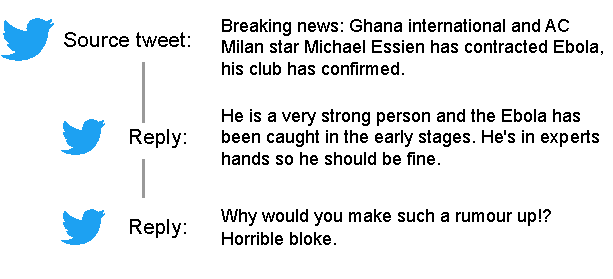
\includegraphics[scale=0.9]{obrazky-figures/pheme_essien.pdf}
    \caption{Example of fake breaking news from the PHEME dataset.}
    \label{fig:pheme_essien}
\end{figure}

In these cases, the help of content-based methods is crucial. Content-based methods rely only on the content of articles. They evaluate the linguistic and visual features from their input (e.g., style of writing, sensational headlines, etc.) and can operate using only the text of articles with no additional information needed.  The purpose of this thesis is to create a content-based classifier that relies only on text and uses it to compute the credibility of news articles and sources. The research goals can be defined as follows. (i) Understand how well can modern content-based approaches perform. (ii) Implement a method that interprets the results of the classifier to better understand what cues are exploited in the text. (iii) Use the classifier to determine the overall credibility of news publishers based on the articles they publish and compare the results with a state-of-the-art method. An interpretable classifier like this could be then used on downstream tasks, e.g., to improve available fact-checking systems by assigning a reliability score to the documents used as evidence. It could also be used to create a credibility ranking system for online sources that could even lead to creating a database of all internet publishers and their corresponding credibilities.

Chapter \ref{chap:definition} defines the problem of fake news detection and further explains the approaches and methods previously used by others in this field. Chapter \ref{datasets} presents a comprehensive review and analysis of publicly available datasets with fake news articles and discusses their suitability for this thesis. To train the classifier, only the NELA-2021 dataset is used in this thesis. The source-level labels in this dataset were expanded to all articles, meaning all articles received the label of the source that published them. This technique ensures a big dataset with lots of training data, however, as it is not guaranteed that all articles by an untrustworthy source are necessarily fake news, it may also bring some disadvantages. A similar technique of using source-level labels has been used by the authors of \cite{czech_paper}.

Chapter \ref{our-dataset} introduces the datasets created in this thesis and describes their preprocessing. Besides the NELA-GT-2021 dataset, another two datasets are used for testing purposes. The Merged dataset, created by merging three fake news datasets with article-level labels and the Fake News Interpretability (FNI) dataset, that was created by the author of this thesis and consists of 46 manually selected articles. The proposed methods for implementing the classifiers are described in chapter \ref{proposed-methods}. Chapter \ref{experiments} shows the evaluation results of the classifiers using multiple evaluation metrics.
Chapter \ref{chap:inter_anal} presents a qualitative analysis of the classifiers, including an interpretability analysis. In chapter \ref{chap:source_credibility} the implemented classifiers are applied to predict the reliability of media sources. Finally, chapter \ref{conclusion} provides a conclusion of this thesis together with suggestions for future work.




%%%%%%%%%%%%%%%%%%%%%%%%%%%%%%%%%%
% Previous work
\chapter{Fake News Detection}
\label{chap:definition}
This chapter provides a general introduction to the problem of fake news detection and the approaches used to implement it. The Cambridge Dictionary assigns fake news the following definition\footnote{\url{https://dictionary.cambridge.org/dictionary/english/fake-news}}.

\vspace{2mm}

\textbf{Definition 1:} Fake News --- False stories that appear to be news, spread on the internet or using other media, usually created to influence political views or as a joke.

\vspace{2mm}

Fake news is often used to manipulate and influence the opinions of readers during important events such as political elections. Other forms of fake news can be conspiracy theories or satire. 
In this thesis, a binary classifier model of fake news is created. The model expects the text of an article as its input and outputs the probability for two classes: reliable and unreliable. The output probabilities represent the credibility of the input article. The credibility of an article represents the extent to which the article can be perceived as trustworthy. The Cambridge Dictionary gives credibility the following definition\footnote{\url{https://dictionary.cambridge.org/dictionary/english/credibility}}.

\vspace{2mm}

\textbf{Definition 2:} Credibility --- The fact that someone can be believed or trusted.

\vspace{2mm}

Following is an overview of the methods previously used for fake news detection in this field. The methods could be classified into three categories based on the data they work with. They are content-based methods, knowledge-based methods and social context-based methods.
This thesis implements the approach of content-based methods. To base the decision, whether an article is reliable, solely on the style of its text is inherently not as reliable as using knowledge-based methods that verify the information written in the article against some database. There are, however, cases in which knowledge-based systems cannot be used, e.g., for recent news where none of the information written in the article can be verified. In these cases, a classifier based only on the stylistic features of text could be used complementary to a knowledge-based or a social context-based model.

\section{Content-based Methods}
For content-based methods, the actual content of the news is used to compute the credibility of the given article. These methods evaluate articles based on their linguistic or visual features. This means they extract lexical, semantic and syntactic characteristics capturing specific writing styles and sensational headlines that typically occur in fake news articles. 
Simple content-based methods often use the statistics of word occurrences in a corpus as the primary source of information. For these approaches, traditional methods like Term frequency-inverse document frequency (TF-IDF)\cite{tf-idf} can be used together with machine learning techniques, e.g., Decision trees, Support vector machines or Naive Bayes classifiers as in \cite{prev-work-dt} and~\cite{prev-work-bayes}.

Modelling the documents based only on word frequencies, however, limits the abilities of the classifiers. A much better approach is using word embeddings where the classifier knows not only the words that occur in a document but also has a sense of their meaning. These embeddings are usually represented as n-dimensional vectors trained to capture the relationships between words based on their co-occurrence in a document. The position of these vectors in this n-dimensional space then reflects their similarities. These embeddings can be created and trained directly from the text of documents using unsupervised methods like word2vec \cite{word2vec} and FastText \cite{fasttext}. It is also possible to obtain pre-trained word embeddings, e.g., the GloVe \cite{prev-work-glove} word representations.

These embeddings, however, do not exhibit the best performance because they employ fixed vectors for each word. This means that each word has only one vector representation that is the same in every context. A much better approach is using contextualized embeddings that enable multiple representations for a word based on the context of its surrounding words in the sentence. One example of a method that uses contextualized embeddings is the BERT \cite{bert} model.

The best results with content-based methods are generally achieved using deep neural networks. Using contextualized word embeddings and multiple layers of computation, they are able to exploit hidden features of documents and assess their credibility. Various neural network architectures are utilised for content-based methods.
Study \cite{prev-work-fndnet} proposed a deep convolutional neural network (FNDNet) for fake news detection. The authors used the GloVe pre-trained embeddings to create 100-dimensional word embeddings as the input for the network. The architecture consisted of 3 parallel convolutional layers whose results were concatenated together and run through several max pooling and dense layers. They used the Kaggle Fake News dataset, discussed in chapter \ref{datasets}, for training and evaluation and achieved an accuracy of 98.36\%. Achieving an accuracy of 98\% may look slightly suspicious. Therefore one of the objectives of this work is to create an interpretable classifier that would enable uncovering the biases that cause these exceedingly good results.

Authors of \cite{prev-work-dltechniques} implemented several fake news detection systems using 5 different classification techniques ---  Logistic regression (LR), Naïve Bayes (NB), Support vector machine (SVM), Random forest (RF) and a deep neural network (DNN) --- and compared their results. The experiments were performed on the LIAR dataset discussed later in this thesis in chapter \ref{datasets:liar}. The results showed that the DNN classifier outperformed the other traditional machine learning methods as it achieved an accuracy of 91\% followed by the NB method which achieved an accuracy of 89\%.

In both of the mentioned methods, the models were trained using pairs of text and a label that represents its credibility. A different approach was chosen by the authors of \cite{bert-exbake}. Their approach tried to detect fake news by classifying the stance of the text in the body of an article relative to its headline. The body can either agree, disagree, discuss or be unrelated to the headline resulting in 4 different class labels. To train the model they used the FNC-1\footnote{\url{https://github.com/FakeNewsChallenge/fnc-1}} dataset.
The training set consisted of a total of 2587 pairs of headline and body texts and the class label for each pair. The authors used the BERT model with its pre-trained embeddings and fine-tuned the model by classifying the data using linear and softmax layers into the four classes. Weighted cross-entropy was used as the loss function because of a big imbalance in the class labels. The classifier achieved an F1 score of 0.74.


\section{Knowledge-based Methods}
On the other hand, knowledge-based methods use external sources to check the veracity of claims extracted from the articles. This process is also known as automated fact-checking and usually consists of three stages as described in \cite{prev-work-fact-checking}: (i) claim detection to identify claims that require verification; (ii) evidence retrieval to find sources supporting or refuting the claims; (iii) claim verification to assess the veracity of the claim based on the retrieved evidence.

In other words, automated fact-checking creates evidence-grounded systems which for a given claim identify relevant sources and then use these sources to predict the veracity of the given claim.\cite{claim-dissector}.
The authors of \cite{fever} introduced a new dataset suitable for verification against textual sources called FEVER (Fact Extraction and VERification). This dataset is further described in section \ref{datasets:fever}. Other widely used datasets include FaVIQ \cite{faviq} and REALFC \cite{realfc}. Most state-of-the-art systems are based on a 3-stage approach as described in \cite{claim-dissector}: for a claim, they retrieve relevant documents, rank parts of these documents based on their relevance and predict the veracity of the given claim from the top-K ranked parts.
Another approach was introduced by the authors of \cite{claim-dissector}. They created a latent variable model called Claim-Dissector. This model combines the ranks of top-relevant, top-supporting and top-refuting provenances\footnote{Parts of the text, sentences, paragraphs, etc.} and predicts the veracity of a claim as the linear combination of its per-provenance probabilities.

\section{Social Context-based Methods}
Social context-based methods are often applied to social media as they incorporate features from user profiles to the fake news detection problem. They often use previous interactions of users and model their tendency to share information from doubtful sources. The datasets used by these methods are often collected from social media networks like Twitter or Facebook. One of these datasets is the PHEME dataset described in section \ref{datasets:pheme}. It consists of a collection of rumours and non-rumours posted during breaking news on Twitter. Besides the tweets, the dataset also contains additional information about users — their time zones, locations, number of followers, profile pictures, etc.

Social context methods usually aim to extract information by analysing the connectivity of users and articles. To do this they often use Bayesian probability graphical models as in \cite{unsupervised_graph}, or various types of matrix and tensor factorization \cite{tensor_paper}, \cite{trifn}. 

Matrix factorization is a technique commonly used also among recommender systems. In this case, the matrix composes of interactions between users (rows of the matrix) and articles (columns of the matrix). The actual values inside the matrix can be the number of interactions, minutes spent reading, a rating, etc. The interaction matrix is then decomposed as the product of two or three matrices such that it maps both users and articles to a joint latent factor space where the interactions are modelled as the inner product in that space. Examples of these models include LDA \cite{lda} and SVD \cite{svd}.
For fake news detection, a similar approach can be used. The interaction matrix is decomposed into a matrix of user and article features. New interactions can be modelled as the product of a user-feature vector and an article-feature vector resulting in a probability of this user sharing the article. 

Authors of \cite{tensor_paper} proposed a semisupervised approach for classifying fake news posts that combines tensor factorization and classification in a joint learning process. The interactions of users with posts and users with other users are modelled in a 3rd-order tensor. To decompose this tensor they employ the Canonical/Parafac (CP) factorization \cite{parafac} using a least-squares loss. The tensor is decomposed into three matrices A, B, and C, where A represents the posts-factor matrix, and B and C represent the users-factor matrices. To capture the class information of posts a classification error term is added to matrix A.

Authors of \cite{trifn} described the process of fake news dissemination on social media as a tri-relationship --- the relationship among publishers, news pieces, and users. They created an embedding model called TriFN, which models these relationships simultaneously for fake news detection.
It consists of five major components: a news contents embedding component, a user embedding component, a user-news interaction embedding component, a publisher-news relation embedding component, and a semi-supervised classification component
The news contents embedding component is a bag-of-words feature matrix. The user embedding component is constructed as a user-user adjacency matrix, that represents friendships among users. The user-news component is a matrix that states which users shared which news articles, similar to the publisher-news component that models which articles were published by which publishers. The semi-supervised classification component learns to predict unlabeled news articles. The components then employ various factorization approaches, e.g., nonnegative matrix factorization, to create feature vectors that are then used in the TriFN embedding. 

Social context-based methods are often used in combination with content-based approaches to utilize their best abilities and further improve fake news detection. Authors of \cite{hybrid} created a hybrid model based on integrating a graph neural network on the propagation of news and bi-directional encoder representations from the transformers model on news content. 

\section{Methods for Source Credibility}
This thesis studies predicting the credibility of both articles and the media sources that publish them. The credibility of sources has also been researched in previous work. In \cite{source-reputation}, the authors created an interpretable joint graphical model for fact-checking from crowds which uses claims, headlines and sources. Each claim has an assigned veracity (correctness) that can be true, false or unknown. Each headline corresponds to a source and has a stance towards the claim. The stance can be for, against or merely observing the claim. To predict the veracity of claims the authors defined a multiclass logistic regression model parameterized by R (the reputation of a source), that uses all source stances for the claim as features. In this scheme, the reputation of source R is a parameter learned by the model.

Another approach was applied by the authors of \cite{declare} who created a neural network model called DeClarE that predicts the credibility of claims by aggregating signals from external evidence articles, the language of these articles and the trustworthiness of their sources. To predict the credibility of a claim the architecture combines the article and claim embeddings to get the claim-specific attention weights. The article embeddings are run through bidirectional LSTM to create article representations. These representations are combined with the attention weights and concatenated with the claim-source embeddings and the article-source embeddings. This is then passed through several dense layers and softmax to predict the credibility of the claim. After training the model, the authors analysed the learned article-source and claim-source embeddings using PCA to project the representations. They found that fake news sources were separated from mainstream media and sources with similar opinions were located close to each other in the embedding space.

The methods of predicting the credibility of sources implemented in this thesis are compared with another method which uses the citations between sources to assess their credibility. This method is briefly explained in chapter \ref{chap:source_credibility}.



%%%%%%%%%%%%%%%%%%%%%%%%%%%%%%%%%%
% Analysis of available datasets
\chapter{Fake News Datasets}
\label{datasets}
An extensive part of this thesis was to create a review of available fake news datasets. Choosing the right dataset is crucial for training a model that generalizes as much as possible, without focusing on irrelevant biases, as explained in \cite{debias}. It was first necessary to define the requirements of our system. The chosen dataset should consist of news articles and contain the following fields: (i) the text of the article; (ii) a binary label identifying whether the article is true or fake; (iii) optionally also the name of the source that published the article. This section provides a thorough analysis of several publicly available datasets. Each dataset was evaluated for its suitability for this thesis.

Table \ref{tab:datasets_comp} shows a comparison of the studied datasets. For training the models, the NELA-GT-2021 dataset was used in this thesis. Apart from NELA, other datasets were used. The Fake news dataset, Fake or real news dataset and FakeNewsNet were merged and used for further testing of the created models. The following sections discuss the datasets in further detail.

\begin{table}[H]
    \centering
\begin{tabular}{c|c|c|c|c|}
\textbf{Dataset} & \cellcolor[HTML]{FFFFFF}\textbf{Type} & \textbf{Size} & \cellcolor[HTML]{FFFFFF}\textbf{Labels} & \textbf{Sources} \\ \hline
Fake News          & news articles & 20,800      & 2  & No  \\
Fake or Real News  & news articles & 6,335       & 2  & No  \\
NELA-GT-2021       & news articles & 1,8 million & 3* & Yes \\
FakeNewsNet        & news articles & 422         & 2  & Yes \\
Liar               & statements    & 2,836       & 6  & -   \\
FEVER              & statements    & 185,445     & 3  & -   \\
PHEME              & tweets        & 6,425       & 2  & -   
\end{tabular}    
    \caption{Comparison of the examined datasets. *The labels in the NELA dataset are on a source level (label per source, not per each article).}
    \label{tab:datasets_comp}
\end{table}


\section{Fake News Dataset}
\label{fake_news_dataset}
The first reviewed dataset is called the Fake news dataset. It was published in 2018 and is available on the Kaggle website\footnote{\url{https://www.kaggle.com/competitions/fake-news/data}}. There is no specific information available on how this dataset was collected. The author only stated that it was created by merging several fake news datasets available on Kaggle and that he would not vouch for its quality in general as it may contain lots of artefacts that limit its usefulness in training a more generalizable model. Despite this knowledge. the dataset was used in some publications, including \cite{prev-work-fndnet}. Table \ref{tab:fake_news_table} shows the fields in the training dataset.

% \begin{itemize}
%     \item id = unique id for a news article
%     \item title = the title of the article
%     \item author = author of the article
%     \item text = text of the article; could be incomplete
%     \item label = binary label that marks the article as potentially unreliable (1-unreliable, 0-reliable)
% \end{itemize}

\begin{table}[H]
    \centering
\begin{tabular}{c|c|l}
\rowcolor[HTML]{FFFFFF} 
\textbf{Column} & \textbf{Type}                  & \textbf{Description}                \\ \hline
title           & text                           & Headline of the article             \\
author          & text                           & Author of the article               \\
text            & text                           & The text in the body of the article \\
label & integer & \begin{tabular}[c]{@{}l@{}}Binary label that marks the article as potentially unreliable \\ (1---unreliable, 0---reliable)\end{tabular}
\end{tabular}
    \caption{Fields inside the Fake News Dataset.}
    \label{tab:fake_news_table}
\end{table}

The test dataset contains the same fields except for the labels, as the results were meant to be submitted to the authors for evaluation. One drawback of this dataset is that the articles contain no sources. The only available information is the name of the author, which is not a useful feature with respect to the aims of this thesis.

The training dataset contains 20,800 articles and the test dataset 5,200 articles. The distribution of reliable and unreliable articles is well-balanced. The articles contain on average 773 words. The topic of the articles is not specified. After analysing the most used words it can be assumed that most articles revolve around politics, most probably in the U.S. as the most common words were Donald Trump, Hillary Clinton, America and the United States.


\section{Fake or Real News Dataset}
\label{fake_or_real_news}
Fake or real news is a small dataset presented in \cite{fake_or_real_dataset} as part of their survey on fake news prediction. It is available on Kaggle.com\footnote{\url{https://www.kaggle.com/datasets/rchitic17/real-or-fake}}. The dataset consists of 6,335 news articles. Each article is assigned a binary label identifying it as either real or fake. The distribution of labels is well-balanced with approximately half of the articles being real and the other half fake. The dataset contains the following fields.


\begin{table}[H]
\centering
    \begin{tabular}{c|c|c}
    \textbf{Column} & \cellcolor[HTML]{FFFFFF}\textbf{Type} & \cellcolor[HTML]{FFFFFF}\textbf{Description} \\ \hline
    title & text & Headline of the article             \\
    text  & text & The text in the body of the article \\
    label & text & Binary label (REAL/FAKE)           
    \end{tabular}
    \label{tab:fake_or_real_fields}
    \caption{Fields for each article in the Fake or real news dataset.}
\end{table}


In some cases, the text contains the name of the author or media source that published the article. However, for most articles, this information is unknown. The topics of the articles are also not known.


\section{NELA-GT-2021}
\label{nela}
This section discusses the NELA-GT-2021 dataset\footnote{\url{https://dataverse.harvard.edu/dataset.xhtml?persistentId=doi:10.7910/DVN/RBKVBM}}. The 2021 version of the NELA-GT dataset is the fourth publication of this dataset and is further described by the authors in~\cite{nela-paper}. 
The dataset was created by scraping the content of web articles from news sources on the internet published in 2021. It consists of approximately 1.8 million articles from 348 different sources. The scraped articles contain the following fields.

\begin{table}[H]
    \centering
\begin{tabular}{c|c|l}
\rowcolor[HTML]{FFFFFF} 
\textbf{Column} & \textbf{Type}               & \textbf{Description}                              \\ \hline
id              & text (primary key)          & Identifier of the article                         \\
date            & text                        & Publication date string in yyyy-mm-dd format      \\
source          & text                        & Name of the source that published the article     \\
title           & text                        & Headline of the article                           \\
content         & text                        & The text in the body of the article               \\
author          & text                        & Author of the article (may be empty)              \\
published       & text                        & Publication date string as provided by the source \\
published\_utc  & integer                     & Publication time as unix time stamp               \\
collection\_utc & integer                     & Collection time as unix time stamp                \\
url             & text                        & URL of the article                               
\end{tabular}
    \caption{Structure of data collected for an article in the NELA-GT-2021 dataset.}
    \label{tab:nela_fields}
\end{table}

An important part of the dataset, besides the actual content of the scrapped articles, is a categorization of the collected news sources. In a separate file, called labels.csv, there is a label for each source defining its reliability. The label can have one of the following values.

\begin{itemize}
    \item 0 --- marks the given source as reliable
    \item 1 --- marks the given source as unreliable
    \item 2 --- marks the given source as mixed
\end{itemize}

To create these source-level labels, the authors of the dataset used a website specialized in rating news sources on the internet called Media Bias / Fact Check (MBFC)\footnote{\url{https://mediabiasfactcheck.com/}}. This website contains an extensive database of more than 5400 media sources and journalists, categorized by two main criteria: bias and factuality. 
The \emph{bias of a news source defines a prejudice or an inclination in favour of or against one thing, person or group}. The MBFC website recognizes the following types of bias:

\begin{itemize}
    \item Least Biased --- Most credible media sources that have minimal bias, factual reporting and are usually well sourced.
    
    \item Left Bias ---  Moderately to strongly biased toward liberal causes through story selection and/or political affiliation. These sources may be misleading and untrustworthy.
    
    \item Left-Center Bias --- Slight to moderate liberal bias, usually trustworthy sources.

    \item Right Bias --- Moderately to strongly biased toward conservative causes through story selection and/or political affiliation. These sources may be misleading and untrustworthy.

    \item Right-Center Bias --- Slight to moderate conservative bias, generally trustworthy.

    \item Conspiracy-Pseudoscience --- These sources publish unverifiable information that is usually not supported by evidence, may be untrustworthy.

    \item Questionable Sources --- Extreme bias, promotion of propaganda and conspiracies, no sourcing of credible information and fake news. These sources are very untrustworthy.

    \item Pro-Science --- These sources publish evidence-based information through the use of credible scientific sourcing. Unbiased and trustworthy.

    \item Satire --- These sources use humour, irony, exaggeration, or ridicule to expose and criticize people or other topics. They usually claim to be satirical and do not try to deceive.
\end{itemize}

The bias of media sources may help to identify not only the inclination towards specific topics but also the credibility of published articles. The MBFC website recognises two main biases of untrustworthy sources: Conspiracy-Pseudoscience and Questionable Sources, with the latter being marked as likely very untrustworthy. On the other hand, sources marked as Pro-science or Least Biased can be generally considered credible. 
Another measure that the MBFC website uses to classify media sources is the factuality score. \emph{Factuality represents how much the reporting of a source resolves around actual well-sourced facts that can be proven}. It may hold one of the following six values:

\begin{multicols}{2}
\begin{itemize}
    \item Very Low
    \item Low
    \item Mixed
    \item Mostly Factual
    \item High
    \item Very High
\end{itemize}
\end{multicols}

A source with a very low or low factuality could be considered untrustworthy, whereas sources with very high or high factualities are likely to publish credible information. The final labels of a given media source in the NELA-GT-2021 dataset are constructed as follows: \cite{nela-paper}

\begin{itemize}
    \item 0 (reliable) --- sources with high or very high factuality
    \item 1 (unreliable) --- sources with Conspiracy-Pseudoscience bias or very low / low factuality
    \item 2 (mixed) --- sources with mixed factuality
\end{itemize}

The distribution of source labels in the dataset can be seen in figure \ref{fig:labels_all_dist}. As the figure shows, the distribution of media sources among labels is not very even. The number of unreliable sources is more than double the number of reliable and more than four times the number of sources marked with the mixed label. This proportion changes when looking at the total number of articles for each label. \emph{There are more unreliable sources but more reliable articles in the dataset}. In total, the dataset contains 603,894 articles from reliable sources, 490,345 articles from unreliable sources and 416,673 articles from mixed sources as shown in figure \ref{fig:articles_per_label}.

\begin{figure}[H]
\centering
\begin{subfigure}{.5\textwidth}
  \centering
  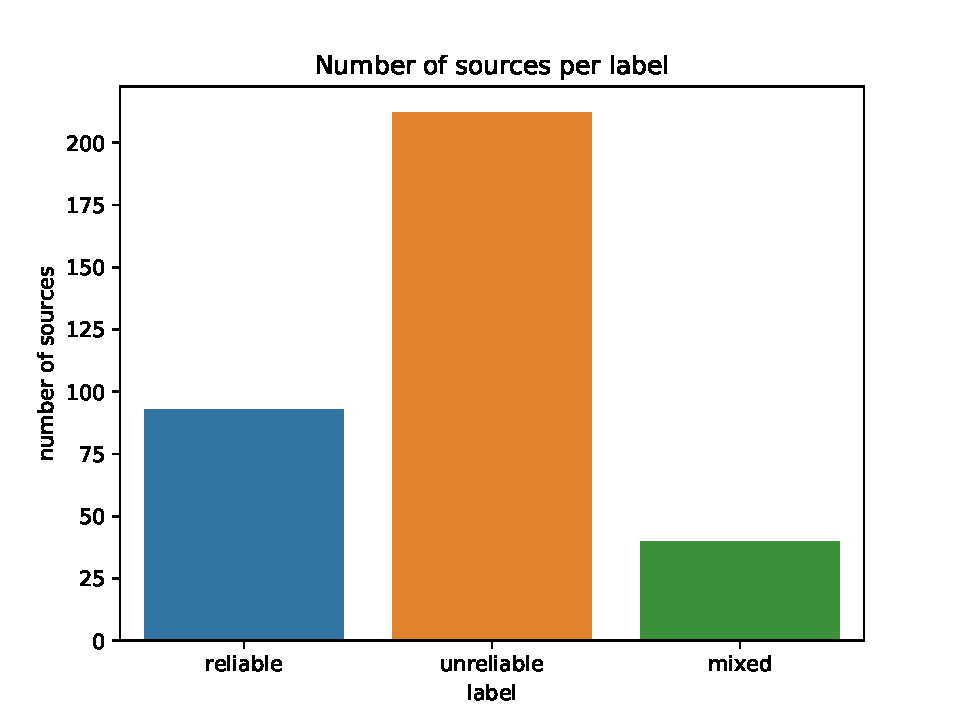
\includegraphics[width=\linewidth]{obrazky-figures/labels_all_dist.pdf}
  \caption{The number of sources per label.}
  \label{fig:labels_all_dist}
\end{subfigure}%
\begin{subfigure}{.5\textwidth}
  \centering
  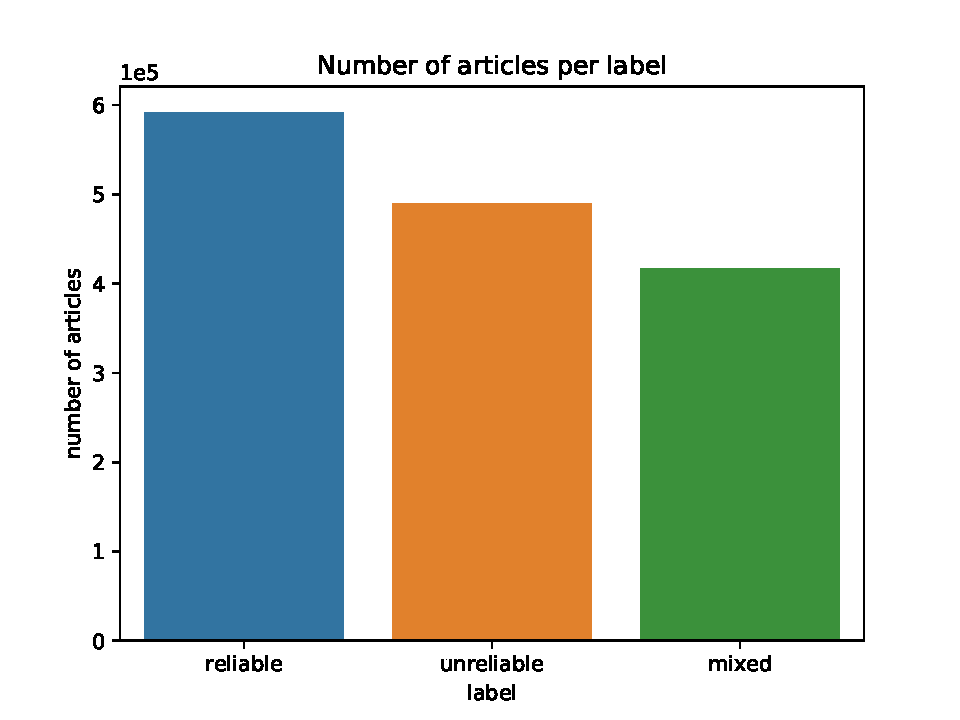
\includegraphics[width=\linewidth]{obrazky-figures/articles_per_label.pdf}
  \caption{The number of articles per label.}
  \label{fig:articles_per_label}
\end{subfigure}
\caption{Distribution of labels in the NELA-GT-2021 dataset.}
\label{fig:test}
\end{figure}

Due to the imbalance in the distribution of labels, it is obvious that the most frequent types of bias are the ones that imply untrustworthy sources. Indeed the most common bias in the dataset is Conspiracy-Pseudoscience, followed by the Questionable Source and Left-Center bias. The number of sources per bias is shown in figure \ref{fig:bias_dist}.
It is also interesting to see what are the most common biases in each label group. As already mentioned earlier, sources labelled as unreliable are those with Conspiracy-Pseudoscience bias or low/very low factuality. It is therefore straightforward that the most common biases among unreliable sources are Conspirtacy-Pseudoscience (159 sources), Questionable-Source (52 sources) and one source with Right bias. 
Reliable sources, on the other hand, contain sources from 6 different biases: Left-Center (40 sources), Left (18 sources), Center (13 sources), Right-Center (12 sources), Pro-Science (6 sources), Right (4 sources). 
Sources with the Mixed label are also spread between several biases: Right (17 sources), Left-Center (11 sources), Left (11 sources) and Right-Center (1 source). The number of sources per bias in each label can be also seen in figure \ref{fig:bias_by_src}

\begin{figure}[H]
    \centering
    \begin{subfigure}{.5\textwidth}
      \centering
      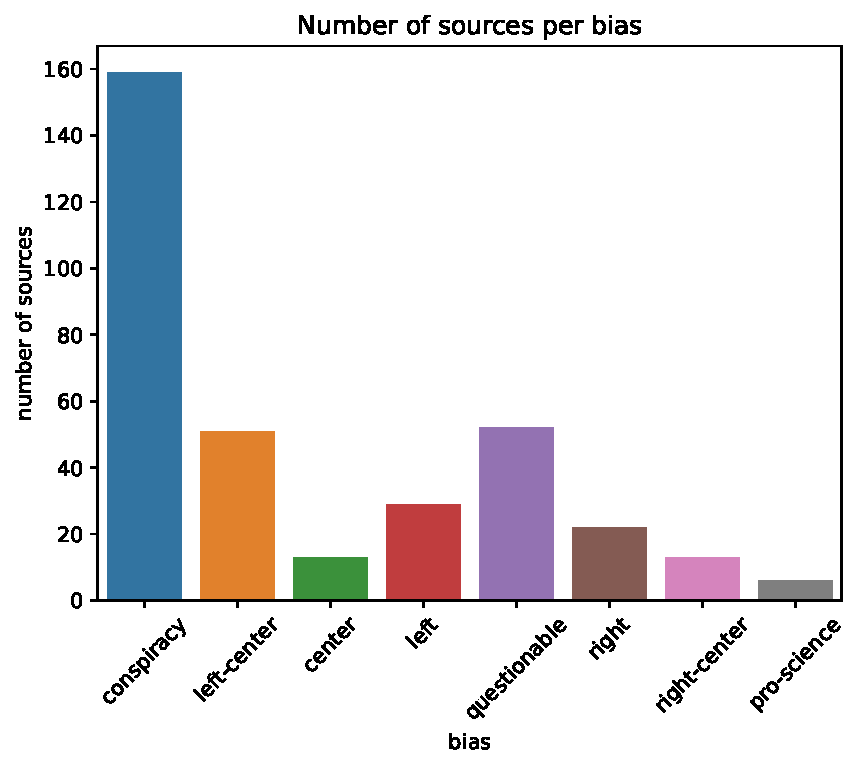
\includegraphics[width=\linewidth]{obrazky-figures/bias_dist.pdf}
      \caption{Number of sources per bias.}
      \label{fig:bias_dist}
    \end{subfigure}%
    \begin{subfigure}{.5\textwidth}
      \centering
      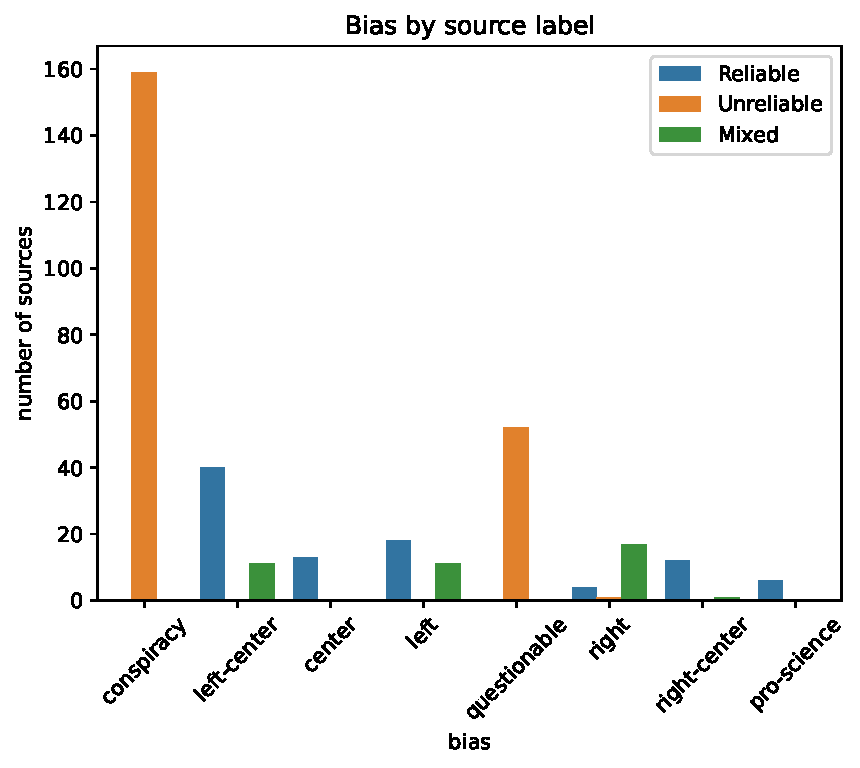
\includegraphics[width=\linewidth]{obrazky-figures/bias_by_src.pdf}
      \caption{Number of sources per bias for each label.}
      \label{fig:bias_by_src}
    \end{subfigure}
    \caption{Analysis of the sources and their bias in the NELA-GT-2021 dataset.}
    \label{fig:test2}
\end{figure}

Similarly, we can have a look at the number of sources per factuality score. This can be seen in figure \ref{fig:factuality_dist}. Figure \ref{fig:factuality_by_src} then shows the number of sources per factuality for each label. It is evident that sources labelled as unreliable generally possess lower factuality scores. Interestingly, there is one source with mixed factuality marked as reliable (Daily Telegraph - UK). 

\begin{figure}[H]
    \centering
    \begin{subfigure}{.5\textwidth}
      \centering
      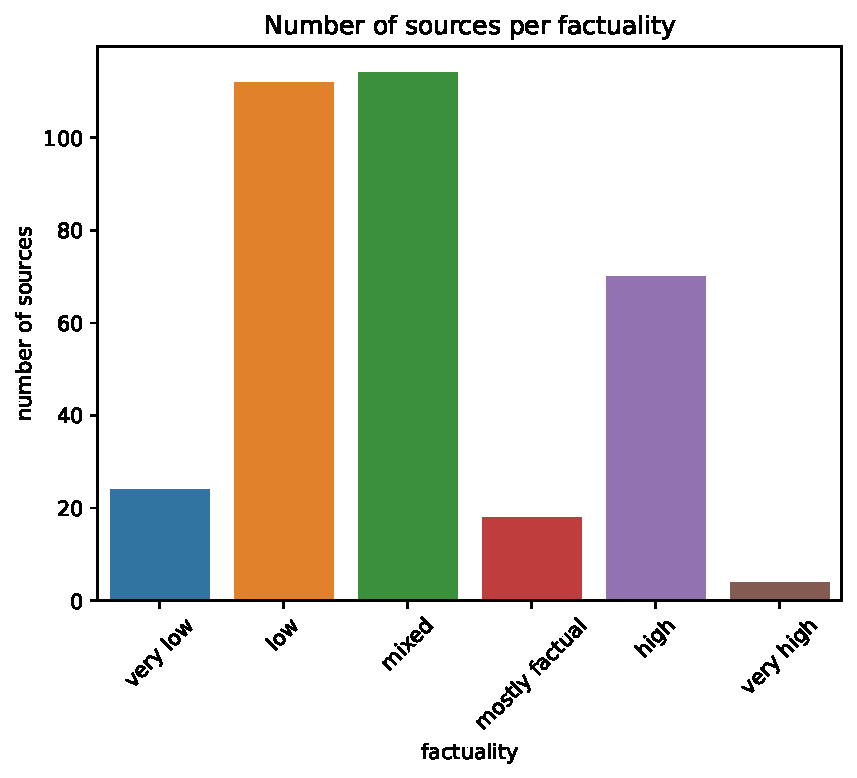
\includegraphics[width=\linewidth]{obrazky-figures/factuality_dist.pdf}
      \caption{Number of sources per factuality score.}
      \label{fig:factuality_dist}
    \end{subfigure}%
    \begin{subfigure}{.5\textwidth}
      \centering
      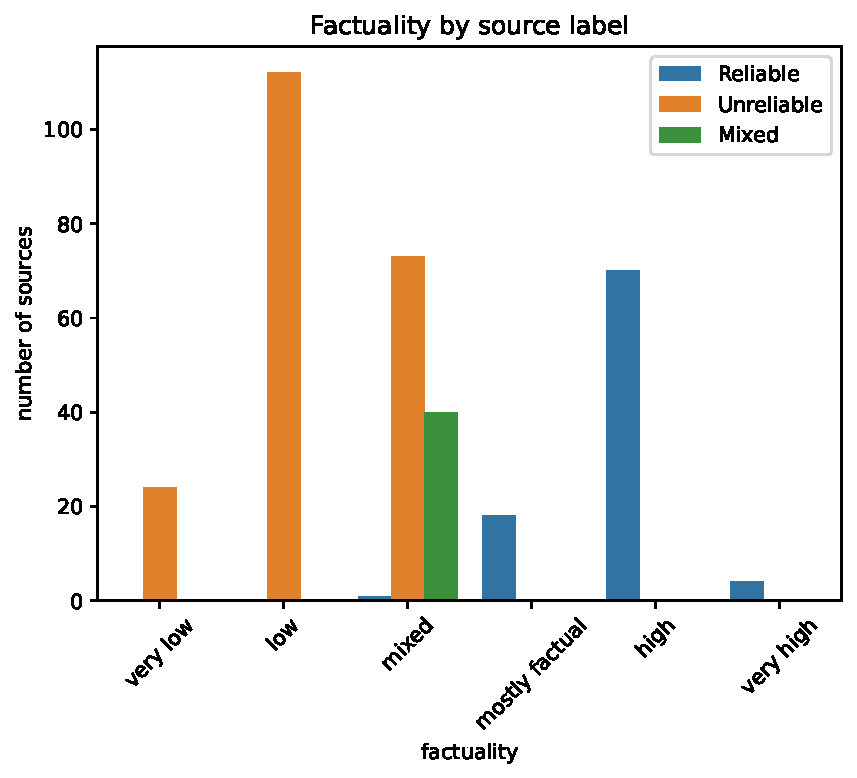
\includegraphics[width=\linewidth]{obrazky-figures/factuality_by_src.pdf}
      \caption{Number of sources per factuality for each label.}
      \label{fig:factuality_by_src}
    \end{subfigure}
    \caption{Analysis of the sources and their factuality score in the NELA-GT-2021 dataset.}
    \label{fig:test3}
\end{figure}

The actual content of articles in the NELA dataset had to be slightly modified as some of the texts in the dataset are copyrighted. For articles with more than 200 tokens, 7 consecutive tokens are replaced with an at symbol ‘@’ every 100 tokens. For articles with fewer than 200 tokens, only 5 tokens are replaced with ‘@’ every 20 tokens. This transformation polishes the articles to make them useless for anyone who would want to use the dataset to consume news while still keeping most of the content useful for analysis. Features like the relative frequency of words are not affected by this transformation as it occurs with no regard to context. Following is an example of the polished text in the dataset:

\begin{center}
    \texttt{The proposals are primarily in response to President Joe Biden ’ s @ @ @ @ @ @ @ least 100 employees to get vaccinated or tested regularly. Randy Zook , president of the state Chamber of Commerce , warned lawmakers that the proposal could force employers between choosing whether to violate state law or federal regulations.}
\end{center}

The NELA-GT-2021 dataset was found suitable for this thesis. It is a large dataset with source-level labels and besides the content of articles, it contains additional information about where and when they were published. Polishing the text with special symbols should have no effect on the analysis. More details about how this dataset is used in this thesis can be found in chapter \ref{our-dataset}.


\section{FakeNewsNet}
\label{fake_news_net}
FakeNewsNet is a dataset available at Kaggle.com\footnote{\url{https://www.kaggle.com/code/sohamohajeri/buzzfeed-news-analysis-and-classification/data}}. It consists of 422 news articles collected by Buzzfeed\footnote{\url{https://www.buzzfeed.com/}} and Politifact\footnote{\url{https://www.politifact.com/}}. Each article is assigned a binary label indicating whether the article is real or fake. Besides labels, this dataset contains additional information, some of which is displayed in table \ref{tab:fakenewsnet}.


\begin{table}[H]
    \centering
    \begin{tabular}{c|c|l}
    \textbf{Column} & \cellcolor[HTML]{FFFFFF}\textbf{Type} & \cellcolor[HTML]{FFFFFF}\textbf{Description} \\ \hline
    title        & text & Headline of the article             \\
    text         & text & The text in the body of the article \\
    url          & text & Url of the article                  \\
    authors      & text & Names of authors of the article     \\
    source       & text & Source that published the article   \\
    publish date & text & Publication date of the article     \\
    movies       & text & Urls to all videos in the article   \\
    images       & text & Urls of all images in the article  
    \end{tabular}
    \caption{Fields in the FakeNewsNet dataset.}
    \label{tab:fakenewsnet}
\end{table}

The distribution of labels is very well-balanced with half of the articles being fake and the other half real. This dataset is a great candidate for the purposes of this thesis. It consists of news articles and contains both labels and sources. However, due to its size of only 422 articles, it may not be enough to train a robust classifier and it is therefore only used for testing.


\section{Liar Dataset}
\label{datasets:liar}
Introduced in \cite{liar}, the Liar dataset consists of 12,836 statements collected in various contexts from politifact.com. Each statement was manually assigned a label evaluating it for its truthfulness. The dataset considers six fine-grained labels, in order from less to most trustworthy: pants-fire, false, barely-true, half-true, mostly-true, and true. The average length of a statement in the dataset is 18 words.
The statements in the dataset are categorized into 4,535 different subjects. The most common ones are health care, taxes, education, elections and immigration. Each statement also specifies the speaker, meaning the person responsible for the statement. The most common speakers in the dataset are Barack Obama, Donald Trump, Hillary Clinton and Mitt Romney. Table \ref{tab:liar_columns} shows all fields in the Liar dataset.
\begin{table}[h]
    \centering
    \begin{tabular}{c|c|l}
    \textbf{Column} & \cellcolor[HTML]{FFFFFF}\textbf{Type} & \cellcolor[HTML]{FFFFFF}\textbf{Description}  \\ \hline
    label       & text    & Label of the statement                  \\
    statement   & text    & Content of the evaluated statement      \\
    subject     & text    & The topic/subject of the statement      \\
    speaker     & text    & Name of the speaker                     \\
    speaker job & text    & Job title of the speaker                \\
    state       & text    & State which the speaker is representing \\
    party       & text    & Party affiliation of the speaker        \\
    barely-true & integer & Barely-true counts                      \\
    false       & integer & False counts                            \\
    half-true   & integer & Half-true counts                        \\
    mostly-true & integer & Mostly-true counts                      \\
    pants-fire  & integer & Pants on fire counts                    \\
    venue           & text                                  & The venue/location of the speech or statement
    \end{tabular}
    \caption{Structure of data in the Liar dataset.}
    \label{tab:liar_columns}
\end{table}
The barely-true, false, half-true, mostly-true, and pants-fire fields in the dataset, represent the total number of statements by the speaker that were assigned the given label. Figure \ref{fig:liar_labels} shows the number of statements for each label. The distribution of labels is well-balanced except for the pants-fire label. 
\begin{figure}[h]
    \centering
    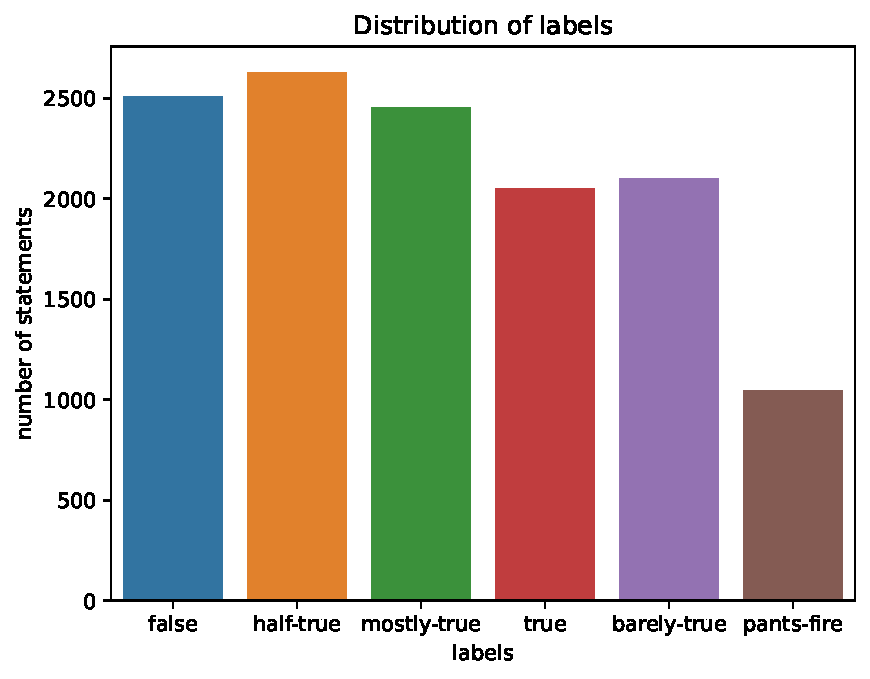
\includegraphics[scale=0.6]{obrazky-figures/liar_labels.pdf}
    \caption{Number of statements by label in the Liar dataset.}
    \label{fig:liar_labels}
\end{figure}

The Liar dataset is one of the most used datasets for fake news detection. Its manually assigned labels guarantee a big level of authenticity. However, as the dataset only contains short statements, it is not suitable for training a classifier working with entire news articles. Therefore, it was not found suitable for the purpose of this thesis.


\section{FEVER}
\label{datasets:fever}
FEVER, which stands for Fact Extraction and Verification, is a dataset for verification against textual sources introduced in \cite{fever}. The dataset consists of 185,445 claims generated by altering sentences extracted from Wikipedia. For each claim, there is evidence that can be used to verify it. The claims are labelled as Supports, Refutes or Not enough info indicating whether the evidence supports or refutes the claim. On average, a claim contains only 8 words. Some examples of claims from the FEVER dataset are:

\begin{center}
    \texttt{Roman Atwood is a content creator.} \\
    \texttt{Charles Woodruff Yost died.} \\
    \texttt{Portugal leads the European Union.} \\
    \texttt{Muhammad Ali was a model of racial pride for resistance to white domination.}
\end{center}

\begin{table}[H]
    \centering
    \begin{tabular}{c|c|l}
    \textbf{Column} & \cellcolor[HTML]{FFFFFF}\textbf{Type} & \cellcolor[HTML]{FFFFFF}\textbf{Description} \\ \hline
    verifiable & text & Specifies whether given claim is verifiable or unverifiable  \\
    label      & text & Specifies whether the evidence refutes or supports the claim \\
    claim      & text & The evaluated claim                                          \\
    evidence   & text & Reference to the evidence refuting or supporting the claim  
    \end{tabular}
    \caption{Structure of data in the FEVER dataset.}
    \label{tab:fever_columns}
\end{table}

Table \ref{tab:fever_columns} shows the contents of the FEVER dataset. Figure \ref{fig:fever_labels} shows the distribution of labels in the dataset. It may be seen that the majority of claims are supported by the evidence as the number of claims in this class is more than double the number of claims that are refuted. 

\begin{figure}[H]
    \centering
    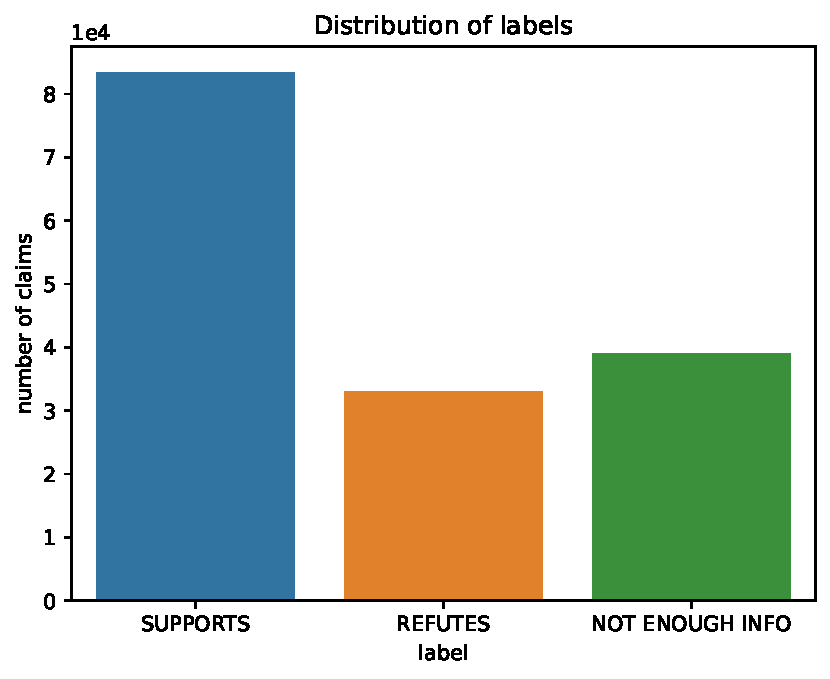
\includegraphics[scale=0.6]{obrazky-figures/fever_labels.pdf}
    \caption{Number of claims by label in the FEVER dataset.}
    \label{fig:fever_labels}
\end{figure}

The main use of the FEVER dataset is for fact-checking and extraction tasks. It could, however, also be used for fake news detection tasks as the labels that indicate whether the evidence supports or refutes the claim, could also be interpreted as whether the claim is true or fake. This interpretation would enable the training of a classifier. However, given the short nature of given claims, it is not suitable for classifying long texts of news articles.



\section{PHEME}
\label{datasets:pheme}
PHEME was introduced in \cite{pheme}. It is a dataset containing a collection of rumours and non-rumours posted during breaking news related to 9 different events on Twitter. Besides the tweets, the dataset also contains information about the authors of the tweets, their locations, number of followers, links to their profiles etc. The dataset also contains all the reactions to the posted rumours/non-rumours tweets including comments and likes. 
In total, there are 4,023 non-rumour and 2,402 rumour tweets. This dataset is ideal for use in social context-based methods where the classifier evaluates the interactions of users. It is, therefore, not suitable for this thesis.



%%%%%%%%%%%%%%%%%%%%%%%%%%%%%%%%%%
% Analysis of the test dataset
\chapter{Creating Datasets For This Thesis}
\label{our-dataset}
The previous chapter analyzed available fake news datasets. This chapter presents the final datasets that are used for training and testing the classifiers in this thesis. In total, three different datasets are used. The dataset used for training is a preprocessed form of the NELA-GT-2021 dataset. The other two datasets are used only for testing. These datasets are the Merged dataset --- created by merging three different fake news datasets --- and the Fake News Interpretability dataset ---  created especially for this thesis by manually collecting several fake and real articles.




\section{NELA Dataset}
\label{nela-my}
The dataset used for training the classifiers in this thesis was created by modifying the NELA-GT-2021 dataset. This section describes the preprocessing of this dataset as displayed in figure \ref{fig:nela_prepproc}. The first step was expanding the source-level labels to all articles. This means that all articles were assigned the label of their source. After expanding the labels, all articles labelled as mixed were removed. Only the articles published by reliable and unreliable sources were kept in the dataset. The reason for removing mixed labels is that the articles published by mixed sources may contain both reliable and unreliable articles, making it harder for the classifier to correctly learn to detect fake news. 
% The experiments performed on a classifier trained with mixed labels showed a significant degradation in the performance and it is further discussed in chapter \ref{experiments}. 

The next preprocessing step was keyword filtering. After initial manual analysis, it was found that the text often contains simple cues, e.g., source name, author name, etc., which could be leveraged by the model without analyzing the semantics of the language. To investigate the exploitation of the easy cues by the models, an analysis using the baseline model was performed. The baseline model, described in chapter \ref{baseline}, uses a Multinomial Naive Bayes (MNB) classifier and TF-IDF.
% As a consequence of extending the labels of sources to all their articles, there is a possibility that the created classifiers would actually learn to classify sources instead of labels. The classifier could, for example, learn that all articles published by CBS can be considered reliable and would therefore learn to identify keywords, e.g.,, the name of the source. 

\begin{figure}[H]
    \centering
    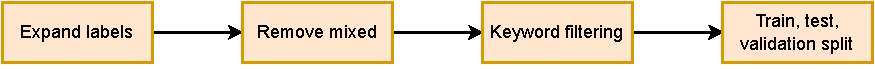
\includegraphics[scale=1]{obrazky-figures/nela_preproc.pdf}
    \caption{Preprocessing steps of the NELA dataset.}
    \label{fig:nela_prepproc}
\end{figure}

In the training process, the MNB classifier learns the probabilities of all words for each class. This means each word in the dataset is assigned a probability for classes \texttt{reliable} and \texttt{unreliable}. It is then possible to look at the words with the highest probabilities for each class and hence display the words that contribute the most to the decision of the classifier. The importance of word $x$ is computed as follows.

\begin{equation}
    \operatorname{Imp}(x) = \displaystyle{\frac{P (x | reliable)} {P (x | unreliable)}}
    \label{eq:imp}
\end{equation}
where $P (x | reliable)$ is the probability of $x$ for class \texttt{reliable} and $P (x | unreliable)$ is the probability of $x$ for class \texttt{unreliable}. Words with high values are more important to the \texttt{reliable} class and vice versa. The filtering was performed by comparing each word from the articles with a defined set of keywords. If a word matches one of the defined keywords it is removed from the text. The filtering was performed in two iterations with each iteration having its own set of keywords. The following keywords were used in the iterations.

\begin{itemize}
    \item Iteration 1 --- (395 keywords) filtering names of sources in various forms as they appear in the dataset (e.g., \texttt{cbs}, \texttt{cbsn}, \texttt{upi}, \texttt{ipolitics}, \texttt{foxnews}, \texttt{tass}, etc.).
    \item Iteration 2 --- (19 keywords) filtering source-specific terms discovered during the analysis of the most important words for each class. This includes football-related terms --- as the sources writing about football are considered reliable, the classifier learned to interpret football-related terms as a sign of reliability (especially names of players, coaches and football clubs). Other source-specific keywords include, e.g., \texttt{garda}, \texttt{gardaí} (names of the police department in Ireland used by a reliable source The Irish Times), \texttt{quijano} (name of a cbs news reporter Elaine Quijano), \texttt{paypal}, and currency abbreviations (heavily used by an unreliable source --- Infinite Unknown --- at the end of their articles where they ask readers for donations).
\end{itemize}

Table \ref{tab:kw_filtering} shows the most important words for each class in the original dataset and after keyword filtering. It can be seen that in the original dataset, there are a lot of source names among the most important words (e.g., \texttt{cbsn}, \texttt{upi}, \texttt{ipolitics}, \texttt{nrplus}, \texttt{sitsshow}, \texttt{lifesitenews}). After removing them in the first iteration, the 20 most important words, discovered with the method in equation \ref{eq:imp}, were manually analysed. Multiple source-specific terms were identified, e.g., \texttt{gardaí}, \texttt{arteta} --- the coach of Arsenal football club, currency abbreviations, etc. Therefore the second iteration was applied to remove these terms.


\begin{table}[H]
    \centering
\begin{tabular}{c|c|c|c|c|c}
\multicolumn{2}{c|}{\textbf{Original}}                        & \multicolumn{2}{c|}{\textbf{Iteration 1}}   & \multicolumn{2}{c}{\textbf{Iteration 2}}   \\ \hline
\multicolumn{1}{c|}{\textbf{reliable}} & \textbf{unreliable} & \textbf{reliable} & \textbf{unreliable} & \textbf{reliable} & \textbf{unreliable} \\ \hline
\multicolumn{1}{c|}{redistributed}     & gbp                 & redistributed     & paypal              & redistributed     & discernment         \\
\multicolumn{1}{c|}{cbsn}      & aud          & rewritten   & gbp         & rewritten     & kerth    \\
\multicolumn{1}{c|}{rewritten} & paypal       & gardaí      & aud         & lanarkshire   & donate   \\
\multicolumn{1}{c|}{upi}       & chf          & lanarkshire & chf         & notifications & longform \\
\multicolumn{1}{c|}{ipolitics} & eur          & moyes       & eur         & osborn        & flote    \\
\multicolumn{1}{c|}{moyes}     & sitsshow     & quijano     & discernment & lapook        & epoch    \\
\multicolumn{1}{c|}{nrplus}    & lifesitenews & arteta      & usd         & alerts        & peta    
\end{tabular}
    \caption{The most important words in the original dataset, after the first iteration of filtering and after the second iteration of filtering.}
    \label{tab:kw_filtering}
\end{table}

Figure \ref{fig:prc_keywords} shows the percentage of articles that contained at least one of the filtered keywords. 
It can be seen that over 60\% of unreliable articles and over 30\% of reliable articles in the dataset contained a source name in their text. The keywords from the second iteration were not as common as they only appeared in approximately 4\% of reliable and 10\% of unreliable articles.
Figure \ref{fig:prc_sources} shows the ratio of reliable, unreliable and mixed sources mentioned in the articles of the NELA dataset. Nearly 70\% of the sources mentioned in reliable articles are also reliable. Unreliable articles mention reliable sources more often than unreliable sources and around 54\% of the mentions are related to mixed sources. 

\begin{figure}[H]
    \centering
    \begin{subfigure}{.5\textwidth}
      \centering
      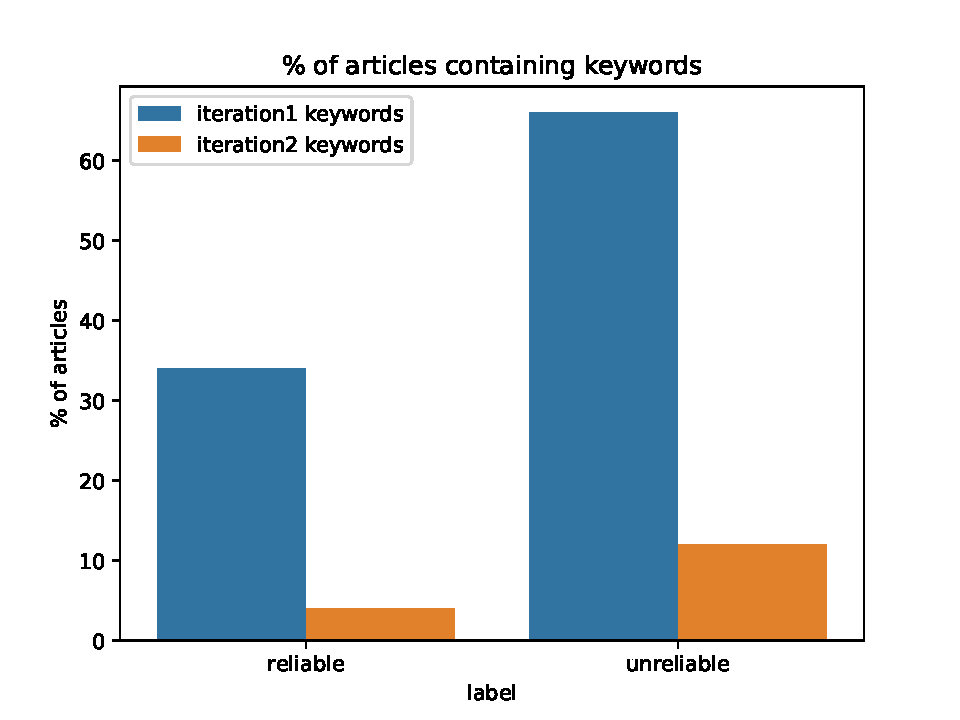
\includegraphics[width=\linewidth]{obrazky-figures/percentage_keywords.pdf}
      \caption{}
      \label{fig:prc_keywords}
    \end{subfigure}%
    \begin{subfigure}{.5\textwidth}
      \centering
      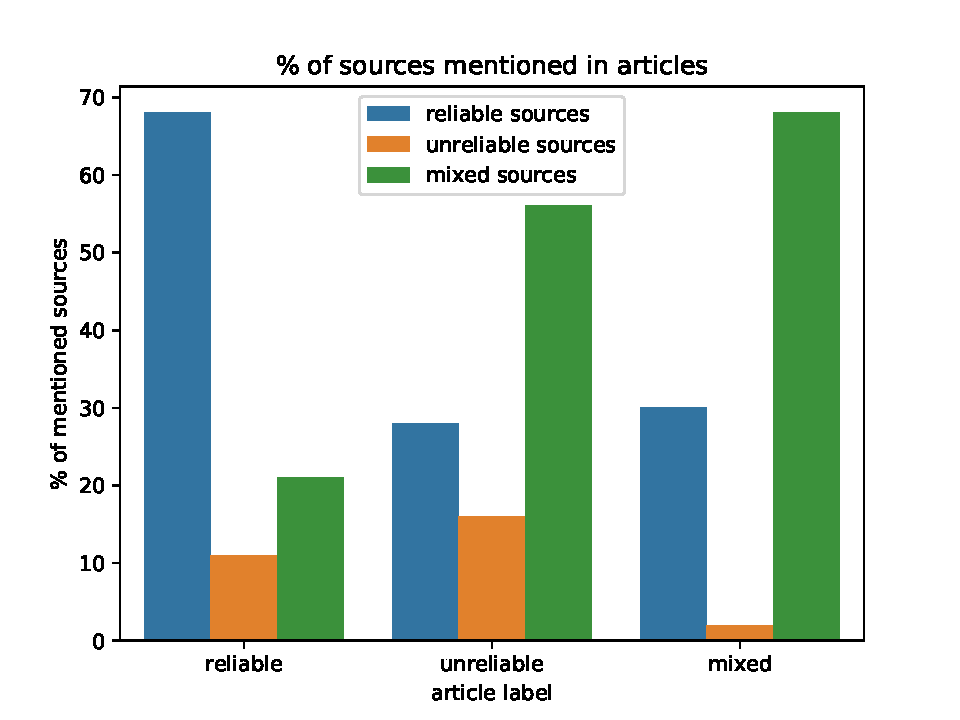
\includegraphics[width=\linewidth]{obrazky-figures/percentage_sources.pdf}
      \caption{}
      \label{fig:prc_sources}
    \end{subfigure}
    \caption{Figure (a) shows the percentage of articles that contained at least one of the filtered keywords. Figure (b) contains the percentage of sources mentioned in reliable unreliable and mixed articles.}
    \label{fig:test3}
\end{figure}

The last step of the preprocessing was creating the train, test and validation splits. The final datasets are presented in table \ref{tab:nela_split}.

\begin{table}[H]
    \centering
\begin{tabular}{|r|r|r|r|}
\hline
\textbf{Dataset} & \textbf{Reliable articles} & \textbf{Unreliable articles} & \textbf{Total} \\ \hline
train & 312,069 & 304,729 & 616,798 \\ \hline
test & 98,337 & 98,103 & 196,440 \\ \hline
validation & 78,851 & 78,346 & 157,197 \\ \hline
\end{tabular}
    \caption{Number of articles in the train, validation and test splits of the NELA dataset.}
    \label{tab:nela_split}
\end{table}


\section{Merged Dataset}
\label{sec:merged}
The NELA dataset, used for training the classifiers, uses source-level labels expanded to all articles. The Merged dataset is used to additionally test the abilities of the classifiers on a dataset whose labels were not extracted from sources. \emph{The Merged dataset was created by merging three fake news datasets with binary labels}: the Fake news dataset described in section \ref{fake_news_dataset}, the Fake or real news dataset described in section \ref{fake_or_real_news} and FakeNewsNet described in section \ref{fake_news_net}. The resulting dataset consists of 27,518 articles (13,769 reliable and 13,749 unreliable). It is intended to be used only for further evaluation of the created classifiers.



\section{Fake News Interpretability Dataset}
\label{test-dataset}
This section introduces the Fake News Interpretability (FNI) dataset created as part of this thesis. It was created for qualitative analysis and evaluation of the implemented classifiers. The FNI dataset consists of 46 manually picked articles (23 reliable, 23 unreliable). For each article, the dataset contains a label, indicating whether it is reliable or unreliable, the URL of the article, the source that published the article, bias and the factuality score of the source (if known) obtained from the MBFC website and the date of publication. The factuality score ranges from 0 (least factual reporting) to 5 (most factual reporting). Table \ref{tab:test_dataset} shows all the fields stored for each article in the dataset.

\begin{table}[H]
    \centering
    \begin{tabular}{c|c|l}
    \textbf{Column} & \cellcolor[HTML]{FFFFFF}\textbf{Type} & \cellcolor[HTML]{FFFFFF}\textbf{Description} \\ \hline
    title      & text & Headline of the article             \\
    text       & text & The text in the body of the article \\
    url        & text & Url of the article                  \\
    label      & text & Binary label (True/Fake)            \\
    source     & text & Source that published the article   \\
    topic      & text & Topic of the article                \\
    mbfc bias  & text & Bias of the source from MBFC        \\
    factuality & text & Factuality of the source from MBFC  \\
    date       & text & Date when the article was published
    \end{tabular}
    \caption{Fields in the FNI dataset.}
    \label{tab:test_dataset}
\end{table}

The fake articles were obtained from three main sources:
\begin{itemize}
    \item The top 50 fake news hits of 2016 published by Buzzfeed News in \cite{buzzfeed:fake}.
    \item The MBFC website --- cherry-picked articles that failed the fact check from several questionable-source, satire and conspiracy-pseudoscience sources.
    \item List of fake news websites at Wikipedia \cite{wiki:fake_list}.
\end{itemize}

Additionally, three fake articles were generated by the ChatGPT\footnote{\url{https://openai.com/blog/chatgpt}} language model. The articles labelled as true were picked from verified factual news published on the following websites:

\begin{itemize}
    \item The MBFC website --- section with verified factual news.\footnote{\url{https://mediabiasfactcheck.com/factual-news/}}
    \item The News Facts Network website --- verified factual news.\footnote{\url{https://newsfactsnetwork.com/}}
\end{itemize}


The MBFC bias and factuality score were explained in section \ref{nela}.
The distribution of biases per label in the FNI dataset is displayed in figure \ref{fig:test_dataset_biases}. The factuality of sources per label in the FNI dataset is shown in figure \ref{fig:test_dataset_fact}.
In cases where the source is not known by the MBFC database, it receives an \texttt{unknown} bias and factuality score. Each article in the dataset also contains a topic. The topic was assigned manually after reviewing each article. It serves mainly informative purposes as the articles were selected with the intention of including various different topics to present enough diversity. The topics were also used to create multiple areas that would test the abilities of the created classifiers. The main areas that were identified are \emph{covid, crime, football, politics, science} and \emph{war}. Each area contains at least two articles for each label (reliable/unreliable). The topics of all articles for each label can be seen in figure \ref{fig:test_dataset_topics}. The analysis of the implemented classifiers on the FNI dataset is described in chapter \ref{chap:inter_anal}. The next chapter discusses the methods proposed to implement the classifiers.

\begin{figure}[H]
    \centering
    \begin{subfigure}{.5\textwidth}
      \centering
      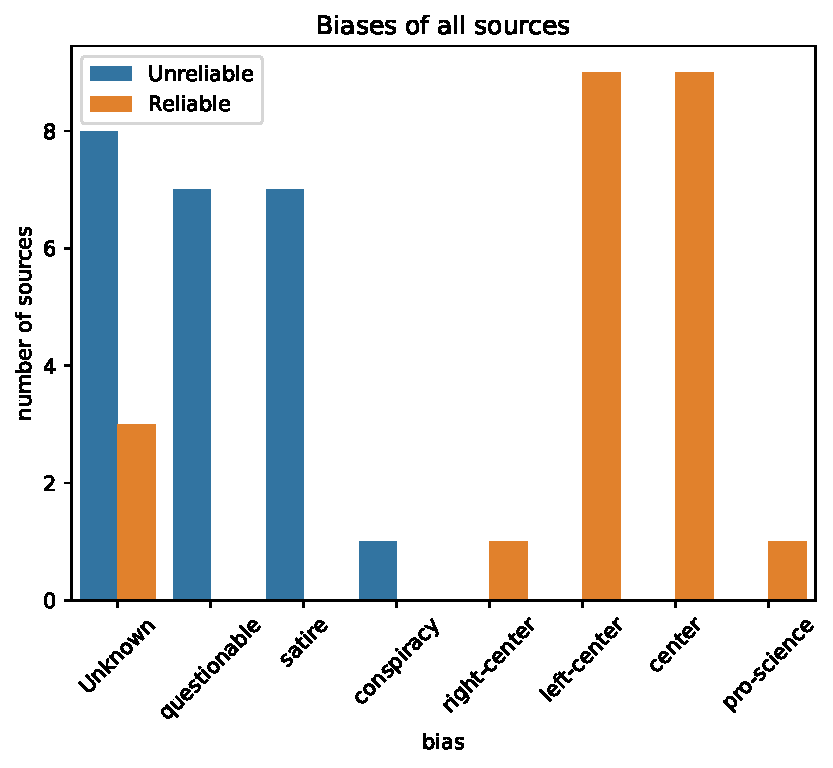
\includegraphics[width=\linewidth]{obrazky-figures/test_dataset_bias_all.pdf}
      \caption{}
      \label{fig:test_dataset_biases}
    \end{subfigure}%
    \begin{subfigure}{.5\textwidth}
      \centering
      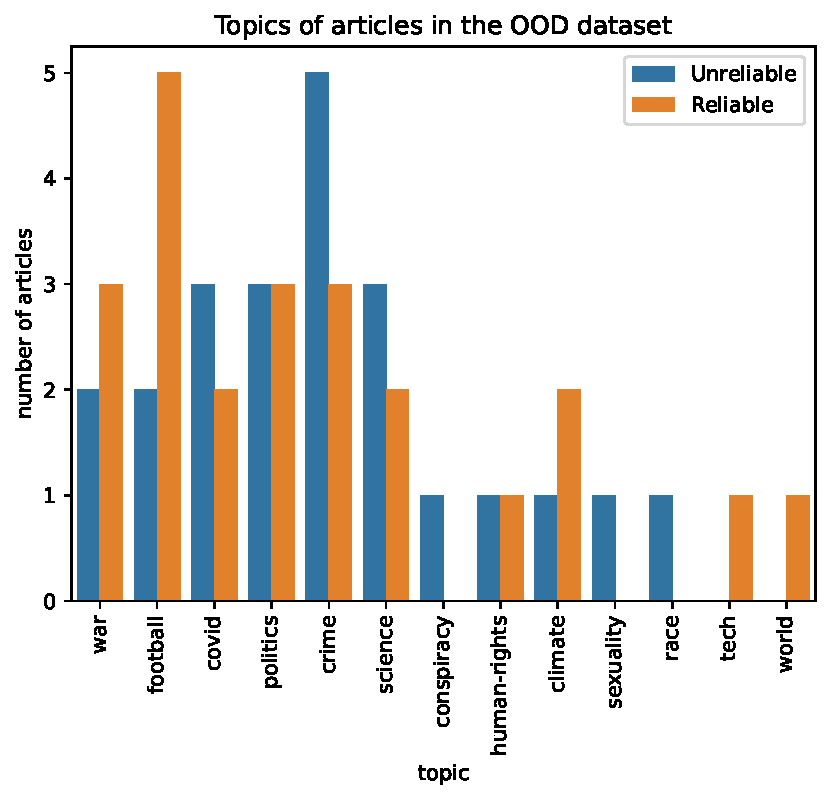
\includegraphics[width=\linewidth]{obrazky-figures/test_dataset_topics.pdf}
      \caption{}
      \label{fig:test_dataset_topics}
    \end{subfigure}
    \caption{Figure (a) shows the number of articles per bias in the FNI dataset. Figure (b) shows the topics of articles in the FNI dataset.}
    \label{fig:test4}
\end{figure}

% The factuality of a source indicates how much are the articles published by this source based on truth. It is a score ranging from 0 (least factual) to 5 (most factual). It is therefore evident, that the articles labelled as fake were published by sources with low factuality and the sources publishing articles labelled as true possess higher factuality scores.

\begin{figure}[]
    \centering
    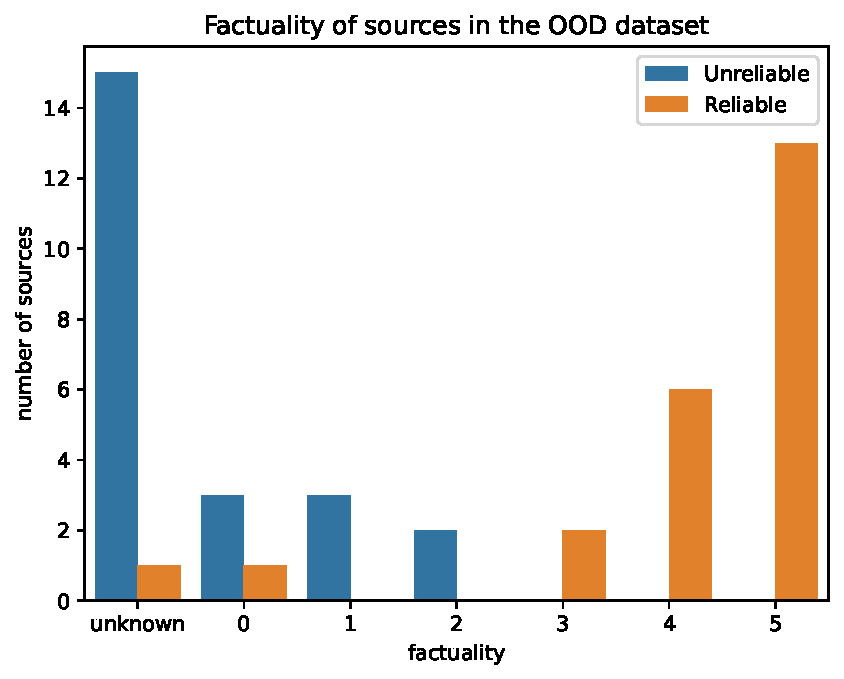
\includegraphics[scale=0.6]{obrazky-figures/test_dataset_factuality.pdf}
    \caption{Number of articles per factuality score in the FNI dataset.}
    \label{fig:test_dataset_fact}
\end{figure}


%%%%%%%%%%%%%%%%%%%%%%%%%%%%%%%%%%
% Proposed Methods
\chapter{Proposed Methods for the Classifiers}
\label{proposed-methods}
This chapter describes the methods used to create the fake news classifiers and obtain predictions in this thesis. In total two different classifiers were created. The first classifier represents the baseline model and is based on a Multinomial Naive Bayes classifier. The second classifier is based on the BERT transformer model and is meant to help better understand the clues exploited in the articles.


\section{Baseline Classifier}
\label{baseline}
The baseline classifier is based on an approach using Term Frequency-Inverse Document Frequency (TF-IDF) and Multinomial Naive Bayes Classifier. This section explains both these methods and describes how they were used in the classifier. Figure \ref{fig:baseline_model} shows the steps in the baseline model. The first step is applying some preprocessing to the input data (news articles). The preprocessing includes removing stop words, URLs and HTML code. Stop words are common words that are considered to be semantically insignificant. Examples of stop words are, e.g., “the”, “a”, “and”, etc. After the preprocessing, TF-IDF is applied to create a feature vector expected as the input for the Multinomial Naive Bayes (MNB) classifier. The MNB classifier then computes the predicted probabilities for each class, i.e., classes reliable and unreliable.

\begin{figure}[H]
    \centering
    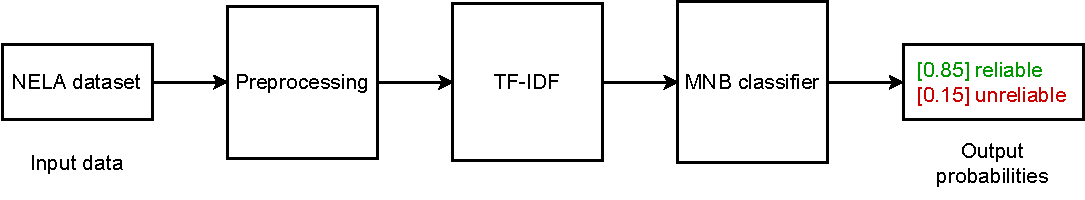
\includegraphics[scale=0.8]{obrazky-figures/baseline_model2.pdf}
    \caption{Steps of the baseline model.}
    \label{fig:baseline_model}
\end{figure}


\subsection*{TF-IDF}
As described in \cite{tf-idf}, TF-IDF is a statistic designed to reflect the importance of a term to a document in a collection of documents (also known as a corpus). It is often used for information retrieval tasks, data mining, recommender systems, as a weighting factor in search engines and other NLP tasks.
The TF-IDF value of a term for a document ranges from 0 to 1. It increases proportionally with the number of times the term appears in the document and decreases with the number of documents in which the term appeared. The computation of TF-IDF is divided into two metrics: Term frequency and Inverse document frequency.

The term frequency of a term represents the significance of the term to a document by the number of its occurrences. The first form of term weighting appeared in \cite{tf}. Term frequency of term $t$ within document $d$ is defined as:

\begin{equation}    
     \operatorname{tf}(t, d) = \displaystyle{\frac{f_{t,d}}{\sum_{t' \in d} f_{t', d}}}
\end{equation}

where $f_{t,d}$ is the number of times term $t$ occurs in document $d$ and the denominator represents the total number of terms in document $d$.

Inverse document frequency, described in \cite{idf}, is a measure of how much information a term provides to a certain document given a corpus of documents. If the term is rare and only appears in one document it is significant for the document. If the term is very common and appears in all documents, its significance and its inverse document frequency are very low. The inverse document frequency of term $t$ to a document $d$ in a corpus of documents $D$ is defined as:

\begin{equation}
     \operatorname{idf}(t, D) =  \operatorname{log} \displaystyle{\frac{N}{|\{d \in D : t \in d\}|}}
\end{equation}

where $N$ is the total number of documents in corpus $D$ meaning $|D| = N$ and the denominator is the number of documents where term $t$ appears. The denominator is often adjusted to $1 + |\{d \in D : t \in d\}|$ to avoid zero division. Finally, the TF-IDF of term $t$ is computed as the product of the two:

\begin{equation}    
     \operatorname{tfidf}(t, d, D) =  \operatorname{tf}(t,d) \cdot  \operatorname{idf}(t, D)
\end{equation}

where $d$ is a document and $D$ is the corpus of documents. The second method used in the baseline system is the Naive Bayes Classifier.

\subsection*{Multinomial Naive Bayes Classifier}
A Naive Bayes Classifier, as described in \cite{bayes} and \cite{bayes-theorem}, is a probabilistic machine learning model for classification tasks. The classifier is based on the Bayes theorem. The Bayes theorem defines the probability of an event based on prior knowledge of conditions that might be related to the event. The theorem is defined by the following equation:

\begin{equation}    
    P(a | b) = \displaystyle{\frac{P(b|a) \cdot P(a)}{P(b)}}
\end{equation}

where $a$, $b$ are realizations of events $A$, $B$ and the probability of $b$ is non-zero: $P(b) \neq 0$. The~following probabilities are used in the theorem:

\begin{itemize}
    \item $P(a | b)$ is the probability of $a$ occurring given that $b$ has occurred (so-called posterior probability in the Bayes formula).
    \item $P(b | a)$ is the conditional probability of $b$ occurring given that $a$ has occurred (so-called likelihood probability in the Bayes formula). 
    \item $P(a)$ is the probability of $a$ occurring (called the prior probability in the Bayes formula).
    \item $P(b)$ is the probability of $b$ occurring (called the evidence or marginal probability in the Bayes formula).
\end{itemize}

Using the explanation given in \cite{colins-mnb} and \cite{naive-bayes-towards}, the Naive Bayes model can be formulated as follows. The classifier uses a labelled training dataset $(\Vec{x}^{(i)}, y^{(i)})$ for $i = 1…n$, where $n$ is the number of samples in the dataset. Each $\Vec{x}^{(i)}$ is a $d$-dimensional vector, where $d$ specifies the number of features in the~model and each $y^{(i)}$ is in $\{1,2,...,k\}$, where $k$ is the number of classes in the problem. In the case of a binary classifier $k = 2$. 
Considering the problem of classifying fake news articles into two different classes (reliable, unreliable) the Multinomial Naive Bayes classifier is used. The label $y^{(i)}$ represents the class of the $i$-th article in the training set. With the approach of using word counts (or TF-IDF), $d$ corresponds to the vocabulary size in the corpus --- the total number of unique words in the dataset. Each component of the vector of features $\Vec{x}^{(i)}_j$ for $j = 1…d$, contains a number that represents the number of occurrences (or the TF-IDF value) of the $j$-th word in the $i$-th article. 

The Naive Bayes classifier assumes the features in the model are independent. That means the presence of one particular feature does not affect the other features. Hence it is called naive. Another assumption made by the model is that all the features have an equal effect on the outcome. This means they all affect the result equally. The Naive Bayes model is then derived as follows. 

\begin{equation}
    P(y | \Vec{x}) = \displaystyle{\frac{P(\Vec{x}|y) \cdot P(y)}{P(\Vec{x})}}
\end{equation}

where $y$ corresponds to the label $y^{(i)}$ and $\Vec{x}$ corresponds to the feature vector $\Vec{x}^{(i)}$. As the model assumes that all features are independent, the probability $P(\Vec{x}|y)$ can be computed as the product of the separate probabilities for each feature.

\begin{equation}    
    P(y | x_1, ..., x_d) = \displaystyle{\frac{P(x_1|y) P(x_2|y) ... P(x_d|y) P(y)}{P(x_1) P(x_2)...P(x_d)}}
    \label{eq:mnb1}
\end{equation}

where $d$ is the number of features in the model. For all entries in the dataset, the denominator does not change, it remains static. Therefore, the equation \ref{eq:mnb1} can be reformulated using proportionality.

\begin{equation}
    P(y|x_1, ..., x_d) \propto P(y) \prod_{j=1}^d P(x_j|y)
\end{equation}

In the case of a binary fake news classifier, the class variable $y$ has only two outcomes. The classification is then performed by finding the class with the maximum probability.

\begin{equation}    
    y = \underset{y\in\{1,..,k\}}{\arg\max} \; P(y) \prod_{j=1}^d P(x_j|y)
\end{equation}

where $k=2$ for a binary classifier. The probabilities in the equation are estimated from the data using the maximum-likelihood estimates for the Naive Bayes model. The probability $P(y)$ can be interpreted as the probability of seeing the label y in the data. The maximum-likelihood estimates for $P(y)$, where $y \in {1…k}$ take the following form.

\begin{equation}
    P(y) = \displaystyle{\frac{\sum_{i=1}^n \mathbb{I}[y^{(i)} = y]}{n} = \frac{\operatorname{count}(y)}{n}}
    \label{eq:ml1}
\end{equation}

where $n$ is the number of samples (articles) in the dataset and $\mathbb{I}[y^{(i)} = y]$ is defined as $1$ if $y^{(i)} = y$, $0$ otherwise. Therefore, $\sum_{i=1}^n \mathbb{I}[y^{(i)} = y]$ corresponds to the number of times label $y$ appears in the dataset. As the equation \ref{eq:ml1} shows, the probability of $P(y)$ is simply the number of times the label $y$ appears in the dataset divided by the number of samples in the dataset. 

The other probability that needs to be estimated is the $P(x_j|y)$ for each feature $j \in d$ in vector $\Vec{x}$. This probability can be understood as the probability of feature $x_j$ appearing in a sample belonging to class $y$. The ML estimates for $P(x_j|y)$ depend on the distribution of the training data. In the case of a Multinomial Naive Bayes classifier, the ML estimates take the following form.

\begin{equation}
    P(x_j|y) = \displaystyle{\frac{\sum_{i=1}^n \mathbb{I}[y^{(i)} = y] \; x_j^{(i)}}{\sum_{i=1}^n \sum_{t=1}^d \mathbb{I}[y^{(i)} = y] \; x_t^{(i)}} = \frac{\operatorname{N}_{yj}}{\operatorname{N}_y}}
    \label{eq:ml2}
\end{equation}

where $n$ is the number of samples in the dataset, $\operatorname{N}_{yj}$ is the is the number of times feature $j$ appears in a sample of class $y$ in the training dataset and $\operatorname{N}_y$ is the total count of all features for class $y$. In the case of using TF-IDF values the equation just sums the TF-IDF values of features instead of the discrete counts of their occurrence. The equation \ref{eq:ml2} is often adjusted by adding a smoothing prior $\alpha \geq 0$. The smoothing accounts for features not present in the training samples and prevents zero probabilities in the computation. Setting $\alpha = 1$ is called Laplace smoothing and when $\alpha < 1$ it is called the Lidstone smoothing. 

\begin{equation}
    P(x_j|y) = \displaystyle{\frac{N_{yj} + \alpha}{N_y + \alpha d}}
    \label{eq:ml_estimates}
\end{equation}

where $d$ is the number of features in the model. During the inference of new articles, the new TF-IDF values of these articles are used as an exponent of the trained probabilities as described in equation \ref{eq:infer-prob}.

\begin{equation}
    P(y|\Vec{x}) = \displaystyle{\frac{P^{'}(\Vec{x}|y) \cdot P(y)}{\sum_y{P^{'}(\Vec{x}|y) \cdot P(y)}}}
    \label{eq:infer-prob}
\end{equation}

where $P^{'}$ is the distribution exponentiated by the new TF-IDF values. The Multinomial Naive Bayes classifier is intended to be used with integer feature (word) counts. However, TF-IDF vectors are also known to work well in practice. Both approaches --- the word counts and TF-IDF vectors --- were tried and compared in this thesis and the approach of using TF-IDF was found to perform slightly better. This comparison is further described in chapter \ref{experiments}. 

In this thesis, the scikit-learn\footnote{\url{https://scikit-learn.org/stable/modules/naive_bayes.html\#multinomial-naive-bayes}} implementation of the MNB classifier is used. This implementation uses the formula described in equation \ref{eq:ml_estimates} to compute the ML estimates.
Among the advantages of a Naive Bayes Classifier is the speed of computation and ease of implementation. The disadvantage of this model is the fact that all features are considered independent. In reality, words have relations with each other and are often part of a broader context. To solve these problems the BERT transformer model is proposed in the next section. 


%on the other hand, include the equality of features (meaning all features influence the outcome of the classifier equally)




\section{BERT Classifier}
\label{sec:bert}
This section describes the second classifier implemented in this thesis. The architecture chosen for the second classifier is the BERT model. The baseline classifier models the documents based only on the occurrence of words without any deeper understanding of the text. A~better approach is using word embeddings that are trained to capture the relationships between words based on their co-occurrence in a document and convey the meaning of words to allow for deeper understanding. The BERT model uses contextualized embeddings where the embedding of a word depends on the context of the sentence in which it occurs.
The BERT (Bidirectional Encoder Representations from Transformers) model, introduced in \cite{bert}, is a language representation model that produces state-of-the-art results in a wide variety of NLP tasks. The model utilizes the approach of transfer learning --- pre-training a neural network model and fine-tuning it for specific tasks. This means BERT was designed to pre-train deep bidirectional representations from unlabeled text and then fine-tune the pre-trained model on a downstream task. During the fine-tuning, the model is first initialized with the pre-trained parameters. All parameters are then fine-tuned using labelled data, e.g., by adding one additional output layer to the model.
The architecture of BERT is based on the Transformer architecture described in \cite{transformer}. The Transformer architecture uses the encoder-decored structure displayed in figure \ref{fig:transformer}.

\begin{figure}[H]
    \centering
    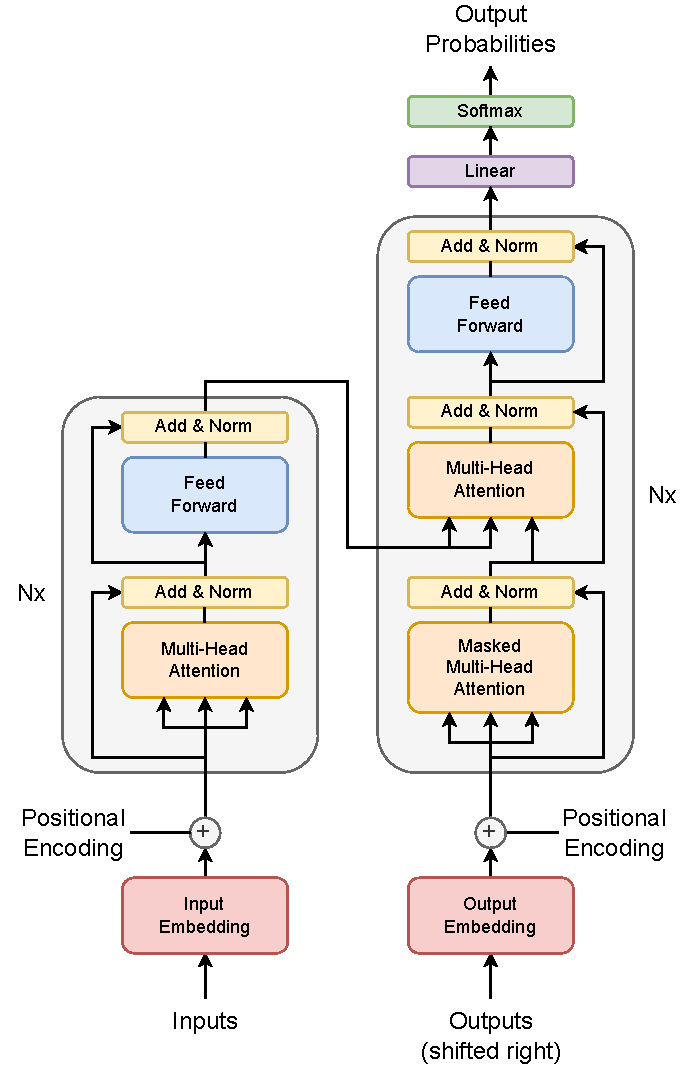
\includegraphics[scale=0.7]{obrazky-figures/transformer.pdf}
    \caption{Architecture of the Transformer model, as described in \cite{transformer}.}
    \label{fig:transformer}
\end{figure}

The encoder takes an input sequence (e.g., a sentence in English) and computes its hidden representation. This hidden representation is then used by the decoder to generate the desired output sequence of symbols one element at a time (e.g., the input sentence translated to French). As the decoder generates the output it uses the previously generated symbols as additional input when generating the next symbol. This transformation of an input sequence to an output sequence makes the model suitable for applications like translation, question answering, text summarization, etc.

Each word in the input sentence is first transformed into the input embedding 512-dimensional vector, to which positional encoding is added. The positional encoding is a vector that helps to determine the position of words in the sentence. After that the vectors are passed into the first layer of the encoder. The original paper uses a stack of $N=6$ layers in the encoder connected in a sequence. Each layer contains two components: a multi-head self-attention mechanism and a feed-forward neural network.

\subsection*{Multi-head Attention}
The self-attention mechanism helps the model determine the relevance between words in the input sentence. As the model processes each word, the self-attention allows it to look at the other words and based on their relevance to the processed word contribute to a better encoding for this word. For example, when the model processes this sentence: “The animal didn't cross the street because it was too tired”, self-attention allows the model to associate the word “it” with the word “animal”.

The self-attention mechanism works as follows. First, each input vector of the encoder (the word embeddings in the first layer) is transformed into three vectors: Query vector $q$ and Key vector $k$ of dimensions $d_k$, and Value vector $v$ of dimension $d_v$. These vectors are created by multiplying the input embedding with three weight matrices $W_Q$, $W_K$, and $W_V$ that are trained during the training process, as displayed in figure \ref{fig:attention1}.

\begin{figure}[H]
    \centering
    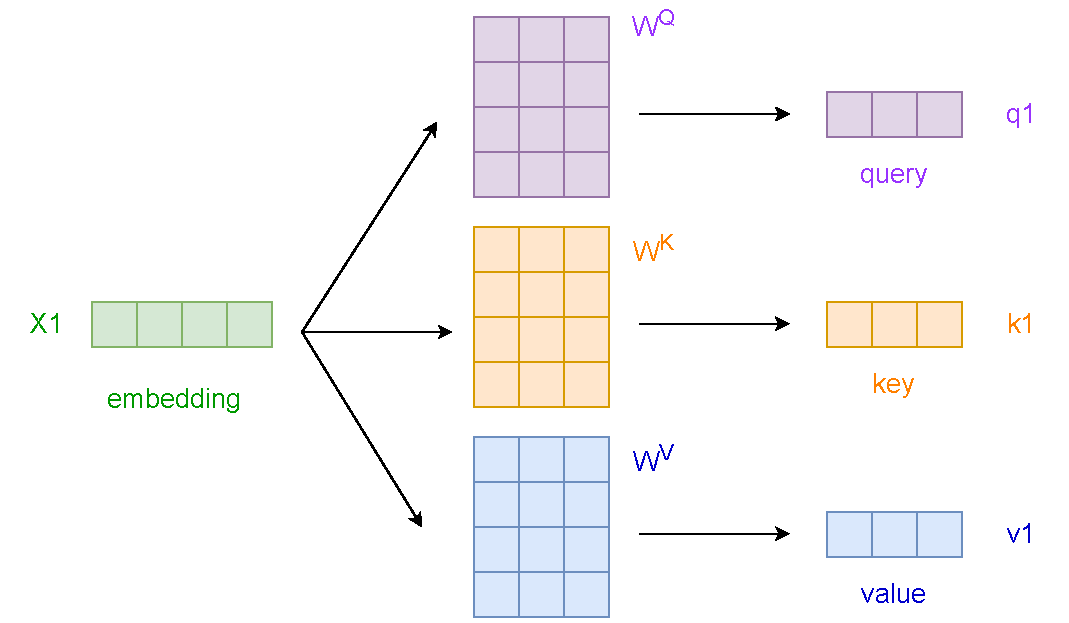
\includegraphics[scale=0.6]{obrazky-figures/attention1.pdf}
    \caption{Creation of the query, key and value vectors from the input embedding by multiplying the embedding with weight matrices trained during the training process (biases omitted for simplicity).}
    \label{fig:attention1}
\end{figure}


To compute the attention vector for a word at position $i=1$ with all the other words $j\in1...t$ where $t$ is the number of words in the sentence, the model computes the dot product of query $q_i$ with each key $k_j$, divides the result by $\sqrt{d_k}$ and applies the $\operatorname{softmax}$ function to obtain the weights of the values. After that, each value vector $v_j$ is multiplied by the corresponding $\operatorname{softmax}$ value to obtain a weighted value vector. In the last step, all the weighted value vectors are summed to create one attention vector $z_i$ for word $i$. This process is shown in figure \ref{fig:attention2}.

\begin{figure}[H]
    \centering
    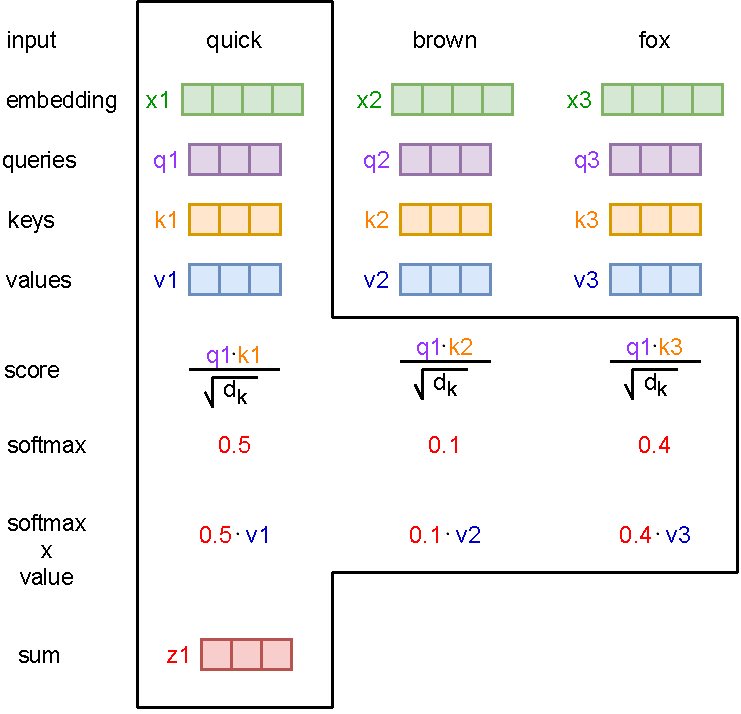
\includegraphics[scale=0.8]{obrazky-figures/attention2.pdf}
    \caption{Computation of the attention vector $z$ for a word in a sequence, as described in The Illustrated Transformer \cite{illustrated-transformer}.}
    \label{fig:attention2}
\end{figure}


In practice, the input vectors, their queries, keys and values are all packed together into matrices and the attention function is computed for a set of queries simultaneously. The attention of a query matrix $Q \in \mathbb{R}^{L \times d_k}$, a key matrix $K \in \mathbb{R}^{L \times d_k}$ and a value matrix $V \in \mathbb{R}^{L \times d_v}$ --- where $d_k$ is the dimension of the query and key vectors and $d_v$ is the dimension of the value vector --- can be represented by equation \ref{eq:attention}.

\begin{equation}
    \operatorname{Attention}(Q, K, V) = \operatorname{softmax} \displaystyle{(\frac{QK^T}{\sqrt{d_k}})V}
    \label{eq:attention}
\end{equation}

where $d_k$ is the dimension of the query and key vectors (64 in the original paper). The process described above is the computation of a single attention function. The Transformer model uses Multiple-head attention. Each attention head contains its own weight matrices $W_Q$, $W_K$, $W_V$ and computes the attention matrix $Z_i$. The matrices from all heads are then concatenated together and multiplied by another weight matrix $W^0$ trained jointly with the model. After that, the flow continues to the second component of the transformer --- a feed-forward neural network --- which is applied to every one of the attention vectors. Around each of the components, there is a residual connection followed by layer normalization. 

The decoder is also composed of $N=6$ identical layers. The input for the decoder is actually the desired output of the transformer (e.g., a sentence translated into another language). The BERT model uses only the encoder, therefore, the decoder is not further described in this section.
% The output is first transformed into embeddings and positional encoding is added. After that masked multi-head self-attention is applied. In this case, the self-attention just masks the words that follow later in the sequence which ensures that the prediction for position $i$ depends only on the known words that came before $i$. After that another multi-head self-attention is applied, this time combining the outputs of the encoder with the decoder. This is where the mapping between English and French words (in the example of language translation) takes place. The last component of the decoder is once again a feed-forward neural network. The decoder employs residual connections and normalization just like the encoder. Finally, after a linear layer followed by softmax, the transformer generates the output probabilities.

\subsection*{BERT model}
The BERT model used in this thesis is based on the Transformer described above. The architecture of BERT is a multi-layer bidirectional Transformer encoder as it uses only the encoder part of the transformer. Authors of the BERT model created two pre-trained versions: $\operatorname{BERT_{BASE}}$ and $\operatorname{BERT_{LARGE}}$. The $\operatorname{{BERT_{BASE}}}$ model used in this thesis contains 12 encoder blocks and 110 million parameters.
The BERT model is pre-trained on two unsupervised tasks: Masked Language Model (MLM) and Next Sentence Prediction (NSP).

MLM is used to train bidirectional representations. A percentage of the input tokes is masked at random --- they are replaced by the [MASK] token. The model then learns to predict the masked words from the context words on either side of the sequence. This is achieved by adding a classification layer at the end of the encoder and performing a softmax over the vocabulary. A downside to this approach is that the [MASK] token is not used during fine-tuning. Therefore the [MASK] token is only used in 80\% of the randomly selected tokens, 10\% is replaced by a random token and the remaining 10\% stays unchanged. During the training, a cross-entropy loss is used.

In NSP the model is fed pairs of sentences $A$, $B$ and learns to predict whether sentence $B$ is subsequent to sentence $A$ in the original document. In 50\% of the pairs used for training, $B$ is subsequent to $A$ and in the other 50\%, $B$ is a random sentence not subsequent to sentence $A$. Both sentences are fed into the model as one input sequence. Each sequence starts with the [CLS] token, followed by tokens of sentences $A$ and $B$ separated by the [SEP] token. The model then takes the token embeddings of each word and adds a segment embedding, indicating to which sentence the given word corresponds, and a position embedding, that indicates the position of each word in the sequence. Figure \ref{fig:bert1} provides a visual illustration of the BERT input representation.

\begin{figure}[H]
    \centering
    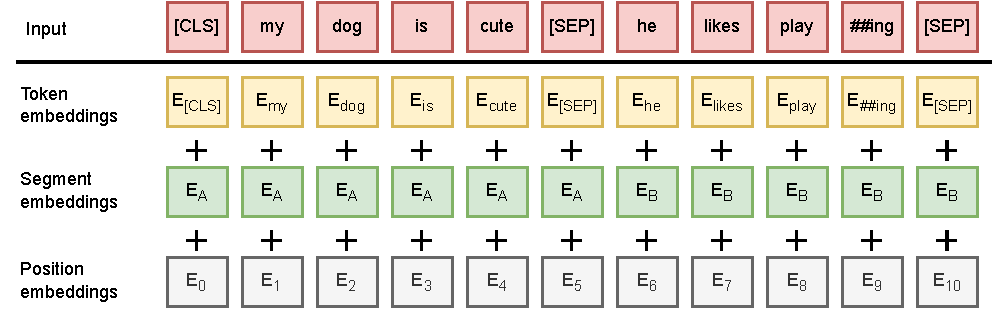
\includegraphics[scale=0.8]{obrazky-figures/bert1.pdf}
    \caption{Representation of BERT input is the sum of token embeddings, segmentation embeddings and position embeddings, as described in \cite{bert}.}
    \label{fig:bert1}
\end{figure}

When training the model the MLM and NSP are trained together. To predict whether the sentence $B$ is subsequent to $A$ the model adds a classification layer on top of the encoder output for the [CLS] token and computes the probability with softmax.

This thesis uses the $\operatorname{{BERT_{BASE}}}$ uncased model that was pre-trained on the BooksCorpus (800M words) \cite{book_corpus} and English Wikipedia (2,500M words). The model is then fine-tuned on the NELA dataset described in section \ref{nela-my}, which contains binary labels representing whether the given article is reliable or unreliable. For fine-tuning, a classification layer is added on top of the encoder output for the [CLS] token. The classification layer is simply a linear layer with dropout and optionally some activation function, e.g., ReLU. The linear layer has 768 input features (hidden size of $\operatorname{{BERT_{BASE}}}$) and 2 output features (number of labels in the dataset). The fine-tuning process is displayed in figure \ref{fig:bert2}.

\begin{figure}[H]
    \centering
    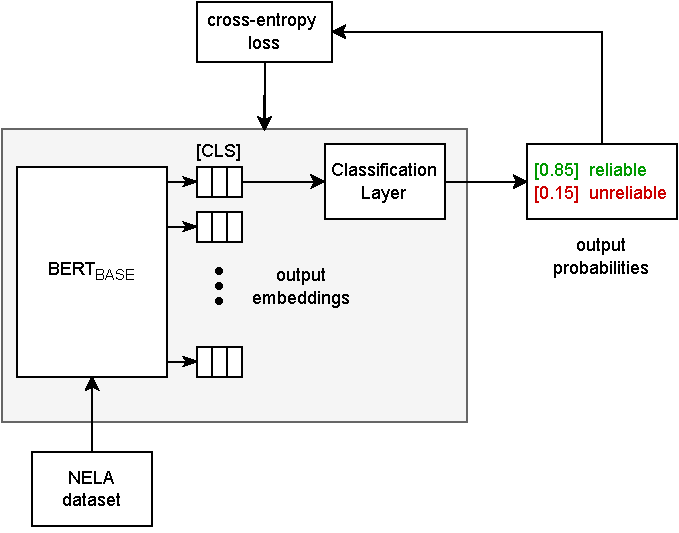
\includegraphics[scale=0.9]{obrazky-figures/bert2.pdf}
    \caption{Fine-tuning the $\operatorname{BERT_{BASE}}$ model on the NELA dataset.}
    \label{fig:bert2}
\end{figure}



\section{Interpretability with Integrated Gradients}
\label{sec:integ_grads}
This section describes the method used for gaining interpretable cues from the BERT classifier. Due to the deep stack of layers used in models like BERT, deep neural networks are often viewed as black boxes in the sense that it is not simple to interpret the predictions they generate. However, it is possible to implement a method able to interpret the predictions of neural networks. An interpretation method like this seeks to answer the following questions: (i) Why does the model predict the given class? (ii) What are the features exploited by the model during the prediction (i.e., what are the most important words that influence the prediction)?

To gain interpretable cues from the BERT classifier the Integrated gradients (IG) method is used in this thesis. Integrated gradients, presented in \cite{integ_grads}, is a method that requires no modification to the original network. It is simple to implement and can be applied to any deep-learning model for classification and regression tasks. The method computes an attribution score for each input feature of the deep learning model based on the gradients of the output prediction. Following is the formal definition of the method, as defined in \cite{integ_grads}.

\vspace{2mm}

\textbf{Definition:} Suppose a function $F: \mathbb{R}^n \rightarrow [0, 1]$ that represents a deep network and a~vector $\Vec{x} = (x_1, …, x_n)$ representing an input. An attribution of the prediction at input $\Vec{x} \in \mathbb{R}^n$ relative to a baseline input $\Vec{x}^{'} \in \mathbb{R}^n$ is a vector $\Vec{a}_F(\Vec{x}, \Vec{x}^{'}) = (a_1, …, a_n) \in \mathbb{R}^n$ where each $a_i$ is the contribution of $x_i$ to the prediction for $F(\Vec{x})$.

\vspace{2mm}

The vector $\Vec{x}$ is used as the input of the neural network for simplicity as usually the input of a neural network is a matrix. The Integrated gradients method requires two sets of input: the original input and a baseline input. The original input corresponds to the unchanged input $\Vec{x}$ of the network. The baseline input is constructed from the original input and should contain neutral values. As suggested by the authors of the original paper, for image processing, the baseline could be a black image, whereas for text models it could be a zero embedding vector. In practice, the [PAD] token is often used in the baseline input, as it is interpreted by the network as empty space (even though it does not have zero embeddings). The difference between the original and baseline input is also described in figure \ref{fig:integ_grads1}.

\begin{figure}[H]
    \centering
    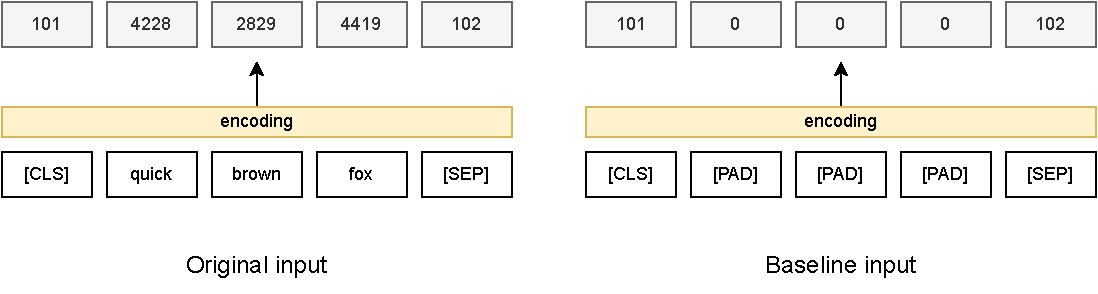
\includegraphics[scale=0.8]{obrazky-figures/integ_grads1.pdf}
    \caption{Example of the input and baseline text used in the Integrated gradients method as described in \cite{integ_grads_towards}.}
    \label{fig:integ_grads1}
\end{figure}

The Integrated gradients are defined as the integral of the gradients along a straight line path (in $\mathbb{R}^n$) from the baseline $\Vec{x}^{'}$ to the original input $\Vec{x}$. The Integrated gradient of the $i^{th}$ dimension for an input $\Vec{x}$ and a baseline input $\Vec{x}^{'}$ is defined in equation \ref{eq:integ_grads1}.

\begin{equation}
    \operatorname{IntegratedGrads}_i(\Vec{x}) = (x_i - x^{'}_i) \cdot \int_{\alpha = 0}^{1} \displaystyle{\frac{\partial F(\Vec{x}^{'} + \alpha \cdot (\Vec{x}-\Vec{x}^{'}))}{\partial x_i}} d\alpha
    \label{eq:integ_grads1}
\end{equation}

where $\frac{\partial F(\Vec{x})}{\partial x_i}$ is the gradient of $F(\Vec{x})$ along the $i^{th}$ dimension. In practice, the integral of Integrated gradients can be approximated as the sum of the gradients at multiple points occurring at sufficiently small intervals on the straight line between $\Vec{x}^{'}$ and $\Vec{x}$. This technique is also known as the Riemann sum. It is the sum of the gradients divided by the number of approximation steps. Equation \ref{eq:integ_grads1} can be therefore approximated as:

\begin{equation}
    \operatorname{IntegratedGrads}^{approx}_i(\Vec{x}) = (x_i - x^{'}_i) \cdot \sum_{k=1}^{m} \displaystyle{\frac{\partial F(\Vec{x}^{'} + \frac{k}{m} \cdot (\Vec{x} - \Vec{x}^{'}))}{\partial x_i}} \cdot \frac{1}{m}
    \label{eq:integ_grads2}
\end{equation}

where $m$ is the number of approximation steps. In the case of the BERT classifier used in this thesis, function $F$ represents the classifier model. The model predicts the probabilities of two classes, therefore one target probability, e.g., probability of class \texttt{reliable}, is selected to be the output of $F$. The input $\Vec{x}$ represents the text of an article and $x_i$ represents each word. The IG method gradually interpolates the baseline input $\Vec{x}^{'}$ to move closer to the original input --- by increasing the $k$ value in each approximation step --- and feeds it into the network. This is achieved by the following part of the equation: $(\Vec{x}^{'} + \frac{k}{m} \cdot (\Vec{x} - \Vec{x}^{'}))$.
In the last step when $k=m$ the interpolated input is identical to the original input. The interpolated inputs are gradually fed into the network and in each step, the gradient of $F$ along the $i^{th}$ dimension is computed. 
The formula computes the attribution score for each embedding element. The BERT classifier used in this thesis uses 768-dimensional embeddings. Therefore the final attribution score of the $i^{th}$ word is computed as the attribution average of all of the embedding elements. The attribution score is computed for all words in the text as displayed in figure \ref{fig:integ_grads2}.

\begin{figure}[H]
    \centering
    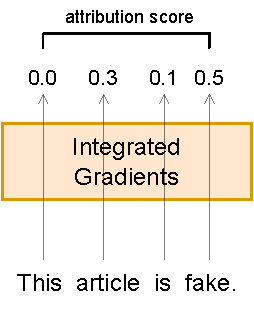
\includegraphics[scale=1]{obrazky-figures/ig.pdf}
    \caption{Application of Integrated gradients as described in \cite{integ_grads_towards}.}
    \label{fig:integ_grads2}
\end{figure}

The method of Integrated gradients is used to get an insight into the predictions of the BERT classifier and explore which features of the text are exploited by the model when making predictions. Chapter \ref{chap:inter_anal} describes the qualitative analysis of the created classifiers using the IG method.


%%%%%%%%%%%%%%%%%%%%%%%%%%%%%%%%%%
% Technical Details
\section{Technical Details}
\label{implementation}
This section provides a brief discussion of the tools and libraries used to implement the models in this thesis. All models are implemented in Python 3.9.7. The implementation of the baseline model uses the Python scikit-learn\footnote{\url{https://scikit-learn.org/stable/}} library. Two main classes are used by the baseline. The TfidfVectorizer is used to convert a collection of input articles to a matrix of TF-IDF features. The MultinomialNB class is an implementation of the Naive Bayes classifier for multinomial models and is used as the classifier in the baseline. Both classes can be found on the scikit-learn website. 

The BERT classifier uses the Hugging Face framework. In particular the pre-trained BERT base uncased model\footnote{\url{https://huggingface.co/bert-base-uncased}}. For the implementation of Integrated gradients, the Layer Integrated Gradients\footnote{\url{https://captum.ai/api/layer.html\#layer-integrated-gradients}} class from the Captum library is used. The usage of this class is based on an explanation in \cite{integ_grads_towards}.





%%%%%%%%%%%%%%%%%%%%%%%%%%%%%%%%%%
% Experiments
\chapter{Quantitative Analysis of the Classifiers}
\label{experiments}
This chapter summarizes the quantitative evaluation of the classifiers implemented in this thesis. The intention is to evaluate the performance of the Baseline classifier and the BERT classifier by applying various evaluation metrics and to analyse their biases in certain areas. To test the implemented classifiers, the following evaluation process was used:

\begin{enumerate}
    \item Train the classifier on a split of the NELA dataset (train set).
    \item Tune the hyper-parameters of the model using the validation split of the NELA dataset (validation set).
    \item Evaluate the classifier on the test split of the NELA dataset (test set).
    \item Perform cross-evaluation of the classifier on the Merged dataset.
    \item Perform cross-evaluation of the classifier on the FNI dataset.
\end{enumerate}

The evaluation of the classifiers is performed using four evaluation metrics: accuracy, precision, recall and F1-score. Following is a brief explanation of these methods.

\subsection*{Confusion Matrix}
To understand the evaluation metrics it is first important to introduce the confusion matrix. A confusion matrix as described in \cite{confusion_matrix}, is a square matrix that is used to evaluate the performance of machine learning algorithms in classification tasks. Each row of the matrix represents the instances in the actual class while each column represents the instances predicted by the model.

\begin{figure}[H]
    \centering
    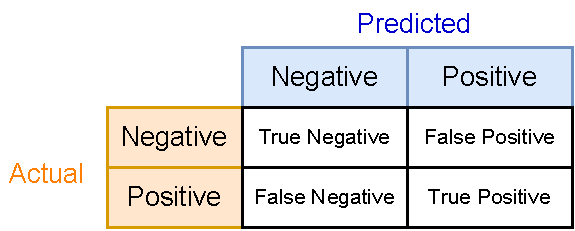
\includegraphics[scale=0.9]{obrazky-figures/conf_mat2.pdf}
    \caption{Example of a confusion matrix for a binary classifier.}
    \label{fig:conf_mat}
\end{figure}

In the case of a binary classifier with only two classes (negative and positive), the confusion matrix would look as displayed in figure \ref{fig:conf_mat}.
The numbers in the cells have specific names. True negative (TN) is the number of instances of class negative that were correctly predicted as negative. False negative (FN) is the number of instances of class positive that were mistakenly classified as negative. False positive (FP) is the number of negative instances falsely predicted to be positive. True positive (TP) is the number of instances correctly classified as positive.


\subsection*{Accuracy}
Accuracy is defined as the number of correctly predicted instances divided by the total number of instances in the dataset (confusion matrix). Using the terms of the confusion matrix it could be also defined as:

\begin{equation}
    Accuracy = \displaystyle{\frac{TN + TP}{TN + FP + TP + FN}}
\end{equation}

Accuracy is often used together with other metrics --- precision and recall --- to better reflect the capabilities of the classifier.

\subsection*{Precision}
Precision is defined as the number of correctly predicted instances of one class divided by the total number of predictions of that class. Equation \ref{eq:precision} shows the definition in terms of the confusion matrix for class positive.

\begin{equation}
    \label{eq:precision}
    Precision = \displaystyle{\frac{TP}{TP + FP}}
\end{equation}

Precision is a good measure to determine the performance of a model where the cost of a false positive (FP) is high. For example, in a fake news classifier, the positive class could be interpreted as fake news and the negative as true (not fake news). In that case, a false positive would be a non-fake news article falsely classified as fake news. A model with too many false positives would receive a low precision.


\subsection*{Recall}
Recall is defined as the number of correctly predicted instances of one class divided by the total number of actual instances of that class, as displayed in equation \ref{eq:recall}.

\begin{equation}
    \label{eq:recall}
    Recall = \displaystyle{\frac{TP}{TP + FN}}
\end{equation}

Recall is crucial for models with a big risk associated with false negatives (FN). In the case of a fake news classifier, false negatives would be fake news articles that are falsely classified as true. In this case, the cost of such a prediction may be harmful but not catastrophic. But for a classifier predicting whether a bank transaction is fraudulent, the consequence of false negative cases could be very bad for the bank.

\subsection*{F1-score}
F1-score is a function of precision and recall. It is defined using the following formula.

\begin{equation}
    F1 = 2 \cdot \displaystyle{\frac{Precision \cdot Recall}{Precision + Recall}}
\end{equation}

The F1 score is beneficial for finding a balance between precision and recall and for datasets with an uneven class distribution.



\section{Evaluation on the NELA Test Set}
\label{sec:eval_nela}
This section describes the evaluation of the baseline and BERT classifiers on the test split of the NELA  dataset. A detailed description of the NELA dataset and its preprocessing can be found in sections \ref{nela} and \ref{nela-my}. Table \ref{tab:nela_val_test} shows the number of articles in the train, test and validation splits. The distribution of labels is well-balanced with all splits having an accuracy around 50\% for majority and random classifiers.

\begin{table}[H]
    \centering
\begin{tabular}{r|r|r|r|}
\cline{2-4}
\multicolumn{1}{c|}{} & \multicolumn{1}{c|}{\textbf{Reliable}} & \multicolumn{1}{c|}{\textbf{Unreliable}} & \multicolumn{1}{c|}{\textbf{Total}} \\ \hline
\multicolumn{1}{|r|}{\textbf{Train}}      & 312,069 & 304,729 & 616,798 \\ \hline
\multicolumn{1}{|r|}{\textbf{Test}}       & 98,337  & 98,103  & 196,440 \\ \hline
\multicolumn{1}{|r|}{\textbf{Validation}} & 78,851  & 78,346  & 157,197 \\ \hline
\end{tabular}
    \caption{Number of reliable and unreliable articles in the train, test and validation splits of the NELA dataset.}
    \label{tab:nela_val_test}
\end{table}

The architecture of the baseline classifier combines the TF-IDF method with a Multinomial Naive Bayes (MNB) classifier and was described in section \ref{baseline}.
Different configurations of the baseline model were examined in order to leverage its capabilities. Multinomial Naive Bayes (MNB) is often used with just word counts instead of TF-IDF. Table \ref{tab:baseline_tf-idf} shows the comparison of using word counts and TF-IDF in the baseline classifier.
The table shows the precision, recall and F1-score for each label and the overall accuracy. As the results show, the usage of TF-IDF slightly improved the classifier. 

\begin{table}[H]
    \centering
\begin{tabular}{cc|c|c|c|}
\cline{3-5}
                                        &                     & \textbf{Precision} & \textbf{Recall} & \textbf{F1-score} \\ \hline
\multicolumn{1}{|c|}{\multirow{3}{*}{Word counts}} & \textbf{Reliable}   & 0.77               & 0.80            & 0.78              \\ \cline{2-5} 
\multicolumn{1}{|c|}{}                  & \textbf{Unreliable} & 0.80               & 0.76            & 0.78              \\ \cline{2-5} 
\multicolumn{1}{|c|}{}                  & \textbf{Accuracy}   & \multicolumn{3}{c|}{0.78}                                \\ \hline \hline
\multicolumn{1}{|c|}{\multirow{3}{*}{TF-IDF}} & \textbf{Reliable}   & 0.79               & 0.80            & 0.80              \\ \cline{2-5} 
\multicolumn{1}{|c|}{}                  & \textbf{Unreliable} & 0.80               & 0.78            & 0.79              \\ \cline{2-5} 
\multicolumn{1}{|c|}{}                  & \textbf{Accuracy}   & \multicolumn{3}{c|}{0.79}                                \\ \hline
\end{tabular}
    \caption{Comparison of using word counts and TF-IDF in the baseline classifier.}
    \label{tab:baseline_tf-idf}
\end{table}

The TF-IDF classifier achieved an accuracy of 79\%. When using the word counts, the accuracy dropped to 78\%. An improvement in the performance of the baseline was achieved when the TF-IDF values were computed using not only words (unigrams) but also bigrams and trigrams. A bigram is a sequence of two adjacent words in a sentence and a trigram is a sequence of three adjacent words. This approach improved the accuracy of the model to 86\%. Table \ref{tab:baseline_trigrams} shows the evaluation results of this approach.


\begin{table}[H]
    \centering
\begin{tabular}{c|ccc|}
\cline{2-4}
 & \multicolumn{1}{c|}{\textbf{Precision}} & \multicolumn{1}{c|}{\textbf{Recall}} & \textbf{F1-score} \\ \hline
\multicolumn{1}{|c|}{\textbf{Reliable}} & \multicolumn{1}{c|}{0.84} & \multicolumn{1}{c|}{0.89} & 0.86 \\ \hline
\multicolumn{1}{|c|}{\textbf{Unreliable}} & \multicolumn{1}{c|}{0.88} & \multicolumn{1}{c|}{0.82} & 0.85 \\ \hline
\multicolumn{1}{|c|}{\textbf{Accuracy}} & \multicolumn{3}{c|}{0.86} \\ \hline
\end{tabular}
    \caption{Baseline with TF-IDF, unigrams, bigrams and trigrams evaluated on the NELA test set.}
    \label{tab:baseline_trigrams}
\end{table}


Adding bigrams and trigrams, however, dramatically increased the memory usage of the model making it much slower. Table \ref{tab:mem_comp} compares the corpus size of the two approaches. The corpus size represents the number of features of the model. For the baseline model using only words (unigrams), the corpus size is equal to the number of all unique words in the dataset. For the model with words, bigrams and trigrams the corpus size is enlarged by the number of unique bigrams and trigrams.

\begin{table}[H]
    \centering
\begin{tabular}{|c|r|}
\hline
\textbf{Approach}           & \textbf{Corpus Size}  \\ \hline
unigrams                    & 587,587                             \\ \hline
unigrams, bigrams, trigrams & 174,785,580                         \\ \hline
\end{tabular}
    \caption{Comparison of the corpus size.}
    \label{tab:mem_comp}
\end{table}

The best performance of the baseline model was achieved using TF-IDF, unigrams, bigrams and trigrams. This approach outperformed the other approaches in all evaluation metrics. The downside of this approach is its memory usage and slow speed. The requirements for the baseline model in this thesis were to be a simple, quick solution that is not resource-heavy. Therefore, for all the remaining experiments in this thesis only the baseline model with unigrams is used.

The second classifier implemented in this thesis is based on the BERT model architecture and is described in section \ref{sec:bert}. The validation split of the NELA dataset was used to tune the hyper-parameters of the model. To find the best hyper-parameters a simple grid search was applied. The ranges of values for each parameter were suggested in the original paper \cite{bert}. The following hyper-parameters were found to be the best.

\begin{itemize}
    \item learning rate: 2e-5
    \item number of epochs: 2
\end{itemize}

The NELA dataset used for training was preprocessed by filtering certain keywords from the text, e.g., names of sources, etc. The baseline classifier was not influenced by this filtering as the results of his performance did not change. For the BERT classifier, however, the accuracy on the NELA test set dropped from 97\% to 94\% when the filtered dataset was used. The evaluation of the BERT classifier before and after keyword filtering is displayed in table \ref{tab:bert_eval1}.

\begin{table}[H]
    \centering
\begin{tabular}{cc|c|c|c|}
\cline{3-5}
                                        &                     & \textbf{Precision} & \textbf{Recall} & \textbf{F1-score} \\ \hline
\multicolumn{1}{|c|}{\multirow{3}{*}{Before kw filtering}} & \textbf{Reliable}   & 0.96               & 0.98            & 0.97              \\ \cline{2-5} 
\multicolumn{1}{|c|}{}                  & \textbf{Unreliable} & 0.98               & 0.96            & 0.97              \\ \cline{2-5} 
\multicolumn{1}{|c|}{}                  & \textbf{Accuracy}   & \multicolumn{3}{c|}{0.97}                                \\ \hline \hline
\multicolumn{1}{|c|}{\multirow{3}{*}{After kw filtering}} & \textbf{Reliable}   & 0.95               & 0.94            & 0.94              \\ \cline{2-5} 
\multicolumn{1}{|c|}{}                  & \textbf{Unreliable} & 0.94               & 0.95            & 0.94              \\ \cline{2-5} 
\multicolumn{1}{|c|}{}                  & \textbf{Accuracy}   & \multicolumn{3}{c|}{0.94}                                \\ \hline
\end{tabular}
    \caption{Evaluation of the BERT classifier before and after keyword filtering.}
    \label{tab:bert_eval1}
\end{table}

Keyword filtering was applied to prevent the classifiers from focusing on simple cues like names of sources and focus more on the semantics of the text. The model trained on the NELA dataset with keyword filtering is therefore used in all the experiments in this thesis. 
Table \ref{tab:baseline_bert_diff} shows the difference in performance between the baseline classifier using TF-IDF with unigrams and the BERT classifier. It is not surprising that the BERT classifier outperforms the baseline in every metric. The overall accuracy of the BERT model is 14\% higher than the accuracy of the baseline. The goal of this thesis, however, is not to show that the BERT model performs better than an MNB classifier. The goal is to analyse the biases and limitations of content-based methods and discover the cues exploited by these methods in the text. To better understand the biases the next section examines the average accuracy of the classifiers for each source in the dataset.

\begin{table}[H]
    \centering
\begin{tabular}{c|c|c|c|}
\cline{2-4}
                                          & \textbf{Precision} & \textbf{Recall} & \textbf{F1-score} \\ \hline
\multicolumn{1}{|c|}{\textbf{Reliable}}   & +0.16              & +0.14           & +0.14             \\ \hline
\multicolumn{1}{|c|}{\textbf{Unreliable}} & +0.14              & +0.17           & +0.15             \\ \hline
\multicolumn{1}{|c|}{\textbf{Accuracy}}   & \multicolumn{3}{c|}{+0.15}                               \\ \hline
\end{tabular}
    \caption{Difference between baseline and the BERT classifier.}
    \label{tab:baseline_bert_diff}
\end{table}


\section{Analysis of Accuracy per Source}
\label{sec:accuracy_per_source}
This section evaluates the classifiers by analysing the average accuracy \emph{per each source} in the NELA test set. The articles in the test set were grouped by their source and for each group the classifiers predicted the classes. After that, the average accuracy was computed for each group. Table \ref{tab:acc_per_src} shows five sources with the highest and lowest average accuracy computed by the baseline. As the table shows, \emph{the baseline system is better at classifying fake articles and is much more unsure when dealing with reliable articles}. The sources with the highest accuracy were all unreliable with low factuality scores and conspiracy-pseudoscience biases. The worst accuracy was achieved for five reliable sources with high factuality scores.

\begin{table}[H]
    \centering
\begin{tabular}{|c|c|c|c|c|}
\multicolumn{5}{c}{\cellcolor[HTML]{FFCCC9}\textbf{Baseline model}} \\ \hline
\textbf{Source}         & \textbf{Accuracy} & \textbf{Label} & \textbf{Bias} & \textbf{Factuality} \\ \hline
trunews                 & 1.0               & unreliable     & conspiracy    & low (1)             \\ \hline
healthsciencesinstitute & 1.0               & unreliable     & conspiracy    & low (1)             \\ \hline
x22report               & 1.0               & unreliable     & conspiracy    & low (1)             \\ \hline
thecorbettreport        & 1.0               & unreliable     & conspiracy    & low (1)             \\ \hline
naturalhealth365        & 1.0               & unreliable     & conspiracy    & low (1)             \\ \hline \hline
theamericanconservative & 0.24              & reliable       & right-center  & high (4)            \\ \hline
thescientist            & 0.21              & reliable       & pro-science   & very high (5)       \\ \hline
themoscowtimes          & 0.19              & reliable       & left-center   & hight (4)           \\ \hline
dailysignal             & 0.18              & reliable       & right         & factual (3)         \\ \hline
americablog             & 0.18              & reliable       & left          & high (4)            \\ \hline
\end{tabular}
    \caption{Top five highest and lowest average accuracies per source for the baseline.}
    \label{tab:acc_per_src}
\end{table}

The BERT classifier was evaluated in the same way. Table \ref{tab:bert_acc_per_src} shows five sources with the highest and lowest average accuracy in the test set for the BERT model. 

\begin{table}[H]
    \centering
\begin{tabular}{|c|c|c|c|c|}
\multicolumn{5}{c}{\cellcolor[HTML]{DAE8FC}\textbf{BERT model}} \\ \hline
\textbf{Source}           & \textbf{Accuracy} & \textbf{Label} & \textbf{Bias} & \textbf{Factuality} \\ \hline
greenmedinfo              & 1.0               & unreliable     & conspiracy    & low (1)             \\ \hline
jesusissavior             & 1.0               & unreliable     & conspiracy    & low (1)             \\ \hline
familysurvivalheadlines   & 1.0               & unreliable     & conspiracy    & low (1)             \\ \hline
iheartintelligence        & 1.0               & unreliable     & conspiracy    & mixed (2)           \\ \hline
summitnews                & 1.0               & unreliable     & questionable  & low (1)             \\ \hline \hline
usahitman                 & 0.58              & unreliable     & conspiracy    & low (1)             \\ \hline
dailysignal               & 0.56              & reliable       & right         & factual (3)         \\ \hline
washingtontimes           & 0.49              & unreliable     & questionable  & mixed (2)           \\ \hline
naturalawakeningsmagazine & 0.46              & unreliable     & conspiracy    & mixed (2)           \\ \hline
truththeory               & 0.19              & reliable       & left          & high (4)            \\ \hline
\end{tabular}
    \caption{Top five highest and lowest average accuracies per source for the BERT model.}
    \label{tab:bert_acc_per_src}
\end{table}

When comparing these results with the baseline, it can be seen that the BERT classifier contains more unreliable sources among the five worst accuracies. For the baseline classifier, the five worst sources were all reliable. The worst accuracy for the baseline and the BERT model are similar (18\% and 19\%), however, the second-worst accuracy is much higher for the BERT model (18\% for the baseline, 46\% for the BERT model). The worst accuracy for the BERT model belongs to a reliable source \texttt{truththeory} with a high factuality score. After analysing the articles of this source it was discovered that the articles have a strong left bias based on their activism for liberal causes and often use sensational headlines that typically occur in fake news articles. Some examples of these headlines include:

\begin{center}
    \texttt{Is Amazon’s Alexa spying on you?} \\
    \texttt{Farmed Salmon - Most Toxic Food in the World?} \\
    \texttt{He refused surgery after he broke his spine and healed himself with his mind alone.} \\
\end{center}

According to the MBFC website --- which is used to assign the labels to sources in the NELA dataset as described in chapter \ref{nela} --- this source obtained a high factuality score due to the proper sourcing of information included in their articles. The MBFC website also states that \texttt{truththeory} has previously failed fact checks but since their change in direction, they have not failed any fact checks again in the last several years. This source is therefore considered an edge case as the manual analysis of its articles raised questions about their credibility. Further analysis of the articles of this source can be found in chapter \ref{chap:inter_anal} which performs a qualitative analysis of the classifiers.

Table \ref{tab:acc_per_bias_fact} shows the average accuracy per bias for the baseline and BERT classifiers. For both classifiers, \emph{the lowest accuracy is among sources with left bias (60\% for baseline, 86\% for BERT) and right bias (36\% for baseline, 77\% for BERT)}. \emph{The baseline obtained a very low accuracy of 48\% for articles with a pro-science bias}. These articles should be considered very reliable as they use proper sourcing, have a high factuality and are often based on scientific research. Yet the baseline was not able to correctly classify them. On the other hand, the BERT model reached an accuracy of 94\% on articles with a pro-science bias. It outperforms the baseline in every category with only the articles with a right bias causing some problems for the classifier. 

\begin{table}[H]
    \centering
\begin{tabular}{|c|c|}
\multicolumn{2}{c}{\cellcolor[HTML]{FFCCC9}\textbf{Baseline model}} \\ \hline
\textbf{Bias}            & \textbf{Accuracy} \\ \hline
conspiracy-pseudoscience & 0.86              \\ \hline
left-center              & 0.79              \\ \hline
questionable-source      & 0.78              \\ \hline
center                   & 0.72              \\ \hline
right-center             & 0.68              \\ \hline
left                     & 0.60              \\ \hline
pro-science              & 0.48              \\ \hline
right                    & 0.36              \\ \hline
\end{tabular}
\quad
\begin{tabular}{|c|c|}
\multicolumn{2}{c}{\cellcolor[HTML]{DAE8FC}\textbf{BERT model}} \\ \hline
\textbf{Bias}            & \textbf{Accuracy} \\ \hline
center                   & 0.96              \\ \hline
conspiracy-pseudoscience & 0.95              \\ \hline
left-center              & 0.95              \\ \hline
pro-science              & 0.94              \\ \hline
questionable-source      & 0.94              \\ \hline
right-center             & 0.93              \\ \hline
left                     & 0.86              \\ \hline
right                    & 0.77              \\ \hline
\end{tabular}
    \caption{Table on the left shows the average accuracy per bias for the baseline and table on the right shows the average accuracy per bias for the BERT classifier.}
    \label{tab:acc_per_bias_fact}
\end{table}

Table \ref{tab:bert_acc_bias_fact} shows the average accuracy per factuality score for the baseline and the BERT classifier. Again it confirms that the baseline is better at identifying unreliable articles (85\% accuracy for low factuality, 83\% accuracy for very-low factuality) than at identifying reliable articles (73\% accuracy for high factuality, 62\% accuracy for very-high factuality). In fact, articles with the highest factuality (5) have the second-worst average accuracy. This is probably caused by the incompetence of the baseline on the pro-science bias. The BERT classifier, on the other hand, reflects reality quite well, as it performed best on articles with either very-high (97\% accuracy) or very-low factuality (98\% accuracy). It can be assumed that sources in the middle of the factuality scale --- mixed (2) and mostly-factual (3) --- are harder to classify than those with low/high factuality.

\begin{table}[H]
    \centering
\begin{tabular}{|c|c|}
\multicolumn{2}{c}{\cellcolor[HTML]{FFCCC9}\textbf{Baseline model}} \\ \hline
\textbf{Factuality} & \textbf{Accuracy} \\ \hline
low (1)             & 0.85              \\ \hline
very-low (0)        & 0.83              \\ \hline
mixed (2)           & 0.81              \\ \hline
high (4)            & 0.73              \\ \hline
very-high (5)       & 0.62              \\ \hline
mostly-factual (3)  & 0.57              \\ \hline
\end{tabular}
\quad
\begin{tabular}{|c|c|}
\multicolumn{2}{c}{\cellcolor[HTML]{DAE8FC}\textbf{BERT model}} \\ \hline
\textbf{Factuality} & \textbf{Accuracy} \\ \hline
very-low (0)        & 0.98              \\ \hline
very-high (5)       & 0.97              \\ \hline
low (1)             & 0.96              \\ \hline
high (4)            & 0.93              \\ \hline
mixed (2)           & 0.92              \\ \hline
mostly-factual (3)  & 0.88              \\ \hline
\end{tabular}
    \caption{Average accuracy per factuality score for the baseline and BERT classifiers.}
    \label{tab:bert_acc_bias_fact}
\end{table}

Table \ref{tab:acc_stats} shows the average, median, standard deviation, and min and max values of accuracy per source for the baseline and the BERT classifier. \emph{Both classifiers perform better on unreliable articles}. For the BERT classifier, however, the difference is not as significant. For the baseline, the average accuracy of unreliable articles (83\%) is 12\% higher than the average accuracy of reliable articles (71\%). For the BERT classifier, the difference is only 3\% (95\% unreliable, 92\% reliable). 

In conclusion, \emph{the baseline classifier performs poorly on reliable and scientific articles with high factuality scores}. The pro-science bias obtained the second-worst accuracy among sources. The BERT classifier solves this problem, even though it still \emph{performs slightly better on unreliable articles}. The BERT classifier achieved a very bad accuracy of only 19\% for one reliable source called \texttt{truththeory}. This source is, however, considered an edge case and is further analysed in chapter \ref{chap:inter_anal}.


\begin{table}[H]
    \centering
\begin{tabular}{lc|c|c|c|c|c|}
\cline{3-7}
 &  & \textbf{Mean} & \textbf{Median} & \textbf{Std} & \textbf{Min} & \textbf{Max} \\ \cline{2-7} 
\multicolumn{1}{l|}{\cellcolor[HTML]{FFCCC9}} & \textbf{Total} & 0.80 & 0.85 & 0.20 & 0.18 & 1.0 \\ \cline{2-7} 
\multicolumn{1}{l|}{\cellcolor[HTML]{FFCCC9}} & \textbf{Reliable} & 0.71 & 0.77 & 0.21 & 0.18 & 0.99 \\ \cline{2-7} 
\multicolumn{1}{l|}{\multirow{-3}{*}{\cellcolor[HTML]{FFCCC9}\rotatebox[origin=c]{90}{Baseline}}} & \textbf{Unreliable} & 0.83 & 0.91 & 0.19 & 0.26 & 1.0 \\ \hline \hline
\multicolumn{1}{l|}{\cellcolor[HTML]{DAE8FC}} & \textbf{Total} & 0.94 & 0.97 & 0.09 & 0.19 & 1.0 \\ \cline{2-7} 
\multicolumn{1}{l|}{\cellcolor[HTML]{DAE8FC}} & \textbf{Reliable} & 0.92 & 0.96 & 0.11 & 0.19 & 1.0 \\ \cline{2-7} 
\multicolumn{1}{l|}{\multirow{-3}{*}{\cellcolor[HTML]{DAE8FC}\rotatebox[origin=c]{90}{BERT}}} & \textbf{Unreliable} & 0.95 & 0.98 & 0.08 & 0.46 & 1.0 \\ \cline{2-7} 
\end{tabular}
    \caption{Accuracy average, median, standard deviation, min and max values.}
    \label{tab:acc_stats}
\end{table}



\section{Cross-evaluation on the Merged and FNI Datasets}
Besides evaluating the models on the NELA dataset, the models were also cross-evaluated on the Merged dataset, described in section \ref{sec:merged}, and the FNI dataset, described in section \ref{test-dataset}. The number of articles in each dataset is shown in table \ref{tab:merged_fni_size}.

\begin{table}[H]
    \centering
\begin{tabular}{c|r|r|r|}
\cline{2-4}
                                      & \multicolumn{1}{c|}{\textbf{Reliable}} & \multicolumn{1}{c|}{\textbf{Unreliable}} & \multicolumn{1}{c|}{\textbf{Total}} \\ \hline
\multicolumn{1}{|c|}{\textbf{Merged}} & 13,769                                 & 13,749                                   & 27,518                              \\ \hline
\multicolumn{1}{|c|}{\textbf{FNI}}    & 23                                     & 23                                       & 46                                  \\ \hline
\end{tabular}
    \caption{The number of articles in the Merged and FNI datasets.}
    \label{tab:merged_fni_size}
\end{table}

The Merged dataset was constructed by merging three datasets with article-level labels. Table \ref{tab:merged_comp} shows the evaluation of the classifiers on the Merged dataset. The performance of both methods decreased in comparison with the NELA test set. The accuracy of the baseline dropped from 79\% to 70\%. The accuracy of the BERT model dropped from 94\% to 76\%. Both classifiers achieved a higher recall for unreliable articles, e.g., the BERT classifier managed to correctly classify 88\% of all unreliable articles in the dataset. At the same time, the precision of reliable articles is 14\% higher than the precision of unreliable articles. This indicates that \emph{the model is sceptical towards the reliability of an article as it predicts the unreliable class more frequently than the reliable class}. Having a sceptical model is not necessarily undesirable as the risk of incorrectly classifying a reliable article as unreliable is not as high as labelling a fake news article as reliable. However, identifying only 65\% (recall) of reliable articles in the dataset correctly is not a very good result.

\begin{table}[H]
    \centering
\begin{tabular}{lc|c|c|c|}
\cline{3-5}
                                                                          &                     & \textbf{Precision} & \textbf{Recall} & \textbf{F1-score} \\ \cline{2-5} 
\multicolumn{1}{l|}{\cellcolor[HTML]{FFCCC9}}                             & \textbf{Reliable}   & 0.72               & 0.65            & 0.68              \\ \cline{2-5} 
\multicolumn{1}{l|}{\cellcolor[HTML]{FFCCC9}}                             & \textbf{Unreliable} & 0.68               & 0.74            & 0.71              \\ \cline{2-5} 
\multicolumn{1}{l|}{\multirow{-3}{*}{\cellcolor[HTML]{FFCCC9}Baseline}} & \textbf{Accuracy}   & \multicolumn{3}{c|}{0.70}                                \\ \hline \hline
\multicolumn{1}{l|}{\cellcolor[HTML]{DAE8FC}}                             & \textbf{Reliable}   & 0.85               & 0.65            & 0.74              \\ \cline{2-5} 
\multicolumn{1}{l|}{\cellcolor[HTML]{DAE8FC}}                             & \textbf{Unreliable} & 0.71               & 0.88            & 0.79              \\ \cline{2-5} 
\multicolumn{1}{l|}{\multirow{-3}{*}{\cellcolor[HTML]{DAE8FC}BERT}} & \textbf{Accuracy}   & \multicolumn{3}{c|}{0.76}                                \\ \cline{2-5} 
\end{tabular}
    \caption{Evaluation of the classifiers on the Merged dataset.}
    \label{tab:merged_comp}
\end{table}

The credibility of the Merged dataset is questionable as it contains no information about the articles (e.g., sources, URLs, etc.). Therefore, a new dataset with article-level labels was created in this thesis. This new dataset called the FNI dataset contains 46 manually selected articles (23 reliable, 23 unreliable) collected from fact-checking websites. It contains additional information including sources and URLs of the articles. The process of creating the dataset is discussed in section \ref{test-dataset}. Table \ref{tab:fni_comp} shows the evaluation of the classifiers on this dataset.

% \begin{table}[H]
%     \centering
% \begin{tabular}{c|ccc|c|}
% \cline{2-5}
%  & \multicolumn{1}{c|}{\textbf{precision}} & \multicolumn{1}{c|}{\textbf{recall}} & \textbf{f1-score} & \textbf{support} \\ \hline
% \multicolumn{1}{|c|}{\textbf{0}} & \multicolumn{1}{c|}{0.73} & \multicolumn{1}{c|}{0.67} & 0.70 & 13769 \\ \hline
% \multicolumn{1}{|c|}{\textbf{1}} & \multicolumn{1}{c|}{0.70} & \multicolumn{1}{c|}{0.76} & 0.73 & 13749 \\ \hline
% \multicolumn{1}{|c|}{\textbf{accuracy}} & \multicolumn{3}{c|}{0.71} & 27518 \\ \hline
% \end{tabular}
%     \caption{Baseline model with unigrams, bigrams and trigrams evaluated on the Merged dataset.}
%     \label{tab:merged_trigrams}
% \end{table}

\begin{table}[H]
    \centering
\begin{tabular}{lc|c|c|c|}
\cline{3-5}
                                                                 &                     & \textbf{Precision} & \textbf{Recall} & \textbf{F1-score} \\ \cline{2-5} 
\multicolumn{1}{l|}{\cellcolor[HTML]{FFCCC9}}                    & \textbf{Reliable}   & 0.61               & 0.61            & 0.61              \\ \cline{2-5} 
\multicolumn{1}{l|}{\cellcolor[HTML]{FFCCC9}}                    & \textbf{Unreliable} & 0.61               & 0.61            & 0.61              \\ \cline{2-5} 
\multicolumn{1}{l|}{\multirow{-3}{*}{\cellcolor[HTML]{FFCCC9}Baseline}} & \textbf{Accuracy}   & \multicolumn{3}{c|}{0.61}                                \\ \hline \hline 
\multicolumn{1}{l|}{\cellcolor[HTML]{DAE8FC}}                    & \textbf{Reliable}   & 0.90               & 0.78            & 0.84              \\ \cline{2-5} 
\multicolumn{1}{l|}{\cellcolor[HTML]{DAE8FC}}                    & \textbf{Unreliable} & 0.81               & 0.91            & 0.86              \\ \cline{2-5} 
\multicolumn{1}{l|}{\multirow{-3}{*}{\cellcolor[HTML]{DAE8FC}BERT}} & \textbf{Accuracy}   & \multicolumn{3}{c|}{0.85}                                \\ \cline{2-5} 
\end{tabular}
    \caption{Evaluation of the classifiers on the FNI dataset.}
    \label{tab:fni_comp}
\end{table}

The baseline is not very successful on the FNI dataset as its accuracy of only 61\% indicates almost random predictions. The BERT classifier, on the other hand, achieved an accuracy of 85\% which is 9\% higher than on the Merged dataset and 9\% lower than on the NELA test set. Again the classifier is sceptical towards reliable articles. However, the recall improved for both classes with 91\% of unreliable and 78\% of reliable articles being correctly classified. The conclusion of this section is, therefore, that a BERT content-based classifier trained on articles with source-level labels can be used to classify fake news, even though it is slightly sceptical towards reliable articles.



\chapter{Qualitative Analysis of the Classifiers}
\label{chap:inter_anal}
This chapter performs a qualitative analysis of the implemented classifiers including an analysis of the methods for their interpretability. The FNI dataset, introduced in section \ref{test-dataset}, is used to analyse the qualities of the baseline and BERT classifiers using specific examples. 
Each article in the FNI dataset is assigned a topic based on its content. Some topics are only once in the dataset, however, six topics with at least two articles of each label were selected to better analyse the performance of the classifiers in different areas. The six topics are:

\begin{itemize}
    \item \textbf{Covid} --- articles selected based on their relevance to the COVID-19 pandemic. Two reliable and three unreliable articles were selected.
    \item \textbf{Crime} --- articles selected based on their reporting of crime and criminal activities. Three reliable and five unreliable articles were selected.
    \item \textbf{Football} --- articles selected based on their relevance to football, including analysis of players, reports from matches etc. \emph{The reason for selecting this area was a hypothesis that the classifiers will automatically consider all football-related articles as reliable} as there are not a lot of fake articles about football in the training dataset and on the internet in general. As it was hard to find fact-checked fake news articles about football on the internet, the two unreliable articles in this area were generated by ChatGPT\footnote{\url{https://openai.com/blog/chatgpt}}. One of these articles is shown later in this chapter. This area contains five reliable and two unreliable articles.  
    \item \textbf{Politics} --- articles selected based on their relevance to politics. Contains three reliable and three unreliable articles.
    \item \textbf{Science} --- articles selected based on their relevance to science. To see how well can the classifiers distinguish between fake and real scientific articles two reliable and three unreliable articles were selected. 
    \item \textbf{War} --- articles selected based on their relevance to war, conflicts and the military. Contains three reliable and two unreliable articles. One of the unreliable articles was also generated by ChatGPT and can be found later in this chapter. 
\end{itemize}

Table \ref{tab:ood_areas_anal} shows the accuracy of the baseline and BERT classifiers in the six areas of the FNI dataset. The numbers in parentheses represent how many reliable and unreliable articles were correctly classified, e.g., the BERT classifier achieved an accuracy of 80\% in the covid area and correctly classified 1 reliable article and 3 unreliable articles. The last two columns show the number of reliable/unreliable articles in each area.


\begin{table}[H]
    \centering
\begin{tabular}{|c|c|c|c|c|}
\hline
\textbf{Area} & \textbf{Baseline accuracy} & \textbf{BERT accuracy} & \textbf{\# Reliable} & \textbf{\# Unreliable} \\ \hline
covid    & 0.20 (1, 0) & 0.80 (1, 3) & 2 & 3 \\ \hline
crime    & 0.75 (2, 4) & 1.00 (3, 5) & 3 & 5 \\ \hline
football & 0.71 (5, 0) & 1.00 (5, 2) & 5 & 2 \\ \hline
politics & 0.50 (2, 1) & 0.66 (2, 2) & 3 & 3 \\ \hline
science  & 0.40 (0, 2) & 1.00 (2, 3) & 2 & 3 \\ \hline
war      & 0.80 (2, 2) & 0.80 (2, 2) & 3 & 2 \\ \hline
\end{tabular}
    \caption{Accuracy of the baseline (TF-IDF with unigrams) and the BERT classifiers for different areas of the FNI dataset. Numbers in parentheses show how many reliable and unreliable articles were correctly classified. The last two columns show the number of articles in each area.}
    \label{tab:ood_areas_anal}
\end{table}

As the results show, the BERT classifier outperformed the baseline in every area except for war, where both classifiers were tied. \emph{The hypothesis about the football area was confirmed for the baseline model as it predicted all articles about football to be reliable}. \emph{The BERT classifier managed to correctly identify both unreliable articles about football and achieved an accuracy of 100\% in this area}. 
Another interesting discovery is that the baseline is not able to identify reliable scientific articles. This was already noted after analysing the average accuracy per source in the NELA test set in section \ref{sec:accuracy_per_source}. The BERT classifier once again solves the issue as it achieved an accuracy of 100\% in the area of science.
The worst results for the baseline are in the covid area with only a 20\% accuracy as it managed to correctly identify only one reliable article. The BERT classifier improved in this area to 80\%. The worst results for BERT were achieved in the politics-related articles with an accuracy of 66\%. In the area of war, both classifiers made exactly the same predictions. Even though the number of articles in each area is moderately small, it still helped to reveal some strengths and weaknesses of the implemented classifiers. 

Besides measuring the performance in certain areas, the interpretability of the classifiers is also investigated using specific examples from the FNI dataset. The technique used to gain interpretable cues of the predictions from the BERT model uses the Integrated gradients method explained in section \ref{sec:integ_grads}. For the baseline, the interpretability method is based on computing the most important words for each class. The importance of a word $x$ is computed as the probability of $P(x|reliable)$ divided by the probability of $P(x|unreliable)$ as described in equation \ref{eq:imp} in section \ref{nela-my}.
The following part of this chapter shows the visualization of interpretability on multiple articles. The visualizations show the importance of tokens (words) in the decision of the classifier. Words that have a positive contribution, meaning they indicate the article is reliable, are highlighted in green and words with a negative contribution which indicates the article is unreliable are highlighted in red.

Figure \ref{fig:inter_anal1} shows the visualizations for an unreliable article from the FNI dataset with the climate topic. Figure \ref{fig:inter_anal1_a} shows the results of the Integrated gradients method for the BERT model and figure \ref{fig:inter_anal1_b} shows the results for the importance of words computed by the baseline. Both models correctly classified the article as unreliable. The BERT classifier was most influenced by the sentence: \texttt{scientists prove man-made global warming is a hoax}. This sentence is highlighted in red which represents a negative contribution to the result. For the baseline, the words that influenced the result the most are: \texttt{hoax}, \texttt{detailed}, \texttt{co2}, \texttt{global}, \texttt{warming}, \texttt{theory}, and \texttt{scientific}.

\begin{figure}[H]
    \centering
    \begin{subfigure}{.5\textwidth}
      \centering
      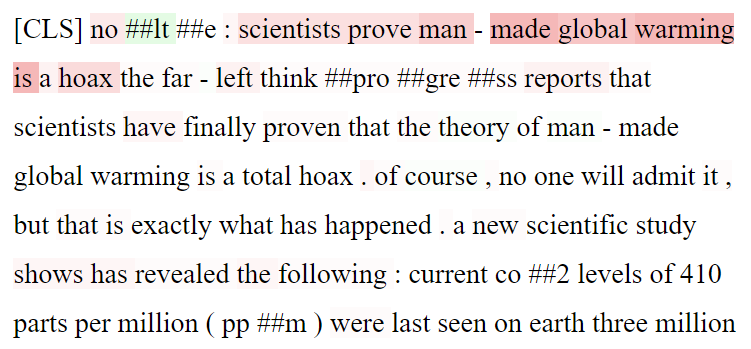
\includegraphics[width=\linewidth]{obrazky-figures/global_warming2.png}
      \caption{BERT model, correctly classified.}
      \label{fig:inter_anal1_a}
    \end{subfigure}%
    \begin{subfigure}{.5\textwidth}
      \centering
      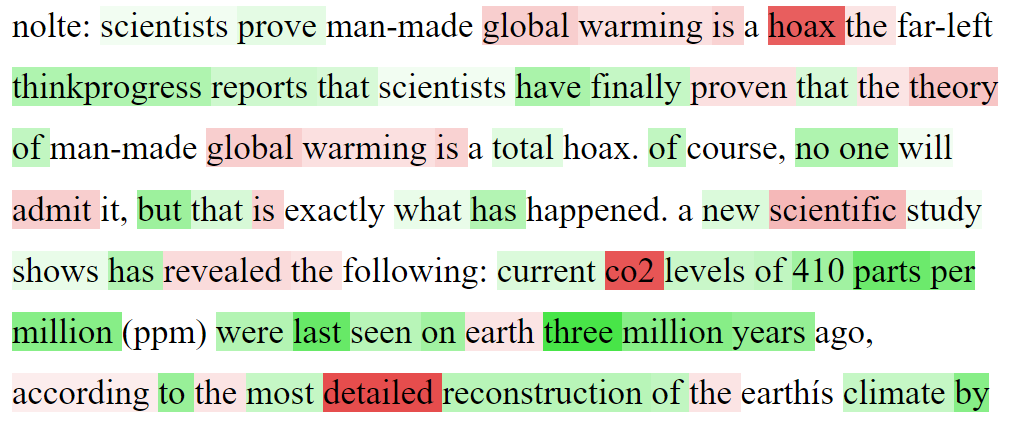
\includegraphics[width=\linewidth]{obrazky-figures/bayes_glob_warm.png}
      \caption{Baseline model, correctly classified.}
      \label{fig:inter_anal1_b}
    \end{subfigure}
    \caption{Visualization of interpretability for an unreliable article with a climate topic.}
    \label{fig:inter_anal1}
\end{figure}

Both models successfully classified the article claiming that global warming is a hoax as unreliable. A potential concern from this observation may be that the models would consider all articles about global warming as unreliable. To test this hypothesis figure \ref{fig:inter_anal2} shows the interpretation of a reliable article about global warming. The baseline model indeed classified the article as unreliable. The BERT model, on the other hand, correctly classified the article and identified \texttt{unesco} as a reliable entity.

\begin{figure}[H]
    \centering
    \begin{subfigure}{.5\textwidth}
      \centering
      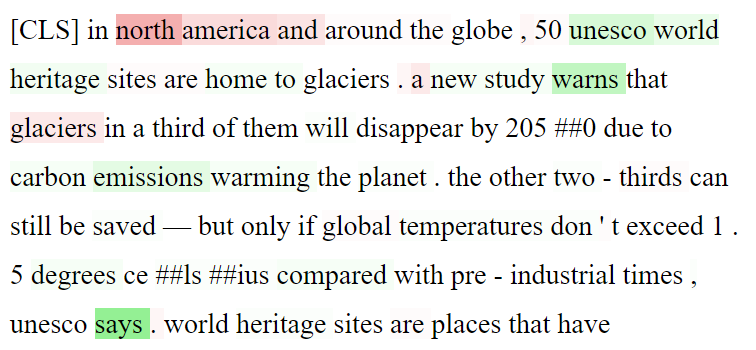
\includegraphics[width=\linewidth]{obrazky-figures/unesco_bert.png}
      \caption{BERT model, correctly classified.}
      \label{fig:inter_anal2_a}
    \end{subfigure}%
    \begin{subfigure}{.5\textwidth}
      \centering
      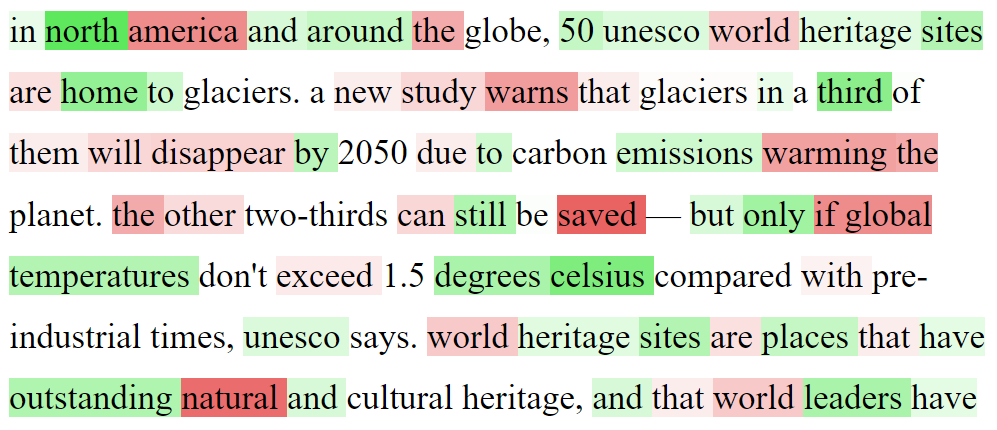
\includegraphics[width=\linewidth]{obrazky-figures/bayes_unecso.png}
      \caption{Baseline model, incorrectly classified.}
      \label{fig:inter_anal2_b}
    \end{subfigure}
    \caption{Interpretability of a reliable article with topic climate.}
    \label{fig:inter_anal2}
\end{figure}

As already noted in chapter \ref{experiments}, the baseline model considers all articles about football as reliable. Figure \ref{fig:inter_anal3} shows the visualization of interpretability for a reliable article about football. Both models correctly classified this article and identified football-related terms like \texttt{arsenal}, \texttt{title}, \texttt{scores}, and \texttt{match} as reliable. The baseline was influenced by the names of players and coaches --- e.g., \texttt{erling haaland}, \texttt{bruyne}, \texttt{pep} --- a lot more than the BERT model.

\begin{figure}[H]
    \centering
    \begin{subfigure}{.5\textwidth}
      \centering
      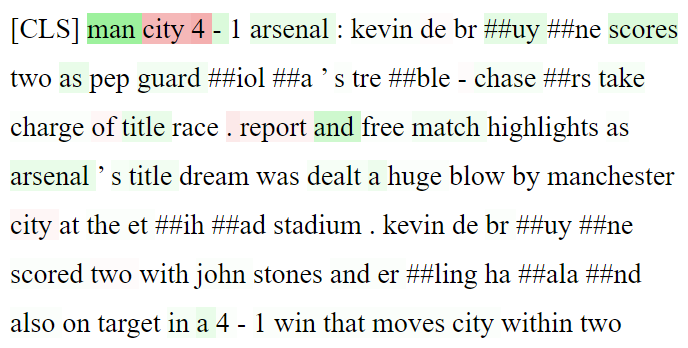
\includegraphics[width=\linewidth]{obrazky-figures/man-city.png}
      \caption{BERT model, correctly classified.}
      \label{fig:inter_anal3_a}
    \end{subfigure}%
    \begin{subfigure}{.5\textwidth}
      \centering
      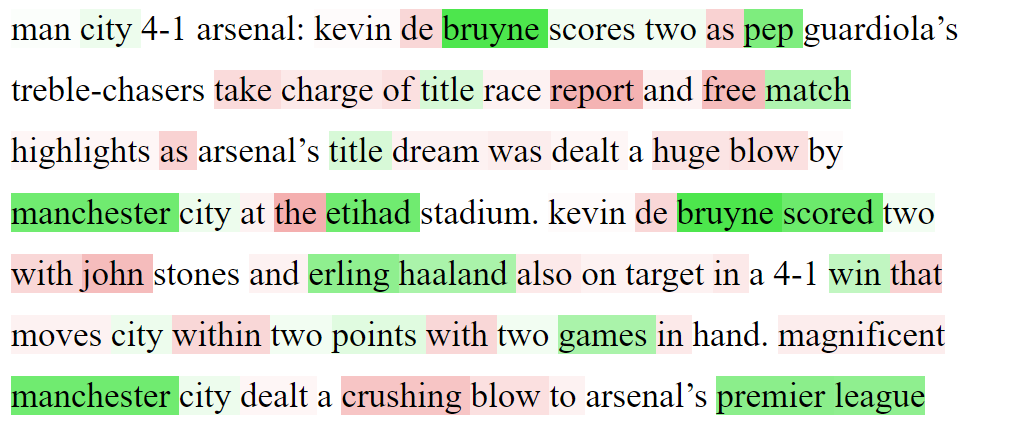
\includegraphics[width=\linewidth]{obrazky-figures/bayes_football1.png}
      \caption{Baseline model, correctly classified.}
      \label{fig:inter_anal3_b}
    \end{subfigure}
    \caption{Interpretability of a reliable article about football.}
    \label{fig:inter_anal3}
\end{figure}

Figure \ref{fig:inter_anal4} shows the interpretability of an unreliable article about football. This article is a fictional story about a reckless football player generated by ChatGPT. The BERT classifier managed to correctly identify it as unreliable as it uses a style similar to tabloid journalism that tries to shock readers through scandals and sensationalism. The baseline also identified the sensationalism in the article but still identified it as reliable because it contains the word \texttt{football}.

\begin{figure}[H]
    \centering
    \begin{subfigure}{.5\textwidth}
      \centering
      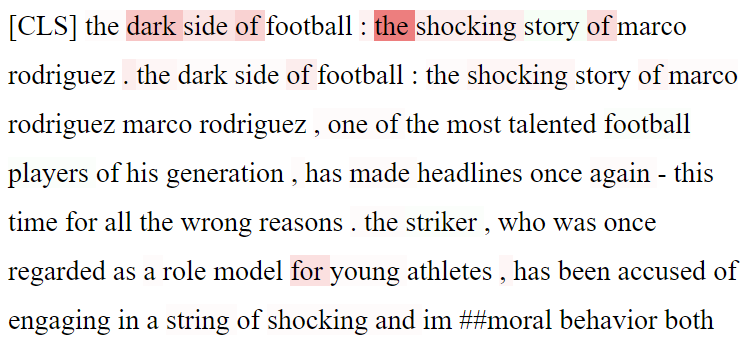
\includegraphics[width=\linewidth]{obrazky-figures/football_fake.png}
      \caption{BERT model, correctly classified.}
      \label{fig:inter_anal4_a}
    \end{subfigure}%
    \begin{subfigure}{.5\textwidth}
      \centering
      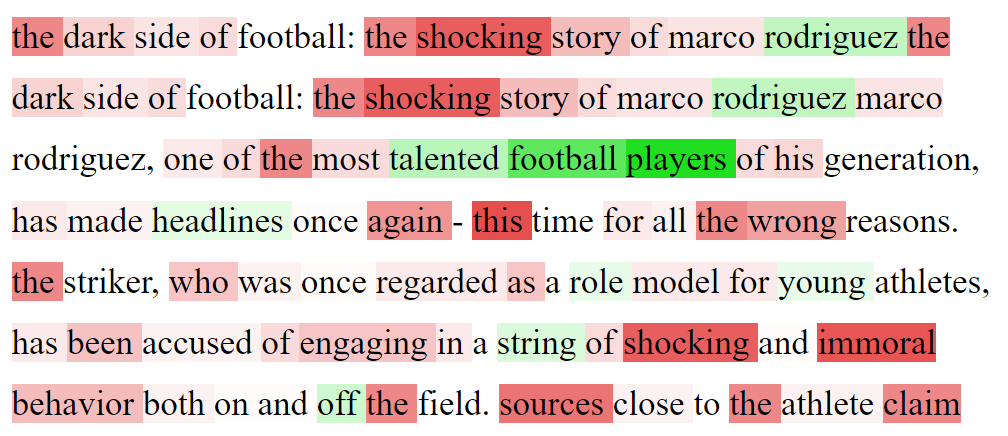
\includegraphics[width=\linewidth]{obrazky-figures/bayes_football2.png}
      \caption{Baseline model, incorrectly classified.}
      \label{fig:inter_anal4_b}
    \end{subfigure}
    \caption{Interpretability of an unreliable article about football generated by ChatGPT.}
    \label{fig:inter_anal4}
\end{figure}
 
Another hypothesis found in chapter \ref{experiments} is that the baseline is not able to correctly classify reliable scientific articles. Figure \ref{fig:inter_anal9} shows the interpretability of such an article. The baseline indeed failed to successfully classify this article. Science-based words like \texttt{nutrient}, \texttt{biomass}, \texttt{research}, \texttt{science} all have a negative contribution to the prediction. 

\begin{figure}[H]
    \centering
    \begin{subfigure}{.5\textwidth}
      \centering
      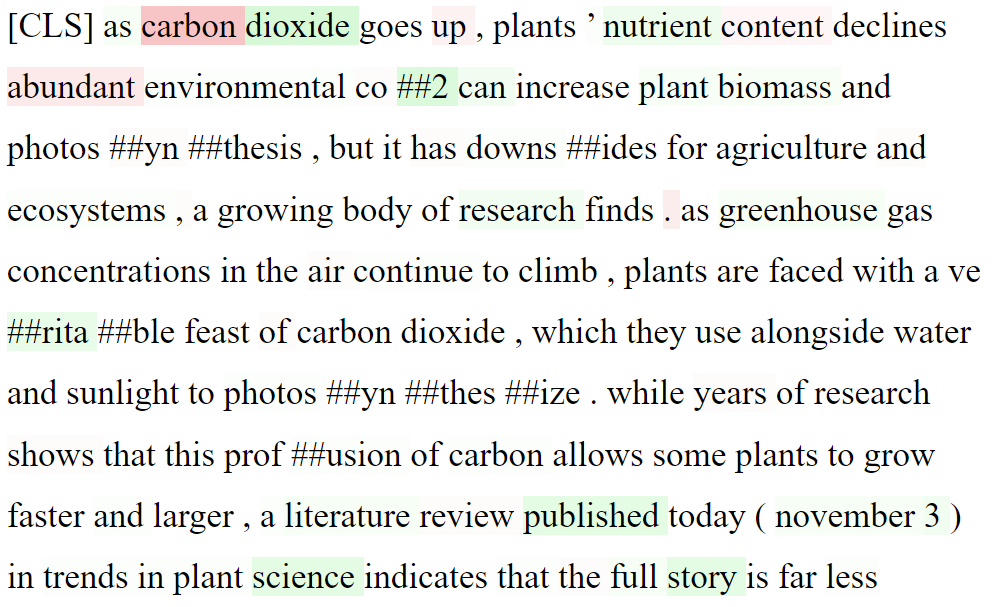
\includegraphics[width=\linewidth]{obrazky-figures/bert_science.png}
      \caption{BERT model, correctly classified.}
      \label{fig:inter_anal9_a}
    \end{subfigure}%
    \begin{subfigure}{.5\textwidth}
      \centering
      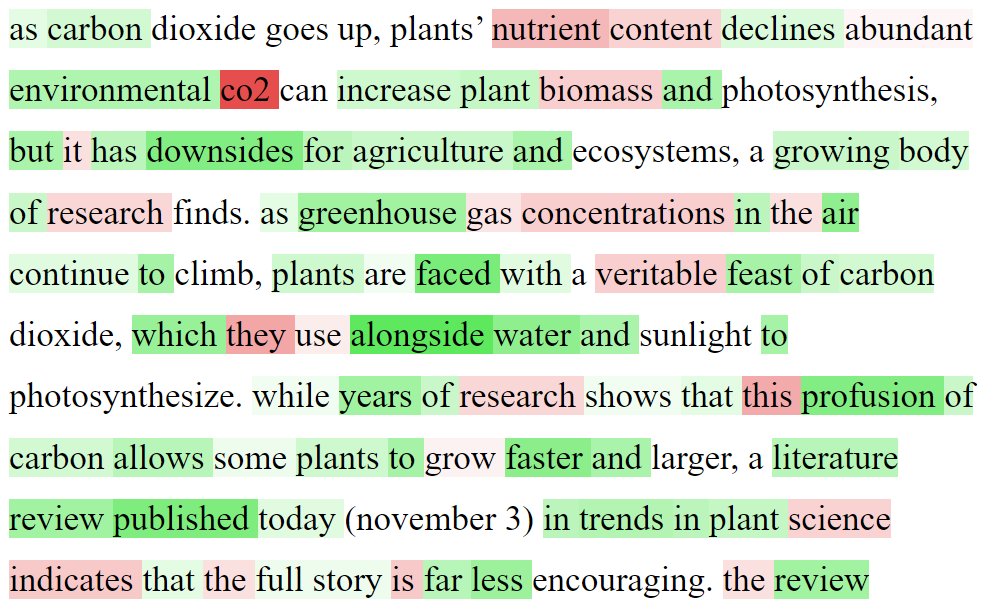
\includegraphics[width=\linewidth]{obrazky-figures/bayes_science.png}
      \caption{Baseline model, incorrectly classified.}
      \label{fig:inter_anal9_b}
    \end{subfigure}
    \caption{Interpretability of a reliable article about science.}
    \label{fig:inter_anal9}
\end{figure}

The BERT model, on the other hand, correctly classified the article as reliable. Figure \ref{fig:inter_anal6} shows a reliable article with the topic of war on which the BERT classifier failed. The cues discovered by the interpretation method seem confusing. On the second row, the word \texttt{reuters} is marked with red and later in the text the same word is green. It is important to note that this may be caused by a different context in each case, however, the interpretation of this article still remains slightly confusing.

\begin{figure}[H]
    \centering
    \begin{subfigure}{.5\textwidth}
      \centering
      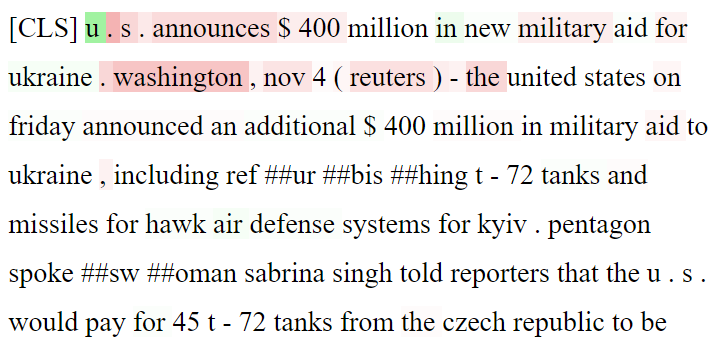
\includegraphics[width=\linewidth]{obrazky-figures/war_fail.png}
      \label{fig:inter_anal6_a}
    \end{subfigure}%
    \begin{subfigure}{.5\textwidth}
      \centering
      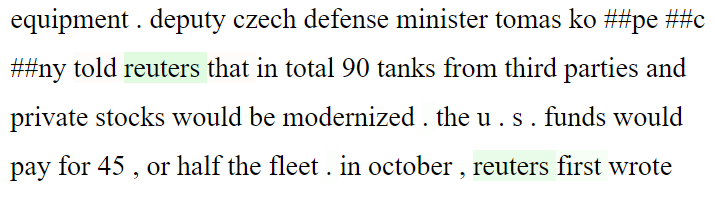
\includegraphics[width=\linewidth]{obrazky-figures/war_fail_reuters.png}
      \label{fig:inter_anal6_b}
    \end{subfigure}
    \caption{Example of a reliable article with the topic of war incorrectly classified by the BERT model as unreliable.}
    \label{fig:inter_anal6}
\end{figure}

Besides using the articles from the FNI dataset, the interpretability was also analysed using one source from the NELA dataset the \texttt{truth theory}. As described in table \ref{tab:bert_acc_per_src} in section \ref{sec:accuracy_per_source}, this reliable source obtained the lowest accuracy of only 19\% from the BERT model. Figure \ref{fig:truth_disc1} shows the interpretability of two articles by this source. 


\begin{figure}[H]
    \centering
    \begin{subfigure}{.5\textwidth}
      \centering
      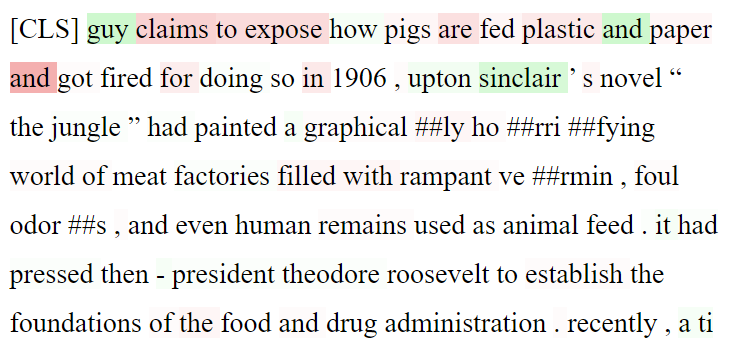
\includegraphics[width=\linewidth]{obrazky-figures/truth-theory1.png}
      \caption{BERT model}
      \label{fig:truth_disc_1a}
    \end{subfigure}%
    \begin{subfigure}{.5\textwidth}
      \centering
      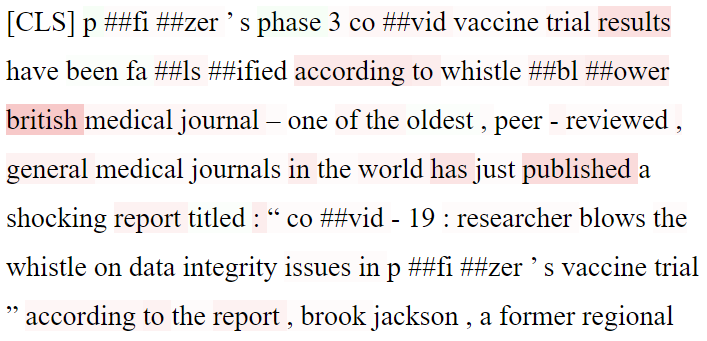
\includegraphics[width=\linewidth]{obrazky-figures/truth-theory3.png}
      \caption{BERT model}
      \label{fig:truth_disc_1b}
    \end{subfigure}
    \caption{Reliable articles by source \texttt{truth theory} classified as unreliable.}
    \label{fig:truth_disc1}
\end{figure}

The \texttt{truth theory} is a source marked as reliable on the MBFC webpage with a high factuality score. After analysing its articles, however, it seemed that the articles are written in a way that resembles fake news and tabloid journalism. Using phrases like \texttt{guy claims to expose how pigs are fed plastic} or \texttt{covid vaccine trial results falsified} really resembles unreliable sources. This source is therefore considered to be an edge case as all the other sources achieved much better accuracy. However, there are also some articles by this source that seem to be reliable and were incorrectly classified. One of these examples is shown in figure \ref{fig:truth_disc2}. In this case, the interpretability is also rather confusing.

\begin{figure}[H]
    \centering
    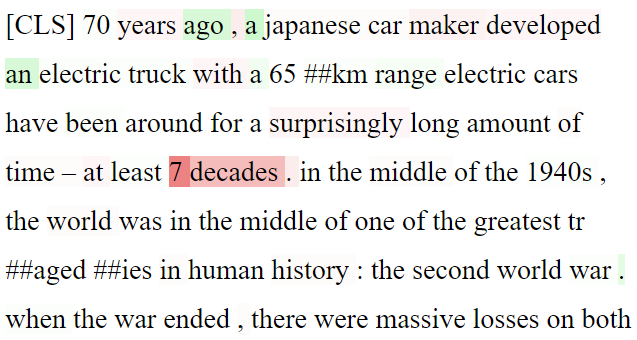
\includegraphics[scale=0.6]{obrazky-figures/truth-theory4.png}
    \caption{Confusing interpretability of a reliable article by source \texttt{truth theory} incorrectly classified by the BERT model as unreliable.}
    \label{fig:truth_disc2}
\end{figure}

Overall the interpretability methods of both classifiers work better on unreliable articles where they are able to identify sensational and shocking headlines. Naturally, it is easier to show that an article is fake rather than prove that it is true. In many reliable articles, the interpretability was not self-explanatory even though the article was correctly classified. A manual analysis of 30 articles showed that the interpretability method of the BERT classifier worked well for 80\% of unreliable and 47\% of reliable articles.



\chapter{Predicting the Credibility of Sources}
\label{chap:source_credibility}
The classifiers implemented in this thesis are constructed to predict the credibility of articles. The goal of this chapter is to find out whether it is possible to use the predicted credibility of articles obtained from the BERT classifier to predict the credibility of media sources. To evaluate the credibility of sources, two different methods were implemented. The first method uses the average credibility of articles published by the given source. The second method creates embeddings from the predicted credibilities of articles and uses them to train a logistic regression model that learns to predict the credibility of sources.
To evaluate these two approaches, the results are compared with ground truth labels and with a state-of-the-art method which uses graph-neighbourhood exploitation algorithms. Following is the explanation of these methods.


\section{Graph-neighborhood Exploitation Method}
The credibility of sources used as the reference for the other two methods was obtained from a method based on graph-neighbourhood exploitation. This method was implemented by Sergio Burdisso (sergio.burdisso@idiap.ch) who kindly shared his results for the purpose of this thesis. As of now, the method has not been officially published and is therefore described only briefly. The method uses citations and references to other sources mentioned in articles to construct a graph, where the nodes represent the sources and the edges represent their relationship based on the citations. Based on this graph it uses reinforcement learning techniques to identify reliable and unreliable sources and compute their credibility. 

The author used 4497 sources crawled from the MBFC website and annotated their reliability following the policy described in the NELA-GT-2019 paper. Each source is assigned a value from $[-1, 1]$ that represents its credibility. These values were transformed to range $[0,1]$ to match the probabilities used by the BERT classifier. Out of the 4497 sources, only 88 were present in the dataset used in this thesis (57 reliable, 31 unreliable). Therefore, these 88 common sources are used to compare the computed credibilities. The following sections describe the methods implemented in this thesis.


\pagebreak

\section{Average Credibility Method}
The first method computes the credibility of a source simply as the average reliability of all articles published by the given source. The articles of the source are all evaluated by the BERT classifier. For each article, the classifier outputs the probabilities of two classes (\texttt{reliable} and \texttt{unreliable}). The probability of the \texttt{reliable} class is used to compute the average. Therefore, the reliability of a source is computed as the average reliability of its articles, predicted by the BERT classifier. Figure \ref{fig:avg_rel} shows a graphical representation of this method.

\begin{figure}[H]
    \centering
    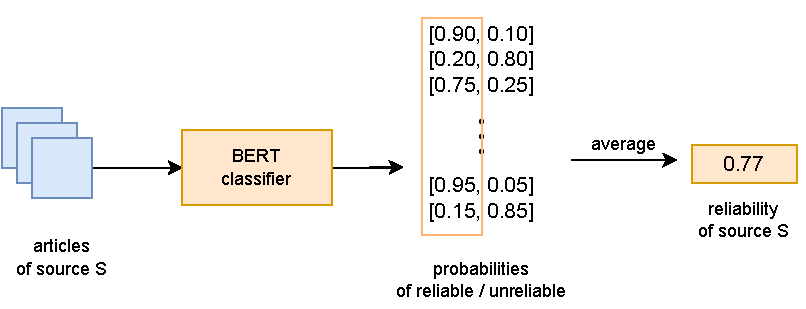
\includegraphics[scale=0.9]{obrazky-figures/avg_reliability.pdf}
    \caption{Computing the reliability of source $S$ using the average reliability method.}
    \label{fig:avg_rel}
\end{figure}


\section{Embedding Method}
The second method uses the probabilities of class \texttt{reliable} predicted by the BERT classifier to create embeddings. All articles are first evaluated by the BERT classifier and the output probabilities of class \texttt{reliable} are sorted in descending order. Then $k$ highest and $k$ lowest values of the predicted reliability are concatenated to create a $2k$-dimensional embedding vector. This vector is then used to train a logistic regression model, which consists of one linear layer with a sigmoid activation function, to predict the reliability of the source based on its embedding. Figure \ref{fig:embeddings} shows the construction of the embedding for source $S$. 

\begin{figure}[H]
    \centering
    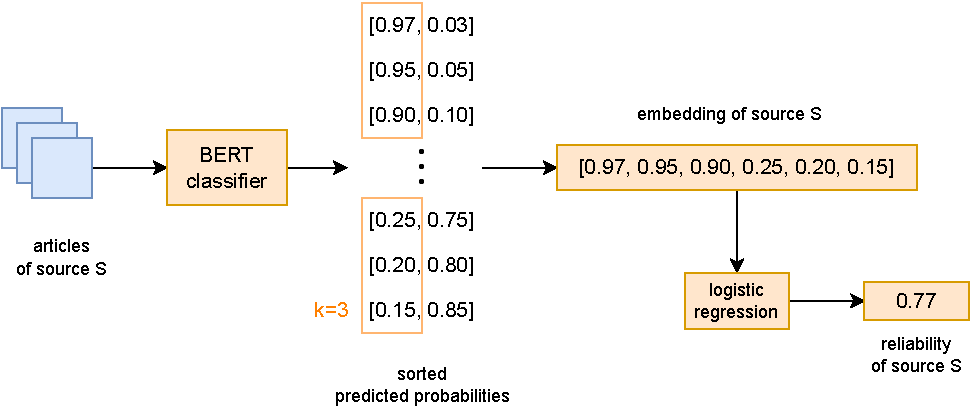
\includegraphics[scale=0.9]{obrazky-figures/embedding.pdf}
    \caption{Computing the reliability of source $S$ using the embedding method with logistic regression for $k=3$.}
    \label{fig:embeddings}
\end{figure}

The embedding vectors often contained very small numbers (e.g., 1.1166e-04, 1.7239e-05, etc.) among the $k$ lowest reliabilities. These numbers are interpreted as zeros by the logistic regression model which made the learning difficult. Normalizing the vector with the L2 norm did not show any improvement nor did applying mean removal. The problem was finally solved by scaling all values of the vector by 10,000. Different values of $k$ were tried and evaluated by comparing the resulting reliabilities of sources with the referential values. The following section discusses the results in detail.

% \begin{figure}[H]
%     \centering
%     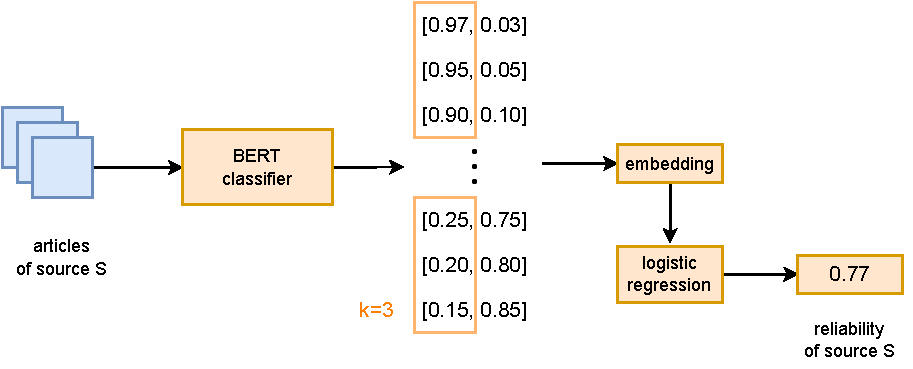
\includegraphics[scale=0.9]{obrazky-figures/emb_log_reg.pdf}
%     \caption{Computing the reliability of sources using the logistic regression method with embeddings.}
%     \label{fig:log_reg}
% \end{figure}

\section{Comparing the Results}
The implemented methods are evaluated by comparing their results with ground truth labels and the referential scores obtained from the graph-neighbourhood method. Both methods were trained on the articles from the NELA test set. The test set contains 249 sources and 88 of them are also present in the referential scores. Therefore these 88 sources were only used for evaluation, not for training of the average reliability and embedding methods. To compare the computed reliabilities with the referential scores the Jensen-Shannon distance and Kendall rank methods are used. 

\subsection*{Jensen–Shannon Divergence}
The Jensen–Shannon (JS) divergence, presented in \cite{js_divergence}, is based on the Kullback-Leibler (KL) divergence. The KL divergence score quantifies how much one probability distribution differs from another probability distribution. The KL divergence between two distributions $P$ and $Q$ is computed using the following equation.

\begin{equation}
    KL(P || Q) = \sum_{x \in X} P(x) \cdot \operatorname{log}\frac{P(x)}{Q(x)}
    \label{eq:kl_divergence}
\end{equation}

where $P(x)$ and $Q(x)$ are the probabilities of $x$ in distributions $P$ and $Q$. The KL divergence is not symmetric as $KL(P||Q) \neq KL(Q||P)$. The Jensen-Shannon (JS) divergence uses the KL divergence to calculate a normalized score that is symmetrical. The computation of JS divergence is described by equation \ref{eq:js_divergence}. 

\begin{equation}
    JS(P||Q) = \frac{1}{2} \cdot KL(P||M) + \frac{1}{2} \cdot KL(Q||M) 
    \label{eq:js_divergence}
\end{equation}

where $M = \frac{1}{2} (P+Q)$. The JS divergence computes symmetrical values --- meaning $JS(P||Q) = JS(Q||P)$ --- ranging from 0 (distributions $P$ and $Q$ are identical) to 1 (biggest difference) when using the base-2 logarithm. Finally, the JS distance used in this thesis is simply the square root of the JS divergence.

\begin{equation}
    JS_{distance}(P||Q) = \sqrt{JS(P||Q)}
    \label{eq:js_distance}
\end{equation}

\subsection*{Kendall Rank Correlation Coefficient (Tau)}
The second metric used for comparing the results is the Kendall rank correlation coefficient, also known as the Kendall tau. This method is used when the compared variables are ordinal or ranked data. It measures the strength of the association between two variables and the direction of the relationship. The computation of Kendall tau is based on the appearance of concordant and discordant pairs in the data. Imagine we compare two columns of ranked data $X$ and $Y$. A pair of observations $(x_i, y_i)$ and $(x_j, y_j)$ where $i < j$ are concordant when the following statement is true:

$$(x_i > x_j) \wedge (y_i > y_j) \quad \lor \quad (x_i < x_j) \wedge (y_i < y_j)$$

otherwise, the pairs of observations are considered discordant. The number of concordant and discordant pairs between $X$ and $Y$ is counted and used to compute the rank. Several versions of the Kendall tau exist. In this thesis, the tau-b version is used as it accounts for ties in the columns. The Kendall tau-b uses the following equation\footnote{\url{https://docs.scipy.org/doc/scipy-0.15.1/reference/generated/scipy.stats.kendalltau.html}}:

\begin{equation}
    \tau_b = \displaystyle{\frac{P - Q}{\sqrt{((P+Q+T) \cdot (P+Q+U))}}}
\end{equation}

where $P$ is the number of concordant pairs, $Q$ is the number of discordant pairs, $T$ is the number of ties in $X$ and $U$ is the number of ties in $Y$. If a tie occurs for the same pair in both $X$ and $Y$, it is not added to either $T$ or $U$. The value of Kendall tau ranges from -1 to 1. The closer to 0 the lower the association between $X$ and $Y$. The further from 0 the bigger is the association. The negative sign only indicates the direction of the relationship. 

Table \ref{tab:js_kt_resluts} shows the results of JS distance and Kendall tau of the two methods (using the BERT classifier and average reliability/embeddings) compared with the referential reliability scores of sources obtained from the graph-neighbourhood method. Both methods obtained values around 0.2 for the JS distance (where 0 indicates identical distributions and 1 indicates the biggest difference). The embedding method outperformed the average reliability in both metrics, however for different values of $k$. It achieved the best tau value of 0.63 for $k=22$ and the best JS distance for $k=4$.

\begin{table}[H]
    \centering
\begin{tabular}{|c|c|c|}
\hline
\textbf{Method} & \textbf{JS distance} & \textbf{Kendall tau} \\ \hline
avg reliability & 0.21                 & 0.51                 \\ \hline
embeddings (k=4)      & 0.20                 & 0.56                 \\ \hline
embeddings (k=22)     & 0.25                 & 0.63                 \\ \hline
\end{tabular}
    \caption{Results of JS distance and Kendall tau of the average reliability and embedding methods compared with the referential values.}
    \label{tab:js_kt_resluts}
\end{table}

Figure \ref{fig:tau_js_vs_k} shows the Kendall tau and JS distance of the embedding method for different values of $k$ from 1 to 30. The value of $k$ represents how many article reliability scores are used to create the embedding. It also influences the required number of articles for each source, e.g., when $k=10$ all sources must contain at least 20 articles to create the embedding. In cases where the source contains fewer articles than is required, the embedding uses zeros as padding at the end. A growing tendency can be seen in figure \ref{fig:tau_vs_k}, indicating that the logistic regression method improved with longer embeddings. It is interesting to see that with the growing value of $k$ the tau value is improving whereas the JS distance deteriorates. The change in JS distance, however, is not as significant as all values are between 0.2 and 0.26. On the other hand, the tau value managed to improve from 0.45 to 0.63. Therefore it seems that a bigger number of embeddings improves the ordering of the computed reliability, but the accuracy of the scores remains approximately the same. 

\begin{figure}[H]
    \centering
    \begin{subfigure}{.5\textwidth}
      \centering
      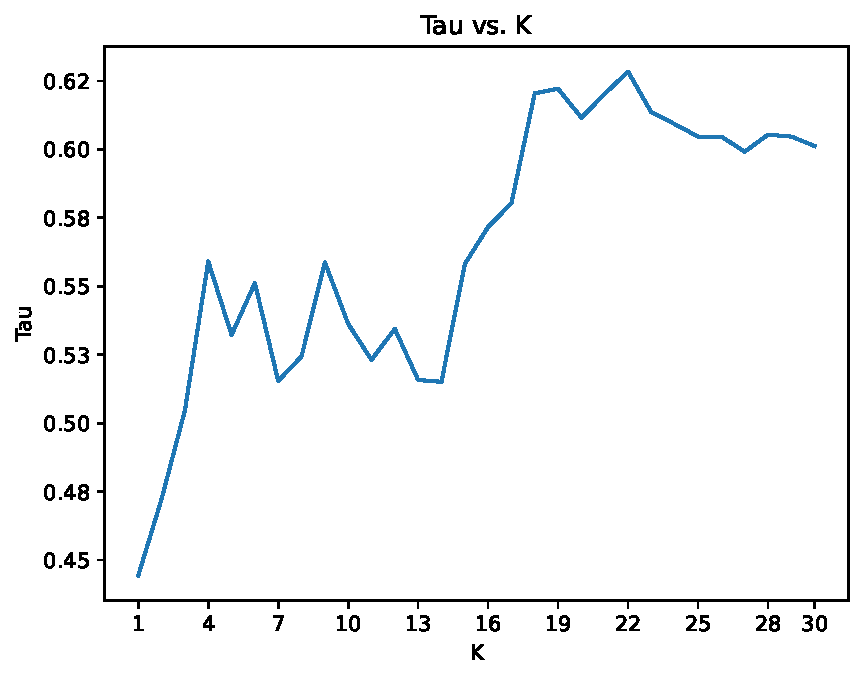
\includegraphics[width=\linewidth]{obrazky-figures/tau_vs_k30.pdf}
      \caption{}
      \label{fig:tau_vs_k}
    \end{subfigure}%
    \begin{subfigure}{.5\textwidth}
      \centering
      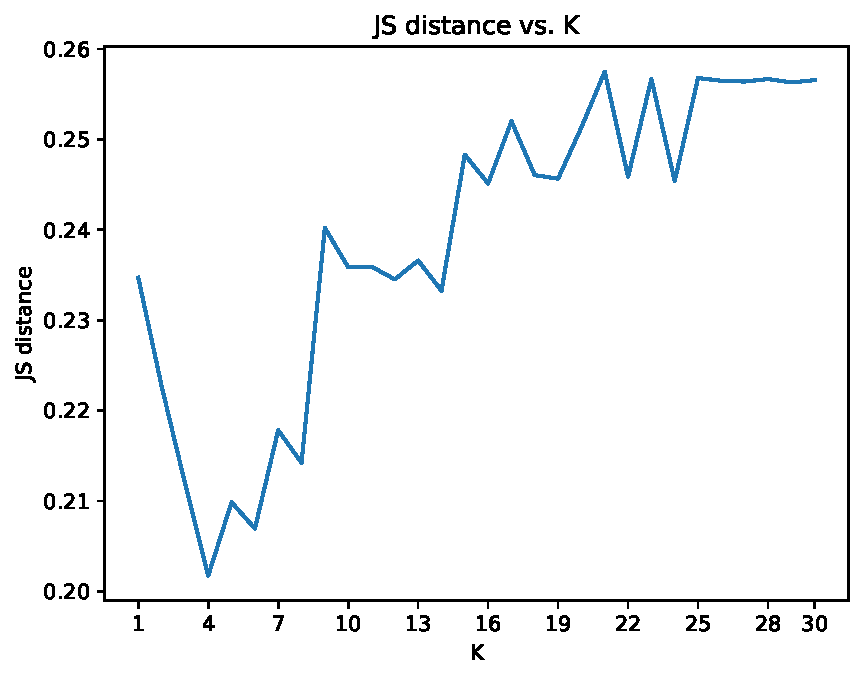
\includegraphics[width=\linewidth]{obrazky-figures/js_vs_k30.pdf}
      \caption{}
      \label{fig:js_vs_k}
    \end{subfigure}
    \caption{Kendall tau and JS distance of the embedding method based on the value of $k$.}
    \label{fig:tau_js_vs_k}
\end{figure}

To see how the values of tau and JS vary, they were computed separately for four groups of sources. Each group is chosen randomly and contains around 20 sources. The results for the embedding method with $k=22$ are displayed in figure \ref{fig:tau_vs_k_groups}.

\begin{figure}[H]
    \centering
    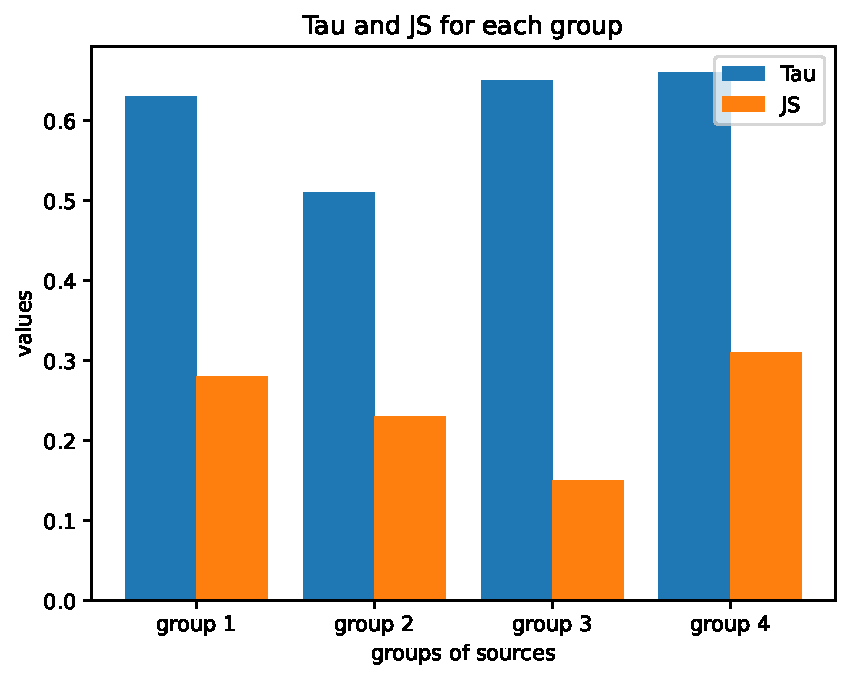
\includegraphics[scale=0.6]{obrazky-figures/tau_js_groups.pdf}
    \caption{Kendall tau and JS distance of the embedding method with $k=22$ for different groups of approximately 20 sources.}
    \label{fig:tau_vs_k_groups}
\end{figure}

Besides comparing the computed source reliabilities with the referential scores they were also compared with the ground truth labels. Figure \ref{fig:accuracy_vs_threshold} shows the accuracy of both methods for different values of threshold. The threshold is used to determine the label of a source based on the computed reliability score. If the score is higher than the selected threshold the source is considered reliable, otherwise it is considered as unreliable. An interesting observation is that the accuracy is above 90\% for most of the threshold values. This is explained when looking at the average predicted score for each label. Unreliable sources have an average predicted score of 0.07 and reliable sources have an average score of 0.93 (for the average probability method). Still, the best threshold value was found to be 0.6 as it performs the best for all approaches.

\begin{figure}[H]
    \centering
    \begin{subfigure}{.5\textwidth}
      \centering
      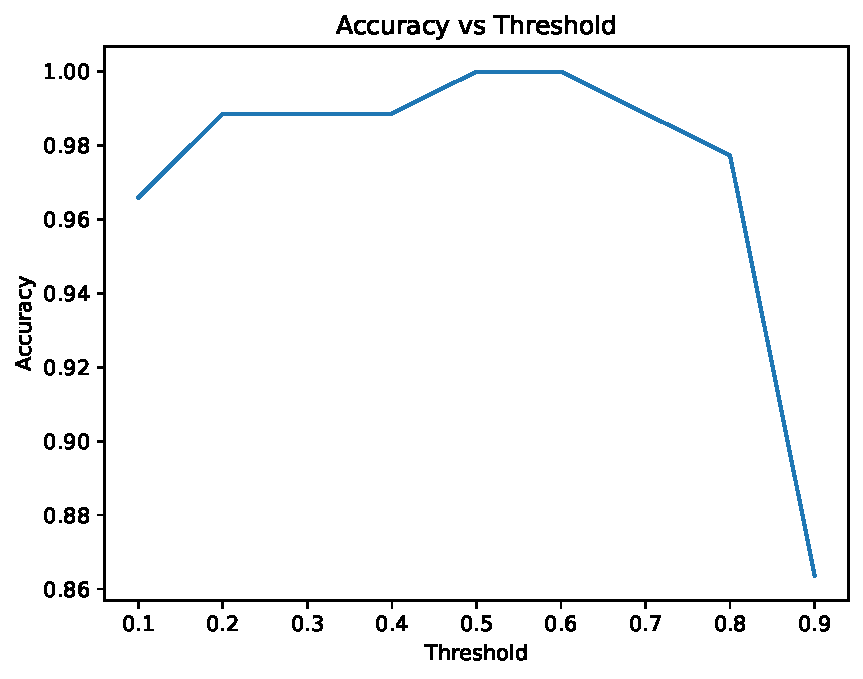
\includegraphics[width=\linewidth]{obrazky-figures/accuracy_vs_threshold_avg.pdf}
      \caption{Average credibility method.}
      \label{fig:accuracy_vs_logreg}
    \end{subfigure}%
    \begin{subfigure}{.5\textwidth}
      \centering
      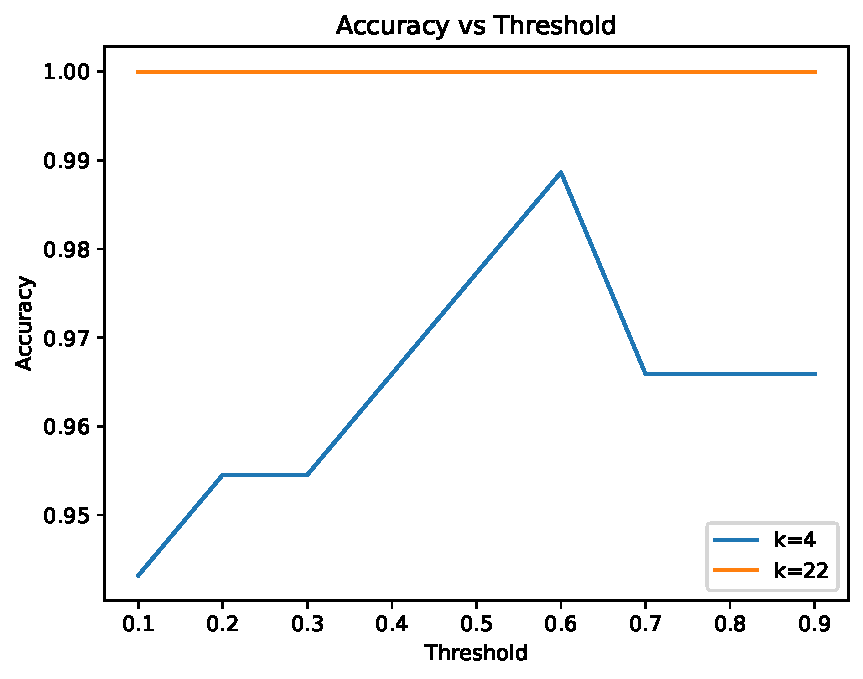
\includegraphics[width=\linewidth]{obrazky-figures/accuracy_vs_threshold_logreg.pdf}
      \caption{Embedding method.}
      \label{fig:accuracy_vs_avg}
    \end{subfigure}
    \caption{Accuracy of the embedding and average credibility methods for different thresholds.}
    \label{fig:accuracy_vs_threshold}
\end{figure}


The conclusion of this experiment is therefore that a classifier computing reliability scores of articles based only on text can be used to assess the reliability of media sources on the internet.



%%%%%%%%%%%%%%%%%%%%%%%%%%%%%%%%%%
% Conclusion
\chapter{Conclusion}
\label{conclusion}
The goal of this thesis was to study the biases and cues exploited by content-based methods in the text of fake news articles and evaluate their performance on predicting the reliability of articles and media sources. The first step was to define the problem of fake news detection and study the methods and previous work in this area. After that, a comprehensive analysis of available datasets was conducted. Each dataset was evaluated for its qualities and suitability for this thesis.

The most suitable dataset was found to be the NELA-GT-2021 dataset and was therefore used to train the classifiers in this thesis. This dataset was preprocessed by extending the source-level labels (indicating the reliability of sources) to article-level labels as each article obtained the label of its source. Another preprocessing step was filtering keywords from the dataset (e.g., names of sources and specific terms) that would provide simple clues for the classifiers making them base the predictions on simple clues rather than actually understanding the text.
Another two datasets were created for testing and analysis. The first one called the Merged dataset, was formed by merging three fake news datasets with article-level labels and was used for further evaluation of the classifiers. The second dataset called the Fake News Interpretability (FNI) dataset, was created by the author of this thesis. It consists of 46 manually collected articles (23 reliable and 23 unreliable) from various sources on the internet. Each article is assigned a topic that reflects what is its content related to. The topics of the articles were used to analyse the performance of the classifiers in different areas.

For the implementation of the classifiers, two different methods were selected. The first method implements the baseline model and is based on TF-IDF and a Multinomial Naive Bayes classifier. The second method intended to improve the baseline uses the BERT transformer. 
Both classifiers were evaluated on a test split of the NELA dataset, the Merged dataset and the FNI dataset. The analysis revealed several strengths and weaknesses of both classifiers. The baseline was not very successful in classifying reliable articles. It achieved a very low accuracy of only 48\% on articles with a pro-science bias (science-based articles using credible scientific sourcing) as well as on articles with a very high factuality score (62\% accuracy). The average accuracy per source for unreliable articles was 83\% whereas for reliable articles only 71\%. The baseline was also not able to identify unreliable articles about football as it learned to connect football-related terms with a sign of reliability.
The BERT classifier managed to outperform the baseline in every aspect and mitigated its disabilities. The difference between the average accuracy per source for unreliable and reliable articles was not so significant (only 3\%). The BERT classifier performed much better in classifying the pro-science articles (94\% accuracy) and articles with a very-high factuality (97\% accuracy). The BERT classifier also managed to identify fake articles about football, a topic considered reliable by the baseline. Among the limitations of the implemented classifiers can be the fact that both methods can be used only for text and cannot be applied to other types of media (e.g., video, images, etc.).

For the BERT classifier, a method of interpretability based on Integrated gradients was implemented. The interpretability was analysed using articles from the FNI dataset and one reliable source from the NELA dataset that achieved the lowest accuracy. This reliable source with a high factuality score achieved an accuracy of only 19\%. After analysing its articles it seemed like the source often uses shocking headlines and style-of-writing similar to unreliable articles. The interpretability method worked better for unreliable articles and was able to identify the shocking headlines they often use. For reliable articles, the results were often inconsistent. A manual analysis of 30 articles showed that the Integrated gradients method worked well for 80\% of unreliable and 47\% of reliable articles.

The implemented classifiers were also evaluated for their ability to predict the reliability of sources using the computed reliability of their articles. Two methods were created and their results were compared with referential values obtained from a state-of-the-art method using graph exploitation. The results showed that a classifier constructed to compute the reliability of articles can be successfully applied to media sources. 

This thesis succeeded in creating a functional classifier for predicting the credibility of articles and sources on the internet using only the text of articles. The method of interpretability performed well in identifying the sensationalism used in fake articles but showed uncertainty in identifying reliability. A more complex method could be applied in future work, e.g., a masker neural network inspired by the masker model in \cite{claim-dissector} —-- a model that learns to mask the least number of tokens to change the decision of the classifier, where the tokens that were masked represent the most important tokens for the decision. The content-based classifier created in this thesis could further be applied to downstream tasks, e.g., to improve an existing fact-checking model by assigning reliability to the documents used as evidence.
  \else
    % Tento soubor nahraďte vlastním souborem s obsahem práce.
%=========================================================================
% Autoři: Michal Bidlo, Bohuslav Křena, Jaroslav Dytrych, Petr Veigend a Adam Herout 2019
\chapter{Úvod}

Tento text slouží jako ukázkový obsah šablony a současně rekapituluje nejdůležitější informace z předpisů a poskytuje další užitečné informace, které budete potřebovat pro tvorbu technické zprávy ke svojí práci. Než se šablonou budete dále pracovat, je třeba vědět, jak ji správně použít. To je stručně uvedeno v~příloze \ref{jak}.

I když některým studentům pro napsání dobré diplomové práce (bakalářská práce je také diplomová -- dostává se za ni diplom) stačí znát a dodržovat oficiální formální požadavky uvedené ve směrnicích a typografické zásady, často je výhodné před započetím psaní zjistit, jaké jsou osvědčené postupy pro psaní odborného textu a jak si práci usnadnit. Někteří vedoucí svým studentům připravili popisy osvědčených postupů, které vedly k desítkám úspěšně obhájených prací. Výběr nejzajímavějších postupů, které měli autoři této šablony k~dispozici ve chvíli její tvorby, je v níže uvedených kapitolách. Má-li Váš vedoucí svoji stránku s doporučenými postupy, tyto kapitoly můžete vynechat a řídit se pokyny svého vedoucího. Pokud takovou stránku nemá, může být přečtení níže uvedeného textu vhodnou přípravou na konzultaci o plánované struktuře a náplni textu práce.

Diplomová práce je rozsáhlé dílo a tomu odpovídá i technická zpráva. Ne každý je schopen si sednout a jednoduše ji napsat. Je třeba vědět, kde začít a jak postupovat. Jedním z možných přístupů je začít psaním klíčových slov a abstraktu, abyste si ujasnili, co je v~práci nejdůležitější. O tom pojednává kapitola \ref{abstrakt}.

Po sepsání abstraktu se lze pustit do psaní samotného textu technické zprávy. Typicky si nejprve připravíme základní strukturu práce, kterou pak budeme plnit textem. Kapitola \ref{struktura} se zabývá základními informacemi a radami pro psaní odborného textu, které Vám pomohou vyhnout se začátečnickým chybám, a stanovením nadpisů kapitol a přibližných rozsahů jednotlivých částí práce. V závěru kapitoly je pak uveden přístup, kterým si lze psaní technické zprávy značně usnadnit.

Diplomové práce v oblasti informačních technologií mají určitou typickou strukturu. Po~úvodu bude následovat kapitola či kapitoly zabývající se shrnutím současného stavu, který bude v následujících kapitolách zhodnocen a bude navrženo řešení, které bude implementováno a otestováno. V závěru pak budou výsledky vyhodnoceny a bude navržen budoucí vývoj. I když se názvy a rozsahy kapitol v různých pracích liší, vždy tam lze najít kapitoly odpovídající této struktuře. Kapitola \ref{kapitoly} se zabývá obsahy typických kapitol, které se v diplomových pracích z oblasti IT vyskytují. Většina studentů ve svojí práci pravděpodobně využije pouze určitou podmnožinu popsaných kapitol, která je pro jejich práci relevantní. Uvedené popisy a rady mohou pomoci jak s~rozhodnutím, zda danou kapitolu uvést, tak i~s~vnitřní strukturou a samotným obsahem kapitoly.

Za závěrečnou kapitolou práce vždy následuje seznam použité literatury. Citacemi, které tento seznam tvoří, a odkazy na ně se zabývá kapitola \ref{citace}. Byť to tak nezkušený student nemusí vnímat, je seznam použité literatury a odkazy na něj pro práci zcela zásadní. Hodnocení práce s literaturou a citací tvoří jednu z důležitých částí posudku oponenta a bude-li chybět jediná položka, může to vést k hodnocení stupněm F, následnému disciplinárnímu řízení za plagiátorství a k vyloučení z nedokončeného studia. Nesprávná práce se zdroji může mít i další důsledky -- v roce 2018 stála křesla dva členy české vlády. Proto prosím citacím věnujte odpovídající pozornost. 

Po dokončení textu je nutné zjistit, jaké požadavky jsou kladeny na vysokoškolskou kvalifikační práci na FIT VUT v~Brně, a dořešit případné nedostatky. Formální požadavky jsou uvedeny ve směrnicích a na webových stránkách, které jsou zmíněny v kapitole \ref{formality}. Tato kapitola obsahuje i požadované rozsahy jednotlivých typů prací a další vybrané informace z~předpisů a doporučení. V závěru kapitoly je uveden přehled nejčastějších chyb, se kterými se oponenti setkávají a kterým byste se měli vyhnout. Hodnocení formální úpravy práce je pak další z důležitých součástí posudku oponenta.

Po odstranění formálních nedostatků lze práci odevzdat. Před odevzdáním práce si můžete projít kontrolní seznam (tzv. \uv{checklist}) uvedený v příloze \ref{checklist}. Samotné odevzdání listinné i elektronické verze práce je pak popsáno v kapitole \ref{odevzdani}.

V závěrečné kapitole \ref{zaver} je pak uvedeno shrnutí toho, co se lze přečtením tohoto textu dozvědět, a to nejdůležitější, na co je třeba myslet před odevzdáním práce.


\chapter{Abstrakt}
\label{abstrakt}
Pod nadpisem Abstrakt je uvedeno shrnutí práce zabírající prostor maximálně 10 řádků. Z~dobrého abstraktu by mělo být i přes jeho malý rozsah patrné, jaký problém se řešil, jaký přístup k jeho řešení byl v práci použit a jakých výsledků bylo dosaženo. Účelem abstraktu je, aby potenciální čtenář práce již po přečtení abstraktu věděl, zda v práci najde to, co hledá \cite{fitWeb}. Zbytek této kapitoly byl převzat z blogu prof. Herouta \cite{Herout}.
\bigskip

\noindent Za prvé – na abstraktu záleží. Za druhé – není těžké ho napsat. Pojďme na to.

\subsection*{K čemu je abstrakt}
Abstrakt slouží k \bf vyhledávání\rm, společně s názvem dané vědecké práce a seznamem klíčových slov. Tyto části (snad s výjimkou názvu) nejsou přímo součástí textu a nečeká se, že někdo, kdo by zasedl ke čtení dané vědecké práce, bude číst je. To, že práci čte, znamená, že už se dostal za fázi čtení abstraktu. Abstrakt mu slouží ve chvíli, kdy se ještě rozhoduje, \bf zda vůbec \rm text číst.

Když někdo tam venku hledá odpověď na svůj problém, zadá knihovnici nebo dnes spíše vyhledávacímu serveru klíčová slova, která se jeho potíží dotýkají. Na základě shody těchto klíčových slov a klíčových slov uvedených autory dostane seznam názvů prací, které by mu mohly nabízet řešení. Dobře sestavený název práce badateli pomůže vytipovat takové texty, které by mohly mít vztah k jeho problému a mohl by se zajímat o jejich přečtení.

A tady právě přichází na scénu abstrakt. Badatel si čte abstrakt vytipovaných prací a~rozhoduje se, zda práci skutečně chce číst, nebo jestli se v tomto případě jeho filtr založený pouze na jednořádkovém nadpisu zmýlil.

V tuto chvíli obvykle ještě nemá stažené nějaké PDF s celým textem, natož aby měl v ruce vytištěný fascikl. Abstrakty jsou určeny k tomu, aby byly \bf mimo text\rm , aby ležely na serverech agregujících vědecké texty. Proto první pravidlo je, že abstrakt musí fungovat samostatně -- pokud obsahuje odkazy do literatury nebo se odvolává na text (\uv{Výkonnost metody je přehledně shrnuta na straně 51.}), nedělá badateli dobrou službu, což badatel ocení tím, že si o autoru nepomyslí nic hezkého, práci si nepřečte a autora neocituje.

\subsection*{Kdy a jak psát Abstrakt}
Může dávat smysl psát abstrakt na závěr celého psaní -- jako shrnutí a skutečné anotování sepsaného díla. Já jsem vyznavačem opačného přístupu -- abstrakt píšu na samém začátku. Když píšu vědecký článek, začínám sepsáním velkého počtu klíčových slov, jež se textu dotýkají. Bývá jich více, než potom uvedu jako ona charakteristická klíčová slova používaná k indexování. Ujasňuji si tím prostor, kde se článek pohybuje -- o čem je třeba hovořit, co je v textu podstatné, čeho se dotýká. Hned po ujasnění klíčových slov formuluji nadpis a~právě abstrakt. 

Považuji za mimořádně užitečné ujasnit si právě ony čtyři části abstraktu -- Jaký problém se řeší? Jaké řešení práce nabízí? Jaké jsou přesně výsledky? Jaký je jejich význam? Když je toto jasné, text se píše skoro sám. Pokud toto má být nejasné, jak u všech všudy je možné vůbec dát dohromady smysluplnou větu v samém textu?

\subsection*{Doporučená struktura abstraktu}
Abstrakt vědecké práce se může skládat ze čtyř částí a pak být opravdu užitečný. Každá část se bude skládat z nějakých dvou, tří vět, někdy postačí jedna.

V byznysu se vžil slovesný útvar \uv{elevator pitch} -- představení ve výtahu. Ne náhodou jeho struktura připomíná právě doporučovanou strukturu abstraktu. Opravdu, autor odborného textu má do abstraktu napsat právě to, co by říkal o své práci, kdyby na to měl nejvýše dvě minuty a nemohl použít žádných slajdů, obrázků, textu. O čem by tedy měl mluvit?

\paragraph{První část -- Jaký se řeší problém? Jaké je téma? Jaký je cíl textu?}
\begin{itemize}
  \item{Tato práce řeší.}
  \item{Cílem této práce je.}
  \item{Zaměřil jsem se na.}
\end{itemize}
Nepatří sem úvodní pohádky charakteristické pro špatný odborný sloh: \uv{Naše poslední pětiletka staví před nás nové a smělé cíle}, \uv{S rozvojem výpočetní techniky a zejména zobrazovacích zařízení je stále důležitější \ldots} Ty nepatří do dobrého textu nikam, ale do~abstraktu tím méně. Pokud dokážete vyjádřit účel svého textu v jedné větě o pár slovech, udělejte to a nepřidávejte nic navíc. Stručnější zde vždy znamená lepší.

\paragraph{Druhá část -- Jak je problém vyřešen? Cíl naplněn?}
\begin{itemize}
  \item{Zvolený problém jsem vyřešil pomocí toho a toho.}
  \item{V řešení bylo použito metody té, postupu toho a analýzy oné.}
  \item{Práce představuje algoritmus takový, který.}
  \item{Data jsem zpracovával pomocí těch a těchto nástrojů a provedl vyhodnocení takové.}
  \item{Podstatou našeho algoritmu je.}
\end{itemize}

Pokud je podstatou sepisovaného odborného textu nová metodologie (= \uv{jak něco dělat}), patří přesně sem její popis. Pokud se představované řešení skládá ze tří částí, pravděpodobně v této části abstraktu budou tři věty, z nichž každá se bude věnovat jedné části řešení. Dobrý abstrakt v této části bude upřímný a přesný -- nebude si schovávat \uv{odhalování svých tajemství} až do textu. Vágní formulace podstaty řešení v abstraktu obvykle znamená, že autoři buď neumí psát a nebo vlastně nemají o čem -- ani jedno není zrovna výzva ke stažení a čtení mnoha stran textu.

\paragraph{Třetí část -- Jaké jsou konkrétní výsledky? Jak dobře je problém vyřešen?}
\begin{itemize}
  \item{Podařilo se dosáhnout úspěšnosti 87,3\,\%.}
  \item{V práci jsme vytvořili systém, který.}
  \item{Vytvořené řešení poskytuje ty a ty možnosti.}
  \item{Provedeným výzkumem jsme zjistili, že.}
\end{itemize}

Není špatným zvykem uvést v této části konkrétní číslo -- \uv{existující metodu XY jsme zrychlili pětkrát}. Pokud přínos práce není možné shrnout do dvou nebo tří vět, někde je něco velmi špatně a celý text pravděpodobně nestojí za psaní.

\paragraph{Čtvrtá část -- Takže co? Čím je to užitečné vědě a čtenáři?}
\begin{itemize}
  \item{Přínosem této práce je.}
  \item{Hlavním zjištěním je.}
  \item{Hlavním výsledkem je.}
  \item{Na základě zjištěných údajů je možné.}
  \item{Výsledky této práce umožňují.}
\end{itemize}

Při psaní vědeckých článků já sám obvykle bojuji s podobností části třetí a čtvrté. Vskutku, obě hovoří o tom, co jsou výsledky a přínosy textu. Účelem třetí části je jmenovitě a konkrétně jmenovat dosažené výsledky, úkolem části čtvrté je interpretovat jejich význam. Asi ničemu nevadí, když tato dvě sdělení do jisté míry splynou a část třetí a čtvrtá nejen že nemají každá vlastní odstavec, ale prolínají se dokonce ve společných větách.

\paragraph{Nultá část -- O co jde? Kde jsme?}
\begin{itemize}
  \item{Práce je řešena v kontextu tom a tom.}
  \item{Nauka ta a ta se zabývá studiem toho a toho.}
  \item{Stavíme na těchto a oněch nedávných pokrocích v naší oblasti.}
\end{itemize}

Někdy je nutné na sám začátek abstraktu vložit kratičké uvedení kontextu, ve kterém se~celá záležitost vlastně odehrává. Může to být přínosné~u vskutku obskurního a esoterického oboru, který leží stranou hlavního proudu. Obvykle tato část ovšem nebývá nutná a~věty v~ní obsažené bývají prototypy ohavné, rádobyodborné vaty. Je dobrou praxí zapomenout, že se tato část v abstraktu může vyskytovat. Když někdo, kdo je odborníkem v~oboru práce, přece po přečtení abstraktu zavrtí hlavou: \uv{Vůbec nevím, o čem tady můžete psát,} pouze tehdy je vhodné vložit nějaké věty s uvedením kontextu.

\subsection*{Inovace není Ignorance}

Popisuji v tomto textu jakýsi obecný model obecné diplomky. Ještě ke všemu se na začátku zaklínám, že to je můj názor a vkus a jsem zvědavý na názory a vkusy alternativní (což jsem!). Každý diplomant (Mgr. i Bc.) přitom cítí, že jeho diplomka je speciální a výjimečná. Tudíž se nebude držet nějakého schématu, které slouží pro běžné a průměrné diplomky -- tj. pro ty ostatní. Setkávám se s dobrými důvody, proč se od výše naznačeného schématu odchýlit a každoročně některým studentům odchýlení od schématu sám doporučuji. Vskutku, každá diplomka je jedinečná a zvláštní. Kdyby ne, nemusely by se psát, stačilo by je kopírovat. Ovšem vždycky před tím, než vybočíte ze standardního a kanonického způsobu organizování odborného textu, dejte si tu práci ho poznat, pochopit a zvládnout. Způsob vědecké práce, strukturování odborného textu, nebo třeba citování pramenů, může vypadat rigidně a neohrabaně, je to ale zatím ten nejlepší způsob, který jsme jako lidstvo dokázali vymyslet. Pokud ho ovládnete, pochopíte jeho výhody a nevýhody a inovujete ho, je to v pořádku a jste vítáni. Pokud se jím odmítnete zabývat, pravděpodobně neprovedete hodnotnou inovaci, ale vytvoříte \uv{paskvil}.


\chapter{Příprava základní struktury práce} 
\label{struktura}

V této kapitole jsou nejprve uvedeny obecné zásady pro psaní odborného textu a po nich následuje detailnější popis doporučeného postupu přípravy struktury a základní osnovy práce.

Před začátkem psaní textu práce je vždy vhodné zeptat se svého vedoucího, co Vám poradí a zda nemá nějakou svoji aktuální stránku s radami a pokyny. Jeho zaměření bude pravděpodobně odpovídat zaměření Vaší práce a poradí Vám tu nejvhodnější strukturu, které byste se měli držet. Dozví-li se autoři tohoto souboru o další sbírce užitečných rad, jistě sem v budoucnu budou zařazeny.

Tento text se zaměřuje na obecná doporučení a obecnou strukturu práce, kterou je vždy potřeba  modifikovat a popřemýšlet o ní na základě konkrétního zadání \cite{Cernocky}.

\section{Užitečné rady pro psaní odborného textu}

Následující pokyny jsou dostupné též na školních webových stránkách~\cite{fitWeb}. Přehled základů typografie a tvorby dokumentů s využitím systému \LaTeX{} je uveden v~knize od~Jiřího Rybičky~\cite{Rybicka}.

Hodnocenou součástí potenciálního inženýra je mimo jiné i jazyková kvalita a čistota. Naším cílem je vytvořit jasný a~srozumitelný text. Vyjadřujeme se proto přesně, píšeme dobrou češtinou či slovenštinou (případně angličtinou) a~dobrým slohem podle obecně přijatých zvyklostí. Předpokládá se dodržování pravopisných norem zvoleného jazyka práce a dodržování odborného názvosloví. Slangové výrazy jsou nepřípustné. Při pochybnostech o~překladu či přepisu cizích pojmů využijte literatury dostupné v knihovně FIT. 

Text má upravit čtenáři cestu k~rychlému pochopení problému, předvídat jeho obtíže a~předcházet jim. Dobrý sloh předpokládá bezvadnou gramatiku, správnou interpunkci a~vhodnou volbu slov. Snažíme se, aby náš text nepůsobil příliš jednotvárně používáním malého výběru slov a~tím, že některá zvlášť oblíbená slova používáme příliš často. Pokud používáme cizích slov, je samozřejmým předpokladem, že známe jejich přesný význam. Ale i~českých slov musíme používat ve správném smyslu. Např. platí jistá pravidla při používání slova {\it zřejmě}. Je {\it zřejmé} opravdu zřejmé? A~přesvědčili jsme se, zda to, co je {\it zřejmé}, opravdu platí? Pozor bychom si měli dát i~na příliš časté používání zvratného se. Například obratu {\it dokázalo se, že \ldots{}} zásadně nepoužíváme.

Za pečlivý výběr stojí i~symbolika, kterou používáme ke {\it značení}. Máme tím na mysli volbu zkratek a~symbolů používaných například pro vyjádření typů součástek, pro označení hlavních činností programu, pro pojmenování ovládacích kláves na klávesnici, pro pojmenování proměnných v~matematických formulích a~podobně. Výstižné a~důsledné značení může čtenáři při četbě textu velmi pomoci. Je vhodné uvést seznam značení na začátku textu. Nejen ve značení, ale i~v~odkazech a~v~celkové tiskové úpravě je důležitá důslednost.

S tím souvisí i~pojem z~typografie nazývaný {\it vyznačování}. Zde máme na mysli způsob sazby textu pro jeho zvýraznění. Pro zvolené značení by měl být zvolen i~způsob vyznačování v~textu. Tak například klávesy mohou být umístěny do obdélníčku, identifikátory ze~zdrojového textu mohou být vypisovány {\tt písmem typu psací stroj} a~podobně.

Uvádíme-li některá fakta, neskrýváme jejich původ a~náš vztah k~nim. Když něco tvrdíme, vždycky výslovně uvedeme, co z~toho bylo dokázáno, co bude dokázáno v~našem textu a~co přebíráme z~literatury s~uvedením odkazu na příslušný zdroj. V~tomto směru nenecháváme čtenáře nikdy na pochybách, zda jde o~myšlenku naši nebo převzatou z~literatury.

Abychom mohli napsat odborný text jasně a~srozumitelně, musíme splnit několik základních předpokladů:
\begin{itemize}
\item Musíme mít co říci,
\item musíme vědět, komu to chceme říci,
\item musíme si dokonale promyslet obsah,
\item musíme psát strukturovaně. 
\end{itemize}

\subsection*{Musíme mít co říci}
Nejdůležitějším předpokladem dobrého odborného textu je myšlenka. Je-li myšlenka dost závažná, tak přetrvá, i když je neobratně a zmateně podaná. Chceme-li však myšlenku podat co nejvýstižněji a ušetřit tak čtenáři čas, musíme dodržet určité zásady, o kterých pojednáme dále.

\subsection*{Musíme vědět, komu to chceme říci}
Dalším důležitým předpokladem dobrého psaní je psát pro někoho. Píšeme-li si poznámky sami pro sebe, píšeme je jinak než výzkumnou zprávu, článek, diplomovou práci, knihu nebo dopis. Podle předpokládaného čtenáře se rozhodneme pro způsob psaní, rozsah informace a~míru detailů.

\subsection*{Musíme si dokonale promyslet obsah}
Musíme si dokonale promyslet a~sestavit obsah sdělení a~vytvořit pořadí, v~jakém chceme čtenáři své myšlenky prezentovat. 
Jakmile víme, co chceme říci a~komu, musíme si rozvrhnout látku. Ideální je takové rozvržení, které tvoří logicky přesný a~psychologicky stravitelný celek, ve kterém je pro všechno místo a~jehož jednotlivé části do sebe přesně zapadají. Jsou jasné všechny souvislosti a~je zřejmé, co kam patří.

Abychom tohoto cíle dosáhli, musíme pečlivě organizovat látku. Rozhodneme, co budou hlavní kapitoly, co podkapitoly a~jaké jsou mezi nimi vztahy. Diagramem takové organizace je graf, který je velmi podobný stromu, ale ne řetězci. Při organizaci látky je stejně důležitá otázka, co do osnovy zahrnout, jako otázka, co z~ní vypustit. Příliš mnoho podrobností může čtenáře právě tak odradit jako žádné detaily.

Výsledkem této etapy je osnova textu, kterou tvoří sled hlavních myšlenek a~mezi ně zařazené detaily.

\subsection*{Musíme psát strukturovaně} 
Musíme začít psát strukturovaně a~současně pracujeme na co nejsrozumitelnější formě, včetně dobrého slohu a~dokonalého značení. 
Máme-li tedy myšlenku, představu o~budoucím čtenáři, cíl a~osnovu textu, můžeme začít psát. Při psaní prvního konceptu se snažíme zaznamenat všechny své myšlenky a~názory vztahující se k~jednotlivým kapitolám a~podkapitolám. Každou myšlenku musíme vysvětlit, popsat a~prokázat. Hlavní myšlenku má vždy vyjadřovat hlavní věta a~nikoliv věta vedlejší.

I k~procesu psaní textu přistupujeme strukturovaně. Současně s~tím, jak si ujasňujeme strukturu písemné práce, vytváříme kostru textu, kterou postupně doplňujeme. Využíváme ty prostředky DTP\footnote{Desktop publishing (DTP) -- tvorba tištěného dokumentu na počítači.} programu, které podporují strukturovanou stavbu textu (předdefinované styly pro nadpisy a~bloky textu).

\subsection*{Nikdy to nebude naprosto dokonalé}
Když jsme už napsali vše, o~čem jsme přemýšleli, uděláme si den nebo dva dny volna a~pak si přečteme sami rukopis znovu. Uděláme ještě poslední úpravy a~skončíme. Jsme si vědomi toho, že vždy zůstane něco nedokončeno, vždy existuje lepší způsob, jak něco vysvětlit, ale každá etapa úprav musí být konečná.

\section{Komu se píše diplomka}
Tato podkapitola byla převzata z blogu prof. Herouta \cite{Herout}.

\bigskip
\noindent \bf Pište svou diplomku pro studenta, který má na Vaše dílo navázat. \rm
\bigskip

Představte si, že na Vaší práci bude dál pracovat student Franta, asi tak stejně chytrý jako Vy sami. Máte teď čtyři hodiny na to, abyste mu svou práci ukázali, zasvětili ho do~všeho, co je potřeba, a on pak bude pokračovat sám. Franta je studentem stejné školy jako Vy a~ví asi tolik, co průměrný student, není žádným super odborníkem na obor Vaší diplomky, ale rozhodně není hloupý a řešeného tématu se neštítí. Franta, tak jako Vy, se~o~tom, že bude po Vás pokračovat, zrovna dozvěděl, takže ještě neměl čas si něco k~tématu nastudovat.

Bude dobré začít tím, že se Franta dozví, co je cílem práce, proč se to celé dělá, co mají být výsledky.

Nikdo soudný by hodinu z vyměřeného času s Frantou nestrávil řečněním typu: \uv{\mbox{Internet} byl vytvořen americkou armádou v roce 1962, pak v roce 1991 v CERNu udělali www, a~nyní se používá v nejrůznějších oblastech lidské činnosti.} (to vše na šesti stranách s~mnoha odkazy a obrázky).
Franta obvykle nepotřebuje několikastránkové skriptum o detailech barevných modelů pro reprezentaci obrázků, historii a detaily Houghovy transformace, kompletní popis vrstev referenčního modelu ISO/OSI, ani řadu koláčových grafů o~zastoupení jednotlivých mobilních platforem na trhu za posledních deset let.
Franta potřebuje nasměrovat na~cenné zdroje, které Vám při řešení pomohly, a chce letmý popis nástrojů a~algoritmů, které byly nutné pro řešení: \uv{Je potřeba nástroj XY, který slouží k tomuhle a~tamtomu, hlavně jeho modul PQ, který se používá tehdy a~tehdy. Nejlepší je k tomu tato dokumentace.}

Řekněte Frantovi hodně o tom, co se při řešení osvědčilo a co pomáhalo, ale upozorněte ho i na to, co nejdřív vypadalo jako dobrý nápad, ale pak se ukázalo jako zbytečné nebo nefunkční.

Dobře dávkujte úroveň detailu. Nějakou optimalizační fintu rozeberete ve zdrojovém kódu řádek po řádku, nějaký pomocný modul přejdete jedním odstavcem s popisem vstupů a výstupů a odkazem na použitou knihovnu.

Představte si průběh toho čtyřhodinového sezení s Frantou.
\begin{itemize}
  \item{O čem byste asi mluvili na začátku, kdy se Franta teprve začíná orientovat?}
  \item{Co jsou věci, které by rozhodně měly zaznít?}
  \item{Jaké obrázky byste v průběhu sezení malovali?}
  \item{Na co by se Franta vyptával, protože je to důležité a přitom to není samozřejmé?}
  \item{Na jaká omezení a nedodělanosti byste Frantu potřebovali upozornit, aby neupadl do~nějaké pasti?}
  \item{Jak vlastně Franta může pokračovat? Co jsou otevřené záležitosti, které by ještě stálo za to vyzkoušet a vylepšit?}
  \item{Co byste říkali úplně první (úvod) a úplně poslední (závěr) minutu sezení?}
\end{itemize}


\section{Struktura diplomové práce -- Pět kapitol}
Není-li dále uvedeno jinak, tato podkapitola byla převzata z blogu prof. Herouta \cite{Herout} (částečně inspirovaného knihou, kterou napsal Jean-Luc Lebrun \cite{Lebrun2011}) a z dokumentu na osobní stránce prof. Zemčíka~\cite{Zemcik}.
\bigskip

Diplomová práce je činnost, kterou student vyvíjí po dva semestry studia a pak o ní sepíše knížečku. Rozšířená terminologická chyba je, že se té knížečce, která je o činnosti sepsaná, říká diplomová práce. Ta knížečka je ve skutečnosti technická zpráva o provedené roční činnosti a diplomová práce je ta roční činnost.

Diplomantova roční činnost zahrnuje za prvé studium: \uv{Co už v oblasti mého zadání existuje? Jak to dělají jiní?} V rámci diplomky člověk dále nějaké věci vymyslí a navrhne: \uv{Zadaný problém lze řešit tak a nebo tak, já k němu přistoupím tímto způsobem, protože na~zvolené platformě je to nejefektivnější.} To, co řešitel navrhl, by měl po sobě ověřit tím, že to implementuje a vyhodnotí: \uv{Pro implementaci jsem zvolil ty a ty nástroje, celý systém rozvrhl do takových modulů. Výsledek je takhle rychlý, má takovou úspěšnost a~reakce uživatelů jsou takové a takové.}

Základní struktura diplomové práce podle prof. Herouta tedy je:
\begin{enumerate}
  \item{Úvod (1 strana)}
  \item{Co bylo třeba vystudovat (vč. zhodnocení současného stavu; 40\,\% rozsahu)}
  \item{Nové myšlenky, které tato práce přináší (30\,\%)}
  \item{Implementace a vyhodnocení (30\,\%)}
  \item{Závěr (1 strana)}
\end{enumerate}

Není chybou, když text má právě 5 takových kapitol, není ani chybou, když je některá z~nich rozdělena na dvě části -- o tom dále. Obvykle je velkou chybou, když tam některá část chybí, nebo má nápadně odchylný rozsah. Názvy kapitol nemusí kopírovat tuto strukturu. Samozřejmě, samotný obsah práce je nadřazen všem zásadám a pokud tedy bude dobrý důvod strukturu porušit, tak to udělejte.

Na této základní struktuře se řada vedoucích shoduje, byť různí vedoucí doporučují rozdílné názvy kapitol a např. zhodnocení současného stavu lze umístit nejen do 2., ale i~do~3. kapitoly jak to doporučuje prof. Zemčík:
\begin{enumerate}
  \item{Úvod (1--2 strany)}
  \item{Shrnutí dosavadního stavu (40--50\,\% celkového rozsahu)}
  \item{Zhodnocení současného stavu a návrh řešení (3--5 stran)}
  \item{Popis vlastní práce (cca 40\,\% celkového rozsahu)}
  \item{Závěr (max. 1 strana)}
\end{enumerate}

Názory vedoucích se dle zaměření práce liší i v rozsazích, jak je vidět např. v~doporučeních dr. Berana \cite{Beran}:
\begin{enumerate}
  \item{Úvod (1 stránka)}
  \item{Teorie (1/3 stran)}
  \item{Návrh řešení (1/3 stran)}
  \item{Realizace, experimenty a vyhodnocení (1/3 stran)}
  \item{Závěr (1 stránka)}
\end{enumerate}

U prakticky zaměřených prací, pro která jsou zásadní data a uživatelská rozhraní, lze využít doporučení od doc. Černockého \cite{Cernocky}:
\begin{enumerate}
  \item{Úvod (jednotky stran)}
  \item{Teoretická část (cca 10 stran)}
  \item{Data (jednotky stránek)}
  \item{Popis Vašeho algoritmu a jeho testování (cca 10 stran)}
  \item{Návrh a implementace (pár stran)}
  \item{Uživatelské rozhraní (pár stran)}
  \item{Testování (cca 10 stran)}
  \item{Závěr (jednotky stran)}
\end{enumerate}

\section{Diplomka -- komiksová edice}
Tato podkapitola byla převzata z blogu prof. Herouta \cite{Herout}.

Diplomka (bakalářka je taky diplomka) je poměrně komplexní dílo. Skládá se z velkého počtu písmenek. A ta písmenka nejsou jen tak za sebou, ale jsou uspořádána hierarchicky do~kapitol. Celé to musí mít nějakou logiku, nějaký sled -- čtenář se musí nejdřív dozvědět jedny věci, aby mu pak šlo přesvědčivě předat věci jiné. Musí tam být obrázky, tabulky, vzorce; zároveň si tyto ne-textové věci musí s okolním textem povídat a navzájem se doplňovat. Musí se zcela pokrýt oficiální zadání, a vše musí být doručeno k nějakému přesnému datu, vytištěné a svázané. Pokud, nad to všechno, má být diplomka dobrá, musí to všechno být uděláno dobře. Když se peče koláč z deseti surovin a jedna z nich je zkažená, celý koláč bude hnusný. Musí klapnout všechno.

\subsection*{Jak to všechno pohlídat? Odkud zaútočit?}
Když s kolegy píšeme článek (poslední dobou asi tak pořád), v hodně rané fázi připravíme něco, čemu říkáme \uv{Comics Edition}. Děláme to jednak proto, že já na tom trvám, a dvak proto, že nám to dosti pomáhá. Třeba to pomůže i Vám s diplomkou.

Nejprve si ujasněte odpovědi na následující otázky:
\begin{itemize}
  \item{Jak byste vystihli podstatu svého řešení ve třech až pěti krátkých větách?}
  \item{Jaké jsou silné stránky Vašeho řešení?}
  \item{Jaké jsou konkrétní argumenty, že to, co jste udělali, je dobré?}
  \item{Kdyby chtěl někdo být na Vaši práci zlý -- co by vytkl?}
  \item{Co byste mu odpověděli?}
  \item{Jaká klíčová slova by měl člověk zadat do vyhledávače, aby Vaše diplomka byla relevantní odpovědí?}
\end{itemize}

Pokud máte, můžeme jít na věc \ldots

\subsection*{Hned založit TEN dokument}
Občas vídám postup, že někdo píše \uv{předběžnou} verzi diplomky do nějakého poznámkovadla. Je to za prvé práce navíc a za druhé zbytečná. Je třeba hned založit dokument, ve~kterém svůj boj dokončíte, a ze kterého výsledek vytisknete.

\subsection*{Nadpisy kapitol}
Důležitou součástí komixového vydání, o něž se tu snažíme, jsou nadpisy kapitol. Vložte je do dokumentu. Vložte je tak, jak budou z hlediska formátování -- žádné provizorní seznamy: \uv{Já to pak předělám}. Chcete vidět, jak přesně to bude vypadat, jak se vyloupne celý automaticky sestavený obsah. Vložte je jak budou z hlediska jejich znění. Nadpis kapitoly říká, co v kapitole bude. Nadpisy kapitol tvoří kostru celého díla, již pak obalujete masem a kůží textu a obrázků.

Ze všech slov, která jsou v diplomce, jsou slova v nadpisech \textbf{ta nejdůležitější}. Věnujte jim opravdu mimořádnou pozornost.

\subsection*{Obrázky}
Obrázek vydá za tisíc slov. Prošel jsem 8 posledních článků, jež jsem spoluautoroval. Dohromady mají 80 stran, obsahují 87 obrázků a 17 tabulek, tj. 1,3 vizuálního sdělení na~stránku (včetně stránek obsahujících reference do literatury, úvodních stránek s abstrakty a vůbec všeho). Mnohé obrázky (tak půlka) se ve skutečnosti skládají z několika podobrázků, zvlášť odkazovaných. Těch jsem v řečených 8 článcích napočítal 221, tj. v průměru 3 vizuály na~stranu. Taková je moje představa o roli obrázků v odborném textu. Nemyslím si, že by mohla existovat vážně míněná diplomka, která by měla \uv{příliš mnoho obrázků}.

Již v rané verzi komixového vydání diplomky hleďte promyslet, kde se obrázky budou vyskytovat a jaké. Obrázky ještě nemusíte mít hotové. Zdaleka. Ještě nevíme, co přesně na~obrázku bude. Ještě nevíme, jaký pod ním bude popisek. Co víme je, že tu nějaký takový obrázek bude a že se bude skládat z více podobrázků a tak ho hned vložíme. Zabere to tak minutu (vektorovou podobu \uv{TODO Image} máme už dávno uloženou a je součástí této šablony) a hned se víc rýsuje, jak text bude vypadat. 
U některých obrázků už dokonce máme představu, jak budou vypadat -- konceptuálně. Nakreslíme na papír nebo na tabuli, vyfotíme mobilem, obrázek vložíme, aby držel místo tomu, jenž přijde po něm a bude nakreslený pořádně (vektorově v Inkscape\footnote{\url{https://inkscape.org}} nebo vygenerovaný Gnuplotem\footnote{\url{http://www.gnuplot.info/}}).

Jen tak na okraj: Obrázek vydá za tisíc slov. Hloupý obrázek vydá za tisíc hloupých slov. A když už jsme u těch obrázků: Kdo vkládá věci, které by měly být vektorové (schémata, grafy, nákresy, diagramy, prakticky všechno kromě fotek a~snímků obrazovek), jako rastrové obrázky, a kdo vkládá snímky obrazovek (a podobné věci, které mají být přesně) se ztrátovou kompresí (obvykle JPEG), nemůže očekávat pozitivní hodnocení práce.

\subsection*{Objem textu}
Zrovna tak jako vkládáme obrázky, které ještě nemáme, vkládáme i text, který ještě nemáme. V \LaTeX{}u je na to krásný příkaz \texttt{\textbackslash Blindtext}\footnote{Stručný tutorial: \url{https://texblog.org/2011/02/26/generating-dummy-textblindtext-with-latex-for-testing/}}. Kdo ho (ke své škodě) nechce nebo neumí používat, použije \url{http://lipsum.com}. Pomůže pisateli tušit přibližný rozsah celého díla, hustotu obrázků v textu a další charakteristiky textu při pohledu shůry. Vytvořit si takový odhad trvá třeba 5 minut. Pro orientaci v rozdělaném textu je rozumné tento nijaký text vybarvit šedou barvou (inteligent si na to udělá příkaz, ať se pak barva snadno jednotně změní pro celý dokument). Zkušenost říká, že bez barev v tom člověk začne mít slušný nepořádek -- co už je hotové, co ne, na čem je potřeba pracovat. Je radno investovat pár minut do zprovoznění balíčku pro barvení textu. V rámci této šablony můžete použít příkaz \verb|\todo|, např. \todo{Toto je třeba dokončit}. 

Geneze každé kapitoly ať začíná tím, že obsahuje třeba 3-5 kusů TODO a nějaké to Lorem ipsum. Každé TODO se pak postupně transformuje na větší počet TODO menšího rozsahu, nebo na text, na obrázek, další podkapitoly, cokoliv. TODO střídavě přibývají a~ubývají, práce se přitom vždycky o kousek pohne.

\subsection*{Jak s tím celým pracovat}
Když na to člověk sedne a \LaTeX{} zrovna nemá špatný den, za hodinu je hotová diplomka (bakalářka je taky diplomka) o správném počtu stran, obsahující představu, co kde bude. Začíná se podobat výsledku, který má přijít až za nějakou dobu, po nějaké práci.

Dokument pak už v zásadě nenarůstá, ale transformuje se. Je velký rozdíl sednout si před prázdnou bílou obrazovku a \uv{psát diplomku} a vzít si jedno TODO a napsat místo něj odstavec. To první je těžké a někdy to prostě nejde. To druhé jde: má to svůj začátek a konec. Ví se, co se má udělat.

Pořád platí, že diplomka se nenapíše sama, ale jde to lépe a výsledek má spíše hlavu a~patu.

\section{Jak pojmenovat kapitoly}
Dobře publikovat neznamená jen posypávat co nejvíc papíru co nejvíce písmenky. Renomé vědce vzniká vlastně až tím, že jinému vědci je jeho práce natolik užitečná, že ho cituje ve~své práci. Proto je potřeba, aby svůj článek napsal dobře: nikdo nebude citovat práci, která je humpolácky napsaná, protože by se sám shodil. 
Humpolácky napsaný článek ovšem nikdo nebude citovat už z toho důvodu, že \bf ho nenajde\rm . Už dávno před nějakým internetovým SEO vědci používali při psaní různé \uv{fligny} tak, aby je další vědec, když dělá svoji rešerši, zařadil mezi svůj materiál, jejž přečte, z něhož si nadělá poznámky a který -- nakonec a~logicky -- ocituje ve svém díle.

Na světě je moře článků. Když vědec Tonda hledá materiál relevantní pro svou práci, zadá klíčová slova (kdysi papírově do knihovny, nyní elektronicky do příslušného vyhledávače) a vypadne mu hromada nálezů -- tj. názvů. První krok, aby článek někdo ocitoval, je mít dobrý název. Tak dobrý, aby Tondu zaujal a on si název rozkliknul ve snaze zjistit více. Název je \bf prvním filtrem\rm . 

Články, jež prošly prvním filtrem, si Tonda rozklikne. To znamená, že vidí abstrakt článku. Abstrakt je \bf druhým filtrem \rm a hodně na něm záleží. Je to jako dostat se do~druhého kola pohovoru k vysněné práci. 

Když tedy Tondu zaujme nadpis i abstrakt, stáhne si celé PDF článku a rychle ho proskroluje, aby si udělal představu: vytiskne ho, nebo okno s článkem zavře a bude se věnovat desítkám jiných? To je \bf třetí filtr \rm a je to jako být mezi pár posledními uchazeči o~práci snů. Na co se Tonda dívá ve třetím kole, během svého skrolování? Na vizuály, tj. na~obrázky, tabulky, vzorce, a právě na nadpisy kapitol. Projde Váš článek třetím filtrem? Bude s ním Tonda pracovat? Na obrázky se zaměříme jindy, tato podkapitola je o nadpisech.

S diplomkami to může být trochu jinak. Ne každý pisatel diplomky stojí o to, aby ji lidé četli. Tušíme, že existují tací, kteří si přejí spíše pravý opak. Pojďme ale v tomto návodu pracovat s hypotézou, že pisatel chce napsat dobrý text, který by mohl být lidstvu užitečný a stojí za čtení. Tj. za který je možné dostat rozumnou známku.

\subsection*{Klíčová slova -- půl úspěchu}
Jedna z nejlepších rad pro psaní článků (a obecně odborného textu), kterou jsem kdy slyšel, není úplně intuitivní a samozřejmá.
\bf Napište si klíčová slova, jež by člověk měl napsat do vyhledávače, aby mu vypadlo Vaše dílo jako relevantní odpověď. \rm 
Popusťte uzdu fantazii, klidně to vezměte ze široka. Přemýšlejte o aplikacích Vaší práce. O souvislostech. Sepište všechna klíčová slova, bude to na několik řádků. Klíčové slovo je i sousloví -- typicky dvou nebo tří slov. Vyberte z nich ta důležitá. K tomu je potřeba intuice a zkušenost. Kde ty vzít, nevím, ale vždycky se můžete s někým (např. vedoucím práce) poradit. Až budete psát svůj třicátý odborný text, půjde to celkem hladce.

\bf Všechna důležitá klíčová slova se musí objevit v nadpisu článku nebo v nadpisech kapitol. \rm 

\subsection*{Příliš obecný nadpis, příliš specifický nadpis}
Proč to s těmi klíčovými slovy? Protože nadpisy jsou směrovníky, ukazatele, které ukazují: \uv{Co hledáš, je tady!} Aby někdo o text stál, musí se v něm zorientovat. Potřebuje vědět, že text nabízí odpovědi na některé jeho otázky. Nadpisy mu v tom můžou pomoct, nebo ho přesvědčit o tom, že o text vlastně nestojí. Kdo si při stěhování napíše na všechny svoje krabice od banánů: \uv{RŮZNÉ VĚCI}, bude mít pravdivé a formálně správné popisky, ale nemusel nic psát. Obecný popisek k ničemu není.

Jednoslovný nebo dvouslovný nadpis kapitoly jsou obvykle podezřelé z toho, že jsou příliš obecné -- s výjimkou úvodu a závěru, kde názvy kapitol jsou kanonické (dané vyhláškou). Máte-li ve své práci jednoslovné nadpisy kromě dvou řečených, pravděpodobně je máte špatně. Název kapitoly, který by šel použít u jiné práce stejného oboru, třeba \uv{Implementace systému}, \uv{Základ zpracování obrazu}, \uv{Principy uživatelských rozhraní}, je podezřelý z~toho, že je příliš obecný. Lepší obvykle bude \uv{Implementace systému pro sledování pohybu much}, \uv{Algoritmy pro detekci objektů a sledování jejich trajektorií}, \uv{Principy uživatelských rozhraní jednoduchých webových systémů}.

Název kapitoly, který by šel použít na úplně rozdílných školách, je prakticky vždycky špatně -- příliš obecný. Nadpis \uv{Teorie} by mohl být použit na lesnické univerzitě, v IT, na~právech, na vysoké škole mlékárenské a sýrárenské. Je špatně. Nadpis \uv{Studium existujících řešení} je špatně. \uv{Průzkum dostupných technologií} je špatně. Ještě jsem neviděl nadpis, který by byl příliš specifický a nemyslím, že by něco takového mohlo existovat. Může být špatně -- tedy nevystihovat, co se v kapitole nachází. Pokud ale vystihuje, nemůže být příliš specifický.

Nevybízím tím k nadpisům na pět řádků. Většina dobrých a specifických nadpisů bude na jediném řádku a budou mít v průměru kolem pěti slov. Tu a tam nadpis přeteče na~druhý řádek a bude k tomu dobrý důvod. Sestavit dobré nadpisy -- dosti specifické a přitom ne~příliš dlouhé -- není lehké, ale vyžaduje to přemýšlení. Jako každá lidská činnost, která má za něco stát.

\subsection*{Zkratky v nadpise}
Zkratky v nadpise nemají co dělat, pokud nejsou úplně super-notoricky známé (ČR, AIDS, IT).

Je možné v první kapitole vysvětlit nějaký pojem a uvést, že dále se bude vyskytovat ve~zkratce. Je možné tuto zkratku používat dále v textu druhé kapitoly bez dalšího vysvětlení. Není ale možné tuto zkratku používat v nadpise druhé kapitoly, protože nadpisy čte vědec Tonda už ve třetím filtru při rozhodování, jestli se vůbec do první kapitoly pustí. Pokud Tonda při rychlém skenování článku narazí na něco, co v něm vzbudí dojem, že text je nějaký divný, nesrozumitelný, vlastně neví, co se tam píše (to je případ zkratky v~nadpise), článek zavře a už ho neotevře.

Odkazy do literatury a odkazy na další objekty v článku (obrázky, nadpisy, \ldots) do~nadpisu nepatří a ještě jsem neviděl případ, kdy by tam byly potřeba (a to už jsem viděl hodně případů, kdy se tam vyskytovaly).

\section{Obecné rady zkušených vedoucích}

Tato podkapitola obsahuje vybrané rady od dalších zkušených vedoucích, pod jejichž vedením již byly obhájeny stovky prací a kteří věnovali nemalé úsilí sepsání svých rad a jejich vystavení na web. Pro kompletní texty neváhejte navštívit jejich stránky, které naleznete v~literatuře \cite{Beran}, \cite{BeranPDF}, \cite{Cernocky} a \cite{Zemcik}.

\subsection*{Obecné rady dle dr. Berana}
Tato podkapitola byla převzata ze stránek dr. Berana \cite{Beran}, \cite{BeranPDF}.

Jak psát/nepsát
\begin{itemize}
  \item{Kapitoly číslujte maximálně do druhé úrovně, nadpisy nižších úrovní volte jako nečíslované a neuvádějte je v obsahu, výsledná práce i obsah budou mnohem přehlednější.}
  \item{Logické členění -- každý celek -- celá práce, každá kapitola, každá podkapitola má: úvod, stať a závěr:
    \begin{itemize}
      \item{úvod -- sděluje, co je obsahem celku, co se dočteme, co se řeší, uvádí do kontextu,}
      \item{stať -- řeší kontext, problém, detailně specifikuje problém, způsob řešení, postup řešení, výsledek řešení,}
      \item{závěr -- rekapituluje úlohu, shrnuje dosažené výsledky a jejich podstatu, uzavírá celek.}
    \end{itemize}}
  \item{Jedná se o technický text, nedoporučuji příliš mnoho osobních pocitů a \uv{povzdechů}.}
  \item{Nepoužívejte množné číslo \uv{MY} jsme udělali, chtěli apod.
    \begin{itemize}
      \item{používejte buď trpný rod, \uv{testy byly provedeny} namísto \uv{my jsme provedli testy} -- zejména v teoretické části, kdy jde o převzaté myšlenky,}
      \item{tam, kde chcete zdůraznit, že se jedná o Váš přínos, Vaši práci, Váš nápad apod. použijte \uv{já} -- návrh řešení, experimenty, realizace,}
      \item{protože MY (já-Vy, Vy-čtenář, Vy-svět) jsme nic neudělali, VY jste udělal(a).}
      \item{(To, že někde používáte nápady vedoucího, neřešte, to se očekává, je to Vaše práce na~jeho téma.)}
    \end{itemize}}
  \item{U převzatých obrázků/myšlenek/tabulek použijte \bf citaci zdroje\rm }.
  \item{Každý \bf nadpis \rm (kapitoly či podkapitoly) by měl být následován odstavcem textu, který čtenáře informuje, co se dočte v následující části, a který čtenáře uvede do~následující problematiky.}
  \item{Nepodceňujte úvod a závěr.}
\end{itemize}


\subsection*{Obecné rady od doc. Černockého}

Tato podkapitola je převzata ze stránek doc. Jana Černockého \cite{Cernocky}.

\begin{enumerate}
  \item{Přečtěte si pár dobrých DP/BP a snažte se vstřebat, jak taková dobrá práce vypadá. Příklady Vám rád dá Váš vedoucí.}
  \item{\textbf{Čeština/Slovenština nebo English?}
    \begin{itemize}
      \item Pokud umíte slušně anglicky a Vaše práce má potenciál být čtena někde jinde než na FIT VUT (součást mezinárodního projektu, práce pro nadnárodní firmu, popis SW, který chcete dát na GooglePlay, atd. atd.), velmi doporučuji psát anglicky. Můžete si 100x říkat, že to pak z češtiny přeložíte, ale už na to nikdy není čas. Navíc nemusíte psát háčky a čárky.
      \item  Pokud pracujete na BP/DP lokálního významu a víte, že Vaše angličtina za~moc nestojí, doporučuji naopak ušetřit sobě i vedoucímu a oponentovi utrpení a psát česky nebo slovensky. Rady pro psaní práce v angličtině a chyby, kterých se studenti často dopouštějí, najdete v~příloze~\ref{anglicky}. 
    \end{itemize}}
  \item{Nemějte strach z toho, že budete mít málo stran! Nerozepisujte se zbytečně, nekopírujte zbytečné věci z Wikipedie -- jen tím naštvete Vašeho vedoucího a oponenta. Pokud budete následovat doporučenou strukturu a budete psát o tom, co jste skutečně udělali, budete mít na závěr dost kvalitního materiálu. }
  \item{Pište průběžně -- nemusíte psát přímo text technické zprávy se vším možným formátováním, ale mějte aspoň nějaký soubor README, kam si budete značit, na čem děláte, průběžné výsledky, co jste četli, co jste použili, o čem to zhruba je atd. Důrazně varuji před systémem \uv{hrnu práci, pak to celé napíšu} -- za půl roku už vůbec nebudete vědět, co jste dělali, a budete si na to (v lepším případě) horko těžko vzpomínat, v horším případě si to budete muset zopakovat. Průběžné psaní Vám také pomáhá strukturovat Vaší technickou zprávu.}
  \item{Používejte kontrolu pravopisu (spell-checker). Ušetřete vedoucího a oponenta opravování hloupých chyb (překlepů apod.). MS Word má kontrolu pravopisu dobrou, v~Linuxu je slušný ispall/aspell/hunspell (volá se např. z populárního textového editoru Emacs). Některé nástroje jsou nepoužitelné, např. ten v PSPadu propouští chyb jak ryb.}
	\item{Vedoucího průběžně seznamujte s aktuálním stavem práce a sdílejte s ním pracovní verze. Vedoucí by měl práci vidět zavčas! -- nejpozději přibližně 14 dní před odevzdáním, nejlépe průběžně po kapitolách (tabulky s výsledky/závěry třeba nemusí být ještě úplně hotové). Vedoucí Vám ji poškrtá, Vy se na něho naštvete, co si to dovoluje nad mým (přece tak krásným!) dílkem, za~půl dne vychladnete a zjistíte, že má vlastně pravdu, opravíte a další verze již bude mnohem kvalitnější. Pokud toto neuděláte a~odevzdáte verzi, kterou jste četl(a) jen Vy, případně nikdo, dostane \uv{plnou palbu} Vašich chyb oponent a podle toho bude vypadat jeho hodnocení.}
\end{enumerate}


\subsection*{Obecné rady od prof. Zemčíka}
Tato část textu je převzata z dokumentu na stránce prof. Zemčíka \cite{Zemcik}. Normálním písmem jsou uvedeny vybrané důležité obecně akceptované zásady, kurzivou jsou uvedena osobní doporučení \uv{navíc}. 

Obsah práce by měl mít na jednu stranu textu práce nejvýše jeden \uv{řádek}. Členění práce do podkapitol by mělo být (s výjimkou úvodu a závěru) rovnoměrné. Tato zásada má přednost dokonce před standardním \uv{desetinným řazením} práce\footnote{Desetinné třídění dle ČSN ISO 7144 a ČSN 01 6910 -- výtah viz \url{http://web.ftvs.cuni.cz/hendl/metodologie/doporuceniupravydizprace.pdf}}. Pokud se týká písma, je třeba typy písma \uv{neplýtvat}. Méně je v tomto případě lépe. Orientačně byste měli kromě základního písma, nadpisů, popisů obrázků a tabulek a rovnic, používat jen minimum fontů, například italiku nebo tučné písmo pro zvýraznění textu (a to nejlépe ani ne obojí najednou) a vhodné písmo s \uv{konstantním krokem} (pevnou šířkou) pro úryvky zdrojových textů. Kromě toho je třeba dodržet formální šablonu předepsanou pro práci, která je uvedena na~fakultním webu. 

\it Pokud se týká úvodu a závěru, velmi doporučuji je vůbec nečlenit do podkapitol a nechat je jako kompaktní bloky textu. Z výše uvedeného v podstatě taky vyplývá, že je vhodné kapitoly členit do podkapitol jen do \uv{1. úrovně}. Pokud byste cítili potřebu častějších nadpisů než v~průměru jednoho na 
stranu (zamyslete se ale v tom případě nad tím, jestli to je skutečně potřeba), dá se použít v textu \uv{pomocný} nadpis bez číslování a bez zařazení do obsahu. U~nadpisů je též rozumné se zamyslet nad tím, zda jsou pro čtenáře rozumným vodítkem o textu a pokud tomu tak není, je asi rozumné je přejmenovat. Je též dobré za každým nadpisem zařadit alespoň kousek textu (tedy za nadpisem kapitoly třeba \uv{2.~Stav práce} nepokračovat hned \uv{2.1 Počátek stavu}, ale zařadit kus textu a pak pokračovat. Není také dobré končit kusy textu obrázkem nebo rovnicí, ale je vhodné zakončovat nějakým shrnujícím textem. 

Typograficky podstatnými prvky jsou samozřejmě rovnice, obrázky, grafy, nadpisy apod. V~práci je ale jejich formát v podstatě \uv{tvrdě} upraven šablonou, takže se jimi zde nemá smysl zabývat příliš detailně. Přesto je třeba říci pár slov k jejich začlenění do práce. Především dbejte na to, aby byly 
tyto \uv{grafické} prvky dobře graficky odděleny od textu a aby byl výsledek \uv{graficky pěkný}. Výmluvy typu \uv{toto udělal \LaTeX}, \uv{toto udělal Word} neobstojí. U obrázků je vhodné dodržet jednotný styl jejich začleňování do textu a přitom dbát na to, aby obrázky byly buď centrovány nebo aby byly (pokud jsou užší než stránka) umisťovány u~vnější strany stránky (vnější vzhledem k budoucí vazbě, při jednostranném tisku tedy v~zásadě vpravo). 

\textit{Poznámka:} Pokud byste nebyli spokojení s tím, co je na začátku této kapitolky napsáno o obsahu a chtěli čtenáře \uv{lépe navést}, udělejte rejstřík -- to je jiný typografický útvar než obsah a tam můžete uvést hesel kolik se Vám jen zlíbí. Je to ale dost pracné a proto to příliš nedoporučuji. 
\rm

Při psaní práce je třeba používat zásadně spisovný jazyk a vyvarovat se hovorových výrazů, případně slangu (včetně slangu odborného). 

\it Při psaní práce velmi doporučuji se zaměřit zejména na následující body, v nichž se, bohužel, často chybuje: 
\begin{itemize}
  \item{Využívání 1. osoby jednotného čísla (\uv{já}) je potřeba velmi omezit. Využívání 1. osoby množného čísla, i když se často využívá v beletrii, je potřeba téměř eliminovat úplně. Existují následující výjimky:
    \begin{enumerate}
      \item{1. osobu jednotného čísla je možno využívat v úvodu a závěru práce jako prostředek sdělení \uv{osobního dojmu} (například \uv{Obvykle se to dělá takto\ldots , ale já jsem zvolil jiný postup\ldots}), lze toho využít i ve zhodnocení současného stavu, ale v žádném případě ne ve shrnutí současného stavu.}
      \item{1. Osobu množného čísla je možno využívat v případě, že označujete část práce, kterou jste nedělali sami, ale dělali jste ji v nějakém kolektivu. Vzhledem k tomu, že BP/DP by měla být v zásadě Vaším dílem, je tím potřeba velmi šetřit a z práce by mělo být jasné, že alespoň 90\,\% práce jste dělali sami (například \uv{Program jsem napsal sám, ale pro testování programu jsem požádal o pomoc spolužáky a~spolu jsme provedli experiment\ldots}). Předcházejte otázkám typu \uv{Vy jste tu práci nedělal sám?}}
      \item{Výjimkou z obou výše uvedených pravidel jsou matematické texty, kde se tradičně užívá 1. osoby množného čísla (například \uv{Mějme krychli se stranou A\ldots}), tam 1. osobu samozřejmě užívejte bez omezení.}
      \item{Další možnou výjimkou jsou řečnické otázky, pokud je tedy v práci používáte. Celkem doporučuji 1. osobu jednotného či množného čísla v práci použít maximálně cca 10$\times$ (mimo případ 3, tam se neomezujte), dolní limit není, ale zase tak 1-2$\times$ se to i hodí.}
    \end{enumerate}}
  \item{Anglické výrazy by se v práci, obecně vzato, neměly moc vyskytovat. Vzhledem k tomu, že v našem oboru se jim ale nevyhneme, doporučuji takový postup, při kterém při prvním výskytu nějakého odborného pojmu uvedete obě verze (českou a anglickou) s tím, že tu, kterou nadále nebudete využívat, uvedete do závorky třeba i s komentářem (například \uv{\ldots octree (oktalový strom, nadále bude využívána jen anglická forma, protože to je zvykem i mezi odborníky v oboru)\ldots}).}
  \item{Zkratky by se při prvním užití v textu měly vysvětlit. Alternativou (asi lepší, ale pracnější) je uvedení seznamu zkratek, kde se na jednom místě přehledně vysvětlí všechny zkratky.}
  \item{Budoucí/minulý/přítomný čas by měl být v práci pojat tak, že obecně vzato je práce popisem obecně platných skutečností (pak používejte přítomný čas) v kombinaci s popisem Vaší práce (ta už proběhla, 
tak používejte čas minulý). V plánech budoucí práce samozřejmě používejte čas budoucí. Nejvíc ze 
všeho ale v tomto případě použijte \uv{cit} a přizpůsobte jazyk situaci tak, aby se práce dobře četla.}
\end{itemize}
\rm


\chapter{Jednotlivé kapitoly práce}
\label{kapitoly}

V této kapitole je detailně popsán význam a doporučený obsah jednotlivých kapitol technické zprávy a jsou zde uvedena doporučení od zkušených vedoucích. 

Struktura práce je ovlivněná jejím zaměřením, průběhem práce a dosaženými výsledky. Je pravděpodobné, že ve svojí technické zprávě nebudete mít všechny níže uvedené kapitoly nebo že tam budete mít nějakou další kapitolu, která zde není zmíněna. Vždy je dobré plánovanou strukturu textu včas konzultovat se svým vedoucím.

Není-li uvedeno jinak, zbytek této kapitoly je převzat z osobních stránek prof. Zemčíka~\cite{Zemcik}, blogů prof. Herouta~\cite{Herout} a dr. Szökeho~\cite{rady} a dále ze stránek doc. Černockého~\cite{Cernocky} a~dr. Berana~\cite{Beran}.

Jednotlivé kapitoly by na sebe měly logicky navazovat. \bf Vyžívejte odkazů, např.: \rm \uv{\it Ve~funkci XY implementujeme matematickou formuli, kterou jsme odvodili v sekci 3.2, rovnice 7.\rm} Pokud se odkazujete dopředu, popište dvěma větami to, na co odkazujete. Čtenář by se neměl ztratit, nenuťte ho listovat. \bf Každá kapitola by měla být (v rámci možností) samonosná. \rm Pokud se celou Vaší prací prolíná pár důležitých pojmů, zkratek nebo úvah, vždy je na znovu vysvětlete (jakmile je použijete v dané kapitole). Pokud čtenář otevře Vaší práci uprostřed (např. kapitola 4), neměl by se okamžitě utopit ve zkratkách a~výrazech.



\section{Obsah}
\label{obsah}

Delší text -- jakým je diplomka -- je opatřen automaticky sestaveným obsahem. U diplomky se MUSÍ vejít na jednu stranu. U sedmisetstránkové knihy možná ne, i když by mohl a bylo by to fajn. U diplomky se MUSÍ vejít vždycky.

U diplomky ať obsah uvádí pouze nadpisy první a druhé úrovně, třetí úroveň ať tam není, je moc podrobná. Čtvrtá úroveň -- byť by se v obsahu neuváděla a byť by byla použitá jen v některých kapitolách -- je obvykle špatně sama o sobě.

Pokud jsou nadpisy kapitol správně sestaveny, pohledem na obsah (bez dalších informací, bez čtení abstraktu) musí člověk, který se v oboru aspoň letmo orientuje, přesně poznat, co se v práci nachází. Dokáže odhadnout, co je cílem práce. Ví, z jakých modulů se~celé řešení skládá a k čemu tyto slouží. Řekne, kolik a jakých experimentů řešitel provedl. Dokáže říct, kdo je cílovým \uv{zákazníkem} práce -- komu a k čemu je dobrá. Pokud to ze~samotného obsahu poznat není, nadpisy kapitol jsou asi špatně a buď je pisatel předělá, nebo má špatně napsanou práci. Třetí možnost není.

\section{Úvod}
\label{uvod}

První kapitola práce má vždy název Úvod. Slouží k zasazení řešené problematiky do širšího kontextu a v podobě stručného obsahu jednotlivých kapitol definuje strukturu písemné práce \cite{fitWeb}.

Rozsah úvodu práce by měl být cca 1-2 strany textu. Očekává se, že úvod bude čitelný i~pro \uv{náhodného kolemjdoucího}, který je gramotný, žije v~naší době a naší zemi a to je tak vše. Nemusí být odborníkem v dané technické oblasti. Přesto by měl úvodu porozumět. Je zapotřebí úvod napsat tak, aby byl samostatně čitelným literárním útvarem a pokud čtenář přečte jen úvod, měl by pochopit, o co v práci hlavně jde. Také se celkem často stává, že~lidé čtou jen ten úvod.

\subsection*{Rady pro úvod od prof. Zemčíka}
Není vhodné úvod dále členit na podkapitoly a není vhodné do něj uvádět odkazy na~literaturu -- měl by to být literární útvar dobře čitelný a \uv{stravitelný} a měl by se pěkně a~příjemně číst. Pokud se týká vnitřní struktury úvodu, je vhodné, aby byla následující:
\begin{itemize}
  \item{Cca 5 řádků obecný úvod do tématu pokud možno založený na obecně známých slovech nejlépe úplně bez odborných výrazů (tedy třeba \uv{počítač, video} ano, \uv{stromová struktura} ne),}
  \item{kousek textu o tom, proč je práce v dané oblasti důležitá, jaký má význam pro svět a~pro Vás, jaký má vztah ke studované oblasti, případně další důležité skutečnosti,}
  \item{kousek i o tom, co se v dané oblasti dělo v minulosti, případně \uv{v~jakém stavu je dnes}, případně jestli jsou nějaké vyhlídky do budoucna,}
  \item{je třeba napsat i o tom, \uv{proč se tomu vlastně chcete věnovat}, tedy co Vás vedlo k~výběru tématu a co na tom vidíte perspektivního -- pokud možno pravdivě a věrohodně,}
  \item{taky je třeba napsat, co je cílem práce (vlastními slovy, ne opsat formální zadání),}
  \item{nakonec je třeba popsat strukturu práce, aby čtenář věděl, kde co hledat (například \uv{v následující kapitole je uveden\ldots, v kapitole \uv{XXX} je popsáno, v kapitole 3 je\ldots} apod.) -- nezapomeňte, že úvod má být i návodem ke čtení práce. }
\end{itemize}

\begin{samepage}
\subsection*{Rady pro úvod od prof. Herouta}
Nemá se jednat o \uv{úvod do problematiky}, ale o~\uv{úvod do knížečky} (technické zprávy). Po jeho přečtení tedy má čtenář 
\begin{enumerate}
  \item{mít představu o~čem knížečka bude,}
  \item{těšit se na to, že si ji přečte.}
\end{enumerate}
\end{samepage}

\subsection*{Rady pro úvod od doc. Černockého}

Úvod je vlastně \uv{rozšířené zadání}. Zahrnuje:

\begin{itemize}
  \item{Proč se na té práci dělalo -- co je Vaše motivace?}
  \item{Pozadí tohoto projektu -- je to součást nějakého výzkumného projektu? popsat. Nějaké průmyslové spolupráce? popsat.}
  \item{Pokud je BP/DP součást kolektivní práce, jasně popsat, kdo byl zodpovědný za co.}
  \item{Co jsou konkrétně věci, kterými byste se chtěli pochlubit (\uv{claims}).}
  \item{Kde se čtenář o~čem dočte. \texttt{\textbackslash subsection\{Obsah kapitol\}} atd.}
\end{itemize}

\subsection*{Rady pro úvod od dr. Berana}

Úvod by měl být stručný (1 stránka). Měl by obsahovat:
\begin{itemize}
  \item{úvod do problematiky (že se pohybujeme v~IT, např. zpracování obrazu a~ne výroba čipů),}
  \item{cíl práce -- jeden jasný cíl práce a k němu vedoucí kroky -- cíl je jeden, kroků k dosažení cíle (jako např. knihovna funkcí, vytvoření datasetu) je více,}
  \item{stručně obsah celé práce (nejdříve udělám přehled existujících řešení, z~nich vyjdu a~představím návrh svého řešení, otestuji, vyhodnotím, \ldots).}
\end{itemize}



\section{Shrnutí dosavadního stavu}
\label{stav}

Rozsah této části práce by měl být cca 40--50\,\% celkového rozsahu práce. Smyslem této části práce je seznámit čtenáře s~dosavadním stavem oblasti techniky, která je předmětem práce, a~seznámit ho s~aparátem použitým v~práci (matematickým, fyzikálním, elektronickým, IT apod.). Nelze předpokládat, že ve shrnutí dosavadního stavu bude popsáno úplně vše související s~prací, ale mělo by být uvedeno vše podstatné tak, aby čtenář, alespoň trochu znalý oblasti práce, byl schopen práci pochopit. Tuto část je dost často vhodné dělit na~více kapitol, zejména pokud se jedná~o \uv{mezioborové téma}. Tato část by se měla \uv{velmi intenzivně} odkazovat na literaturu. Rozsah závisí na druhu práce, pokud je práce spíše teoretická, je tato část podstatně delší než u prakticky zaměřené práce.

\subsection*{Rady pro shrnutí dosavadního stavu od prof. Zemčíka}
 
Je vhodné na začátku této části uvést, co obsahuje a proč a taky že \uv{není encyklopedickým přehledem} daného oboru -- to proto, aby někdo práci nemohl vyčíst, že \uv{v přehledu něco chybí}. Text je vhodné psát vlastními slovy, ale může v podstatě obsahově kopírovat citovanou literaturu. Pokud byste museli nutně převzít kompletní kusy textu v rozsahu cca více než jedné věty, je třeba tuto skutečnost řádně označit a ocitovat zdroj. Takových úseků by měl v práci být jen nezbytně nutný počet a maximální délka takového textu je (orientačně) 1/2 strany textu. 

Ideální je se v této části práce zcela vyvarovat soudů ohledně technického obsahu -- dosavadní stav je třeba popsat, ale ne hodnotit. V podstatě je vhodné řídit se tím, že když někdo něco napsal v literatuře, můžete to napsat do dosavadního stavu. Důvodem je to, že~pokud dostane práci do ruky odborník v dané oblasti, měl by mít možnost tuto část práce přeskočit (je odborník, zná ji) a nepřijít přitom o nic podstatného ze samotné práce autora BP/DP. Je velmi vhodné tuto část práce sepisovat průběžně, dokud je přečtená literatura \uv{v~živé paměti} -- pak se nemusí číst znovu.


\subsection*{Rady pro shrnutí dosavadního stavu od prof. Herouta}

Kapitola popisující co bylo třeba vystudovat by měla zabírat asi 45\,\% rozsahu.

Záměrně nepoužívám duchaplně znějící slovo \uv{Teorie}, které by na tuto část diplomky v~zásadě sedělo. Je to proto, že slovo teorie má zvláštní magickou schopnost spouštět nutkání psát samoúčelné slohové cvičení na nejrůznější témata více nebo méně blízká tématu diplomové práce. I na témata poměrně dost vzdálená.

Nad každým odstavcem v této části diplomky doporučuji se ptát: \uv{Je tato informace potřebná k pochopení toho, co jsem vymýšlel a implementoval?} Není-li, bez milosti pryč s~ní!

Tato část textu diplomky se může často skládat ze dvou kapitol. Kdyby někdo v rámci diplomky vytvářel třeba webový účetnický systém, asi by měl jednu kapitolu o účetnictví a~jednu o bezpečných webových systémech. To je typický případ: u spousty IT řešení je potřeba studovat jednak obor činnosti, kde bude systém pomáhat, a jednak nástroje a~postupy vytváření příslušných systémů.

\subsection*{Rady pro shrnutí dosavadního stavu od dr. Szökeho}

V této kapitole (může jich být i víc) byste měli ukázat, \uv{že víte, která bije}. Máte prostudováno, jak se Váš problém obvykle řeší, a v čem je Vaše řešení jiné a lepší. Tato kapitola je dobrý zdroj položek do bibliografie. Měli byste ukázat, že jste něco nastudovali. Je dobré se~občas vynořit z matematiky a lidsky v jednom odstavci shrnout, co ty složité derivace vlastně znamenají. Je to užitečné, protože pokud se čtenář ztratí a přestane chápat, vrátíte ho do děje.

\subsection*{Rady pro teoretickou část od doc. Černockého}

Teoretická část by měla být na cca 10 stran, u teoretičtějších práci o něco více.
V této kapitole popisujete nezbytnou teorii pro Vaši práci.
\begin{itemize}
  \item{Pozor, opravdu pouze tu, kterou potřebujete, nechceme vidět opsaná skripta, knihy, Wikipedii \ldots}
  \item{Pokud uvádíte rovnice, je nutné v nich vysvětlit všechny symboly a musí být jasné, k~čemu je ta která rovnice ve Vaši práci použita. Nedávejte tam tedy rovnice \uv{jen tak pro ilustraci} nebo \uv{proto, aby to vypadalo vědečtěji} nebo \uv{abych si zkusil, jak se to v \LaTeX u sází \ldots}}
  \item{Pokud je nějaká teorie hodně těžká (například HMM a spol.), nepopisujte ji celou, ale dejte úplně základy, citujte vhodný zdroj a \uv{vypíchněte} jen to, co je ve Vaší práci opravdu důležité.}
\end{itemize}


\subsection*{Rady pro teoretickou část od dr. Berana}
Teorie by měla obsahovat:
\begin{itemize}
  \item{existující řešení z pohledu Vašeho zadání,}
  \item{co již existuje v oblasti mé práce, jaká jiná řešení mého zadání existují,}
  \item{co existuje za postupy/nástroje, které mohu využít k řešení,}
  \item{veškerá teorie by měla být \bf zdůvodněna \rm (uvedeno, proč je s~ní čtenář seznámen a~jak souvisí s řešením práce).}
\end{itemize}
    
\section{Data}

Pro projekty zabývající se rozpoznáváním či zpracováním přirozeného jazyka jsou data naprosto klíčová a~tato kapitola by jim neměla chybět. Doporučený rozsah je v~jednotkách stránek. Popište:
\begin{itemize}
  \item{kde se data vzala (producent, katalogové číslo atd.),}
  \item{technický popis -- např. Fs, bitová šířka, počet mluvčích, délka audia atd.,}
  \item{dělení na sub-sety -- trénování, vývoj, testování/vyhodnocení -- a~kdo ho dělal (nejlépe použít již existující dělení).}
\end{itemize}

Tato kapitola ve Vaší diplomce asi nebude, pokud např. děláte na zpracování hudebních zvuků pro real-time hraní.

Tato kapitola tedy bude především u~prací, které pracují s~datovými sadami, se kterými se běžně pracuje na různých pracovištích a umožňují srovnání výsledků, či u~prací, k~nimž byla školou či třetí stranou poskytnuta určitá datová sada pro testování.


\section{Zhodnocení současného stavu a~plán práce (návrh)}
\label{navrh}

Hlavním cílem této části práce je popsat zhodnocení současného stavu a návrh Vašeho inovativního řešení.

\subsection*{Rady pro zhodnocení současného stavu a~plán práce od~prof. Zemčíka}

Tuto část práce je velmi vhodné uvést. Její rozsah je \uv{podle potřeby}. Smyslem je na~základě zhodnocení současného stavu určit cíl práce a vytvořit tak vlastně \uv{detailní zadání}, případně určit předpokládané parametry řešení, ale ne jeho způsob. Osnova této části může být například: 
\begin{itemize}
  \item{Kritické zhodnocení dosavadního stavu (co je dobře, co je špatně, co případně není řešeno vůbec a~případně cenové parametry, dostupnost řešení, potřebný výpočetní výkon apod.), }
  \item{návrh, co by bylo vhodné vyřešit na základě znalostí dosavadního stavu a~také osobních preferencí, zadání práce, požadavků z praxe apod.,}
  \item{podle možností i~specifikace práce ve smyslu \uv{co to má dělat}, \uv{jaké to má mít parametry}, \uv{jaké prostředky budou použity}, \uv{jak se to bude vyhodnocovat}, \uv{jak se pozná, že se to povedlo}.}
\end{itemize}
Je vhodné do této části práce napsat pravdivou úvahu, zejména v~bodě \uv{návrh} tak, aby zbytek práce byl uvěřitelný a~aby po přečtení této kapitoly a~poté zbytku textu byl čtenář přesvědčen, že bylo uděláno, co se udělat mělo.


\subsection*{Rady pro návrh řešení od prof. Herouta}

Tato část obsahuje nové myšlenky, které práce přináší:
\begin{itemize}
  \item{Rozhodl jsem se.}
  \item{Vymyslel jsem.}
  \item{Rozvrhl jsem.}
  \item{Vypočítal jsem.}
  \item{Odvodil jsem.}
  \item{Zjednodušil jsem.}
  \item{Vylepšil jsem.}
  \item{Navrhl jsem.}
  \item{Zjistil jsem.}
  \item{Vyzkoumal jsem.}
\end{itemize}

Někdy je těžké od sebe oddělovat nové myšlenky a implementaci. Programátorovi se míchá \uv{navrhl} s~\uv{naprogramoval}. Míchá se: \uv{vylepšil jsem} s \uv{výsledky jsou}. Ale je správně od sebe tyto kapitoly oddělit.

V mnoha ne-IT oborech se diplomky strukturují jako výzkumné práce podle tzv. vědecké metody. V~našem prostředí (řekněme inženýrské studium IT) se struktura diplomky nedrží přesně tohoto schématu. Naše diplomky (a~myslím, že to není úplně špatně) se vedle výzkumných prací podobají projektové dokumentaci. Pořád je ale správná cesta oddělit formulaci hypotéz od návrhu, jak je ověřit, od jejich samotného ověření/vyhodnocení.

\subsection*{Rady pro návrh a popis Vašeho algoritmu od~doc. Černockého}

Pokud je úkolem práce \uv{věda}, bude tato kapitola asi nejobsažnější a bude vhodné ji rozdělit -- třeba na \texttt{\textbackslash chapter\{}Základ\texttt{\}}, \texttt{\textbackslash chapter\{}Zlepšení, zpřesnění, \ldots\texttt{\}} a \texttt{\textbackslash chapter\{}Výsledky a~diskuse\texttt{\}}. Pokud je naopak úkolem spíše vyzkoušet něco existujícího/nového, může být táto kapitola docela stručná. Rozsah této části by měl být asi 10 stran. Obsahuje:
\begin{itemize}
  \item{co jste konkrétně udělal s teorií popsanou výše -- blokové schéma, nastavení konstant, technické \uv{přitesání} složité teorie (zjednodušování atd.),}
  \item{návrh -- může být jednoduché blokové schéma nebo plný objektový návrh, ale mělo by být jasné, že má Váš SW nějakou strukturu,}
  \item{volbu použitého OS, programovacího jazyka a knihoven. V BP/DP není úkolem napsat všechno sám, můžete použít jakékoliv volné i komerční podpůrné programy, knihovny, moduly atd. atd. -- prostě cokoliv -- je to standardní inženýrská práce -- cílem je ji \textbf{udělat}, ne \textbf{napsat všechno sám}. Musíte to v práci pořádně popsat, ne vydávat dílo jiných za vlastní! U knihoven je dobrá přesná specifikace -- odkud, která verze, pokud ji bylo potřeba platit, tak kolik to stálo.}
\end{itemize}

\subsection*{Rady pro návrh řešení od dr. Berana}

U návrhu řešení záleží na typu zadání -- následující body nejsou obecné. Rozsah by měl být asi 1/3 stran.
\begin{itemize}
  \item{Pište z pohledu velmi dobře placeného experta na myšlenky, který navrhuje řešení problému, inovativní řešení, řešení zajímavých myšlenek.}
  \item{Část \uv{návrh} se dá vnímat jako samostatný popis/návod k tomu, jak problém vyřešit, tento návrh se pak předá týmu programátorů a~testerů, který návrh zrealizuje a~otestuje.}
  \item{Je-li to možné, návrh by měl být obecného charakteru, bez ohledu na to, bude-li realizován na iOS nebo Androidu, Linuxu či Windows, MySQL nebo Postgres, HMTL5 nebo Flash.}
  \item{Detailní rozbor zadání práce, detailní specifikace a formulace cíle a jeho částí.}
  \item{Popis použití řešení, situace/problémy, které projekt řeší.}
  \item{Postup práce/kroky vedoucí k cíli, rozdělení celku na podčásti.}
  \item{Návrh celého řešení i jeho částí, s odkazy na teoretickou část.}
  \item{Analýza (mezi)výsledků (měření, pozorování, pilotní testy).}
  \item{Vývoj a aktualizace návrhů.}
  \item{Aktualizujete-li návrh podle průběžných testů -- uvádět odkazy na testy a výsledky.}
\end{itemize}

\section{Uživatelské rozhraní}

Tato kapitola se hodí pouze do některých diplomek a měla by mít rozsah pár stran. U~některých o ně vůbec nejde. Pokud o ně jde a je zásadní, měla by být uvedena (může být i~před návrhem) a obsahovat \cite{Cernocky}:
\begin{itemize}
  \item{koncepci UI -- asi jste se něčím inspiroval(a) (existující programy, klasické mechanické zařízení\ldots) -- napište o tom,}
  \item{mockup -- pokud si kreslíte nějaké obrázky ručně, dejte je sem!}
  \item{jak proběhl výběr konečné varianty,}
  \item{pokud UI prodělalo nějaký vývoj, např. jste nebyl spokojený s 1. verzi a na základě uživatelů to úplně předělal, napsat.}
\end{itemize}


\section{Implementace}
\label{implementace}

Tato část práce by se měla zaměřit na vlastní popis práce. Mělo by zde být popsáno, \uv{co se vlastně udělalo}, a tato část by měla společně s testováním tvořit cca 40\,\% celkového rozsahu práce. Z~textu by mělo být zřejmé, co tvoří podstatu vlastní práce uchazeče o titul, jak bylo dílo vytvořeno, jakými prostředky a s jakými výsledky.

\subsection*{Rady pro popis vlastní práce od prof. Zemčíka}

Při psaní této části práce je třeba se zejména vyvarovat technických detailů, které by mohly čtenáře odradit či unudit. Důležité je uvést celkovou koncepci práce, podstatné rysy řešení, případně co k těm podstatným rysům vedlo. Dost podstatné taky je, že tato část práce musí popsat, jak se dílo využívá, ale nemůže být návodem k použití. Pozor, veškeré technické detaily, které nejsou podstatné k pochopení podstaty práce (a narušovaly by tak \uv{tok textu} této části práce), patří do příloh a ne do samotného textu, týká se to zejména výpisů dlouhých kusů zdrojového textu, návodů, dlouhých tabulek výsledků atd. Pokud v této části práce uvádíte výpisy zdrojových textů, tak jen úryvky a v nezbytné míře a graficky dobře oddělené od textu. Typickou vadou těchto částí prací bývá to, že jsou pro čtenáře \uv{nestravitelné} díky velikému počtu a~hloubce řešených detailů a také kvůli popisům věcí, které se lidem nedařily a pak se~to \uv{nedaření se} snaží reflektovat v textu (většinou tak, aby bylo jasné, jak se nadřeli a~jak se to nakonec povedlo), ale čtenáře to obvykle vůbec nezajímá. Vítány (a čtenářsky vděčné) jsou naopak obrázky, fotografie, případně i \uv{screenshoty}. Tato část práce může mít jednu nebo více kapitol. Více kapitol je vhodných zejména pokud realizace byla složena ze dvou nebo více tématicky odlišných celků (například server programovaný v C++ a klient v HTML nebo tak \ldots). Osnova v~tomto případě je silně individuální, ale přesto se dají identifikovat základní části, které by asi měly být v níže uvedeném pořadí.
\bigskip

\begin{samepage}
\noindent Typická osnova: 
\begin{itemize}
  \item{Popis základní koncepce díla,}
  \item{popis fungování díla jako celku (co na co je), podle potřeby více či méně detailní popis fungování jednotlivých částí řešení (ale pozor, není potřeba na všechny dávat stejný důraz -- důraz je třeba dát na neobvyklé či náročné části, \uv{rutinní} části je možné a~taky vhodné zredukovat na minimum),}
  \item{způsob a velmi vhodně také příklad použití díla, vhodné jsou \uv{case study} přístupy, \uv{screenshoty}, postupy (pozor, nevhodné jsou návody).}
\end{itemize}
\end{samepage}

\subsection*{Rady pro popis vlastní práce od dr. Szökeho}
V této kapitole (může jich být víc) popisujete váš problém z implementačního hlediska. Jaké prostředí jste zvolili, jaké knihovny, návrh tříd, komunikace, protokol atd. Nezacházejte do~detailů. Čtenáře nezajímá jak se~implementuje tlačítko. Spíš ho bude zajímat, jak jste implementovali umělou inteligenci, komunikaci nebo zajímavou funkci. \bf Ze všeho by mělo být patrné, proč to tak děláte. \rm  Tuto kapitolu nemusí chápat Vaše babička, ale je dobré mít několik úrovní. IT znalému by mělo být jasné co a proč implementujete, zkušený programátor by měl pochopit i detaily (jak přesně to implementujete).

\subsection*{Rady pro implementaci od doc. Černockého}

Pokud je úkolem práce udělat \uv{produkční} SW, tak jej zde popisujete. Tato část obsahuje:
\begin{itemize}
  \item{komentáře k implementaci -- např. seznam jednotlivých tříd a co dělají, nemusíte detailně popisovat rutinní věci (vstupní parametry z příkazové řádky), ale zaměřte se na klíčové funkce. Nedávejte sem plné zdrojové kódy, ty jsou na CD. Naopak, pokud je pár řádků zdrojového kódu životně důležitých, je dobré je sem vykopírovat a říci, co dělají,}
  \item{pokud má Váš program v reálném čase komunikovat s vnějším světem, napište o~časování, možných konfliktech a zda jsou řešeny. V BP/DP se neočekává, že uděláte 100\,\% \uv{blbuvzdorný} SW, ale o možných problémech byste měli vědět,}
  \item{pokud tady proběhla třeba implementace v Matlabu, popište,}
  \item{výsledky, co to dalo -- nejlépe srovnání s nějakými již existujícími, které na podobném setu dostal někdo jiný,}
  \item{pokud bylo úkolem \uv{odpíchnout se} od něčeho existujícího a prozkoušet něco nového, tady je prostor na to to popsat a řádně prodiskutovat.}
\end{itemize}

\subsection*{Rady pro popis implementace od dr. Berana}
Tuto kapitolu je vhodné oddělit od testování, zejména je-li práce implementačního charakteru. Doporučený rozsah je asi 1/3 stran.

Pište z~pohledu špatně placeného programátora, který dostal od nadřízeného specifikaci prototypu (Váš návrh řešení) a má za úkol ho implementovat. Kapitola zahrnuje:
\begin{itemize}
  \item{specifika cílové platformy a technologií,}
  \item{nástroje použité k realizaci prototypu řešení.}
\end{itemize}


\section{Testování}
\label{testovani}

Z~textu této kapitoly by mělo být zřejmé, jak se ověřila správnost/funkčnost vytvořeného díla, jestli matematicky, experimentem, na uživatelích nějakou studií apod. Také, jaké mělo ověřování výsledky. Rozsah by měl být cca 10 stran.

Tato část práce může mít jednu nebo více kapitol. Více kapitol je vhodných zejména pokud proběhlo rozsáhlé vyhodnocování, pokud se práce nějak nasadila v praxi (může do extra kapitoly) apod. Osnova v tomto případě je silně individuální, ale přesto se dají identifikovat základní části \cite{Zemcik}: 
\begin{itemize}
  \item{metodika a výsledky ověřování díla, které mohou zahrnovat matematické důkazy, postupy testování, postupy ověřování na lidech,}
  \item{interpretace výsledků a možnosti nasazení v praxi (včetně toho, co by se třeba ještě mělo dodělat).}
\end{itemize}

\subsection*{Rady pro obsah kapitoly o testování od doc. Černockého}

Tato kapitola je hodně variabilní -- použijte jen body, které se hodí.
\begin{itemize}
  \item{Testování na off-line datech -- dalo to stejné/lepší výsledky než publikované? Pokud ne, proč? Horší výsledky nemusí nutně znamenat, že jde o špatnou diplomku (mohl(a) jste mít méně dat na trénování, horší algoritmus udělatelný za 1 semestr atd.), ale měl(a) byste vědět, proč.}
  \item{Testování na off-line datech -- dala implementace v C/C++ to stejné, co původní zápis algoritmu v Matlabu?}
  \item{Jak je to celé HW náročné -- CPU, paměť, chování při paralelizaci, chování při použití GP-GPU atd.}
\end{itemize}

\subsection*{Rady pro experimentování od dr. Berana}
Tato kapitola obsahuje experimenty a vyhodnocení -- není-li práce implementačního charakteru, může být v jedné kapitole s implementací.

Pište z pohledu špatně placeného testera, který dostal od nadřízeného specifikaci prototypu (Váš návrh řešení) a implementaci a má za úkol ji otestovat. Kapitola zahrnuje:
\begin{itemize}
  \item{specifika využité platformy,}
  \item{data použitá k experimentování s prototypem řešení -- popis dat, zdroje, podmínky získávání dat, charakter dat,}
  \item{anotace dat -- formát anotací, zdroj anotací, využití anotací,}
  \item{popis měření, popis a podmínky experimentů/testů,}
  \item{naměřená data,}
  \item{výsledky -- diskuse a interpretace naměřených dat.}
\end{itemize}

\subsection*{Uživatelské testování}

Opět je relevantní pouze někde, ale pro některé práce je zásadní.
\begin{itemize}
  \item{Výběr subjektů na testování (naivní, zkušení).}
  \item{\uv{Testovací protokol} -- co vlastně testovali, na co jste se jich pak ptal(a) -- otázky, hodnocení, \ldots}
  \item{Výsledky testování -- odpovědi po subjektech a pak sumární.}
  \item{Závěry -- Jsou uživatelé spokojeni? S čím ano, s čím ne? je to dobré? Je to špatně? Dá se něco zlepšit? Zlepšil(a) jste to ještě během diplomky nebo je to na budoucí práci?}
\end{itemize}

\subsection*{Rady pro experimentování a testování od dr. Szökeho}
V této kapitole byste měli podrobit Váš výsledek kritickému názoru. Nejen Vašemu, ale i~nezávislých uživatelů. Podstatné je, abyste z posbíraných zpětných vazeb učinili relevantní závěr. Například vylepšit GUI, zrychlit některé části kódu nebo zvolit úplně jiný přístup. Pokud máte čas, můžete v rámci diplomky zkusit udělat ještě jednu iteraci a zapracovat na~těch největších nedostatcích.

\section{Závěr}
\label{zaverPrace}

Závěrečná kapitola -- Závěr obsahuje zhodnocení dosažených výsledků se zvlášť vyznačeným vlastním přínosem studenta. Povinně se zde objeví i zhodnocení z pohledu dalšího vývoje projektu, student uvede náměty vycházející ze zkušeností s řešeným projektem a uvede rovněž návaznosti na právě dokončené projekty (řešené v rámci ostatních bakalářských prací v~daném roce nebo na projekty řešené na externích pracovištích). 

Závěr práce by měl obsahovat shrnující fakta o práci a čtenáři dát (i bez čtení jiných částí práce) informaci o tom, co bylo předmětem práce a jak se práce vydařila. Závěr by měl obsahovat i osobní dojmy z práce a nejlépe i shrnutí možností dalšího pokračování práce. Délka závěru by neměla přesáhnout jednu stranu textu. Do závěru se nehodí odkazy do~textu práce či literatury.

V závěru ať nepřicházejí žádné nové poznatky, neobjeví se tam nové číslo nebo nový graf.

\subsection*{Rady pro Závěr od prof. Zemčíka}

Velmi doporučuji následující osnovu:
\begin{itemize}
  \item{Jednou větou shrnutý záměr práce (například \uv{Cílem této práce bylo \ldots}),}
  \item{konstatování, že záměr byl splněn (nejlépe bez zbytečných sebekritických poznámek, ty případně nechte na oponenta),}
  \item{přehled splnění jednotlivých bodů formálního zadání práce, a to buď přímo jako \uv{otevřená reakce na zadání} nebo \uv{skrytá reakce}; v každém případě uveďte (třeba jako návod pro sebe jak odpovídat) jednu větu shrnující možnou odpověď na otázku \uv{Jak jste splnili bod X zadání?},}
  \item{vhodné kvalitativní a kvantitativní shrnutí práce, například obsahující 3--5 nejvýstižnějších číselných údajů o práci (v rozsahu cca 5--10 řádků textu),}
  \item{nějaký pěkný postřeh k práci (\uv{Práce mi dala \ldots naučila \ldots}), }
  \item{výhled do budoucna, nejlépe i rozdělený do částí \uv{V práci bych chtěl pokračovat tak, že \ldots} a \uv{V práci by ještě někdo mohl pokračovat tak, že \ldots} -- do částí rozdělených podle toho, co byste případně ještě chtěli zkusit a co by se ještě taky dalo, ale do čeho asi \uv{nepůjdete}. }
\end{itemize}

Prosím, při psaní závěru si uvědomte, že to je část, kterou si asi přečte z práce nejvíce lidí. Pokud do práce bude v budoucnu někdo nahlížet, přečte si buď jen úvod, nebo jen závěr, případně úvod a hned potom závěr, úvod, popis vlastní práce a závěr, ale jen velmi výjimečně kompletně celou práci. Každý z výše uvedených \uv{průchodů} by měl být pro čtenáře \uv{stravitelný}. 


\subsection*{Rady pro Závěr od prof. Herouta}
Funkce závěru:

\begin{itemize}
  \item{Autor se ohlíží za tím, co udělal: \uv{V práci je. Hlavní úspěchy jsou. Důležitými výsledky jsou. Podařilo se.}}
  \item{Autor uvede nápady, které nestihl realizovat v podobě možností pokračování: \uv{Ještě by bylo možné zkusit. Kdybych byl na začátku věděl, co vím teď, dělal bych.}}
  \item{Autor (ve vlastním zájmu) rekapituluje, jak bylo naplněno zadání práce.}
\end{itemize}

\begin{samepage}
\noindent K tomu dvě poznámky.
\begin{itemize}
  \item{Za prvé: \uv{diskutovat možnosti pokračování} zní jednoduše a bezpečně. Nebral bych ale toto krátké sdělení na lehkou váhu. Obecné texty typu \uv{do budoucna by bylo dobré to zrychlit a zpřesnit} ukazují, že se pisatel neobtěžuje skutečně přemýšlet nad svou prací a že nemá nápady. U některých jiných \uv{možností pokračování} zase oponenta právem napadne, že to přece pisatel měl dělat už podle zadání, takže body dolů. Opravdu bych nebral toto krátké sdělení na lehkou váhu.}
  \item{Za druhé: Závěr čte oponent úplně na závěr. Chvíli před tím, než se pustí do sepisování oponentského posudku. Závěr ho tedy tak říkajíc ladí na to, jak má posudek napsat. Je dobré ho ladit na notu: \uv{Jsem dobrý student, který naplnil celé zadání a udělal kus zajímavé práce.} To je třeba nepřehnat do polohy: \uv{Jsem špatný student, který neumí přemýšlet a programovat, ale umí hlasitě vykřikovat, že je nejlepší.}}
\end{itemize}
\end{samepage}

\subsection*{Rady pro Závěr od doc. Černockého}

Závěr obsahuje:
 \begin{itemize}
   \item{shrnutí práce -- udělal jsem to a to, toto nefungovalo, toto fungovalo, toto jsem nestihl udělat, protože \ldots}
   \item{Budoucí práce
     \begin{itemize}
       \item{\uv{krátkodobá} -- co je Vám naprosto jasné, že byste sám/sama nebo s pomocí 1--2~lidí dokázal(a) v horizontu několika týdnů -- měsíců udělat a pomohlo by to,}
       \item{\uv{dlouhodobá} alias \uv{vzdušné zámky} -- je na Vás, jak moc popustíte fantazií na~procházku.}
     \end{itemize}}
\end{itemize}


\subsection*{Rady pro Závěr od dr. Berana}
Závěr by měl mít rozsah 1 stránka a obsahuje:
    \begin{itemize}
      \item{co bylo cílem práce,}
      \item{jak se postupovalo při řešení (viz \uv{stručně obsah celé práce} v úvodu),}
      \item{co se podařilo vytvořit,}
      \item{hodnocení řešení podložené výsledky,}
      \item{další možnosti řešení, výhled do budoucna,}
      \item{nedoporučuji sebehodnocení a věty typu \uv{vybral jsem si zadání, abych se naučil programovat, a cíle se podařilo splnit}.}
    \end{itemize}

\section{Přílohy}

Do příloh umístíme ty části práce, které mají výrazně popisný charakter (například příručka pro použití vytvořeného systému, fragmenty zdrojového textu, detailní schémata a detailní popisy řešených částí projektu a podobně) \cite{fitWeb}. Všechny přílohy musí být očíslovány, přičemž se využívá samostatný styl číslování (písmena A--Z). Je-li příloh více, jejich seznam se uvádí na konci práce za seznamem použité literatury.

I když počet stránek příloh není omezen, je nutné dodržet stručnost a účelnost a přihlédnout k významu přílohy pro hodnocení práce a pro případné navazující práce v budoucnu. Zbytečně velký objem příloh bez řádného odůvodnění může být negativně hodnocen přinejmenším z důvodů ekologických a ekonomických. Více viz \cite{fitWeb}.

Přílohy jsou vhodným místem pro uvedení návodů, detailních popisů navržených protokolů a formátů, delších tabulek, větších obrázků (mohou být ve formě skládanky) a dalších prvků, které by narušovaly \uv{tok textu} práce. Rozsah příloh se nepočítá do rozsahu práce. Počet stran příloh by neměl být příliš velký -- je důležité, aby všechny přílohy v papírové podobě byly účelné.

\subsection*{Rady k obsahu příloh od doc. Černockého}   

\paragraph{Příloha 1 -- Kuchařka}

Návod pro někoho, kdo bude chtít Vaši práci zopakovat, o rozsahu jednotek stran
\begin{itemize}
  \item{co je potřeba odkud stáhnout, zkompilovat, jak hacknout OS, aby mi věci běžely \ldots}
  \item{adresáře, skripty, co a v jakém pořadí pouštět, kam se dívat na výsledky,}
  \item{atd. atd. atd.}
\end{itemize}

\paragraph{Další přílohy}

Cokoliv, co by příliš zatěžovalo hlavní text práce -- například dvoustránkové odvození něčeho, třístránková tabulka s popisem nějakého API atd. \ldots

Přiložené datové médium by mělo obsahovat:
\begin{itemize}
  \item{všechny kódy -- Matlab, C, \LaTeX{} atd. atd.,}
  \item{všechny natrénované parametry modelu -- HMM, neuronové sítě, transformace, prostě všechno,}
  \item{všechno, co je potřeba ke spuštění Vaší práce -- externí knihovny, moduly atd.,}
  \item{všechna data -- pokud nejsou omezena licenčními podmínkami,}
  \item{detailní výsledky -- do BP/DP dáváte souhrnné tabulky, ale můžete mít třeba několik MB tabulek automaticky vygenerovaných -- dejte je sem.}
\end{itemize}

\noindent Dr. Beran doporučuje na datovém médiu přiložit:
\begin{itemize}
  \item{všechny použité knihovny (nejlépe přeložené) i zdrojové texty s popisem překladu,}
  \item{Vaše výstupní aplikace (včetně binárních souborů), tj. spustitelné řešení přímo z datového média,}
  \item{video -- jedno nějaké reprezentativní, a pak klidně záznam z běhu výsledného řešení.}
\end{itemize}

\subsection*{Plakát} 
\begin{itemize}
  \item{plakát uložte na CD i vytiskněte (nejlépe PDF),}
  \item{velikost tisku A2,}
  \item{tisknout lze v knihovně nebo v komerční tiskárně,}
  \item{obsah plakátu rozumně vyvážen:
  \begin{itemize}
    \item{především poutavou a jasnou formou (co bylo vytvořeno, co to umí, k čemu to je, jak je to super),}
    \item{trošku technického popisu (použité postupy a metody).}
  \end{itemize}}
  \item{Plakát by měl určitě obsahovat:
  	\begin{itemize}
      \item jméno a příjmení studenta,
      \item e-mail studenta, 
      \item jméno a příjmení vedoucího a 
      \item akademický rok. 
  	\end{itemize}
    }
\end{itemize}


\chapter{Pravidla pro bibliografické citace}
\label{citace}

Tato pravidla jsou převzata ze stránek fakulty \cite{citace}.

\section{Definice pojmů}

\begin{itemize}
  \item{\bf Bibliografická citace \rm je souhrn údajů o citované publikaci nebo její části umožňující její identifikaci a vyhledávání.}
  \item{\bf Odkaz na bibliografickou citaci \rm je odvolání se v textu na bibliografickou citaci uvedenou na jiném místě práce.}
\end{itemize}

\section{Přebírání cizích textů}

Při přebírání cizího textu je nutné přebíraný text řádně odlišit od vlastního textu. V opačném případě autor vydává cizí text za svůj vlastní, což je u závěrečných prací těžko tolerovatelný prohřešek. Přebíraný text lze do vlastní práce začlenit dvěma způsoby:

\begin{itemize}
  \item{\bf Doslovné přejetí \rm -- text je přejat ve stejném znění, jak byl uveden v původním zdroji. Krátké přejaté texty jsou vysázeny v uvozovkách, delší v oboustranně odsazeném odstavci. Často se doslovně přejatý text navíc sází kurzívou.}
  \item{\bf Parafráze původního textu \rm -- původní text je přeformulován autorem práce při zachování jeho smyslu. Parafráze je vysázena jako běžný text práce.  K odlišení toho, která část textu je převzata a která je vlastní, proto autor musí použít jiné prostředky (např. uvedením odkazu na citaci na konci věty popř. odstavce autor říká, že věta popř. celý odstavec byl přejat, nebo je-li parafráze rozsáhlejší, lze na začátek podkapitoly uvést např. \uv{Tato podkapitola byla převzata z [1].}} 
\end{itemize}
    
Doslovné přejímání textů se hodí například pro uvedení definic, částí zákonů, předpisů či norem nebo pro polemiku s názory jiných
autorů. Doslovné přejímání není proto v technických pracích příliš časté. Pokud nejsou jednoznačné důvody pro doslovné přejetí textu,
použijte parafrázi. Dobře také zvažte rozsah přebíraného textu. Příliš mnoho přebraného textu svědčí o nízké kvalitě závěrečné
práce (obvykle dokončované na poslední chvíli, kdy přebíraný text slouží pouze pro dosažení minimálního požadovaného rozsahu).

\section{Základní principy citování}

Bibliografické citace uvádíme proto, aby bylo čtenáři jasné, z jakých prací vycházíme, abychom uvedli čtenáře do širších souvislostí (například aby si méně znalý čtenář, než pro
kterého jsme práci psali, mohl dostudovat látku, kterou jsme v práci nevysvětlili), a také proto, abychom splnili podmínky autorského zákona (viz paragraf 31). Při bibliografických
citacích dodržujte následující pravidla:

\begin{itemize}
  \item{\bf Citujte všechna díla, ze kterých jste čerpali! \rm Pokud některé dílo neuvedete, vydáváte cizí práci za svou vlastní! Již od počátku práce na projektu je vhodné si zaznamenávat všechny zdroje, se kterými jste přišli do styku. Na konci práce je vyhledání všech zdrojů pracnější.}
  \item{\bf Citujte pouze díla, která jste skutečně použili! \rm Čtenář, který citovaná díla opravdu zná (nebo si je vyhledá), brzy odhalí, že pořádně nevíte, co v nich vlastně je, přestože je citujete.}
  \item{\bf Citujte pouze z primárních pramenů! \rm To znamená, citujte pouze díla, která jste měli \uv{v ruce} (nebo na obrazovce). Jinak hrozí, že citaci převezmete s chybami.}
  \item{\bf Uvádějte citace přesně! \rm Čtenáři tím usnadníte vyhledání původního zdroje a vyhnete se podezření, že nepřesnou citací chcete identifikaci původního díla ztížit nebo zcela znemožnit, aby čtenář nemohl ověřit rozsah přebíraného textu.} 
\end{itemize}

Při psaní technické zprávy věnujte těmto citačním principům zvláštní pozornost, protože jejich porušení mívá z pochopitelných důvodů mnohem vážnější následky na celkové hodnocení práce než nedodržení formálních požadavků na bibliografické citace.

\section{Citační normy}

Pravidla pro vytváření bibliografických citací a jejich uvádění v odborných publikacích upravuje norma ČSN ISO 690: Informace a dokumentace - Pravidla pro bibliografické odkazy a citace informačních zdrojů z roku 2011. Norma je dostupná v knihovně FIT. Nástroj pro generování citací podle těchto norem
najdete na \url{http://www.citace.com/} a~stručný výtah z normy s příklady citací najdete na stejných stránkách \cite{biblio}.

Přestože norma připouští umístit citace do odborných publikací různým způsobem (na~konec textu, na konce jednotlivých kapitol, přímo do textu, do poznámky pod čarou, částečně do textu a částečně do poznámky pod čarou), u závěrečných prací na FIT VUT v~Brně je požadováno, aby soupis citací byl uveden na konci práce.

Odkaz na citaci bude ve tvaru pořadového čísla, pod nímž je uvedena citace v seznamu literatury na konci textu. Pořadové číslo uvedeme v textu v hranatých závorkách.

\noindent \textbf{Příklad}: \textit{Protokol SMTP je definován dokumentem RFC 5321 [1].}

Citace jsou seřazeny podle abecedy. Řazení jmen s písmeny s diakritikou můžeme ovlivnit prvkem \texttt{key}, jehož  hodnotu nastavíme na příjmení bez diakritiky. Pokud není vyplněn autor, citace se řadí na začátek seznamu, což není vhodné. Řazení v tomto případě můžeme taktéž ovlivnit vhodně nastaveným prvkem key.

\newpage
\textbf{Příklad}:
\begin{verbatim}
   @Article{Cech:2020:Citace,
	   author               = "Čech, Jan",
	   key                  = "Cech",
	   ... 
\end{verbatim}

Citujeme-li tutéž publikaci vícekrát bezprostředně za sebou, můžeme místo opakování celé citace použít výrazu \uv{tamtéž}.

Příklady citací naleznete v příloze \ref{priloha-priklady-citaci}.

\section{Využití elektronických zdrojů}

Výběr kvalitních pramenů, ze kterých při práci vycházíte, je pro vlastní práci velice důležitý. U klasických tištěných materiálů se dá kvalita díla poznat poměrně dobře. U elektronických zdrojů ale zvláště důkladně zkoumejte jejich věrohodnost a kvalitu. Ověřujte si proto, kdo je autorem daného materiálu, a kriticky hodnoťte hloubku předložených informací (řada elektronických zdrojů předkládá jen povrchní a neúplné informace a chyby mezi sebou autoři často přejímají). I když se vám podaří najít dobré elektronické zdroje, nespoléhejte se pouze na ně, ale snažte se využít i tištěnou literaturu.

Při citaci elektronických zdrojů vždy uveďte, kdy byla informace převzata, protože za několik dní už může být celý web nedostupný. Při použití nástroje BibTeX toho můžete docílit přidáním klíče \verb|cited = "yyyy-mm-dd"|. K citování elektronických zdrojů využívejte \verb|@website| (celá doména) nebo \verb|@webpage| (jedna stránka v rámci domény). Pokud v rámci práce citujete článek z časopisu nebo konference, necitujte jej jako elektronický zdroj, ale jako \verb|@article|.

\section{Evergreen: citování webu vs. papíru}

Tato podkapitola byla převzata z blogu prof. Herouta \cite{Herout}. 

Ano, dnes je všechno na webu. Bohu díky. Web ale nemá žádný archiv. Za minutu bude vypadat jinak, než vypadá teď. Když jsou odkazy na \uv{literaturu} samá URL, je tato část diplomky jaksi živá, neuchopitelná, fluidní -- odkazy směřují do prostředí, které je každou vteřinu jiné. Ideálně by i tato část diplomky (jako její ostatní části) měla být pevná, konstantní -- samé odkazy na papír.

Je slaboduché citovat webový zdroj, když se jedná o uložené .pdf časopisového nebo konferenčního článku. Nedělejte to ve svých diplomkách. 
\bigskip

\noindent Neuvádějte v seznamu literatury

\noindent \it BAY, H., ESS, A., TUYTELAARS, T. a GOOL, L. V.: Speeded-Up Robust Features (SURF) [online]. 2008 [cit. 2010-07-13]. Dostupné z: \url{https://www.vision.ee.ethz.ch/en/publications/papers/articles/eth_biwi_00517.pdf}
\bigskip
\rm

\noindent když můžete citovat

\noindent \it BAY, H., ESS, A., TUYTELAARS, T. a GOOL, L. V.: SURF: Speeded Up Robust Features, Computer Vision and Image Understanding (CVIU), sv. 110, č. 3, str. 346–359, 2008.
\bigskip
\rm

Ten web už za měsíc možná nepojede, zato konferenční sborník půjde dohledat přinejmenším do samého konce této civilizace.

\section{Sazba citací}

V šabloně pro závěrečné práce FIT VUT je pro sazbu citací použit systém BibTeX.

\subsection*{Údaje v bibliografických citacích}

Následující je převzato z normy ČSN ISO 690 a zkráceno. Jednotlivé části citace jsou odděleny znakem . (tečka). Každá položka, která se objevuje v citovaném dokumentu, by měla být uvedena tak, jak se v citovaném dokumentu nachází. Obvyklé pořadí údajů v~bibliografické citaci je následující:

\begin{enumerate}
    \item \textbf{Jméno případě jména tvůrců/autorů, pokud jsou k dispozici}
    \begin{itemize}
        \item Osoby nebo organizace zodpovědné za vytvoření obsahu by měly být uvedeny jako tvůrci.
        \item Křestní jména nebo další části jména by měla být uvedena po příjmení, například \texttt{GORDON, D}.
        \item Pokud má citovaný zdroj více tvůrců, vyjmenováváme je (oddělovač \uv{and}), pokud jsou autoři více než tři, neuvádíme všechny, ale zkracujeme pomocí \uv{et al.} (za jména píšeme \uv{and others}).
    \end{itemize}
    \item \textbf{Název}
    \begin{itemize}
        \item Název je tisknut \textit{kurzívou}. Příliš dlouhý název můžeme zkrátit a chybějící slova nahradit pomocí \ldots{} (tři tečky).
    \end{itemize}
    \item \textbf{Typ nosiče}
    \begin{itemize}
        \item Typem nosiče rozumíme jak nosič, na kterém je citovaný materiál dostupný (např. [DVD]), tak to, v jaké formě je dostupný (např. [Braillovo písmo]). Tuto informaci uvedeme do hranatých závorek. Pro materiály online uvádíme [online].
    \end{itemize}
    \item \textbf{Vydání}
    \begin{itemize}
        \item  Vydání by mělo být uvedeno včetně symbolů, např. \uv{2. vyd., (reedice)}. Pokud se jedná o aktualizovanou verzi, z citace by vždy mělo být zřejmé, z jaké verze bylo citováno.
    \end{itemize}
    \item \textbf{Místo vydání, vydavatel, datum vydání}
    \begin{itemize}
        \item Pokud místo není uvedeno přímo v citovaném dokumentu, ale je známé, doplňujeme ho v hranatých závorkách.
        \item Jako vydavatel by měla být uvedena ta osoba nebo organizace, která je v citovaném dokumentu uvedena nejvýrazněji.
        \item Datum publikování by vždy mělo být uvedeno. U papírových publikací stačí rok, u elektronických informačních zdrojů je nutné uvádět i měsíc a den.
    \end{itemize}
    \item \textbf{Číslování v rámci jednotky nebo stránkování}
    \begin{itemize}
        \item Citace by měla identifikovat tu část citovaného dokumentu, ze které se cituje.
    \end{itemize}
    \item \textbf{Název a číslo edice, pokud je k dispozici}
    \item \textbf{Standardní identifikátory}
    \begin{itemize}
        \item Pokud má citovaný dokument mezinárndní standardní číslo (ISBN, ISSN, \ldots) případně DOI, které ho jednoznačně identifikuje, musí být uvedeno.
    \end{itemize}
    \item \textbf{Dostupnost, přístup nebo umístění informací}
    \begin{itemize}
        \item U elektronických zdrojů by mělo být vždy uvedeno, kde je uvedený zdroj dostupný. Uvádíme jako \uv{Dostupné z:} následované URI nebo URL.
    \end{itemize}
    \item \textbf{Dodatečné všeobecné informace}
\end{enumerate}


\chapter{Formální stránka práce}
\label{formality}

Formální požadavky na vypracování bakalářské či diplomové práce vycházejí ze směrnice rektora č.~72/2017 \cite{smernice} a ze směrnice FIT č. 7/2018 \cite{smerniceFIT}. Hodnocení formální stránky práce je důležitou součástí posudku oponenta a je proto nezbytné věnovat jí náležitou pozornost (je nutné se seznámit se směrnicemi). Další pokyny a doporučení jsou uvedeny na webu fakulty \cite{formalniBP}, \cite{formalniDP}.

Požadovaný rozsah písemné části práce bez příloh dle směrnice FIT \cite{smerniceFIT} je uveden v~tabulce \ref{rozsah}: 

\begin{table}[hbt]
\centering
\caption{Požadovaný rozsah písemné části práce v normostranách}
\label{rozsah}
\begin{tabular}{|l|c|c|c|}
\hline
 & Minimální rozsah & Obvyklý rozsah & Rozsah by neměl  \\
 &  &  & přesáhnout  \\ \hline
Bakalářská práce (9 kr.) & 30 & 40--50 & 60 \\ \hline
Bakalářská práce (13 kr.) & 40 & 60--80 & 100 \\ \hline
Semestrální projekt (SEP) & 20 & 30--40 & 50 \\ \hline
Diplomová práce & 50 & 80--100 & 120 \\ \hline
\end{tabular}
\end{table}
Přibližný rozsah ve vysázených stránkách bude asi 1/2 rozsahu v normovaných stránkách. Pojem {\it normovaná stránka} se vztahuje k~posuzování objemu práce, nikoliv k~počtu vytištěných listů. Z historického hlediska jde o~počet stránek rukopisu, který se psal psacím strojem na speciální předtištěné formuláře při dodržení průměrné délky řádku 60 znaků a~při 30 řádcích na stránku rukopisu. Vzhledem k~zápisu korekturních značek se používalo řádkování 2 (ob jeden řádek). Tyto údaje (počet znaků na řádek, počet řádků a~proklad mezi nimi) se nijak nevztahují ke konečnému vytištěnému výsledku. Používají se pouze pro posouzení rozsahu. \textbf{Jednou normovanou stránkou se tedy rozumí $\mathbf{60\cdot 30 = 1800}$ znaků včetně mezer.} Obrázky zařazené do textu se započítávají do rozsahu písemné práce odhadem jako množství textu, které by ve výsledném dokumentu potisklo stejně velkou plochu. 

Orientační rozsah práce lze při použití systému \LaTeX{} odhadnout sečtením velikostí zdrojových souborů práce a podělením konstantou cca 2000 (normálně bychom dělili konstantou 1800, ale ve zdrojových souborech jsou i~vyznačovací příkazy, které se do rozsahu nepočítají). Pro přesnější odhad lze pak vyextrahovat holý text z~PDF (např. metodou cut-and-paste nebo {\it Save as Text}) a~jeho velikost podělit konstantou 1800. Využít lze i program Detex\footnote{\url{https://www.ctan.org/pkg/detex}} (v operačním systému Linux je dostupný v distribučním balíčku, pro Windows jej lze nainstalovat separátně\footnote{\url{http://urchin.earth.li/~tomford/detex/}}), který ze~zdrojového textu odstraní vyznačovací příkazy a~následně lze jeho velikost rovněž podělit konstantou 1800. \bf Program Detex pro určení počtu normostran v jádru práce využívá i \texttt{Makefile} v této šabloně \rm -- volá se příkazem \verb|make normostrany|.

V Microsoft Word lze orientační počet normovaných stran zjistit pomocí funkce {\it Počet slov} v~menu {\it Nástroje}, když hodnotu {\it Znaky (včetně mezer)} vydělíte konstantou 1800. Do~rozsahu práce se započítává pouze text uvedený v~jádru práce (od úvodu po závěr). Části jako abstrakt, klíčová slova, prohlášení, obsah, literatura nebo přílohy se do rozsahu práce nepočítají. Je proto nutné nejdříve označit jádro práce a~teprve pak si nechat spočítat počet znaků. Přibližný rozsah obrázků odhadnete ručně. Podobně lze postupovat i~při použití OpenOffice či LibreOffice.


Originální text věnující se úkolu, jehož řešení tvoří jádro kvalifikační práce, musí představovat alespoň třetinu celkového rozsahu písemné zprávy. Pouhý kompilát dostupných zdrojů je nepřijatelný.

Předmětem hodnocení oponenta kvalifikační práce je především text písemné zprávy a výsledný produkt. Neúměrně velký počet stran písemné zprávy svědčí o nekvalitním zpracování tématu a oponenta zbytečně zatěžuje. U prací, u nichž rozsah písemné zprávy odpovídá objemu vykonaných prací, se samozřejmě připouští větší rozsah vysvětlujícího textu. Vysvětlení podstaty řešeného problému a použitých přístupů k řešení však nemusí narůstat lineárně s objemem prací. Při kvalitní struktuře a ucelenosti textu písemné zprávy může být rozsah textu relativně malý. Detailní popisy významných částí projektu, které mají dokumentační (nikoliv vysvětlující) charakter, mohou být uvedeny v rámci příloh, na~které se z hlavního textu odkazujeme.

Pokud se rozsah písemné zprávy bude blížit minimálnímu požadovanému rozsahu, bude oponent zvláště pečlivě hodnotit, zda jsou jednotlivé části zprávy pro pochopení práce opravdu nezbytné. Zařazení cizích textů, které s tématem vlastní práce souvisejí pouze okrajově nebo jejichž kvalita je pochybná, s cílem dosáhnout alespoň minimálního požadovaného rozsahu (např. v časovém stresu těsně před termínem odevzdání práce), může vést k citelnému zhoršení celkového hodnocení práce.

Při vkládání obrázků volte jejich rozměry tak, aby nepřesáhly oblast, do které se tiskne text (tj. okraje textu ze všech stran). Pro velké obrázky vyčleňte samostatnou stránku. Obrázky nebo tabulky o~rozměrech větších než A4 umístěte do písemné zprávy formou skládanky (tzv. skládání do Z, angl. Engineering fold -- existuje i anglický pojem Z-fold, ale při tom by byl problém s vazbou) všité do textu (jsou-li pro práci podstatné), přílohy, nebo je poskládejte do záložek na zadní desce.

Tabulky a~obrázky používají své vlastní, nezávislé číselné řady. Z toho vyplývá, že v~odkazech uvnitř textu musíme kromě čísla udat i~informaci o~tom, zda se jedná o~obrázek či tabulku (například \uv{\ldots{} {\it viz tabulka 2.7} \ldots}). Dodržování této zásady je ostatně velmi přirozené.

Pro odkazy na stránky, na čísla kapitol a~podkapitol, na čísla obrázků a~tabulek a~v~dalších podobných příkladech využíváme speciálních prostředků DTP programu, které zajistí vygenerování správného čísla i~v~případě, že se text posune díky změnám samotného textu nebo díky úpravě parametrů sazby. 


Rovnice, na které se budeme v~textu odvolávat, opatříme pořadovými čísly při pravém okraji příslušného řádku. Tato pořadová čísla se píší v~kulatých závorkách. Číslování rovnic může být průběžné v~textu nebo v~jednotlivých kapitolách. 

Jste-li na pochybách při sazbě matematického textu, snažte se dodržet způsob sazby definovaný systémem \LaTeX{}. Obsahuje-li Vaše práce velké množství matematických formulí, doporučujeme při jejich psaní dát přednost použití systému \LaTeX{}.

Mezeru neděláme tam, kde se spojují číslice s~písmeny v~jedno slovo nebo v~jeden znak -- například {\it 25krát}. Lomítko se píše bez mezer. Například školní rok 2019/2020.

Členicí (interpunkční) znaménka tečka, čárka, středník, dvojtečka, otazník a~vykřičník, jakož i~uzavírací závorky a~uvozovky se přimykají k~předcházejícímu slovu bez mezery. Mezera se dělá až za nimi. To se ovšem netýká desetinné čárky (nebo desetinné tečky). Otevírací závorka a~přední uvozovky se přimykají k~následujícímu slovu a~mezera se vynechává před nimi -- (takto) a~\uv{takto}.

Pro spojovací a~rozdělovací čárku a~pomlčku nepoužíváme stejný znak. Pro pomlčku je vyhrazen jiný znak (delší). V~systému TeX (\LaTeX{}) se spojovací čárka zapisuje jako jeden znak \uv{pomlčka} (například \uv{Brno-město}), pro sázení textu ve smyslu intervalu nebo dvojic, soupeřů a~podobně se ve zdrojovém textu používá dvojice znaků \uv{pomlčka} (například \uv{zápas Sparta -- Slavie}; \uv{cena 23--25 korun}), pro výrazné oddělení části věty, pro výrazné oddělení vložené věty, pro vyjádření nevyslovené myšlenky a~v~dalších situacích (viz Pravidla českého pravopisu) se používá nejdelší typ pomlčky, která se ve zdrojovém textu zapisuje jako trojice znaků \uv{pomlčka} (například \uv{Další pojem --- jakkoliv se může zdát nevýznamný --- bude neformálně definován v~následujícím odstavci.}). Při sazbě matematického mínus se při sazbě používá rovněž odlišný znak. V~systému TeX je ve zdrojovém textu zapsán jako normální mínus (tj. znak \uv{pomlčka}). Sazba v~matematickém prostředí, kdy se vzoreček uzavírá mezi dolary, zajistí vygenerování správného výstupu.

Pravidla pro psaní zkratek jsou uvedena v~Pravidlech českého pravopisu \cite{Pravidla}. I~z~jiných důvodů je vhodné, abyste tuto knihu měli po ruce. 


\section{Časté chyby}
\label{chyby}

V této části jsou vybrány a zkráceny popisy častých chyb a rady, jak se jim vyhnout, převzaté z blogu prof. Herouta \cite{Herout} a ze seznamu častých chyb, který má na svém blogu dr. Szöke \cite{chyby}.

\subsection*{Drobnosti, které notoricky kazí čtení}
V této sekci se nachází přehled drobných formátovacích zel, které se často nacházejí v~kvalifikačních pracích:

\begin{itemize}
	\item{
    	\textbf{Používání spojovníku místo pomlčky} \\
    	Pomlčka je dlouhá a před ní a za ní se píše mezera. Pomlčka se často použije ve větě místo čárky: \uv{Tato kniha -- vydaná ještě před válkou -- je opravdu úžasná.} Použije se u rozsahů: \uv{strana 23--26} nebo \uv{úspěšnost 3--5\,\%}. Další použití jsou v jazykové příručce \cite{prirucka}.

Spojovník se v našich IT diplomkách vyskytuje (tedy má vyskytovat) daleko vzácněji. Třeba ve spojeních jako \uv{říkám-li}, nebo u těsného spojení podstatných jmen: \uv{Rh-faktor}, \uv{real-time}, \uv{propan-butan}.
    } 
    \item{
    	\textbf{Mezery kolem závorek} \\
        Před levou závorkou je VŽDY mezera a to platí i pro kulatou i pro hranatou (při odkazování do literatury). Za pravou závorkou není mezera, pokud je za ní tečka, čárka, vykřičník nebo otazník. Na vnitřní straně závorek (ani třeba uvozovek) mezera není nikdy. 
    }
\end{itemize}

\noindent Stručný přehled častých stylistických a jazykových prohřešků:

\begin{itemize}
	\item
    {
    	Anglicky správně: 
        \begin{itemize}
        	\item{\uv{by using the OpenGL library}}
  			\item{\uv{in the MVC model}}
  			\item{\uv{all UI elements}}
  			\item{\uv{from the JSON string}}
  			\item{\uv{call it from C\# code}}
        \end{itemize}
        
        Česky nesprávně:
		\begin{itemize}
  			\item{\uv{s použitím OpenGL knihovny}}
  			\item{\uv{v MVC modelu}}
  			\item{\uv{všechny UI prvky}}
  			\item{\uv{z JSON řetězce}}
  			\item{\uv{volat ji z C\# kódu}}
		\end{itemize}

		Česky správně:
		\begin{itemize}
  			\item{\uv{s použitím knihovny OpenGL}}
  			\item{\uv{v modelu MVC}}
  			\item{\uv{všechny prvky UI} -- nebo ještě radši \uv{všechny prvky uživatelského rozhraní}}
  			\item{\uv{z řetězce ve formátu JSON}}
  			\item{\uv{volat ji z kódu v jazyce C\#}}
		\end{itemize}
        
    } 
    \item
    {
    	\textbf{Věty bez slovesa} \\    
		Každá věta ať má sloveso. V krásné literatuře se někdy pro vytvoření spádu a pro další umělecké záměry používají věty bez slovesa. Za poslední dva týdny jsem přečetl přehršel vět bez slovesa a nikdy to nesedělo, vždycky to bylo ke zlému. V diplomkách ať má každá věta své sloveso.
    }
\end{itemize}



\subsection*{Jak popisovat plovoucí objekty (obrázky/tabulky)?}
Obrázek, a podobně i tabulka, se skládá ze samotného obrázku a z jeho popisku (v \LaTeX u \texttt{\textbackslash caption}). Popisek u obrázku či tabulky slouží k tomu, aby výsledný objekt fungoval samostatně -- čtenář se na něj často podívá ještě před tím, než si přečetl text okolo, a je žádoucí, aby obrázku i tak dokázal nějak přiměřeně porozumět.

Nebál bych se titulky obrázků mít pětiřádkové i sedmiřádkové. Někdy budou stačit jen dva řádky. Někdy -- ne příliš často -- bude titulek o třech slovech ten nejsprávnější. Pokud v některé diplomce všechny titulky mají pouze tři nebo čtyři slova, prakticky jistě bude čtenář frustrován, protože obrázky nebudou dávat samostatně smysl.

Pokud je v obrázku nějaký barevný kód (některé objekty jsou třeba červeně, některé modře a ještě jiné tlustě zeleně), vysvětlení kódu patří do titulku. Pokud se obrázek skládá z částí (třeba vpravo nahoře, vlevo nahoře a dole), pojmenování a odůvodnění částí patří do titulku.

Když to povídám studentům, někteří z nich se poděsí: \uv{Ale to přesunu celé věty z~textu do~těch titulků!} Ano, přesuňte je, ničemu to nevadí. Základní vysvětlení bude přímo u obrázků a tak to má být. Podrobnější vysvětlení, zdůvodnění, interpretace zůstanou v~hlavním textu. Dvacetiřádkový titulek u obrázku nebo tabulky, to už by bylo moc, ale pětiřádkový titulek je standard a nebojte se ho.

\subsection*{Mluvnická osoba}

Použití \bf druhé osoby \rm (oslovení čtenáře Vy/You) je skoro vždycky špatně a je to protivné.

Špatně:
\begin{itemize}
  \item{\uv{Podívejte se na obrázek 5, kde najdete \ldots}}
  \item{\uv{Když budete pracovat s knihovnou X, jistě narazíte na \ldots}}
  \item{\uv{Kdybyste se chtěli přepnout do nastavení, zvolíte příslušnou položku v nabídce.}}
\end{itemize}

Správně:
\begin{itemize}
  \item{\uv{Obrázek 5 ukazuje \ldots}}
  \item{\uv{Častým jevem při používání knihovny X je \ldots}}
  \item{\uv{Do nastavení je možné vstoupit zvolením příslušné položky v nabídce.}}
\end{itemize}

Použití \bf první osoby množného čísla \rm (my/we) nemusí být úplně vždy špatně a \uv{klasická} literatura o psaní odborného textu ho dokonce někdy doporučuje jako tzv. autorský plurál:
\begin{itemize}
  \item{\uv{Zjistili jsme \ldots}},
  \item{\uv{Zaměřili jsme se \ldots}},
  \item{\uv{Navrhli jsme řešení, které \ldots}}.
\end{itemize}

Méně zkušení pisatelé se z autorského plurálu příliš často přepnou do zvláštního a nesprávného jazykového modu, který mají zažitý už z doby, kdy navštěvovali mateřskou školu. Jde totiž o způsob řeči učitelek v mateřských školách (jinak nic proti nim): \uv{Tak děti, teď si nalepíme korálek přesně doprostřed kvítečku. Vytlačíme si trošku lepidýlka, tááák, a~prstíčkem do něj korálek natlačíme, tááák.}

Není vůbec tak komické a roztomilé, když diplomant touto řečí mateřských škol popisuje svoje životní dílo: \uv{Nejdřív si musíme přilinkovat knihovnu X. Potom si vytvoříme objekty zvolených tříd a postupně je odesíláme na server. Když nám server odpoví chybovým kódem, musíme resetovat připojení.} Nepoužívejte při psaní tento jazyk, pokud nechcete, aby vaše diplomka byla hodnocena jako dílo někoho, kdo se mentálně zasekl v mateřské škole.

Použití \bf první osoby jednotného čísla \rm (já/I) je správně, pokud se jedná o \uv{subjektivní} záležitost:
\begin{itemize}
  \item{\uv{Zaměřil jsem se na \ldots}},
  \item{\uv{Vytvořil jsem \ldots}},
  \item{\uv{Naměřil jsem \ldots}},
  \item{\uv{Oslovil jsem několik respondentů \ldots}}
\end{itemize}

Nesprávné (ovšem bohužel celkem časté) je použít první osobu v popisu jevů a postupů:
\begin{itemize}
  \item{\uv{V prvním kroku algoritmu si vynuluji čítače.}}
  \item{\uv{Pokud v ukazateli mám hodnotu null, provedu alokaci nového objektu.}}
  \item{\uv{Z grafu je patrné, že mám nastavenou příliš malou velikost vyrovnávací paměti.}}
\end{itemize}

\subsection*{Další chyby}

\bf Necitujte irelevantní \uv{blbosti}: \rm Informace v Úvodu o tom, že připojení na Internet je dostupné už i na Mount Everest může působit dojmem, že je třeba to nějak potvrdit. Nicméně toto zbytečně nafukuje Literaturu o spoustu irelevantních zdrojů (vzhledem k~tématu Vaší práce) -- což se může obrátit proti Vám v posudku. Takže to tam nepište vůbec, nebo to alespoň necitujte.

\bf Zkratky a poznámky pod čarou by měly být \uv{samonosné}. Pokud máte v~textu zkratku, tak ji při prvním použití rovnou rozepište: \rm Pokud se vám zkratka opakuje třeba o 2 kapitoly dále, tak ji opět při prvním výskytu můžete rozepsat, a nebo jen dát poznámku pod čarou. Důležité je, aby pod čarou byla vypsána i ta zkratka. Pokud se jedná o zkratku nějakého \uv{slušného} sousloví, nebojte se jej přeložit též do češtiny.

\noindent Špatně:
\begin{enumerate}
  \item{large-vocabulary continuous speech recognition}
\end{enumerate}
Správně:
\begin{enumerate}
  \item{LVCSR -- large-vocabulary continuous speech recognition (rozpoznávač spojité řeči s~velkým slovníkem)}
\end{enumerate}

\bf Nevynechávejte text mezi sekcí a podsekcí: \rm Mezi názvem kapitoly a podkapitoly by neměl chybět text. Toto místo přímo volá po 1-2 odstavcích, kde vysvětlíte, o čem ta kapitola je a co se v ní čtenář dozví.

\bf Ručně dělané skicy a obrázky: \rm Obzvláště pro pracovní verzi práce je jednodušší rychle něco namalovat, vyfotit a pak psát dál. Většinou je ta skica schématu napoprvé špatně a tak zbytečně ztrácíte čas předěláváním. Do finálního textu bych byl s \uv{ruční prací} opatrný. Pro některé oponenty/přísedící to může být falešný indikátor, že jste nestíhali, a~tak jste to odbyli rukou za 5 minut.

\bf Úvod a Závěr: \rm Překlepy, nesmyslné věty, hrubky, nespisovná slova, \ldots  To vše do diplomky nepatří. Někde hluboko v práci se ten jeden jediný překlep snad ztratí. Ale úvod a~závěr čtou úplně všichni. A mít tam chyby je ostuda. Až u obhajoby budete přesvědčovat komisi, že jste odvedli velký kus práce, jak asi bude vypadat fakt, že si po sobě neumíte přečíst jednu stranu textu?

\bf Citujte obrázky: \rm Pokud si \uv{vypůjčíte} obrázek z nějakého zdroje, nepřiznáte se a~přijde se na to, máte za F. Citace odkazem do literatury na konci popisku obrázku je (asi) OK. Přesto má řada oponentů raději explicitní uvedení do závorky: (převzato z literatury [xy]).

\bf Nepřehánějte to se sekcemi: \rm Pokud má mít sekce 1-2 odstavce v samostatných podsekcích, zkuste se zamyslet, jestli by nebylo lepší to vyřešit třeba odrážkami.

\bf Popisky v obrázku: \rm Nepopisujte komplikovanější obrázky stylem Vlevo je A, nahoře je B, uprostřed vidíte C, pod tím se nachází D a vedle je XY. Výsledek bude půl strany textu. A pokud nebude obrázek hned na stejné straně, tak se čtenář ulistuje k smrti. Dopište do obrázku popisky. Obrázek se stane \uv{samonosným}.

\bf Detaily do přílohy: \rm Nesnažte se v práci za každou cenu detailně popisovat kompletní digram tříd, tabulek, objektů, \ldots{} Vložte jedno celkové schéma a popište základní komponenty. Dále se pak věnujte jádru systému (třeba ty tři označené objekty). Ty jsou klíčové, a~stojí na nich Vaše práce. Popis ostatních \uv{podpůrných} objektů (např. načítání a vykreslování dat) můžete dát do přílohy. V textu se pak jednou větou odkážete, že: \it Detailní popis všech tříd a jejich metod je v Příloze 1. \rm

\bf Nepište dlouhá souvětí: \rm Věta přes celý odstavec (na 6,5 řádku). Na třetím řádku čtenář zapomene, co četl na začátku věty. Nebojte se souvětí dělit na menší. Místo zasypání a udušení čtenáře pod hromadou slov po něm střílejte krátké věty. Dáte mu tím možnost se mezi nimi nadechnout. Nebo reprezentujte informace výčetem (\tt itemize\rm ). 

\bf Nedělitelné mezery: \rm Udělat takovou typografickou hrubku jako je např. ponechání \uv{s}~na~konci řádku hned v názvu BP či DP je ostuda. Existuje něco, čemu se říká nedělitelná mezera, tedy mezera, ve které se nemůže zalomit konec řádku. V \LaTeX{}u se tato mezera označuje vlnkou \textasciitilde. Též pěkně popsáno v knize {\LaTeX} pro začátečníky \cite{Rybicka}.

\chapter{Odevzdání práce} 
\label{odevzdani}

Bakalářská či diplomová práce se odevzdává v listinné a v elektronické formě, kde elektronická forma se odevzdává na přiloženém paměťovém médiu s listinnou formou práce a~současně do IS FIT. Za odevzdanou se považuje až ve chvíli, kdy jsou korektně odevzdány obě formy práce. Tato kapitola je do značné míry převzata z oficiálních pokynů na~webu \cite{formalniBP}, \cite{formalniDP}.

Ti, kteří se rozhodli utajit některé části práce, o to musí min. měsíc před odevzdáním podat žádost. Dle úpravy vysokoškolského zákona č.~111/1998 zákonem č. 137/2016, \S 47b, odstavce 4 musí být v případě odloženého zveřejnění od roku 2017 vždy odeslán výtisk úplné verze práce na MŠMT. Student tedy musí odevzdat o~jeden výtisk plné verze práce v~knihařské vazbě více. Tento 2. výtisk pak bude shodný s~prvním a bude rovněž obsahovat paměťové médium. Do obou výtisků volně vloží papír s oznámením, že se~jedná o utajovaný výtisk, na kterém bude vyznačena doba trvání překážky pro zveřejnění (které však lze odložit nejdéle na dobu 3 let) a uvedeno odůvodnění odkladu zveřejnění. 

Před odevzdáním důkladně zkontrolujte checklist přiložený k této šabloně (příloha \ref{checklist}). Dále ověřte, že je práce v souladu se směrnicemi \cite{smernice} a \cite{smerniceFIT}. Podstatné detaily, na které se občas zapomíná:
\begin{itemize}
	\item \textbf{Titulní list:} Nezapomeňte nastavit správný rok (odevzdání) a ústav dle zadání.
    \item \textbf{Zadání:} Nezapomeňte na stažení elektronické verze zadání (šablona ji očekává v~souboru nazvaném \texttt{zadani.pdf}). 
    \item \textbf{Prohlášení:} Nezapomeňte před odevzdáním podepsat prohlášení v obou výtiscích práce.
    \item \textbf{Bibliografické citace:} zkontrolujte, zda v textu odkazujete všechnu citovanou literaturu.
\end{itemize}

Pak práci vytiskněte a nechte si ji vyvázat. Pokud svázanou práci otevřete na libovolné stránce, okamžitě najdete chybu. Ignorujte to, je to normální. Nic není dokonalé, prostě \uv{just ship it}\footnote{\url{http://blog.igor.szoke.cz/2011/08/zkoumejte-bezte-za-bod-odkud-neni.html}} \cite{rady}.


\section{Odevzdání listinné formy práce}

Bakalářská či diplomová práce se odevzdává ve dvou výtiscích, přičemž každý z nich bude obsahovat podepsané prohlášení. Výtisk pro archivaci musí být svázán nerozebíratelným způsobem. Doporučeny jsou desky z polotvrdého papíru, tmavé (modrá, šedá), na vnitřní straně zadní desky bude vlepena obálka s CD/DVD či jiným povoleným nosičem tak, aby bylo možné jej vyjmout. Výtisk určený pro nahlédnutí před obhajobou v knihovně FIT, který bude diplomantovi po obhajobě vrácen, může být svázán i rozebíratelným způsobem (např. kroužková vazba).

Student kromě vytištěné písemné zprávy odevzdává následující součásti práce v elektronické podobě:
\begin{itemize}
  \item{písemnou zprávu ve formátu PDF (i v IS FIT),}
  \item{zdrojový tvar písemné zprávy (včetně všech náležitostí tak, aby bylo možné text diplomové práce upravit a znovu vytisknout),}
  \item{úplnou dokumentaci (návod k instalaci, uživatelskou příručku, obvodová schemata apod.),}
  \item{zdrojové texty programů (binární programy musí být přeložitelné z dodaných zdrojových textů),}
  \item{všechny programy ve spustitelné formě schopné běhu v prostředí CVT FIT. Pokud toho nelze dosáhnout (např. v CVT není nainstalován potřebný SW nebo HW nebo pokud je výsledkem práce nový hardware), po dohodě s vedoucím předvede diplomant funkční produkt vhodným způsobem oponentovi.}
\end{itemize}

Dokument z \LaTeX{}u můžete do PDF převést aplikacemi pdflatex nebo výsledné dvi programem dvipdf případně z postscriptu programem ps2pdf. Výsledný dokument by měl mít řádově max. jednotky MB, pokud dosahuje několik desítek MB, je někde koncepční chyba. Zpravidla obsahuje obrázky s neúčelně vysokým rozlišením.

Kompletní elektronická podoba musí být přiložena na nepřepisovatelném paměťovém médiu CD-R, DVD-R, DVD+R ve formátu ISO9660 (s rozšířením RockRidge a/nebo Jolliet) nebo UDF nebo paměťové kartě SD (Secure Digital) ve formátu FAT32 nebo exFAT s~nastavenou ochranou proti přepisu. 

\section{Jak odevzdat práci v IS FIT}

Do IS FIT je třeba vložit kompletní text diplomové práce ve formátu PDF -- v části Registrace -- Přihlašování a odevzdávání závěrečných prací po kliknutí na příslušné zadání. Kromě dokumentu je nutno vyplnit také abstrakt a klíčová slova, obojí česky (slovensky) i~anglicky (při kopírování z \LaTeX{}u nezapomeňte nahradit nezlomitelné mezery) a vyznačit svolení ke zveřejnění. Jediný případ, kdy lze odložit zveřejnění textu práce, je z důvodu ochrany duševního vlastnictví, což musí předem schválit příslušný proděkan (jinak je jedinou možností zveřejnění ihned). Student v tomto případě odevzdává písemně i~elektronicky plnou verzi práce pro recenzi. Bez těchto náležitostí se práce nepovažuje za~odevzdanou. 

Semestrální projekt se u diplomové práce rovněž odevzdává do IS FIT. U bakalářské práce se odevzdává pouze tehdy, vyžaduje-li to vedoucí práce. 


\chapter{Závěr}
\label{zaver}

V tomto textu bylo uvedeno, jak začít s tvorbou bakalářské či diplomové práce, napsat abstrakt, připravit základní strukturu práce a co uvést do jednotlivých kapitol. Při tom bylo vysvětleno, že bakalářská práce je také diplomová a je třeba k ní přistupovat stejně zodpovědným způsobem. Následně byla věnována pozornost bibliografickým citacím a formální stránce práce. V předposlední kapitole jsou uvedeny důležité informace k odevzdání v listinné i v elektronické podobě.

Je třeba zdůraznit, že diplomová práce je unikátním individuálním dílem, které vzniká pod vedením zkušeného odborníka. Ať už je v této šabloně uvedeno cokoliv, závazné jsou pouze oficiální pokyny na stránkách fakulty. Pro konkrétní diplomovou práci je potřeba vždy zvažovat, co je z výše uvedeného textu relevantní a co nikoliv a řídit se především pokyny vedoucího, který rozumí dané problematice a je tak schopen poskytnout ty nejlepší rady, co lze k práci dostat.

I přes velkou snahu nikdy není možné do šablony zahrnout všechny prvky, co budou při tvorbě práce potřeba, a zaručit, že po doplnění textu, obrázků, literatury apod. bude vše v~pořádku pro všechny možné diplomové práce. Bude-li někde delší text, než se předpokládalo, a zalomí-li se na dva řádky, bude-li v literatuře položka, se kterou nebyl otestován využitý styl, a v dalších případech může být výsledek neuspokojivý a může být potřeba do~šablony zasáhnout a chybu, která se projevuje třeba jen pro jednu práci ze sta, opravit. Výsledné PDF a následně i vytištěnou papírovou verzi je tedy vždy nutné pečlivě zkontrolovat a~nespoléhat se na to, že \uv{tohle přece generuje šablona, tak to musí být správně}. Najdete-li v šabloně nějaké chyby nebo budete-li mít návrhy na její vylepěšení, napište prosím na e-mail \texttt{sablona@fit.vutbr.cz} a pomozte nám s jejím vylepšováním. Veškeré připomínky a návrhy jsou vítány.

S kontrolou výsledku může výrazně pomoci vedoucí práce. Nelze však předpokládat, že vedoucí poslední noc před odevzdáním bude sedět v práci připraven na kontrolu desítek stran textu. Proto je nutné mít vše připravené v předstihu a konzultovat průběžně. Kritický pohled vedoucího pak umožní dosažení kvalitního výsledku a aktivita, kterou uvidí, přispěje k pozitivnímu hodnocení práce z jeho strany.

Na závěr bych jménem autorů této šablony popřál všem, kteří právě vytvářejí svoje diplomové práce nebo se k jejich tvorbě připravují, úspěšné dokončení a obhájení práce.




%===============================================================================

  \fi
  
  % Kompilace po částech (viz výše, nutno odkomentovat)
  % Compilation piecewise (see above, it is necessary to uncomment it)
  %\subfile{projekt-01-uvod-introduction}
  % ...
  %\subfile{chapters/projekt-05-conclusion}


  % Pouzita literatura / Bibliography
  % ----------------------------------------------
\ifslovak
  \makeatletter
  \def\@openbib@code{\addcontentsline{toc}{chapter}{Literatúra}}
  \makeatother
  \bibliographystyle{bib-styles/Pysny/skplain}
\else
  \ifczech
    \makeatletter
    \def\@openbib@code{\addcontentsline{toc}{chapter}{Literatura}}
    \makeatother
    \bibliographystyle{bib-styles/Pysny/czplain}
  \else 
    \makeatletter
    \def\@openbib@code{\addcontentsline{toc}{chapter}{Bibliography}}
    \makeatother
    \bibliographystyle{bib-styles/Pysny/enplain}
  %  \bibliographystyle{alpha}
  \fi
\fi
  \begin{flushleft}
  \bibliography{projekt-20-literatura-bibliography}
  \end{flushleft}

  % vynechani stranky v oboustrannem rezimu
  % Skip the page in the two-sided mode
  \iftwoside
    \cleardoublepage
  \fi

  % Prilohy / Appendices
  % ---------------------------------------------
  \appendix
\ifczech
  \renewcommand{\appendixpagename}{Přílohy}
  \renewcommand{\appendixtocname}{Přílohy}
  \renewcommand{\appendixname}{Příloha}
\fi
\ifslovak
  \renewcommand{\appendixpagename}{Prílohy}
  \renewcommand{\appendixtocname}{Prílohy}
  \renewcommand{\appendixname}{Príloha}
\fi
%  \appendixpage

% vynechani stranky v oboustrannem rezimu
% Skip the page in the two-sided mode
%\iftwoside
%  \cleardoublepage
%\fi
  
\ifslovak
%  \section*{Zoznam príloh}
%  \addcontentsline{toc}{section}{Zoznam príloh}
\else
  \ifczech
%    \section*{Seznam příloh}
%    \addcontentsline{toc}{section}{Seznam příloh}
  \else
%    \section*{List of Appendices}
%    \addcontentsline{toc}{section}{List of Appendices}
  \fi
\fi
  \startcontents[chapters]
  \setlength{\parskip}{0pt} 
  % seznam příloh / list of appendices
  % \printcontents[chapters]{l}{0}{\setcounter{tocdepth}{2}}
  
  \ifODSAZ
    \setlength{\parskip}{0.5\bigskipamount}
  \else
    \setlength{\parskip}{0pt}
  \fi
  
  % vynechani stranky v oboustrannem rezimu
  \iftwoside
    \cleardoublepage
  \fi
  
  % Přílohy / Appendices
  \ifenglish
    
\chapter{Additional Examples of Interpretability}
Figure \ref{fig:apend1_a} shows a story about a fictional dictator invading the Czech Republic for its low prices of beer generated by ChatGPT. Both classifiers managed to identify the satirical fictional story marking words like \texttt{invasion} \texttt{for} \texttt{beer}, \texttt{ruthless} \texttt{dictator} etc.

\begin{figure}[H]
    \centering
    \begin{subfigure}{.5\textwidth}
      \centering
      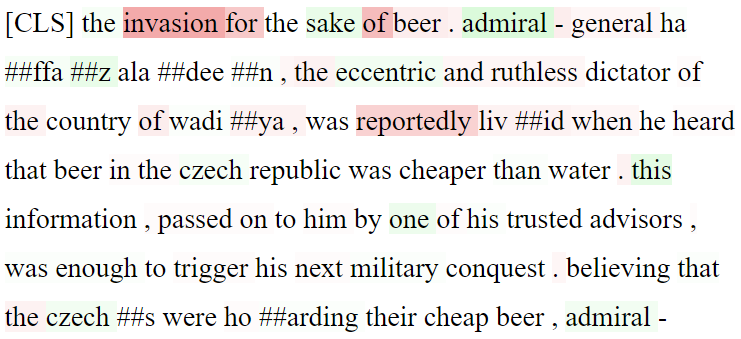
\includegraphics[width=\linewidth]{obrazky-figures/dictator.png}
      \caption{BERT model, correctly classified}
      \label{fig:apend1_a}
    \end{subfigure}%
    \begin{subfigure}{.5\textwidth}
      \centering
      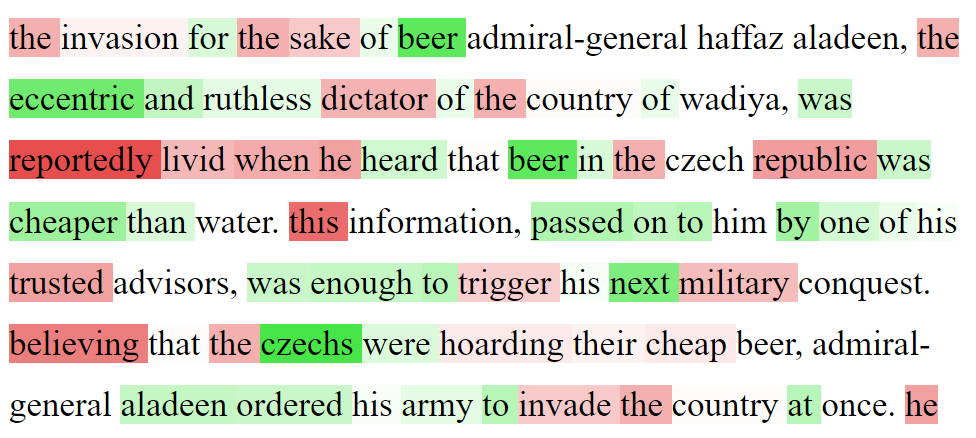
\includegraphics[width=\linewidth]{obrazky-figures/bayes_dictator.png}
      \caption{Baseline model, correctly classified}
      \label{fig:apend1_b}
    \end{subfigure}
    \caption{Interpretability of an unreliable article with the topic of war generated by ChatGPT.}
    \label{fig:apend1}
\end{figure}

Figure \ref{fig:apend1_b} shows an article about North Korea firing ballistic missiles into the sea from a reliable source. Figure \ref{fig:apend2_b} is an unreliable article stating that the covid vaccine is dangerous.


\begin{figure}[H]
    \centering
    \begin{subfigure}{.5\textwidth}
      \centering
      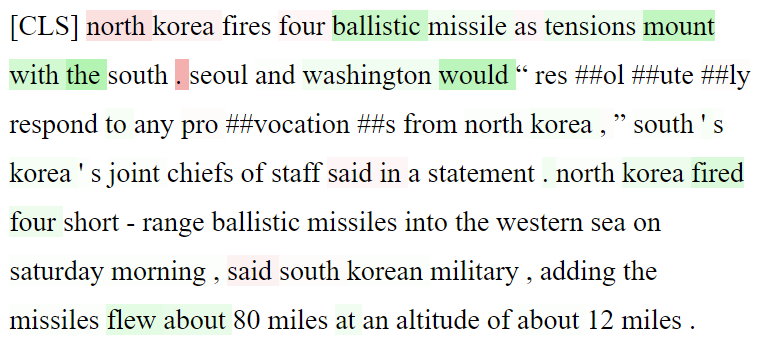
\includegraphics[width=\linewidth]{obrazky-figures/korea_weird.png}
      \caption{Label: reliable, topic: war \\result: correctly classified}
      \label{fig:apend2_a}
    \end{subfigure}%
    \begin{subfigure}{.5\textwidth}
      \centering
      \includegraphics[width=\linewidth]{obrazky-figures/covid2.png}
      \caption{Label: unreliable, topic: covid \\result: correctly classified}
      \label{fig:apend2_b}
    \end{subfigure}
    \caption{Interpretability for two articles by the BERT model.}
    \label{fig:apend2}
\end{figure}


\chapter{Contents of the Enclosed SD card}
The SD card enclosed as part of this thesis consists of the following tree structure: \\

\dirtree{%
    .1 /.
    .2 data \quad \ldots{} \begin{minipage}[t]{10cm}
                        Directory containing all datasets \\
                \end{minipage}.
    .2 src \quad \ldots{} \begin{minipage}[t]{10cm}
                        Directory containing all models and source files \\
                \end{minipage}.
    .3 tutorial.ipynb \ldots{} \begin{minipage}[t]{10cm}
                        This file contains a tutorial showing how to use the created models \\
                \end{minipage}.
    .2 src\_doc \ldots{} \begin{minipage}[t]{10cm}
                        Directory containing all source files of the latex documentation \\
                \end{minipage}.
    .2 doc \quad \ldots{} \begin{minipage}[t]{10cm}
                        Directory containing this pdf file \\
                \end{minipage}.
    .3 thesis{.}pdf \\.
    .2 requirements{.}txt \ldots{} \begin{minipage}[t]{10cm}
                        File containing all required libraries
                \end{minipage}.
}

  \else
    % Tento soubor nahraďte vlastním souborem s přílohami (nadpisy níže jsou pouze pro příklad)

% Umístění obsahu paměťového média do příloh je vhodné konzultovat s vedoucím
%\chapter{Obsah přiloženého paměťového média}

%\chapter{Manuál}

%\chapter{Konfigurační soubor}

%\chapter{RelaxNG Schéma konfiguračního souboru}

%\chapter{Plakát}

\chapter{Jak pracovat s touto šablonou}
\label{jak}

V této příloze je uveden popis jednotlivých částí šablony, po kterém následuje stručný návod, jak s touto šablonou pracovat. Pokud po jejím přečtení k šabloně budete mít nějaké dotazy, připomínky apod., neváhejte a napište na e-mail \texttt{sablona@fit.vutbr.cz}.

\section*{Popis částí šablony}

Po rozbalení šablony naleznete následující soubory a adresáře:
\begin{DESCRIPTION}
  \item [bib-styles] Styly literatury (viz níže). 
  \item [obrazky-figures] Adresář pro Vaše obrázky. Nyní obsahuje \texttt{placeholder.pdf} (tzv. TODO obrázek, který lze použít jako pomůcku při tvorbě technické zprávy), který se s prací neodevzdává. Název adresáře je vhodné zkrátit, aby byl jen ve zvoleném jazyce.
  \item [template-fig] Obrázky šablony (znak VUT).
  \item [fitthesis.cls] Šablona (definice vzhledu).
  \item [Makefile] Makefile pro překlad, počítání normostran, sbalení apod. (viz níže).
  \item [projekt-01-kapitoly-chapters.tex] Soubor pro Váš text (obsah nahraďte).
  \item [projekt-20-literatura-bibliography.bib] Seznam literatury (viz níže).
  \item [projekt-30-prilohy-appendices.tex] Soubor pro přílohy (obsah nahraďte).
  \item [projekt.tex] Hlavní soubor práce -- definice formálních částí.
\end{DESCRIPTION}

Styl literatury v šabloně je od Ing. Radka Pyšného \cite{Pysny}, jehož práce byla vylepšena prof. Adamem Heroutem, dr. Jaroslavem Dytrychem a panem Karlem Hanákem tak, aby odpovídala normě a podporovala všechny často využívané typy citací. Jeho dokumentaci naleznete v příloze \ref{priloha-priklady-citaci}.

\begin{samepage}
Makefile kromě překladu do PDF nabízí i další funkce:
\begin{itemize}
  \item přejmenování souborů (viz níže),
  \item počítání normostran,
  \item spuštění vlny pro doplnění nezlomitelných mezer,
  \item sbalení výsledku pro odeslání vedoucímu ke kontrole (zkontrolujte, zda sbalí všechny Vámi přidané soubory, a případně doplňte).
\end{itemize}
\end{samepage}

Nezapomeňte, že vlna neřeší všechny nezlomitelné mezery. Vždy je třeba manuální kontrola, zda na konci řádku nezůstalo něco nevhodného -- viz Internetová jazyková příručka\footnote{Internetová jazyková příručka \url{http://prirucka.ujc.cas.cz/?id=880}}.

\paragraph {Pozor na číslování stránek!} Pokud má obsah 2 strany a na 2. jsou jen \uv{Přílohy} a~\uv{Seznam příloh} (ale žádná příloha tam není), z nějakého důvodu se posune číslování stránek o 1 (obsah \uv{nesedí}). Stejný efekt má, když je na 2. či 3. stránce obsahu jen \uv{Literatura} a~je možné, že tohoto problému lze dosáhnout i jinak. Řešení je několik (od~úpravy obsahu, přes nastavení počítadla až po sofistikovanější metody). \textbf{Před odevzdáním proto vždy překontrolujte číslování stran!}


\section*{Doporučený postup práce se šablonou}

\begin{enumerate}
  \item \textbf{Zkontrolujte, zda máte aktuální verzi šablony.} Máte-li šablonu z předchozího roku, na stránkách fakulty již může být novější verze šablony s~aktualizovanými informacemi, opravenými chybami apod.
  \item \textbf{Zvolte si jazyk}, ve kterém budete psát svoji technickou zprávu (česky, slovensky nebo anglicky) a svoji volbu konzultujte s vedoucím práce (nebyla-li dohodnuta předem). Pokud Vámi zvoleným jazykem technické zprávy není čeština, nastavte příslušný parametr šablony v souboru projekt.tex (např.: \verb|document|\verb|class[english]{fitthesis}| a přeložte prohlášení a poděkování do~angličtiny či slovenštiny.
  \item \textbf{Přejmenujte soubory.} Po rozbalení je v šabloně soubor \texttt{projekt.tex}. Pokud jej přeložíte, vznikne PDF s technickou zprávou pojmenované \texttt{projekt.pdf}. Když vedoucímu více studentů pošle \texttt{projekt.pdf} ke kontrole, musí je pracně přejmenovávat. Proto je vždy vhodné tento soubor přejmenovat tak, aby obsahoval Váš login a (případně zkrácené) téma práce. Vyhněte se však použití mezer, diakritiky a speciálních znaků. Vhodný název může být např.: \uv{\texttt{xlogin00-Cisteni-a-extrakce-textu.tex}}. K přejmenování můžete využít i přiložený Makefile:
\begin{verbatim}
make rename NAME=xlogin00-Cisteni-a-extrakce-textu
\end{verbatim}
  \item Vyplňte požadované položky v souboru, který byl původně pojmenován \texttt{projekt.tex}, tedy typ, rok (odevzdání), název práce, svoje jméno, ústav (dle zadání), tituly a~jméno vedoucího, abstrakt, klíčová slova a další formální náležitosti.
  \item Nahraďte obsah souborů s kapitolami práce, literaturou a přílohami obsahem svojí technické zprávy. Jednotlivé přílohy či kapitoly práce může být výhodné uložit do~samostatných souborů -- rozhodnete-li se pro toto řešení, je doporučeno zachovat konvenci pro názvy souborů, přičemž za číslem bude následovat název kapitoly. 
  \item Nepotřebujete-li přílohy, zakomentujte příslušnou část v \texttt{projekt.tex} a příslušný soubor vyprázdněte či smažte. Nesnažte se prosím vymyslet nějakou neúčelnou přílohu jen proto, aby daný soubor bylo čím naplnit. Vhodnou přílohou může být obsah přiloženého paměťového média.
  \item Smažte soubory s kapitolami a přílohami pro jazyk, který jste nevyužili (s nebo bez \texttt{-en}).
  \item Zadání, které si stáhnete v PDF z IS FIT (odkaz \uv{Zadání pro vložení do práce} či \uv{Thesis assignment}), uložte do souboru \texttt{zadani.pdf} a povolte jeho vložení do práce parametrem šablony v \texttt{projekt.tex} (\verb|document|\verb|class[zadani]{fitthesis}|).
  \item Nechcete-li odkazy tisknout barevně (bez konzultace s vedoucím příliš nedoporučuji), budete pro tisk vytvářet druhé PDF s tím, že nastavíte parametr šablony pro tisk: (\verb|document|\verb|class[zadani,print]{fitthesis}|). Budete-li tisknout barevně, místo \texttt{print} použijte parametr \texttt{cprint}. Barevné logo se nesmí tisknout černobíle!
  \item Vzor desek, do kterých bude práce vyvázána, si vygenerujte v informačním systému fakulty u zadání. Pro disertační práci lze zapnout parametrem v šabloně \texttt{cover} (více naleznete v souboru \texttt{fitthesis.cls}).
  \item Nezapomeňte, že zdrojové soubory i (obě verze) PDF musíte odevzdat na CD či jiném médiu přiloženém k technické zprávě.
\end{enumerate}

Obsah práce se generuje standardním příkazem \tt \textbackslash tableofcontents \rm (zahrnut v šabloně). Přílohy jsou v něm uvedeny úmyslně.

\subsection*{Pokyny pro oboustranný tisk}
\begin{itemize}
\item \textbf{Oboustranný tisk je doporučeno konzultovat s vedoucím práce.}
\item Je-li práce tištěna oboustranně a její tloušťka je menší než tloušťka desek, nevypadá to dobře.
\item Zapíná se parametrem šablony: \verb|\document|\verb|class[twoside]{fitthesis}|
\item Po vytištění oboustranného listu zkontrolujte, zda je při prosvícení sazební obrazec na obou stranách na stejné pozici. Méně kvalitní tiskárny s duplexní jednotkou mají často posun o 1--3 mm. Toto může být u některých tiskáren řešitelné tak, že vytisknete nejprve liché stránky, pak je dáte do stejného zásobníku a vytisknete sudé.
\item Za titulním listem, obsahem, literaturou, úvodním listem příloh, seznamem příloh a případnými dalšími seznamy je třeba nechat volnou stránku, aby následující část začínala na liché stránce (\texttt{\textbackslash cleardoublepage}).
\item  Konečný výsledek je nutné pečlivě překontrolovat.
\end{itemize}

\subsection*{Styl odstavců}

Odstavce se zarovnávají do bloku a pro jejich formátování existuje více metod. U papírové literatury je častá metoda s~použitím odstavcové zarážky, kdy se u~jednotlivých odstavců textu odsazuje první řádek odstavce asi o~jeden až dva čtverčíky, tedy přibližně o~dvě šířky velkého písmene M základního textu (vždy o~stejnou, předem zvolenou hodnotu). Poslední řádek předchozího odstavce a~první řádek následujícího odstavce se v~takovém případě neoddělují svislou mezerou. Proklad mezi těmito řádky je stejný jako proklad mezi řádky uvnitř odstavce \cite{fitWeb}.

Další metodou je odsazení odstavců, které je časté u elektronické sazby textů. První řádek odstavce se při této metodě neodsazuje a mezi odstavce se vkládá vertikální mezera o~velikosti 1/2 řádku. Obě metody lze v kvalifikační práci použít, nicméně často je vhodnější druhá z uvedených metod. Metody není vhodné kombinovat.

Jeden z výše uvedených způsobů je v šabloně nastaven jako výchozí, druhý můžete zvolit parametrem šablony \uv{\tt odsaz\rm }.

\subsection*{Užitečné nástroje}
\label{nastroje}

Následující seznam není výčtem všech využitelných nástrojů. Máte-li vyzkoušený osvědčený nástroj, neváhejte jej využít. Pokud však nevíte, který nástroj si zvolit, můžete zvážit některý z následujících:

\begin{description}
	\item[\href{http://miktex.org/download}{MikTeX}] \LaTeX{} pro Windows -- distribuce s jednoduchou instalací a vynikající automatizací stahování balíčků. MikTex obsahuje i vlastní editor, ale spíše doporučuji TeXstudio.
	\item[\href{http://texstudio.sourceforge.net/}{TeXstudio}] Přenositelné GUI pro \LaTeX{} s otevřeným zdrojovým kódem (opensource).  Ctrl+klik umožňuje přepínat mezi zdrojovým textem a PDF. Má integrovanou kontrolu pravopisu\footnote{Českou kontrolu pravopisu lze doinstalovat z \url{https://extensions.openoffice.org/de/project/czech-dictionary-pack-ceske-slovniky-cs-cz}}, zvýraznění syntaxe apod. Pro jeho využití je nejprve potřeba nainstalovat MikTeX, případně jinou \LaTeX ovou distribuci.
	\item[\href{http://www.winedt.com/}{WinEdt}] Ve Windows je dobrá kombinace WinEdt + MiKTeX. WinEdt je GUI pro Windows, pro jehož využití je nejprve potřeba nainstalovat \href{http://miktex.org/download}{MikTeX} či \href{http://www.tug.org/texlive/}{TeX Live}. 
	\item[\href{http://kile.sourceforge.net/}{Kile}] Editor pro desktopové prostředí KDE (Linux). Umožňuje živé zobrazení náhledu. Pro jeho využití je potřeba mít nainstalovaný \href{http://www.tug.org/texlive/}{TeX Live} a Okular. 
	\item[\href{http://jabref.sourceforge.net/download.php}{JabRef}] Pěkný a jednoduchý program v Javě pro správu souborů s bibliografií (literaturou). Není potřeba se nic učit -- poskytuje jednoduché okno a formulář pro editaci položek.
	\item[\href{https://inkscape.org/en/download/}{InkScape}] Přenositelný opensource editor vektorové grafiky (SVG i PDF). Vynikající nástroj pro tvorbu obrázků do odborného textu. Jeho ovládnutí je obtížnější, ale výsledky stojí za to.
	\item[\href{https://git-scm.com/}{GIT}] Vynikající pro týmovou spolupráci na projektech, ale může výrazně pomoci i jednomu autorovi. Umožňuje jednoduché verzování, zálohování a přenášení mezi více počítači.
	\item[\href{http://www.overleaf.com/}{Overleaf}] Online nástroj pro \LaTeX{}. Přímo zobrazuje náhled a umožňuje jednoduchou spolupráci (vedoucí může průběžně sledovat psaní práce), vyhledávání ve zdrojovém textu či ve vygenerovaném PDF, kontrolu pravopisu apod. Zdarma jej však lze využít pouze s určitými omezeními (někomu stačí na disertaci, jiný na ně může narazit i při psaní bakalářské práce) a pro dlouhé texty je pomalejší. FIT VUT v Brně má pro studenty i~zaměstnance licenci, kterou si lze aktivovat na \url{https://www.overleaf.com/edu/but}.
\end{description}

Pozn.: Overleaf nepoužívá Makefile v šabloně -- aby překlad fungoval, je v menu nutné zvolit \tt projekt.tex \rm jako hlavní dokument.

\chapter{Psaní anglického textu}
\label{anglicky}
Tato příloha je převzata ze stránek doc. Černockého \cite{CernockyEnglish}.

Spousta lidí píše zprávy k projektům anglicky (a to je dobře!), ale dělá v nich spoustu zbytečných chyb (a to je špatně). Nejsem angličtinář, ale tento jazyk už nějakých pár let používám k psaní, čtení i komunikaci -- tato příloha obsahuje pár důležitých věcí. Pokud chcete napsat práci nebo článek opravdu 100\,\% dobře, nezbude Vám než si najmout rodilého mluvčího (a to by měl by být trochu technicky zdatný a aspoň trochu rozumět tomu, co píšete, ať to neskončí ještě hůř \ldots).

\section*{Obecně}

\begin{itemize}
  \item{Předtím, než budete sami něco psát, si přečtěte pár anglických technických článků a~zkuste si zapamatovat a získat \uv{obecný pocit}, jak se to píše.}
  \item{Používejte vždy korektor pravopisu -- zabudovaný ve Wordu, nebo v OpenOffice, pokud děláte na Linuxu, tak ISPELL a další (většina editorů pro \LaTeX{} má již kontrolu pravopisu integrovanou).}
  \item{Používejte korektor gramatiky. Nevím, jestli je nějaký dostupný na Linuxu, ale ten ve Wordu celkem slušně funguje a pokud Vám něco zelené podtrhne, je tam většinou opravdu chyba. Můžete do něj nakopírovat i zdrojový text pro \LaTeX{}, opravit, a pak uložit opět jako čistý text. Pokud používáte vim, je tam zabudovaný také a zvládne jak překlepy, tak základní gramatiku. V dokumentu \texttt{diplomka.tex} na první řádek napište: 
  \begin{verbatim}
    % vim:spelllang=en_us:spell
  \end{verbatim}
  (případně \texttt{en\_gb} pro OED angličtinu)
  \textit{Poznámka editora:} Existuje i velmi dobrý online nástroj Grammarly\footnote{\url{https://www.grammarly.com/}}, který je v základní verzi zdarma. 
  }
  \item{Online slovníky jsou dobré, ale nepoužívejte je slepě. Většinou dají více variant a ne každá je správně.}
  \item{\begin{samepage}Na vyhledávání a zjištění, co bude asi správné, můžete použít Google. Např.: nevíte, jak se řekne \uv{výhoda tohoto přístupu}. Slovník na seznam.cz dá asi 10 variant. Napište je postupně do vyhledávání na googlu:
  \begin{verbatim}
    "advantage of this approach" 1100000 hits
    "privilege of this approach" 6 hits
    "facility of this approach"  16 hits
  \end{verbatim}
  Neříkám, že je to 100\,\% správně, ale je to určité vodítko. Toto se dá použít i~na~dohledání správných spojek (třeba \uv{among two cases} nebo \uv{between two cases}?)\end{samepage}}
\end{itemize}
       
\section*{SVOMPT a shoda}

Struktura anglické věty je SVOPMT: SUBJECT VERB OBJECT MANNER PLACE TIME a přes to nejede vlak! Není volná jako v češtině. Jinak to je maximálně v nějaké divadelní hře, kde je potřeba něco zdůraznit. Hlavně podmět tam musí vždy být, na to se často zapomíná, protože v CZ/SK může být zamlčený nebo nevyjádřený. SVOMPT platí i~ve vedlejších větách!
\begin{verbatim}
  BAD: We have shown that is faster than the other function. 
  GOOD: We have shown that it is faster than the other function. 
\end{verbatim}

\noindent Shoda podmětu s přísudkem -- zní to šíleně, ale dělá se v tom spousta chyb. 

\begin{verbatim}
  he has 
  the users have 
  people were 
\end{verbatim}

\section*{Členy}

Členy v angličtině jsou noční můra a téměř nikdo z nás je nedává dobře. Základní pravidlo je, že když je něco určitého, musí předtím být \uv{the}. Členy musí být určitě u těchto spojení:
\begin{verbatim}
  the first, the second, ...
  the last
  the most (třetí stupeň přídavných jmen a príslovcí) ...
  the whole 
  the following 
  the figure, the table. 
  the left, the right - on the left pannel, from the left to the right ... 
\end{verbatim}

\noindent Naopak člen NESMÍ být, pokud používáte přesné označení obrázku, kapitoly atd.
\begin{verbatim}
  in Figure 3.2
  in Chapter 7
  in Table 6.4
\end{verbatim}

\begin{samepage}
\noindent Pozor na \uv{a} vs. \uv{an}, řídí se to podle výslovnosti a ne podle toho, jak je slovo napsané, takže:
\begin{verbatim}
  an HMM
  an XML
  a universal model
  a user
\end{verbatim}
\end{samepage}

\section*{Slovesa}

Pozor na trpné tvary sloves -- u pravidelných je to většinou bez problémů, u nepravidelných často špatně, typicky
\begin{verbatim}
  packet was sent (ne send)
  approach was chosen (ne choosed)
\end{verbatim}
\noindent \ldots vetšinou to opraví korektor pravopisu, ale někdy ne. 

Pozor na časy, občas je v nich pěkný nepořádek. Pokud něco nějak obecně je, přítomný čas. Pokud jste něco udělali, minulý. Pokud to dalo nějaký výsledek a ten výsledek teď existuje a třeba ho nějak diskutujete, přítomný. Nepoužívejte příliš složité časy jako je předpřítomný a vůbec ne předminulý pokud nevíte přesně, co děláte.
\begin{verbatim}
  JFA is a technique that works for everyone in speaker recognition. 
  We implemented it according to Kenny's recipe in \cite{Kenny}. 
  12000 segments from NIST SRE 2006 were processed. When compared 
  with a GMM baseline, the results are completely bad. 
\end{verbatim}

\section*{Délka vět a struktura}

\begin{itemize}
  \item{Pište kratší věty a souvětí, pokud máte něco na 5 řádků, většinou se to nedá číst.}
  \item{Strukturujte věty pomocí čárek (více než v češtině!), hlavně po úvodu věty, po kterém začíná vlastní věta. Někdy se dává čárka i před \uv{and} (na rozdíl od češtiny).}
\end{itemize}
\begin{verbatim}
  In this chapter, we will investigate ... 
  The first technique did not work, the second did not work as well, 
  and the third one also did not work. 
\end{verbatim}

\section*{Specifika technického textu}

Píšete technický text, proto nepoužívejte zkratky
\begin{verbatim}
  he's
  gonna
  Petr's working on ...
\end{verbatim}
\noindent a podobně. Jediné, které je tolerované, je \uv{doesn't}, ale neuděláte chybu, když napíšete \uv{does not}. 

\begin{samepage}
\noindent V technických textech se spíš používá trpný rod než činný: 
\begin{verbatim}
  BAD: In this chapter, I describe used programming languages. 
  GOOD: In this chapter, used programming languages are described.
\end{verbatim}
\end{samepage}

Pokud už činný použijete, dává se v technických textech spíše \uv{we}, i když na práci děláte sami. \uv{I}, \uv{my} atd. se používají pouze tam, kde jde o to zdůraznit, že jde o Vaši osobu, tedy třeba v závěru nebo v popisu \uv{original claims} v disertaci.

\paragraph{Časté chyby ve slovech}

\begin{itemize}
  \item{Pozor na jeho/její, není to it's, ale its.}
  \item{Obrázek není picture, ale figure. }
  \item{Spojka \uv{než} je \uv{than}, ne \uv{then} -- bigger than this, smaller than this \ldots hrozně častá chyba! \uv{Then} je pak, potom.}
\end{itemize}


\chapter{Checklist} 
\label{checklist}
Tento checklist byl převzat ze šablony pro kvalifikační práce, která je k dispozici na blogu prof. Herouta \cite{Herout}, který s laskavým dovolením využil nápadu dr. Szökeho%
\footnote{\url{http://blog.igor.szoke.cz/2017/04/predstartovni-priprava-letu-neni.html}}. 

Velká bezpečnost letecké dopravy stojí z části na tom, že lidé kolem letadel mají \textbf{checklisty} na úplně každý, třeba rutinní a dobře zažitý, postup. Jako pilot strpí to, že bude trochu za blbce a opravdu tužtičkou do seznamu úkonů odškrtá dokonale zvládnuté akce, vytiskněte si a odškrtejte před odevzdáním diplomky i vy tento checklist a vyhněte se tak častým chybám, které by mohly mít až fatální následky na výsledné hodnocení Vaší práce.

\subsubsection*{Struktura}
\begin{checklist}
	\item Už ze samotných názvů a struktury kapitol je patrné, že bylo splněno zadání.
	\item V textu se nevyskytuje kapitola, která by měla méně než čtyři strany (kromě úvodu a závěru). Pokud ano, radil(a) jsem se o tom s vedoucím a ten to schválil.
\end{checklist}

\subsubsection*{Obrázky a grafy}
\begin{checklist}
	\item Všechny obrázky a tabulky byly zkontrolovány a jsou poblíž místa, odkud jsou z textu odkazovány, takže nebude problém je najít.
	\item Všechny obrázky a tabulky mají takový popisek, že celý obrázek dává smysl sám o~sobě, bez čtení dalšího textu. Vůbec nevadí, když má popisek několik řádků.
	\item Pokud je obrázek převzatý, tak je to v popisku zmíněno: \uv{Převzato z [X].}
	\item Písmenka ve všech obrázcích používají font podobné velikosti, jako je okolní text (ani výrazně větší, ani výrazně menší).
	\item Grafy a schémata jsou vektorově (tj. v PDF).
	\item Snímky obrazovky nepoužívají ztrátovou kompresi (jsou v PNG).
	\item Všechny obrázky jsou odkázány z textu.
	\item Grafy mají popsané osy (název osy, jednotky, hodnoty) a podle potřeby mřížku.
\end{checklist}

\subsubsection*{Rovnice}
\begin{checklist}
	\item Identifikátory a jejich indexy v rovnicích jsou jednopísmenné (kromě nečastých zvláštních případů jako $t_\mathrm{max}$).
	\item Rovnice jsou číslovány.
	\item Za (nebo vzácně před) rovnicí jsou vysvětleny všechny proměnné a funkce, které zatím vysvětleny nebyly.
\end{checklist}

\subsubsection*{Citace}
\begin{checklist}
    \item \textbf{Všechny použité zdroje jsou citovány.}
	\item Adresy URL odkazující na služby, projekty, zdroje, github apod. jsou odkazovány pomocí \verb|\footnote{\url{...}}|.
    \item Všechny citace používají správné typy.
	\item Citace mají autora, název, vydavatele (název konference), rok vydání.  Když některá nemá, je to dobře zdůvodněný zvláštní případ a vedoucí to odsouhlasil.
	\item Je-li ve zdrojových textech programu něco převzaté, je to tam řádně citováno v souladu s licencí.
	\item Je-li podstatná část zdrojových textů programu převzatá, je toto zmíněno v textu práce a je citován zdroj.
\end{checklist}

\subsubsection*{Typografie}
\begin{checklist}
	\item Žádný řádek nepřetéká přes pravý okraj.
	\item Na konci řádku nikde není jednopísmenná předložka (spraví to nedělitelná mezera $\sim$).
	\item Číslo obrázku, tabulky, rovnice, citace není nikde první na novém řádku (spraví to nedělitelná mezera $\sim$).
	\item Před číselným odkazem na poznámku pod čarou nikde není mezera (to jest vždy takto\footnote{příklad poznámky pod čarou}, nikoliv takto \footnote{jiný příklad poznámky pod čarou}).
\end{checklist}

\subsubsection*{Jazyk}
\begin{checklist}
    \item Použil jsem kontrolu pravopisu a v textu nikde nejsou překlepy.
	\item Nechal jsem si text přečíst od (alespoň) jednoho dalšího člověka, který umí dobře česky / anglicky / slovensky.
	\item V práci psané česky nebo slovensky abstrakt zkontroloval někdo, kdo umí opravdu dobře anglicky.
	\item V textu se nikde nepoužívá druhá mluvnická osoba (vy/ty).
	\item Když se v textu vyskytuje první mluvnická osoba (já, my), vždy se popisuje subjektivní záležitost (\textit{rozhodl jsem se}, \textit{navrhl jsem}, \textit{zaměřil jsem se na}, \textit{zjistil jsem} apod.).
	\item V textu se nikde nepoužívají hovorové výrazy.
	\item V českém či slovenském textu se zbytečně nepoužívají anglické výrazy, které mají ustálené české překlady. Např. slovo \textit{defaultní} se nahradí např. slovem \textit{implicitní} nebo \textit{výchozí}.
\end{checklist}

\subsubsection*{Výsledek na datovém médiu, tj. software}
\begin{checklist}
	\item Mám připravené nepřepisovatelné datové médium 
      \begin{itemize}
	  		\item CD-R,
            \item DVD-R,
            \item DVD+R ve formátu ISO9660 (s rozšířením RockRidge a/nebo Jolliet) nebo UDF,
            \item paměťová karta SD (Secure Digital) ve formátu FAT32 nebo exFAT s nastavenou ochranou proti přepisu.
      \end{itemize}
	\item Pokud je výsledek online (služba, aplikace, \dots), URL je viditelně v úvodu a závěru, aby bylo jasné, kde výsledek hledat.
	\item Na médiu nechybí povinné: 
    	\begin{itemize}
    		\item zdrojové kódy (např. Matlab, C/C++, Python, \dots)
            \item knihovny potřebné pro překlad,
            \item přeložené řešení,
            \item PDF s technickou zprávou (je-li pro tisk 2. verze, tak obě),
            \item zdrojový kód zprávy (\LaTeX), 
    	\end{itemize}
        a případně volitelně po dohodě s vedoucím práce
		\begin{itemize}
			\item relevantní (např. testovací) data, 
            \item demonstrační video,
            \item PDF plakátku,
            \item \dots
		\end{itemize}        
	\item Zdrojové kódy jsou refaktorovány, komentovány a označeny hlavičkou s autorstvím, takže se v nich snadno vyzná i někdo další, než sám autor.
    \item Jakákoliv převzatá část zdrojového kódu je řádně citována -- tedy označena úvodním a v případě převzetí více řádků i ukončovacím komentářem. Komentář obsahuje vše, co vyžaduje licence uvedená na webu (vždy je nutné se ji pokusit najít -- např. Stack Overflow\footnote{\url{https://stackoverflow.blog/2009/06/25/attribution-required/}} má striktní pravidla pro citace).
\end{checklist}

\subsubsection*{Odevzdání}

\begin{checklist}
\item Chci práci (na max. 3 roky) utajit? Pokud ano, nejpozději měsíc před termínem odevzdání práce si podám žádost (v IS), ke které přiložím případné stanovisko firmy, jejíž duševní vlastnictví je třeba chránit.
\item Mám splněný minimální počet normostran textu (lze spočítat pomocí Makefile a~odhadem přičíst obrázky). Pokud jsem těsně pod minimem, konzultoval(a) jsem to s~vedoucím.
\item Pokud chci tisknout oboustranně, konzultoval(a) jsem to s~vedoucím a mám správně nastavenou šablonu. Kapitoly začínají na liché stránce.
\item Technickou zprávu mám v deskách z knihařství (min. 1 výtisk, při utajení oba).
\item Za titulním listem práce je zadání (tzn. mám jej stažené z IS a vložené do šablony).
\item V IS jsou abstrakty a klíčová slova.
  \begin{itemize}
    \item V abstraktu a klíčových slovech v IS nejsou zkopírované vlnky pro nezlomitelné mezery.
  \end{itemize}      
\item V IS je PDF práce (s klikatelnými odkazy).
\item Oba výtisky práce jsou podepsané.
\item V jednom (při utajení obou) výtisku práce je paměťové médium, na kterém je fixkou napsaný login (fixku na CD lze zapůjčit v knihovně, na Studijním oddělení nebo až při odevzdání).
\end{checklist}


\chapter{\LaTeX pro začátečníky}
\label{latex}

V této kapitole jsou uvedeny některé často využívané balíčky a příkazy pro \LaTeX{}, které mohou být při tvorbě práce potřeba.

\subsection*{Užitečné balíčky}

Studenti při sazbě textu často řeší stejné problémy. Některé z nich lze vyřešit následujícími balíčky pro \LaTeX:

\begin{itemize}
  \item \verb|amsmath| -- rozšířené možnosti sazby rovnic,
  \item \verb|float, afterpage, placeins| -- úprava umístění obrázků/tabulek (specifikátor \texttt{H}),
  \item \verb|fancyvrb, alltt| -- úpravy vlastností prostředí Verbatim, 
  \item \verb|makecell| -- rozšíření možností tabulek,
  \item \verb|pdflscape, rotating| -- natočení stránky o 90 stupňů (pro obrázek či tabulku),
  \item \verb|hyphenat| -- úpravy dělení slov,
  \item \verb|picture, epic, eepic| -- přímé kreslení obrázků.
\end{itemize}

Některé balíčky jsou využity přímo v šabloně (v dolní části souboru \texttt{fitthesis.cls}). Nahlédnutí do jejich dokumentace může být rovněž velmi užitečné.

Sloupec tabulky zarovnaný vlevo s pevnou šířkou je v šabloně definovaný \uv{L} (používá se jako \uv{p}).

Pro odkazování v rámci textu použijte příkaz \verb|\ref{navesti}|. Podle umístění návěští se bude jednat o~číslo kapitoly, podkapitoly, obrázku, tabulky nebo podobného číslovaného prvku). Pokud chcete odkázat stránku práce, použijte příkaz \verb|pageref{navesti}|. Pro citaci literárního odkazu \verb|\cite{identifikator}|. Pro odkazy na rovnice lze použít příkaz \verb|\eqref{navesti}|.

Znak \,--\, (pomlčka) se V \LaTeX u vkládá jako dvě mínus za sebou: -{}-.

\subsection*{Často využívané příkazy pro \LaTeX{}}
\label{sec:Fragments}

Doporučuji nahlédnout do zdrojového textu této podkapitoly a podívat se, jak jsou následující ukázky vysázeny. Ve zdrojovém textu jsou i pomocné komentáře.

% Sloupec zarovnaný vlevo s pevnou šířkou je v šabloně definovaný "L" (používá se jako p)

Příklad tabulky:
\begin{table}[H]
	\vskip6pt
	\caption{Tabulka hodnocení} 
    \vskip6pt
	\centering
	\begin{tabular}{llr}
		\toprule
		\multicolumn{2}{c}{Jméno} \\
		\cmidrule(r){1-2}
		Jméno & Příjmení & Hodnocení \\
		\midrule
		Jan & Novák & $7.5$ \\
		Petr & Novák & $2$ \\
		\bottomrule
	\end{tabular}
	\label{tab:ExampleTable}
\end{table}

% Ohraničení lze upravit dle potřeby:
% http://latex-community.org/forum/viewtopic.php?f=45&t=24323
% http://tex.stackexchange.com/questions/58163/problem-with-multirow-and-table-cell-borders
% http://tex.stackexchange.com/questions/79369/formatting-table-border-and-text-alignment-in-latex-table

\noindent Příklad rovnice:
\begin{equation}
	\cos^3 \theta =\frac{1}{4}\cos\theta+\frac{3}{4}\cos 3\theta
	\label{eq:rovnice2}
\end{equation}
a dvou horizontálně zarovnaných rovnic: % znak & řídí zarovnání
\begin{align} 
    \label{eq:soustava}
	3x &= 6y + 12 \\
	x &= 2y + 4 
\end{align}

Pokud je třeba rovnici citovat v textu, lze použít příkaz \verb|\eqref|. Například na rovnici výše lze odkázat~\eqref{eq:rovnice2}. Pokud chcete srovnat číslo rovnic u soustavy, lze použít prostředí \texttt{split}:
\begin{equation} \label{eq:soustavaSrovnana}
\begin{split}
	3x &= 6y + 12 \\
	x &= 2y + 4
\end{split}
\end{equation}

Matematické symboly ($\alpha$) a výrazy lze umístit i do textu $\cos\pi=-1$ a mohou být i~v~poznámce pod čarou%
\footnote{Vzorec v poznámce pod čarou: $\cos\pi=-1$}.

Obrázek~\ref{sirokyObrazek} ukazuje široký obrázek složený z více menších obrázků. Klasický rastrový obrázek se vkládá tak, jak je vidět na obrázku \ref{keepCalm}.

% Využití \begin{figure*} způsobí, že obrázek zabere celou šířku stránky. Takový obrázek dříve mohl být pouze na začátku stránky, případně na konci s využitím balíčku dblfloatfix (případné [h] se ignorovalo a [H] obrázek odstraní). Nové verze LaTeXu už umí i [h].
\begin{figure*}[h]\centering
  \centering
  \includegraphics[width=\linewidth,height=1.7in]{obrazky-figures/placeholder.pdf}\\[1pt]
  \includegraphics[width=0.24\linewidth]{obrazky-figures/placeholder.pdf}\hfill
  \includegraphics[width=0.24\linewidth]{obrazky-figures/placeholder.pdf}\hfill
  \includegraphics[width=0.24\linewidth]{obrazky-figures/placeholder.pdf}\hfill
  \includegraphics[width=0.24\linewidth]{obrazky-figures/placeholder.pdf}
  \caption{\textbf{Široký obrázek.} Obrázek může být složen z více menších obrázků. Chcete-li se na tyto dílčí obrázky odkazovat z textu, využijte balíček \texttt{subcaption}.}
  \label{sirokyObrazek}
\end{figure*}

% Odkomentujte pro přepnutí na formát A3 na šířku
% \eject \pdfpagewidth=420mm

\begin{figure}[hbt]
	\centering
	\includegraphics[width=0.3\textwidth]{obrazky-figures/keep-calm.png}
	\caption{Dobrý text je špatným textem, který byl několikrát přepsán. Nebojte se prostě něčím začít.}
	\label{keepCalm}
\end{figure}

Někdy je potřeba do příloh umístit diagram, který se nevejde na stránku formátu A4. Pak je možné vložit jednu stránku formátu A3 a do práce ji poskládat (tzv. skládání do~Z, kdy se vytvoří dva sklady -- lícem dolů a lícem nahoru, angl. Engineering fold -- existuje i~anglický pojem Z-fold, ale při tom by byl problém s vazbou). Přepnutí se provádí následovně: \texttt{\textbackslash{}eject \textbackslash{}pdfpagewidth=420mm} (pro přepnutí zpět pak 210mm).

Další často využívané příkazy naleznete ve zdrojovém textu ukázkového obsahu této šablony.

% Odkomentujte pro přepnutí zpět na A4
% \eject \pdfpagewidth=210mm


\newcommand{\odradkovani}{\\[0.3em]}

\chapter{Příklady bibliografických citací}
\label{priloha-priklady-citaci}
Styl czplain vychází ze stylu vytvořeného v rámci práce pana Pyšného \cite{Pysny}. Obsahuje sadu podporovaných typů citací s konkrétními příklady bibliografických citací. 

Na následujících stránkách přílohy jsou uvedeny příklady, jenž znázorňují bibliografické citace následujících publikací a~jejich částí:
\begin{itemize}
   \item článku v seriálové publikaci (časopisu) (str. \pageref{pr-casopis-clanek}),
   \item monografické publikace (str. \pageref{pr-monografie}),
   \item sborníku (str. \pageref{pr-sbornik}),
   \item článku ve sborníku nebo kapitoly v knize (str. \pageref{pr-kapitola}),
   \item manuálu, dokumentace, technické zprávy a nepublikovaných materiálů (str. \pageref{pr-manual}),
   \item akademické práce (str. \pageref{pr-thesis}),
   \item webové stránky (str. \pageref{pr-webpage}),
   \item a webové domény (str. \pageref{pr-website}).
\end{itemize}

\noindent Položky jsou označený barevně podle povinnosti:
\begin{itemize}
    \item prvek je dle normy povinný
    \item \textcolor{blue}{prvek, který je dle normy volitelný}
    \item \textcolor{magenta}{prvek, který je dle normy povinný pro online informační zdroje}
    \item \textcolor{red}{prvek, který není předepsán normou a je v bibliografickém stylu v šabloně volitelný}
\end{itemize}
Povinné položky se uvádí pouze pokud existují.

\newpage
\noindent V souboru s bibliografií se záznamy uvádí následujícím způsobem:
\begin{verbatim}
@Article{Doe:2020,
   author               = "Doe, John",
   title                = "Jak citovat",
   subtitle             = "Citace článku",
   journal              = "Seriál o tvorbě prací",
   journalsubtitle      = "Formální náležitosti",
   howpublished         = "online",
   address              = "Brno",
   publisher            = "Fakulta informačních technologií VUT v Brně",
   contributory         = "Přeložil Jan NOVÁK",
   edition              = "1",
   version              = "verze 1.0",
   month                = 2,
   year                 = "2020",
   revised              = "revidováno 12. 2. 2020",
   volume               = "4",
   number               = "24",
   pages                = "8--21",
   cited                = "2020-02-12",
   doi                  = "10.1000/BC1.0",
   issn                 = "1234-5678",
   note                 = "Toto je zcela vymyšlená citace",
   url                  = "https://merlin.fit.vutbr.cz"
}
\end{verbatim}

Citace jsou seřazeny podle abecedy. Řazení jmen s písmeny s diakritikou můžeme ovlivnit prvkem \texttt{key}, jehož  hodnotu nastavíme na příjmení bez diakritiky. Pokud není vyplněn autor, citace se řadí na začátek seznamu, což není vhodné. Řazení v tomto případě můžeme taktéž ovlivnit vhodně nastaveným prvkem key.

\medskip
\medskip
\noindent \textbf{Příklad}:
\begin{verbatim}
   @Article{Cech:2020:Citace,
	   author               = "Čech, Jan",
	   key                  = "Cech",
	   ... 
\end{verbatim}


%-------------------------------------------------------------------------------
\newpage
\section*{Článek v seriálové publikaci - @Article}
\label{pr-casopis-clanek}
\noindent \textbf{Položky záznamu}

\medskip

\begin{tabularx}{\linewidth}{X X X}
    Prvek & Zápis v BibTeXu & Příklad \\\hline
    Tvůrce & author & Doe, John\\
    Název příspěvku & title & Jak citovat\\
    \textcolor{blue}{Vedlejší název} & \textcolor{blue}{subtitle} & \textcolor{blue}{Citace článku}\\
    Název seriálové publikace & journal & Seriál o tvorbě prací\\
    \textcolor{blue}{Vedlejší názvy seriálu} & \textcolor{blue}{journalsubtitle} & \textcolor{blue}{Formální náležitosti}\\
    \textcolor{magenta}{Typ nosiče} & \textcolor{magenta}{howpublished} & \textcolor{magenta}{online}\\
    Vydání & edition & 1\\
    Verze & version & verze 1.0\\
    \textcolor{blue}{Další tvůrce} & \textcolor{blue}{contributory} & \textcolor{blue}{Přeložil Jan NOVÁK}\\
    Místo vydání & address & Brno\\
    Nakladatel & publisher & Fakulta informačních technologií VUT v Brně\\
    Měsíc & month & 2\\
    Rok & year & 2020\\
    Svazek & volume & 4\\
    Číslo & number & 24\\
    Rozsah příspěvku & pages & 8-21\\
    Revize & revised & revidováno 12. 2. 2020\\
    \textcolor{magenta}{Datum citování} & \textcolor{magenta}{cited} & \textcolor{magenta}{2020-02-12}\\
    Název edice & series & Návody k tvorbě prací\\
    Číslo edice & editionnumber & 42\\
    \textcolor{magenta}{Identifikátor digitálního obsahu} & \textcolor{magenta}{doi} & \textcolor{magenta}{10.1000/BC1.0}\\
    Standardní číslo  & issn & 1234-5678\\
    \textcolor{red}{Poznámky} & \textcolor{red}{note} & \textcolor{red}{Toto je zcela vymyšlená citace}\\
    \textcolor{magenta}{Dostupnost a přístup} & \textcolor{magenta}{url} & \textcolor{magenta}{https://merlin.fit.vutbr.cz}
\end{tabularx}

\bigskip

\noindent \textbf{Bibliografická citace}

\medskip

\noindent \textsc{Doe}, J. Jak Citovat: Citace článku. \textit{Seriál o tvorbě prací: Formální náležitosti} [online]. 1. vyd., verze 1.0. Přeložil Jan NOVÁK. Brno: Fakulta informačních technologií VUT v Brně. Únor 2020, sv. 4, č. 24, s. 8–21, revidováno 12. 2. 2020, [cit. 2020-02-12]. Návody k tvorbě prací, č. 42. DOI: 10.1000/BC1.0. ISSN 1234-5678. Toto je zcela vymyšlená citace. Dostupné z: \url{https://merlin.fit.vutbr.cz}

%-------------------------------------------------------------------------------
\newpage
\section*{Monografická publikace - @Book, @Booklet (kniha, brožura)}
\label{pr-monografie}
\noindent \textbf{Položky záznamu}

\medskip

\begin{tabularx}{\linewidth}{X X X}
    Prvek & Zápis v BibTeXu & Příklad\\\hline
    Tvůrce & author & John von Doe\\
    Titul & title & Jak citovat\\
    \textcolor{blue}{Vedlejší názvy} & \textcolor{blue}{subtitle} & \textcolor{blue}{Citace monografické publikace}\\
    \textcolor{magenta}{Typ nosiče} & \textcolor{magenta}{howpublished} & \textcolor{magenta}{online}\\
    Vydání & edition & 1\\
    \textcolor{blue}{Další tvůrce} & \textcolor{blue}{contributory} & \textcolor{blue}{Přeložil Jan NOVÁK}\\
    Místo vydání & address & Brno\\
    Nakladatel & publisher & Fakulta informačních technologií VUT v Brně\\
    Měsíc vydání & month & 2\\
    Rok vydání & year & 2020\\
    Revize & revision & revidováno 12. 2. 2020\\
    \textcolor{magenta}{Datum citování} & \textcolor{magenta}{cited} & \textcolor{magenta}{2020-02-12}\\
    \textcolor{red}{Rozsah} & \textcolor{red}{pages} & \textcolor{red}{220}\\
    Edice & series & Návody k tvorbě prací\\
    Číslo edice & editionnumber & 2\\
    Standardní číslo & isbn & 01-234-5678-9\\
    \textcolor{red}{Poznámky} & \textcolor{red}{note} & \textcolor{red}{Toto je zcela vymyšlená citace}\\
    \textcolor{magenta}{Dostupnost a přístup} & \textcolor{magenta}{url} & \textcolor{magenta}{https://merlin.fit.vutbr.cz}\\
\end{tabularx}

\bigskip

\noindent \textbf{Bibliografická citace}

\medskip

\noindent \textsc{von Doe}, J. \textit{Jak citovat: Citace monografické publikace} [online] . 1. vyd. Přeložil Jan NOVÁK.
Brno:Fakulta informačních technologií VUT v Brně, únor 2020, revidováno 12. 2. 2020 [cit. 2020-02-12]. 220 s. Návody k tvorbě prací, č. 2. ISBN 01-234-5678-9. Toto je zcela vymyšlená citace. Dostupné z: \url{https://merlin.fit.vutbr.cz}
%-------------------------------------------------------------------------------
\newpage
\section*{Sborník - @Proceedings}
\label{pr-sbornik}
\noindent \textbf{Položky záznamu}

\medskip

\begin{tabularx}{\linewidth}{X X X}
    Prvek & Zápis v BibTeXu & Příklad\\\hline
    \textcolor{red}{Tvůrce*} & \textcolor{red}{author} & \textcolor{red}{Čechmánek, Jan}\\
    \textcolor{red}{Editor*} & \textcolor{red}{editor} & \textcolor{red}{Čechmánek, Jan}\\
    Titul & title & Jak citovat\\
    \textcolor{blue}{Vedlejší názvy} & \textcolor{blue}{subtitle} & \textcolor{blue}{Citace monografické publikace}\\
    \textcolor{magenta}{Typ nosiče} & \textcolor{magenta}{howpublished} & \textcolor{magenta}{online}\\
    Vydání & edition & 1\\
    \textcolor{blue}{Další tvůrce} & \textcolor{blue}{contributory} & \textcolor{blue}{Přeložil Jan NOVÁK}\\
    Místo vydání & address & Brno\\
    Nakladatel & publisher & Fakulta informačních technologií VUT v Brně\\
    Měsíc vydání & month & 2\\
    Rok vydání & year & 2020\\
    Svazek & volume & 4\\
    Číslo svazku & number & 24\\
    Rozsah příspěvku & pages & 8-21\\
    \textcolor{magenta}{Revize} & \textcolor{magenta}{revised} & \textcolor{magenta}{revidováno 12. 2. 2020}\\
    \textcolor{magenta}{Datum citování} & \textcolor{magenta}{cited} & \textcolor{magenta}{2020-02-12}\\
    Edice & series & Návody k tvorbě prací\\
    Číslo edice & editionnumber & 2\\
    \textcolor{magenta}{Identifikátor digitálního objektu} & \textcolor{magenta}{doi} & \textcolor{magenta}{10.1000/BC1.0}\\
    Standardní číslo & isbn nebo issn & 01-234-5678-9\\
    \textcolor{red}{Poznámky} & \textcolor{red}{note} & \textcolor{red}{Toto je zcela vymyšlná citace}\\
    \textcolor{magenta}{Dostupnost a přístup} & \textcolor{magenta}{url} & \textcolor{magenta}{https://merlin.fit.vutbr.cz}
\end{tabularx}
*Uvádí se buď autor, nebo editor.

\bigskip

\noindent \textbf{Bibliografická citace}

\medskip

\noindent \textsc{Čechmánek}, J. \textit{Jak citovat: Citace sborníku} [online]. 1. vyd. Přeložil Jan NOVÁK.
Brno: Fakulta informačních technologií VUT v Brně, únor 2020, sv. 4, č. 24, s. 8–21, revidováno 12. 2. 2020 [cit. 2020-02-12]. Návody k tvorbě prací, č. 2. DOI: 10.1000/BC1.0. ISBN 01-234-5678-9. Toto je zcela vymyšlená citace. Dostupné z: \url{https://merlin.fit.vutbr.cz}
%-------------------------------------------------------------------------------
\newpage
\section*{Článek ve sborníku nebo kapitola v knize - @InProceedings, @InCollection, @Conference, @InBook}
\label{pr-kapitola}
\noindent \textbf{Položky záznamu}

\medskip

\begin{tabularx}{\linewidth}{X X X}
    Prvek & Zápis v BibTeXu & Příklad\\\hline
    Tvůrce & author & John von Doe\\
    Název příspěvku & title & Jak citovat\\
    \textcolor{blue}{Vedlejší názvy} & \textcolor{blue}{subtitle} & \textcolor{blue}{Citace článku}\\
    Jméno tvůrce mateřského dokumentu & editor nebo organisation & Smith, Peter\\
    Název mateřského dokumentu & booktitle & Sborník konference o tvorbě prací\\
    \textcolor{blue}{Vedlejší názvy mateřského dokumentu} & \textcolor{blue}{booksubtitle} & \textcolor{blue}{Formální náležitosti}\\
    \textcolor{magenta}{Typ nosiče} & \textcolor{magenta}{howpublished} & \textcolor{magenta}{online}\\
    Vydání & edition & 1\\
    Verze & version & verze 1.0\\
    \textcolor{blue}{Další původce mateřského dokumentu} & \textcolor{blue}{contributory} & \textcolor{blue}{Přeložil Jan NOVÁK}\\
    Místo vydání & address & Brno\\
    Nakladatel & publisher & Fakulta informačních technologií VUT v Brně\\
    Měsíc & month & 2\\
    Rok & year & 2020\\
    Svazek & volume & 4\\
    Číslo svazku & number & 24\\
    \textcolor{blue}{Kapitola} & \textcolor{blue}{chapter} & \textcolor{blue}{5}\\
    Rozsah příspěvku & pages & 8-21\\
    Revize & revised & revidováno 12. 2. 2020\\
    \textcolor{magenta}{Datum citování} & \textcolor{magenta}{cited} & \textcolor{magenta}{2020-02-12}\\
    Edice & series & Návody k tvorbě prací\\
    Číslo edice & editionnumber & 2\\
    Standardní číslo & isbn nebo issn & 1234-5678\\
    \textcolor{red}{Poznámky} & \textcolor{red}{note} & \textcolor{red}{Toto je zcela vymyšlená citace}\\
    \textcolor{magenta}{Dostupnost a přístup} & \textcolor{magenta}{url} & \textcolor{magenta}{https://merlin.fit.vutbr.cz}\\
\end{tabularx}

\bigskip

\noindent \textbf{Bibliografická citace}\\
\textsc{Doe}, J. Jak citovat: Citace článku.
In: \textsc{Smith}, P., ed. \textit{Sborník konference o tvorbě prací: Formální náležitosti} [online]. 1. vyd., verze 1.0. Přeložil Jan NOVÁK. Brno: Fakulta informačních technologií VUT v Brně, únor 2020, sv. 4, č. 24, kap. 5, s. 8–21, revidováno 12. 2. 2020 [cit. 2020-02-12]. Návody k tvorbě prací, č. 2. ISSN 1234-5678. Toto je zcela vymyšlená citace. Dostupné z: \url{https://merlin.fit.vutbr.cz}
%-------------------------------------------------------------------------------
\newpage
\section*{Manuál, dokumentace, technická zpráva a nepublikované materiály - @Manual, @TechReport, @Unpublished}
\label{pr-manual}
\noindent \textbf{Položky záznamu}

\medskip

\begin{tabularx}{\linewidth}{X X X}
    Prvek & Zápis v BibTeXu & Příklad\\\hline
    Tvůrce (osoba nebo organizace) & author & Fakulta informačních technologií VUT v Brně\\
    Titul & title & Manuál k tvorbě prací\\
    \textcolor{blue}{Vedlejší názvy} & \textcolor{blue}{subtitle} & \textcolor{blue}{Citace manuálu}\\
    \textcolor{magenta}{Typ nosiče} & \textcolor{magenta}{howpublished} & \textcolor{magenta}{online}\\
    \textcolor{red}{Typ dokumantu} & \textcolor{red}{type} & \textcolor{red}{Uživatelský manuál}\\
    \textcolor{red}{Číslo dokumentu} & \textcolor{red}{number} & \textcolor{red}{3}\\
    Vydání & edition & 1\\
    \textcolor{blue}{Další tvůrce} & \textcolor{blue}{contributory} & \textcolor{blue}{Editoval Jan NOVÁK}\\
    Místo vydání & address & Brno\\
    Organizace nebo instituce & organization nebo institution & Fakulta informačních technologií VUT v Brně\\
    Měsíc vydání & month & 2\\
    Rok vydání & year & 2020\\
    Revize & revised & revidováno 12. 2. 2020\\
    \textcolor{magenta}{Datum citování} & \textcolor{magenta}{cited} & \textcolor{magenta}{2020-02-12}\\
    \textcolor{red}{Rozsah} & \textcolor{red}{pages} & \textcolor{red}{220}\\   
    \textcolor{red}{Poznámky} & \textcolor{red}{note} & \textcolor{red}{Toto je zcela vymyšlená citace}\\
    \textcolor{magenta}{Dostupnost a přístup} & \textcolor{magenta}{url} & \textcolor{magenta}{https://merlin.fit.vutbr.cz}\\
\end{tabularx}

\bigskip

\noindent \textbf{Bibliografická citace}

\medskip

\noindent \textsc{Fakulta informačních technologií VUT v Brně}. \textit{Manuál k tvorbě prací: Citace manuálu} [online]. Uživatelský manuál 3, 1. vyd. Editoval Jan NOVÁK.
Brno: Fakulta informačních technologií VUT v Brně, únor 2020, revidováno 12. 2. 2020 [cit. 2020-02-12]. 220 s. Toto je zcela vymyšlená citace. Dostupné z: \url{https://merlin.fit.vutbr.cz}
%-------------------------------------------------------------------------------
\newpage
\section*{Akademická práce - @BachelorsThesis, @MastersThesis, @PhdThesis, @Thesis}
\label{pr-thesis}
\noindent \textbf{Položky záznamu}

\medskip

\begin{tabularx}{\linewidth}{X X X}
    Prvek & Zápis v BibTeXu & Příklad\\\hline
    Tvůrce & author & Fakulta informačních technologií VUT v Brně\\
    Titul & title & BiBTeX styl pro ČSN ISO 690 a ČSN ISO 690-2\\
    \textcolor{blue}{Vedlejší názvy} & \textcolor{blue}{subtitle} & \\
    \textcolor{magenta}{Typ nosiče} & \textcolor{magenta}{howpublished} & \textcolor{magenta}{online}\\
    \textcolor{red}{Typ dokumantu} & \textcolor{red}{type} & \textcolor{red}{Diplomová práce}\\
    Místo vydání & address nebo location & Brno\\
    Škola & school & Vysoké učení technické v Brně, Fakulta informačních technologií\\
    Rok vydání & year & 2020\\
    \textcolor{magenta}{Datum citování} & \textcolor{magenta}{cited} & \textcolor{magenta}{2020-02-12}\\
    \textcolor{red}{Rozsah} & \textcolor{red}{pages} & \textcolor{red}{220}\\
    \textcolor{red}{Rozsah příloh} & \textcolor{red}{inserts} & \textcolor{red}{20}\\
    Standardní číslo & isbn & 01-234-5678-9\\
    \textcolor{red}{Vedoucí práce} & \textcolor{red}{Supervisor} & \textcolor{red}{Dytrych, Jaroslav}\\
    \textcolor{red}{Poznámky} & \textcolor{red}{note} & \textcolor{red}{Toto je zcela vymyšlená citace}\\
    \textcolor{magenta}{Dostupnost a přístup} & \textcolor{magenta}{url} & \textcolor{magenta}{https://www.fit.vut.cz/study/theses}\\
\end{tabularx}

\bigskip

\noindent \textbf{Bibliografická citace}

\medskip

\noindent \textsc{Novák}, J. \textit{BiBTeX styl pro ČSN ISO 690 a ČSN ISO 690-2} [online]. Brno, CZ, 2020. [cit. 2020-02-12]. 80 s., 20. s. příl. Diplomová práce. Vysoké učení technické v Brně, Fakulta informačních technologií. ISBN 01-2345-678-9. Vedoucí práce \textsc{Dytrych}, J. Toto je zcela vymyšlená citace. Dostupné z: \url{https://www.fit.vut.cz/study/theses}
%-------------------------------------------------------------------------------
\newpage
\section*{Webová stránka - @Webpage}
\label{pr-webpage}
\noindent \textbf{Položky záznamu}

\medskip

\begin{tabularx}{\linewidth}{X X X}
    Prvek & Zápis v BibTeXu & Příklad\\\hline
    Tvůrce & author & Nováková, Jana\\
    Název příspěvku & secondarytitle & Citace příspěvku\\
    Název stránky & title & Web tvorby prací\\
    \textcolor{blue}{Vedlejší název stránky}  &  \textcolor{blue}{subtitle} & \\
    \textcolor{magenta}{Typ nosiče} & \textcolor{magenta}{howpublished} & \textcolor{magenta}{online}\\
    \textcolor{blue}{Další tvůrce} & \textcolor{blue}{contributory} & \textcolor{blue}{Editoval Jan NOVÁK}\\
    \textcolor{red}{Verze} & \textcolor{red}{version} & \textcolor{red}{Verze 1.0}\\
    \textcolor{red}{Místo vydání} & \textcolor{red}{address} & \textcolor{red}{Brno}\\
    \textcolor{red}{Vydavatel} & \textcolor{red}{publisher} & \textcolor{red}{Fakulta informačních technologií VUT v Brně}\\
    Den & day & 12\\
    Měsíc vydání & month & 2\\
    Rok vydání & year & 2020\\
    \textcolor{blue}{Čas publikování} & \textcolor{blue}{time} & \textcolor{blue}{14:00}\\
    Revize & revised & Revidováno 12. 2. 2020\\
    \textcolor{magenta}{Identifikátor digitálního objektu} & \textcolor{magenta}{doi} & \textcolor{magenta}{10.1000/BC1.0}\\
    Standardní číslo & issn & 1234-5678\\
    \textcolor{red}{Poznámky} & \textcolor{red}{note} & \textcolor{red}{Toto je zcela vymyšlená citace}\\
    Dostupnost a přístup & url & https://merlin.fit.vutbr.cz\\
    Cesta & path & Domů; Umění; Umění citace
\end{tabularx}

\bigskip

\noindent \textbf{Bibliografická citace}

\medskip

\noindent \textsc{Nováková}, J. Citace příspěvku. \textit{Web tvorby prací} [online]. Editoval Jan NOVÁK. Verze 1.0. Brno: Fakulta informačních technologií VUT v Brně, 2. března 1998 14:10. Revidováno 12. 2. 2020 [cit. 2020-02-12]. DOI: 10.1000/BC1.0. ISSN 1234-5678. Toto je zcela vymyšlená citace. Dostupné z: \url{https://merlin.fit.vutbr.cz} Path: Domů; Umění; Umění citace.
%-------------------------------------------------------------------------------
\newpage
\section*{Webová doména - @Website}
\label{pr-website}
\noindent \textbf{Položky záznamu}

\medskip

\begin{tabularx}{\linewidth}{X X X}
    Prvek & Zápis v BibTeXu & Příklad\\\hline
    Tvůrce (osoba nebo organizace) & author & Nováková, Jana\\
    Název webu & title & Web tvorby prací\\
    \textcolor{blue}{Vedlejší název webu} &  \textcolor{blue}{subtitle} & \\
    \textcolor{magenta}{Typ nosiče} & \textcolor{magenta}{howpublished} & \textcolor{magenta}{online}\\
    \textcolor{blue}{Další tvůrce} & \textcolor{blue}{contributory} & \textcolor{blue}{Editoval Jan NOVÁK}\\
    \textcolor{red}{Verze} & \textcolor{red}{version} & \textcolor{red}{Verze 1.0}\\
    \textcolor{red}{Místo vydání} & \textcolor{red}{address} & \textcolor{red}{Brno}\\
    \textcolor{red}{Vydavatel} & \textcolor{red}{publisher} & \textcolor{red}{Fakulta informačních technologií VUT v Brně}\\
    \textcolor{blue}{Den} & \textcolor{blue}{day} & \textcolor{blue}{12}\\
    \textcolor{blue}{Měsíc vydání} & \textcolor{blue}{month} & \textcolor{blue}{2}\\
    Rok vydání & year & 2020\\
    \textcolor{blue}{Čas publikování} & \textcolor{blue}{time} & \textcolor{blue}{14:00}\\
    Revize & revised & Revidováno 12. 2. 2020\\
    Datum & citování & cited 2020-02-12\\
    \textcolor{magenta}{Identifikátor digitálního objektu} & \textcolor{magenta}{doi} & \textcolor{magenta}{10.1000/BC1.0}\\
    Standardní číslo & issn & 1234-5678\\
    \textcolor{red}{Poznámky} & \textcolor{red}{note} & \textcolor{red}{Toto je zcela vymyšlená citace}\\
    Dostupnost a přístup & url & https://merlin.fit.vutbr.cz
\end{tabularx}

\bigskip

\noindent \textbf{Bibliografická citace}

\medskip

\noindent \textsc{Nováková}, J. \textit{Web tvorby prací} [online]. Editoval Jan NOVÁK. Verze 1.0. Brno: Fakulta informačních technologií VUT v Brně, 2. března 1998 14:10. Revidováno 12. 2. 2020 [cit. 2020-02-12]. DOI: 10.1000/BC1.0. ISSN 1234-5678. Toto je zcela vymyšlená citace. Dostupné z: \url{https://merlin.fit.vutbr.cz}.
  \fi
  
  % Kompilace po částech (viz výše, nutno odkomentovat)
  % Compilation piecewise (see above, it is necessary to uncomment it)
  %\subfile{projekt-30-prilohy-appendices}
  
\end{document}
